ll \documentclass[
  paper=A4, 		% Stellt auf A4-Papier ein
  pagesize, 		% Diese Option reicht die Papiergröße an alle Ausgabeformate weiter
  DIV=12, 		% Für einen guten Satzspiegel
%  headings=small,	% Für etwas kleinere Überschriften
  ngerman,  		% Neue Rechtschreibung (Silbentrennung)
  12pt, 			% Schriftgröße
  listof=totoc, 
  bibliography=totoc, 
  index=totoc, 
%  BCOR15mm, 			% Formatregeln für Bindung
  openany, 
]{scrbook}
% ---------------------------------------------------------------


%Worttrennung
\hyphenation{nicht-re-la-ti-vis-ti-schen}
% Anpassen der Schriften des KOMA-Skripts 
\setkomafont{disposition}{\rmfamily\bfseries\boldmath}   % Ändert alle Gliederungsüberschriften (\part bis \subparagraph und \minisec) sowie Überschrift der Zusammenfassung 
\setkomafont{descriptionlabel}{\rmfamily\bfseries\boldmath}   % Ändert das Label (also den optionalen Eintrag einer \item-Anweisung) einer description-Umgebung


% Unverzichtbare Pakte
%\usepackage{setspace}
\usepackage[onehalfspacing]{setspace}
\usepackage[]{units}
\usepackage{float}
\usepackage{scrhack}
\RedeclareSectionCommands[
  %beforeskip=-.5\baselineskip,
  afterskip=.25\baselineskip
]{section,subsection,subsubsection}
\RedeclareSectionCommands[
  beforeskip=-.5\baselineskip,
  %afterskip=.25\baselineskip
]{chapter}
\usepackage{geometry}
\geometry{
  left=2.5cm,
  right=3.0cm,
  top=2.5cm,
  bottom=4.5cm,
  bindingoffset=5mm
}
\usepackage{enumitem} % für Aufzählungen usw.

\usepackage{pdflscape}
\setlength{\parindent}{0pt} % entfernt global die Einrückung nach Absätzen
\usepackage{caption}
\usepackage[T1]{fontenc}	% für Texte mit Umlauten und/oder Akzenten 
\usepackage[utf8]{inputenc}	% Silbentrennung und Eingabe von Umlauten
\usepackage[ngerman]{babel} 	% Deutsch als Hauptsprache
\addto\captionsngerman{
\renewcommand{\figurename}{\small{\textbf{Abb.}}}%
\renewcommand{\tablename}{\small{\textbf{Tab.}}}%
}
\usepackage[ngerman]{translator}
\usepackage{graphicx} 		% Einfügen von Grafiken (.png)
\usepackage[printonlyused,withpage]{acronym}
\usepackage[acronym,toc,numberedsection,nonumberlist]{glossaries}
\usepackage[hyphens]{url} 	% URL's schöner formatieren
\usepackage{hyphenat}
\usepackage[pdftex,breaklinks,bookmarksnumbered,hidelinks]{hyperref}  % Hyperlinks im PDF-Dokument
%\usepackage{pdfpages} 		% Einfügen von PDF-Dateien
% ---------------------------------------------------------------
% Typografisch empfehlenswerte Pakete
\usepackage{
  ellipsis, % Korrigiert den Weißraum um Auslassungspunkte
  ragged2e, % Ermöglicht Flattersatz mit Silbentrennung
  marginnote,% Für bessere Randnotizen mit \marginnote statt % \marginline
}
\usepackage[tracking=true]{microtype}%
\DeclareMicrotypeSet*[tracking]{my}% 
  { font = */*/*/sc/* }% 
\SetTracking{ encoding = *, shape = sc }{ 45 }% alle Passagen in Kapitälchen automatisch leicht gesperrt.
% ---------------------------------------------------------------
% Verschiedene Schriften
\usepackage{%
  lmodern, % A) Latin Modern Fonts sind die Nachfolger von Computer
            % Modern, den LaTeX-Standardfonts
  %hfoldsty, % B) Diese Schrift stellt alle Ziffern, außer
            % im Mathemodus, auf Minuskel- oder Mediäval-Ziffern um.
            % Wenn Ihre pdfs unscharf aussehen installieren Sie bitte
            % die cm-super-Fonts (Type1-Fonts).
 %charter,   % C) Diese Zeile lädt die Charter als Schriftart
}
% ---------------------------------------------------------------

% allgemeine Einstellungen
\pdfminorversion=6
%******************************************************
%*    LaTex-Vorlage für wissenschaftliche Arbeiten    *
%*    --------------------------------------------    *
%*      Autor: Jan Brennenstuhl (@jbspeakr)           *
%*             www.funkblocka.de                      *
%*            Lizenz: CC BY-SA 3.0                    *
%******************************************************
%* Anmerkung: der Befehl \hypenation versteht keine   *
%* Sonderzeichen, also weder ä noch "a noch \"a.      *
%* Wörter die derartige Zeichen enthalten müssen      *
%* direkt im Text getrennt werden, z.B. Wör\-ter!     *
%******************************************************
\hyphenation{Ma-nage-ment}
\hyphenation{Ma-nage-ment-agent}
\hyphenation{Ma-nage-ment-agent-en}
\hyphenation{Ma-nage-ment-ar-chi-tek-tur}
\hyphenation{Ma-nage-ment-ar-chi-tek-tu-ren}
\hyphenation{Ma-nage-ment-an-wen-dung}
\hyphenation{Ma-nage-ment-an-wen-dung-en}
\hyphenation{Ma-nage-ment-an-for-der-ung}
\hyphenation{Ma-nage-ment-funk-ti-on}
\hyphenation{Ma-nage-ment-funk-ti-onen}
\hyphenation{Ma-nage-ment-kon-zep-te}
\hyphenation{Ma-nage-ment-res-source}
\hyphenation{Ma-nage-ment-in-for-ma-ti-on}
\hyphenation{Ma-nage-ment-res-sour-cen}
\hyphenation{ma-nage-ment-re-le-vante}
\hyphenation{ma-nage-ment-sy-stem}
\hyphenation{ma-nage-ment-sy-steme}
\hyphenation{Ma-nage-ment-in-stru-men-tie-rung}
\hyphenation{Ma-nage-ment-platt-form}
\hyphenation{Sys-te-men}
\hyphenation{Sys-tem-um-ge-bun-gen}
\hyphenation{Sys-tem-ma-nage-ment}
\hyphenation{DHCP}
\hyphenation{Ma-nage-ment-diszi-plinen}
\hyphenation{System-management-architekturen}
\hyphenation{Verwendungs-nachweise}
\hyphenation{Video-einricht-ungen}
\hyphenation{Res-source}
\hyphenation{Res-sourcen}
\hyphenation{Grund-anwendung}
\hyphenation{Grund-anwendungen}
\hyphenation{Basis-anwendung}
\hyphenation{Core}
\hyphenation{Kom-mu-ni-ka-ti-on}
\hyphenation{De-sign-ent-schei-dung}
\hyphenation{Sprung-ad-res-sen}
\hyphenation{Klas-si-fi-ka-ti-on}
\hyphenation{Schreib-recht}
\hyphenation{Be-nut-zer-zer-ti-fi-kat}
\hyphenation{Bau-stein-ent-wi-ckler}
\hyphenation{ad-mi-ni-stra-ti-ve}
\hyphenation{USB-Spei-cher-me-dien}
\hyphenation{Sys-tem}
\hyphenation{Sys-teme}
\hyphenation{his-to-risch-en}
\hyphenation{PixelPlanet}
\hyphenation{Con-tain-er}
\hyphenation{Con-tain-er-for-mat}
\hyphenation{Con-tain-er-for-mate}
\hyphenation{Bi-blio-thek}
\hyphenation{MyCrypt}
\hyphenation{quell-of-fen}
\hyphenation{quell-of-fene}
\hyphenation{Cam-pus-Ma-nage-ment-Sys-tem-en}
\graphicspath{{./gfx/}}
% ---------------------------------------------------------------

% Glossar-Anpassungen
% Den Punkt am Ende jeder Beschreibung deaktivieren
\renewcommand*{\glspostdescription}{}
% Glossar
%******************************************************
%*    LaTex-Vorlage für wissenschaftliche Arbeiten    *
%*    --------------------------------------------    *
%*      Autor: Jan Brennenstuhl (@jbspeakr)           *
%*             www.funkblocka.de                      *
%*            Lizenz: CC BY-SA 3.0                    *
%******************************************************
\newglossaryentry{glos:PKI}{
name=Public-Key-Infrasturktur,
description={Eine Public-Key-Infrasturktur ist eine...}
}
\newglossaryentry{glos:SC}{
name=Smart-Card,
description={EineSmart-Card ist eine...}
}
\newglossaryentry{glos:SigG}{
name=Signaturgesetz,
description={EineSmart-Card ist eine...}
}
% Glossar-Befehle anschalten
\makeglossaries
% ---------------------------------------------------------------

%Literaturverzeichnis Einstellungen
\usepackage{color}
\usepackage[babel, german=quotes]{csquotes}
%\usepackage[autocite=superscript,style=numeric-comp,maxnames=99,backend=biber]{
%biblatex}
%\usepackage[backend=biber,style=numeric-comp,bibstyle=authoryear,firstinits=true,terseinits=true,maxbibnames=99]{biblatex}
\usepackage[autocite=superscript,backend=biber,style=numeric-comp,bibstyle=authoryear,maxbibnames=99]{biblatex}
\DeclareFieldFormat[article]{volume}{\textbf{#1}\space}% macht das Volume fett
\DeclareFieldFormat{pages}{\mkfirstpage{#1}}% nur erste Seite anzeigen
\DeclareFieldFormat{page}{#1}% nur erste Seite anzeigen
\ExecuteBibliographyOptions{sorting=none}% Sortierung nach Erwähnungsreihenfolge
\ExecuteBibliographyOptions{%
isbn=false, url=false, doi=false, eprint=false, giveninits=true,%
}% Vorname abgekürzt
%\AtEveryBibitem{%
%  \clearfield{title} % ohne titel
%  \clearfield{number}}% ohne number
\DefineBibliographyExtras{german}{%
  \renewcommand*{\finalnamedelim}{\addcomma\addspace}%
}%kein und zwischen den letzten Autoren
\DeclareBibliographyDriver{article}{\printnames{author} \setunit*{\addcomma\addspace} \printfield{journaltitle} \printfield{volume} \setunit*{\addcomma\addspace} \printfield{pages} (\printfield{year}) \finentry} %
\addbibresource{literatur.bib}
% Hochgestellte Referenzen:
\DeclareCiteCommand{\supercite}[\mkbibsuperscript]
  {\usebibmacro{cite:init}%
   \let\multicitedelim=\supercitedelim
   \iffieldundef{prenote}
     {}
     {\BibliographyWarning{Ignoring prenote argument}}%
   \iffieldundef{postnote}
     {}
     {\BibliographyWarning{Ignoring postnote argument}}%
  \bibopenbracket}%
  {\usebibmacro{citeindex}%
   \usebibmacro{cite:comp}}
  {}
  {\usebibmacro{cite:dump}\bibclosebracket}
%--
\renewbibmacro{in:}{} %http://projekte.dante.de/DanteFAQ/BiblatexInBeiArticleUnterdr%fccken
\AtEveryBibitem{\clearfield{note}} %http://projekte.dante.de/DanteFAQ/BiblatexFeldUnterdr%fccken
\AtEveryBibitem{\clearfield{url}}
\AtEveryBibitem{\clearfield{number}}
\AtEveryBibitem{\clearfield{abstract}}
\AtEveryBibitem{\clearlist{language}}

%http://de.comp.text.tex.narkive.com/d5x9LIG5/biblatex-anpassung-eines-bibliography-styles
\DeclareFieldFormat[misc]{title}{#1\isdot} %titel bei misc nicht kursiv
\DeclareFieldFormat[article]{title}{#1} % keine anführungszeichen um Titel bei allen Artikeln

\renewcommand{\labelnamepunct}{\addcomma\space} % Doppelpunkt nach letztem Autor

%http://tex.stackexchange.com/questions/17583/biblatex-remove-commas-between-last-and-first-names-in-bibliography
\renewcommand*{\revsdnamepunct}{} %Komma zwischen Nachnamen und Vornamen weg

% Schlüssel als Zahlen in eckigen Klammern
\DeclareFieldFormat{bibentrysetcount}{\mkbibparens{\mknumalph{#1}}}
\DeclareFieldFormat{labelnumberwidth}{\mkbibbrackets{#1}}
\defbibenvironment{bibliography}
  {\list
     {\printtext[labelnumberwidth]{%
    \printfield{prefixnumber}%
    \printfield{labelnumber}}}
     {\setlength{\labelwidth}{\labelnumberwidth}%
      \setlength{\leftmargin}{\labelwidth}%
      \setlength{\labelsep}{\biblabelsep}%
      \addtolength{\leftmargin}{\labelsep}%
      \setlength{\itemsep}{\bibitemsep}%
      \setlength{\parsep}{\bibparsep}}%
     \renewcommand*{\makelabel}[1]{\hss##1}}
  {\endlist}
  {\item}

\DeclareNameAlias{sortname}{first-last}
%Dissertation anstatt Diss.
\DefineBibliographyStrings{ngerman}{phdthesis = {Dissertation}}

%%% Zuerst das Datum aus dem Autor entfernen:
%%\renewbibmacro*{author}{%
%%  \ifboolexpr{
%%    test \ifuseauthor
%%    and
%%    not test {\ifnameundef{author}}
%%  }
%%    {\usebibmacro{bbx:dashcheck}
%%       {\bibnamedash}
%%       {\usebibmacro{bbx:savehash}%
%%        \printnames{author}%
%%        \iffieldundef{authortype}
%%          {\setunit{\printdelim{nameyeardelim}}}
%%          {\setunit{\addcomma\space}}}%
%%     \iffieldundef{authortype}
%%       {}
%%       {\usebibmacro{authorstrg}%
%%        \setunit{\printdelim{nameyeardelim}}}}%
%%    {\global\undef\bbx@lasthash
%%     \usebibmacro{labeltitle}%
%%     \setunit*{\printdelim{nonameyeardelim}}}%
%%%  \usebibmacro{date+extrayear}%
%%}
%%% Dann das Jahr am Ende wieder einfügen und den Punkt am Ende weglassen:
%%\usepackage{xpatch}
%%\xpatchbibdriver{article}{\usebibmacro{finentry}}{\usebibmacro{date+extrayear}}{}{}






% ---------------------------------------------------------------
% Befehl für Überschriften mit Untertitel
\newcommand{\Chapter}[2]{\chapter[#1]{#1:\\#2}} 
\newcommand{\Section}[2]{\section[#1]{#1:\\#2}}
% ---------------------------------------------------------------

%Mathematikpakete
\usepackage{amsmath}
\usepackage{amsfonts}
\usepackage{amssymb}
\usepackage{amsmath}
\DeclareMathOperator{\Tr}{Tr}
% ---------------------------------------------------------------

%Tabellenpakete
\usepackage{booktabs}
\usepackage{multirow}
% ---------------------------------------------------------------

\usepackage[section]{placeins}
% ---------------------------------------------------------------

%Farben
\usepackage{color}
\definecolor {myred}{rgb}{0.9,0.15,0.10}
\definecolor {mygreen}{rgb}{0.10,0.5,0.15}
% ---------------------------------------------------------------

% Hier startet der Inhalt
\begin{document}
% imaginary unit:
\newcommand{\iu}{\mathrm{i}\mkern1mu}
%Integral d bzw d³
\newcommand*\diff{\mathop{}\!\mathrm{d}}
\newcommand*\Diff[1]{\mathop{}\!\mathrm{d^#1}}
% Meta-Informationen für das PDF
%******************************************************
%*    LaTex-Vorlage für wissenschaftliche Arbeiten    *
%*    --------------------------------------------    *
%*      Autor: Jan Brennenstuhl (@jbspeakr)           *
%*             www.funkblocka.de                      *
%*            Lizenz: CC BY-SA 3.0                    *
%******************************************************
%* Anmerkung: Basierend auf einer Vorlage von         *
%*            Tino Weinkauf.                          *
%******************************************************
\pdfinfo{                               % Zusatzinformationen in PDF-Datei;
                                        % alle Werte sind optional.
    /Author (Dein Name)
    /CreationDate (D:20130310111111)    % Datum der Erstellung
                                        % (D:JJJJMMTThhmmss)
                                        % JJJJ  Jahr
                                        % MM    Monat
                                        % TT    Tag
                                        % hh    Stunden
                                        % mm    Minuten
                                        % ss    Sekunden
                                        %
                                        % Standard: Das aktuelle Datum
                                        %
    /ModDate (D:20130310111111)         % Datum der letzten Modifikation
    /Creator (TeX \& TXC)               % Standard: "TeX"
    /Producer (pdfTeX)                  % Standard: "pdfTeX" + pdftex version
    /Title () 													% Der Titel deiner Arbeit
    /Subject ()                         % Kurzbeschreibung bspw. "Master-Arbeit, Universität Potsdam"
    /Keywords ()                        % Komma-getrennte Liste von Schlagworten
}
% ---------------------------------------------------------------
% Titelblätter und Erklärung
\frontmatter
 \pagenumbering{Roman}
\begin{titlepage}
    \begin{center}
            
        \textbf{\huge{Weiterentwicklung und Anwendung von quantenchemischen
        Methoden zur Berechnung von Molekülen}}\\ 
        \textbf{\huge{im Magnetfeld}}
        
        \vspace{1.5cm}
        Zur Erlangung des akademischen Grades eines
        
        \vspace{1.0cm}
        \textbf{\Large{DOKTORS DER NATURWISSENSCHAFTEN}}\\
        \vspace{1.cm}
        \textbf{\large{(Dr. rer. nat.)}}\\
        \vspace{1.5cm}
        der KIT Fakultät für Chemie und Biowissenschaften\\
        \vspace{0.5cm}
        des Karlsruher Instituts für Technologie (KIT)\\
        \vspace{0.5cm}
        vorgelegte \\
        \vspace{1.0cm}
        \textbf{\Large{DISSERTATION}}\\
        \vspace{1.0cm}
        von\\
        \vspace{1.0cm}
        \textbf{\large{M. Sc. Kevin Reiter}}\\
        
        \vfill        
    \end{center}
    
\newpage
\thispagestyle{empty}
\cleardoublepage

\newpage
\thispagestyle{empty}

\vspace*{\fill}
%\begin{flushright}
\begin{center}
\textit{für meine Eltern}
\end{center}
%\end{flushright}
\vfill

\newpage
\thispagestyle{empty}
\cleardoublepage
\end{titlepage} 
\restoregeometry
\thispagestyle{empty}
\cleardoublepage

% Erklärung (Arbeit selbstständig verfasst)
%%******************************************************
%*    LaTex-Vorlage für wissenschaftliche Arbeiten    *
%*    --------------------------------------------    *
%*      Autor: Jan Brennenstuhl (@jbspeakr)           *
%*             www.funkblocka.de                      *
%*            Lizenz: CC BY-SA 3.0                    *
%******************************************************
\section*{Eidesstattliche Erklärung}
\begin{large}

Ich versichere, dass ich die von mir vorgelegte Arbeit selbstständig verfasst habe, dass ich die verwendeten Quellen, Internet-Quellen und Hilfsmittel vollständig angegeben habe und dass ich die Stellen der Arbeit - einschließlich Tabellen und Abbildungen -, die anderen Werken oder dem Internet im Wortlaut oder dem Sinn nach entnommen sind, in jedem Fall unter Angabe der Quelle kenntlich gemacht habe.\vspace{2cm}

\noindent
Karlsruhe, den 09. September 2015

\vspace{3cm}

\hspace*{6cm}%
\dotfill\\
\hspace*{7cm}%
\textit{(Kevin Reiter)}

\end{large}
  



% Inhaltsverzeichnis
%Definition wie tief da Inhaltsverzeichnis dargestellt werden soll
\setcounter{secnumdepth}{5}
\setcounter{tocdepth}{5}
\tableofcontents

% Hauptteil - Arabische Seitennummerierung
\mainmatter % die eigentliche Arbeit

\chapter{Einleitung und Motivation}\label{einleitung}
Für die quantenchemische Berechnung von Molekülen im Magnetfeld ist die Ableitung der Energie nach dem Magnetfeld $\vec{B}$, $\frac{\partial E}{\partial \vec{B}}$, von zentraler Bedeutung. Da die Energie in der Quantenchemie ein Funktional der Wellenfunktion oder der Elektronendichte ist, wird hierfür die Berechnung der Ableitung dieser Größen nach einem äußeren Magnetfeld benötigt. Daraus lassen sich direkt Ringströme berechnen, welche als Maß für die Aromatizität verwendet werden können. Die zusätzliche Ableitung der Energie nach den magnetischen Momenten der Kerne $\vec{\mu}$, also die gemischte zweite Ableitung $\frac{\partial^2 E}{\partial \vec{B}\partial\vec{\mu}}$, definiert die Abschirmungstensoren $\sigma$, aus der gemischten dritten Ableitung nach dem Magnetfeld und den Kernkoordinaten $R$, $\frac{\partial^2 E}{\partial \vec{B}\partial^2 R}$, lassen sich sogenannte \mbox{\aclu*{vcd-}(\acs{vcd}-)}\acused{vcd}Spektren berechnen. 

Insbesondere die Berechnung der Abschirmungstensoren hat in der Quantenchemie eine lange Tradition, da die experimentelle Kernspinresonanzspektroskopie (englisch \ac{nmr} \textit{spectroscopy}), mit den daraus erhaltenen chemischen Verschiebungen, eine der wichtigsten analytischen Methoden bei der Strukturaufklärung von Molekülen ist. Oft ist es dabei von Nutzen, experimentell gemessene Spektren mit berechneten Abschirmungskonstanten zu vergleichen, um die Signalzuordnung zu erleichtern oder überhaupt erst zu ermöglichen. Dies ist insbesondere dann der Fall, wenn unerwartete Signale im Spektrum auftreten oder die Spektren nicht ohne weitere Hilfsmittel interpretiert werden können. Kommen mehrere Verbindungen in Frage, können die Abschirmungskonstanten für diese berechnet und die am besten zum Experiment passende Struktur ermittelt werden. Im Rahmen der Quantenchemie ist dafür eine sowohl akkurate als auch effiziente Methode notwendig. Die theoretische Grundlage dafür legte Ditchfield\supercite{ditchfield1974self} Mitte der 1970er-Jahre mit seiner eichursprungsinvarianten Implementierung. Wolinski, Hinton und Pulay\supercite{wolinski1990efficient} implementierten 1990 eine deutlich effizientere Methode auf Hartree-Fock-Niveau, welche die beiden oben genannten Punkte zum ersten Mal erfüllen konnte. Dies wurde durch eine effizient abgeschätzte \glqq \textit{on the fly}\grqq{}-Berechnung der Vierzentren-Zweielektronen-Integrale sowie durch das Vermeiden der Transformation dieser Integrale erreicht. Kurz darauf folgte die Entwicklung von Methoden zur Berechnung von Abschirmungskonstanten mit der \ac{mp2}\supercite{gauss1992calculation} und mit \ac{cc}\supercite{gauss1995gauge} von Gauss und Stanton. Für diese Methoden wurde eine hohe Genauigkeit berechneter chemischer Verschiebungen von $^1$H- und $^{13}$C-Kernen aus einem Testsatz mit kleinen organischen Molekülen demonstriert. Allerdings liegt der Rechenaufwand und Speicherbedarf deutlich über dem der Hartree-Fock-Rechnungen, sodass diese Methoden nicht auf größere Moleküle angewendet werden können. Eine deutlich effizientere Berechnung auf dem Niveau der \ac{dft} wurde etwa zur selben Zeit von Lee, Handy und Colwell\supercite{lee1995density} vorgestellt. 

Neben der \ac{nmr}-Spektroskopie gewann auch die \ac{vcd}-Spektroskopie in der jüngeren Vergangenheit deutlich an Popularität. Mit ihrer Hilfe und insbesondere durch den notwendigen Vergleich von gemessenen und berechneten Spektren lassen sich absolute Konfigurationen in Molekülen bestimmen. Bei ihrer Berechnung wird die Antwort der Wellenfunktion des Moleküls auf ein externes Magnetfeld (\textit{magnetic response}) benötigt. Aus dieser lassen sich ebenfalls, mit verhältnismäßig geringem Aufwand, sogenannte Ringströme berechnen, die in einem Molekül induziert werden, wenn es einem äußeren Magnetfeld ausgesetzt wird.\supercite{taubert2011calculation} In aromatischen Verbindungen dominiert der, im Bezug auf die Magnetfeldrichtung im Uhrzeigersinn fließende, diatropische Beitrag und ein diatropischer Gesamtringstrom resultiert. Im Gegensatz dazu wird für antiaromatische Verbindungen ein gegen den Uhrzeigersinn fließender paratropischer Gesamtringstrom erhalten. Sind die diatropischen und paratropischen Beiträge von gleicher Größe, heben sie sich gegenseitig auf und die Verbindung ist nichtaromatisch. Die Stärke des Gesamtringstroms stellt ein Maß für die Delokalisierung der Elektronen bzw. die Aromatizität der Verbindung dar.\supercite{elvidge1961181,pople1966induced} Typisch aromatische Verbindungen wie Benzol oder Porphyrin besitzen beispielsweise diatropische Gesamtringströme von etwa \unit[12]{nA/T} bzw. \unit[27]{nA/T}.\supercite{fliegl2012aromatic}
Die Berechnung dieser Ringströme kann mit dem eigenständigen Programm GIMIC (\acl{gimic})\supercite{juselius2004calculation,taubert2011calculation,fliegl2011gauge,sundholm2016calculations} erfolgen, welches hierfür die zuvor mit \texttt{mpshift} berechnete abgeleitete Elektronendichte benutzt. In allen Fällen ist daher eine effiziente Berechnung der \textit{magnetic response} erforderlich.


\bigskip
Üblicherweise werden die \ac{nmr}- und \ac{vcd}-Spektren der zu analysierenden Verbindungen nicht in der Gasphase, sondern in Lösung gemessen. Daher ist es notwendig, Lösungsmitteleffekte in die Berechnungen einzubeziehen. Zusätzlich können in Verbindungen, welche schwere Elemente (Kernladung > 36) beinhalten, relativistische Effekte auftreten, die bei der Berechnung ebenfalls berücksichtigt werden müssen. Aus diesem Grund haben die im Rahmen der vorliegenden Arbeit durchgeführten Implementierungsarbeiten zwei wesentliche Ziele. Das erste ist die Erweiterung der Funktionalität des Moduls \texttt{mpshift}\supercite{haser1992direct,kollwitz1996direct} aus dem  \textsc{Turbomole}-Programmpaket\supercite{ahlrichs1989electronic,TURBOMOLE,furche2014turbomole} für die Berechnung der Abschirmungskonstanten. Zur Berücksichtigung von Umgebungseffekten und um die Berechnungen für anionische Verbindungen zu ermöglichen, ist es notwendig, das \ac{cosmo}\supercite{klamt1993cosmo} für die Berechnung der Abschirmungskonstanten zu implementieren. Die Implementierung von sogenannten \acp{ecp} ermöglicht zudem eine Beschreibung der relativistischen Einflüsse auf benachbarte Atome von schweren Elementen.

Das zweite Ziel ist eine deutliche Verbesserung der Effizienz des Moduls \texttt{mpshift}, um die Berechnungen der \textit{magnetic response} für große Moleküle zu realisieren. Die bei der Berechnung des Coulombbeitrages für den elektronischen Grundzustand verwendete \aclu*{ri-}\mbox{(\acs{ri}-)}\acused{ri}Methode\supercite{vahtras1993integral} und die zusätzliche Beschleunigung durch eine Multipolnäherung, das \aclu*{marij-}\mbox{(\acs{marij}-)}\acused{marij}Verfahren\supercite{sierka2003fast}, versprechen auch bei der Berechnung der Abschirmungskonstanten einen erheblichen Effizienzgewinn. Hierfür ist es notwendig, die \ac{marij}-Methode auf die nach den Komponenten des Magnetfeldes abgeleiteten Vierzentren-Zweielektronen-Integrale zu übertragen. Durch das Anwenden dieser Näherungsverfahren wird der Hartree-Fock-Austausch unabhängig vom Coulombbeitrag berechnet. Da die Austauschwechselwirkung schneller mit dem Abstand abfällt als die Coulombwechselwirkung, kann zusätzlich eine effizientere Integralabschätzung für die Berechnung des Austauschbeitrages implementiert werden. Weitere Beschleunigungen der Berechnungen sollen durch die Implementierung einer moderaten OpenMP-Parallelisierung sowie durch gezielte Optimierung des Programmcodes gewährleistet werden. 

\bigskip
Die vorliegende Arbeit ist wie folgt aufgebaut: Kapitel \ref{theorie} fasst die allgemeinen und für diese Arbeit notwendigen theoretischen Grundlagen zusammen. Eine schematische Darstellung der Programmstruktur des Moduls \texttt{mpshift}, wie es vor den Änderungen, die im Rahmen dieser Arbeit durchgeführt werden, vorlag, ist in Kapitel \ref{programmstruktur} gezeigt. Darin wird ebenfalls die Funktion der wichtigsten Routinen zur Berechnung der Abschirmungskonstanten erläutert. Die darauffolgenden Kapitel \ref{funktionalität} und \ref{effizienz} beschreiben die Implementierungen in das Programmpaket \textsc{Turbomole}, welche im Rahmen dieser Arbeit durchgeführt werden. In den darin enthaltenen Abschnitten wird zunächst eine kurze Einführung in die jeweilige Theorie gegeben, bevor die eigentliche Implementierung im Detail erläutert wird. Die in Kapitel \ref{genauigkeit} dokumentierten Testergebnisse dienen zur Validierung und zur Illustration der Implementierungsarbeiten. Kapitel \ref{anwendungen} beschäftigt sich mit einigen chemischen Fragestellungen, die durch die Weiterentwicklungen in Effizienz und Funktionalität bearbeitbar wurden. Beispielsweise ermöglicht die gesteigerte Effizienz eine Untersuchung der magnetischen Eigenschaften von großen toroidalen Kohlenstoff-Nanoröhren mit 1000 und mehr Atomen auf \ac{dft}-Niveau. Aufgrund ihrer einzigartigen Geometrie stellen diese Verbindungen sowohl auf experimenteller aber auch auf theoretischer Ebene ein aktuelles Forschungsgebiet dar. Im Hinblick auf mögliche zukünftige Anwendungsgebiete ist ein fundamentales Verständnis ihrer Eigenschaften wichtig. Durch die Berechnung von Ringströmen in diesen Systemen lassen sich Aussagen über die Delokalisierung der Elektronen darin treffen und Einflüsse struktureller Parameter beschreiben. 

Die Implementierung von \ac{cosmo} ermöglicht die Untersuchung der magnetischen Eigenschaften und die Berechnung von \ac{nmr}-Spektren in anionischen anorganischen Verbindungen. Mit seiner Hilfe soll der aromatische Charakter des in der Arbeitsgruppe Dehnen (Universität Marburg) synthetisierten Anions [Hg$_8$Te$_8$(Te$_2$)$_4$]$^{8-}$ untersucht werden, welches eine große strukturelle Ähnlichkeit mit Porphyrin besitzt. Weiter sollen experimentell gemessene \ac{nmr}-Spektren von endohedralen Zinn-Antimon-Clusteranionen mithilfe berechneter chemischer Verschiebungen gedeutet werden. Eine abschließende Zusammenfassung dieser Arbeit erfolgt in Kapitel \ref{zusammenfassung}, ein kurzer Ausblick in Kapitel \ref{ausblick}.

%\bigskip
%Die vorliegende Arbeit ist wie folgt aufgebaut: Kapitel \ref{theorie} beinhaltet die allgemeinen und für diese Arbeit notwendigen theoretischen Grundlagen. Neben einer kurzen Zusammenfassung des Hartree-Fock-Verfahrens und der \acl{dft} ist dort eine ausführliche Herleitung der notwendigen Gleichungen für die Berechnung chemischer Abschirmungskonstanten auf diesen beiden Niveaus gegeben. Zusätzlich wird am Ende des Kapitels kurz auf die Berechnung von Ringströmen und der Stromdichte mit dem Programm GIMIC eingegangen. Eine schematische Darstellung der Programmstruktur des Moduls \texttt{mpshift}, wie es vor den Änderungen, die im Rahmen dieser Arbeit durchgeführt werden, vorlag, ist in Kapitel \ref{programmstruktur} gezeigt. Dort wird die Funktion der wichtigsten Routinen zur Berechnung chemischer Abschirmungskonstanten erläutert. Die darauffolgenden Kapitel \ref{funktionalität} und \ref{effizienz} beschreiben die Implementierungen in das Programmpaket \textsc{Turbomole}, welche im Rahmen dieser Arbeit durchgeführt werden. In den darin enthaltenen Unterkapiteln wird zunächst eine kurze Einführung in die jeweilige Theorie gegeben, bevor die eigentliche Implementierung im Detail erläutert wird. Sofern es von Relevanz ist, wird dort ebenfalls eine schematische Darstellung der Programmstruktur mit den neu implementierten oder modifizierten Routinen gezeigt. Ausgewählte Testrechnungen veranschaulichen die neu implementierten Funktionalitäten. In Kapitel \ref{genauigkeit} wird auf Genauigkeitseinbußen und die Effizienzsteigerung der implementierten Näherungsverfahren zur Verkürzung der Rechenzeit eingegangen. Zur Untersuchung magnetischer Eigenschaften werden in Kapitel \ref{anwendungen} die in der vorliegenden Arbeit vorgenommenen Implementierungsarbeiten angewendet. Mit ihrer Hilfe sollen chemische Fragestellungen beantwortet und ein besseres Verständnis magnetischer Eigenschaften erhalten werden. Eine abschließende Zusammenfassung dieser Arbeit erfolgt in Kapitel \ref{zusammenfassung}, bevor in Kapitel \ref{ausblick} ein kurzer Ausblick auf eine mögliche Implementierung der semi-numerischen Berechnung des Hartree-Fock-Austauschs und auf das \aclu*{rik-}\mbox{(\acs{rik}-)}\acused{rik}Verfahren\supercite{weigend2002fully} für chemische Abschirmungskonstanten gegeben wird. Die hierfür notwendigen Gleichungen sind dafür ausgearbeitet worden und eine Möglichkeit zur Implementierung ist dargelegt.


%Dafür ist es notwendig, die \aclu*{ri-}\mbox{(\acs{ri}-)}\acused{ri}Methode\supercite{vahtras1993integral} auf die nach den Komponenten des Magnetfeldes abgeleiteten Vierzentren-Zweielektronen-Integrale zu übertragen. Eine zusätzliche Steigerung der Effizienz soll durch die Adaption des \aclu*{marij-}\mbox{(\acs{marij}-)}\acused{marij}Verfahrens\supercite{sierka2003fast} erreicht werden. Die \ac{ri}-Methode und die zusätzliche Beschleunigung durch die Multipolnäherung können bereits bei der Berechnung des Coulombbeitrages für die Wellenfunktion des elektronischen Grundzustandes verwendet werden und versprechen auch bei der Berechnung chemischer Abschirmungskonstanten einen deutlichen Effizienzgewinn.

%Wird ein Molekül einem äußeren Magnetfeld ausgesetzt, kommt es zur Induktion von diatropischen und paratropischen Ringströmen.\supercite{taubert2011calculation}

%Neben der Berechnung von \ac{nmr}- und zukünftig \ac{vcd}-Spektren kann das Modul \texttt{mpshift} auch die nach den Komponenten des Magnetfeldes abgeleitete Elektronendichte zur Verfügung stellen. Diese wird von dem eigenständigen Programm GIMIC (\acl{gimic})\supercite{juselius2004calculation,taubert2011calculation,fliegl2011gauge,sundholm2016calculations} zur Berechnung der magnetisch induzierten Stromdichte und der Ringströme benötigt.

\chapter{Theoretische Grundlagen}\label{theorie}
\section{Einheiten und Notation}

Alle Einheiten sind in atomaren Einheiten (a.u.) zu verstehen, sofern es an den entsprechenden Stellen nicht anders angegeben ist. Damit gilt $1=\hbar=e=m_e=\frac{1}{4\pi\varepsilon_0}$.
Absolute chemische Abschirmungskonstanten und relative chemische Verschiebungen sind in \unit{ppm} angegeben. Die imagniäre Einheit wird immer als $\iu$ geschrieben um eine Verwechslung zu vermeiden.
 
\bigskip
Die in der Literatur gebräuchliche Notation für Indizes und Integrale soll im Folgenden kurz erläutert werden. Dabei bezeichnet $\Psi$ die Mehrteilchen-Wellenfunktion, $\phi$ sind spinabhängige Einelektronen-Wellenfunktionen und $\varphi$ sind spinunabhängige \acp{mo}. Die Buchstaben $i,j,\dotsc$ bezeichnen die Elektronen, wobei $N$ die Gesamtzahl aller Elektronen darstellt. Großbuchstaben $A,B,\dotsc$ werden zur Kennzeichnung der insgesamt $N_K$ Atomkerne verwendet. Zur Unterscheidung zwischen besetzten und virtuellen \acp{mo} werden virtuelle \acp{mo} mit $a,b,c,d$, besetze \acp{mo} mit $i,j,k,l$ und beliebige \acp{mo} mit $p,q,r,s$ angegeben. Ob $i,j,\dotsc$ die Elektronen bezeichnen oder für besetzte \acp{mo} stehen, geht aus dem jeweiligen Kontext hervor. $\chi$ sind die zu \acp{mo} linear kombinierbaren Basisfunktionen und werden mit den griechischen Buchstaben $\mu,\nu,\kappa,\lambda$ indiziert. $P,Q,R,S$ kennzeichnen Auxiliarbasisfunktionen. Als Summenindex laufen $\alpha$ und $\beta$ über die drei kartesischen Koordinaten und stehen für eine explizite Raumrichtung wenn sie als Index einer bestimmten Größe verwendet werden. Das im Rahmen dieser Arbeit weiterentwickelte Module \texttt{mpshift} des Programmpakets \textsc{TURBOMOLE} ermöglicht ausschließlich die Berechnung von geschlossenschaligen Molekülen wodurch eine Verwechslung mit dem Elektronenspin - welcher ebenfalls durch $\alpha$ bzw. $\beta$ angegeben wird - ausgeschlossen wird. Für Kern-Kern Abstände wird groß $R$ benutzt (ohne Vektorpfeil, wodurch der jeweilige Betrag gemeint ist), beispielsweise $R_{\mu\nu}$ für den Abstand der Kernzentrierten Basisfunktionen $\chi_\mu$ und $\chi_\nu$. Elektron-Elektron- und Elektron-Kern-Abstände werden entsprechend mit klein $r$ gekennzeichnet.
\newpage
Sollten Einelektronenintegrale nicht explizit angegeben sein, so gilt für sie die folgende Dirac-Notation:
\begin{gather*}
	\langle\chi_\mu\vert\chi_\nu\rangle=\int\chi_\nu^*(\vec{r})\chi_\mu(\vec{r})\Diff3\vec{r}\\
	\langle\chi_\mu\vert\hat O\vert\chi_\nu\rangle=\int\chi_\nu^*(\vec{r})\hat O\chi_\mu(\vec{r})\Diff3\vec{r}.
\end{gather*}

Im Gegensatz dazu werden Zweielektronenintegrale in der Mulliken-Notation angegeben
\begin{gather*}
	\left(\chi_\mu\chi_\nu\vert\chi_\kappa\chi_\lambda\right)=\int\int\chi_\mu^*(\vec{r}_1)\chi_\nu(\vec{r}_1)\frac{1}{r_{12}}\chi_\kappa^*(\vec{r}_2)\chi_\lambda(\vec{r}_2)\Diff3 \vec{r}_1 \Diff3 \vec{r}_2\\
    \left(\chi_\mu\chi_\nu\vert\vert\chi_\kappa\chi_\lambda\right)=\left(\chi_\mu\chi_\nu\vert\chi_\kappa\chi_\lambda\right)-\frac{1}{2}\left(\chi_\mu\chi_\lambda\vert\chi_\kappa\chi_\nu\right)\\
    \left(\left.\overline{\chi_\mu\chi_\nu}\right\vert\chi_\kappa^{\vec{B}=0 }\chi_\lambda^{\vec{B}=0}\right)_\beta=\left(\left.\frac{\partial}{\partial B_\beta}\chi_\mu\chi_\nu\right|\chi_\kappa\chi_\lambda\right)_{\vec{B} = 0}.
\end{gather*}

Die Ableitung einer bestimmten Größe wird durch einen hochgestellten Index wiedergegeben. Somit ist $S^{B_\alpha}_{\mu\nu}$ das nach der $\alpha$-Komponente des Mangetfelds abgeleitete Überlappungsintegral der beiden Basisfunktionen $\chi_\mu$ und $\chi_\nu$

\begin{equation*}
  S^{B_\alpha}_{\mu\nu}=\left.\frac{\partial S_{\mu\nu}}{\partial B_\alpha}\right|_{\vec{B} = 0}.
\end{equation*} 
Matrizen, wie beispielsweise die Fockmatrix \textbf{F}, werden fett gedruckt
\section{Die Schrödingergleichung für Moleküle - Wellenfunktion und Energie}
Unter Vernachlässigung relativistischer Effekte muss die zeitabhängige Schrödingergleichung
\begin{equation}
  \hat{H}\Psi(t,\vec{r}_1,\sigma_,1\dotsc,\vec{r}_N,\sigma_N,\vec{R}_1,\dotsc,\vec{R}_{N_{\text{K}}})=\iu\frac{\partial\Psi(t,\vec{r}_1,\sigma_,1\dotsc,\vec{r}_N,\sigma_N,\vec{R}_1,\dotsc,\vec{R}_{N_{\text{K}}})}{\partial t}
\end{equation}
für ein Mehrteilchensystem gelöst werden, um ein Molekül quantenmechanisch zu beschreiben. Die Wellenfunktion $\Psi$, welche den Zustand des Systems beschreibt, hängt dabei von der Zeit $t$, den Spinkoordinaten der Elektronen $\sigma_i$ und den Ortskoordinaten der Elektronen $\vec{r}_i$ und der Kerne $\vec{R}_A$ ab. Sollen lediglich stationäre Systeme beschrieben werden, so kann $t$ separiert werden und es wird die zeitunabhängige Schrödingergleichung 

\begin{equation}
  \hat{H}\Psi(\vec{r}_1,\sigma_,1\dotsc,\vec{r}_N,\sigma_N,\vec{R}_1,\dotsc,\vec{R}_{N_{\text{K}}})=E\Psi(\vec{r}_1,\sigma_,1\dotsc,\vec{r}_N,\sigma_N,\vec{R}_1,\dotsc,\vec{R}_{N_{\text{K}}})
\end{equation}

erhalten. Der darin enthaltene Hamiltonoperator hat die Form

\begin{equation}
\begin{aligned}
  \hat{H}&=\hat{T}_{\text{K}}+\hat{T}_{\text{e}}+\hat{V}_{\text{Ke}}+\hat{V}_{\text{ee}}+\hat{V}_{\text{KK}}\\
  &=-\sum_{A=1}^{N_\text{K}}\frac{1}{2}\frac{1}{M_A}\nabla^2_A-\sum_{i=1}^N\frac{1}{2}\nabla^2_i-\sum_{i=1}^N\sum_{A=1}^{N_\text{K}}\frac{Z_A}{r_{iA}}+\sum_{i=1}^N\sum_{j>i}^N\frac{1}{r_{ij}}+\sum_{A=1}^{N_\text{K}}\sum_{A>B}^{N_\text{K}}\frac{Z_AZ_B}{R_{AB}}.
\end{aligned}
\end{equation}
Mit den Termen $\hat{T}_{\text{K}}$ und $\hat{T}_{\text{e}}$ werden die kinetischen Energien der Elektronen $i$ sowie der Kerne $A$ mit der jeweiligen Masse $M_A$ beschrieben. Die Beiträge zur potentiellen Energie sind in den letzten drei Termen enthalten. $\hat{V}_{\text{Ke}}$ beschreibt die anziehende Wechselwirkung zwischen Elektronen und Kernen, $\hat{V}_{\text{ee}}$ die abstoßende Elektron-Elektron- und $\hat{V}_{\text{KK}}$ die abstoßende Kern-Kern-Wechselwirkung.
Zur weiteren Vereinfachung wird die Born-Oppenheimer-Näherung\supercite{born1927quantentheorie} herangezogen. Die Anwendbarkeit dieser Näherung ist in dem großen Masseunterschied zwischen Elektronen und Kernen begründet. Aufgrund der deutlich größeren Kernmassen lässt sich die Bewegung der Elektronen von der Kernbewegung separieren. Anders formuliert sind die Elektronen schnell genug, um sich unmittelbar auf eine Änderung der Kernpositionen einzustellen. Für eine gegebene Position der Kerne kann die Wellenfunktion daher als Produkt einer Kernwellenfunktion $\Psi^{\text{K}}$ und einer elektronischen Wellenfunktion $\Psi^{\text{el}}$ geschrieben werden
\begin{equation}
\Psi(\vec{r},\sigma,\vec{R})=\Psi^{\text{el}}(\vec{r},\sigma;\vec{R})\Psi^{\text{K}}(\vec{R}),
\end{equation}
wobei die Kernkoordinaten nur noch parametrisch in die elektronische Wellenfunktion mit eingehen. Als Konsequenz diese Produktansatzes lässt sich der Hamiltonoperator nun als Summe eines elektronischen Hamiltonoperator $\hat{H}^{\text{el}}$ und eines Kern Hamiltonoperator $\hat{H}^{\text{K}}$ schreiben. Mit dem elektronischen Hamiltonoperator
\begin{equation}\label{eq:elhamilton}
  \hat{H}^{\text{el}}=\hat{T}_{\text{e}}+\hat{V}_{\text{Ke}}+\hat{V}_{\text{ee}}=-\frac{1}{2}\sum_{i=1}^N\nabla^2_i-\sum_{i=1}^N\sum_{A=1}^{N_\text{K}}\frac{Z_A}{r_{iA}}+\sum_{i=1}^N\sum_{j>i}^N\frac{1}{r_{ij}}
\end{equation}
kann schließlich die elektronische Schrödingergleichung 

\begin{equation}
  \hat{H}^{\text{el}}\Psi^{\text{el}}_0(\vec{r},\sigma;\vec{R})=E^{\text{el}}_0\Psi^{\text{el}}_0(\vec{r},\sigma;\vec{R})
\end{equation}

gelöst und die elektronische Grundzustandsenergie $E^{\text{el}}_0$ im stationären Feld der Kerne erhalten werden. Die Eigenfunktion $\Psi^{\text{el}}_0$ zum Energieeigenwert $E_0$ beschreibt dabei den elektronischen Grundzustand. Um letztlich die Gesamtenergie zu erhalten, muss der für gegebene Kernkoordinaten konstante Energiebeitrag aus dem abstoßendem Kern-Kern-Wechselwirkungspotential zur elektronischen Energie addierte werden. Im Weiteren Verlauf der Arbeit wird auf den hochgestellten Zusatz \glqq el\grqq{} verzichtet. Sofern es an den entsprechenden Stellen nicht angegeben ist, ist damit immer die elektronische Wellenfunktion, der elektronische Hamiltonoperator oder die elektronische Energie gemeint.


\section{Das Hartree-Fock-Verfahren}
Das Hartree-Fock-Verfahren stellt die Grundlage aller quantenchemischen Methoden dar. Die wichtigsten Prinzipien des Verfahrens, welche den Büchern von Jensen\supercite{jensen2009introduction} sowie von Szabo und Ostlund\supercite{szabo1982modern} entnommen wurden und dort ausführlicher erläutert werden, sollen hier kurz wiedergegeben werden. 

Um die ununterscheidbarkeit der Elektronen zu gewährleisten und um das Pauliprizip zu erfüllen wird die elektronische Wellenfunktion durch eine Slaterdeterminante\supercite{slater1974self} beschrieben
\begin{equation}
\Psi(\vec{r}_i,\sigma_i)=\frac{1}{\sqrt{N!}}\cdot\begin{vmatrix}
\phi_1(\vec{r}_1,\sigma_1) & \phi_2(\vec{r}_1,\sigma_1) & \phi_3(\vec{r}_1,\sigma_1) &\cdots & \phi_N(\vec{r}_1,\sigma_1) \\
\phi_1(\vec{r}_2,\sigma_2) & \phi_2(\vec{r}_2,\sigma_2) & \phi_3(\vec{r}_2,\sigma_2) &\cdots & \phi_N(\vec{r}_2,\sigma_2) \\
\phi_1(\vec{r}_3,\sigma_3) & \phi_2(\vec{r}_3,\sigma_3) & \phi_3(\vec{r}_3,\sigma_3) &\cdots & \phi_N(\vec{r}_3,\sigma_3) \\
\vdots & \vdots & \vdots & \ddots & \vdots\\
\phi_1(\vec{r}_N,\sigma_N) & \phi_2(\vec{r}_N,\sigma_N) & \phi_3(\vec{r}_N,\sigma_N) &\cdots & \phi_N(\vec{r}_N,\sigma_N)
\end{vmatrix}.
\end{equation}

Durch die Minimierung des Energieerwartungswerts nach dem Ritz'schen Va\-ria\-ti\-ons\-prin\-zip\supercite{macdonald1933successive}

\begin{equation}
E=\frac{\langle\Psi|\hat{H}|\Psi\rangle}{\langle\Psi|\Psi\rangle}\geq E_0
\end{equation}

werden für die Einteilchenwellenfunktion $\phi(\vec{r}_i,\sigma_i)$ die Hartree-Fock-Gleichungen

\begin{equation}
\hat{f}\vert\phi_i\rangle=\left[\hat{h}+\hat{J}-\hat{K}\right]\vert\phi_i\rangle=\varepsilon_i\vert\phi_i\rangle
\label{differentialgleichung}
\end{equation}

erhalten. Die Differentialgleichung (\ref{differentialgleichung}) definiert damit den Fockoperator $\hat{f}$. Der Einelektronen Hamiltonoperator $\hat{h}$ beinhaltet den Term für die kinetische Energie $\hat{T}$ und die Kern-Elektron-Wechselwirkung $\hat{V}_{\text{Ke}}$. Die Elektron-Elektron-Wechselwirkung teilt sich in den klassischen Coulombbeitrag $\hat{J}$ und den nichtklassischen Austauschbeitrag $\hat{K}$ auf. Diese haben die Form

\begin{equation}
\langle\phi_i|\hat{J}|\phi_i\rangle=\sum_j\left(\phi_i\phi_i|\phi_j\phi_j\right)
\end{equation}
und 
\begin{equation}
\langle\phi_i|\hat{K}|\phi_i\rangle=\sum_j\left(\phi_i\phi_j|\phi_j\phi_i\right).
\end{equation}

Wird Gleichung (\ref{differentialgleichung}) von links mit $\langle\phi_i\vert$ multipliziert, so ergibt sich der Ausdruck für die Orbitalenergien

\begin{equation}
\varepsilon_i = \langle\phi_i|\hat{h}|\phi_i\rangle + \sum_j\left(\phi_i\phi_i||\phi_j\phi_j\right).
\label{orbitalenergie}
\end{equation}

In der Praxis werden die Einelektronenwellenfunktionen $\phi_i$ in einer finiten Basis entwickelt, dem sogenannten \ac{lcao}-Ansatz bei dem die $\phi_i$ durch Linearkombination von Basisfunktionen $\chi_\mu$ gebildet werden. 

\begin{equation}
\phi_i=\sum_{\mu=1}^nc_{\mu i}\chi_{\mu}.
\end{equation}

Durch diesen Ansatz wird die das Lösen der Differentialgleichung \ref{differentialgleichung} in ein Matrixeigenwertproblem überführt, was die Roothaan-Hall-Gleichungen\supercite{roothaanhall} liefert. Sie können in einer kompakten Matrixnotation aufgeschrieben werden

\begin{equation}\label{roothaanhall}
\boldsymbol{Fc}=\boldsymbol{Sc\varepsilon}.
\end{equation}

Die Fockmatrix $\boldsymbol{F}$ besitzt für geschlossenschalige Moleküle die Matrixelementen $F_{\mu\nu}$

\begin{equation}
\begin{aligned}
F_{\mu\nu} =& \langle\chi_{\mu}|\hat{h}|\chi_{\nu}\rangle + \sum_{\kappa\lambda}D_{\kappa\lambda}\left[\left(\chi_{\mu}\chi_{\nu}|\chi_{\kappa}\chi_{\lambda}\right)-\frac{1}{2}\left(\chi_{\mu}\chi_{\lambda}|\chi_{\kappa}\chi_{\nu}\right)\right]\\
=&\langle\chi_{\mu}|\hat{h}|\chi_{\nu}\rangle + \sum_{\kappa\lambda}D_{\kappa\lambda}G_{\mu\nu\kappa\lambda}=h_{\mu\nu}+G_{\mu\nu},
\end{aligned}.
\label{fockmatrix}
\end{equation}

Weiterhin enthalten ist die Matrix mit den Entwicklungskoeffizienten der Orbitale \textbf{c}, die Diagonalmatrix mit den Orbitalenergien $\boldsymbol{\varepsilon}$ und die Überlappungsmatrix $\boldsymbol{S}$ mit den Matrixelementen $S_{\mu\nu}$

\begin{equation}
S_{\mu\nu}=\langle\chi_{\mu}|\chi_{\nu}\rangle.
\end{equation}

Die in der Fockmatrix enthaltenen Dichtematrixelemente $D_{\kappa\lambda}$ werden aus den Orbitalkoeffizienten $c_{\kappa i}$ erhalten

\begin{equation}
D_{\kappa\lambda}=2\sum_{i} c_{\kappa i}^* c_{\lambda i}.
\end{equation}

Zur Lösung der Roothaan-Hall-Gleichungen (\ref{roothaanhall}) ist ein iteratives \ac{scf}-Verfahren notwendig, da die Fockmatrix in Gleichung (\ref{fockmatrix}) selbst von der Dichtematrix und damit von den Orbitalkoeffizienten abhängt. Die resultierende Hartree-Fock-Energie ist nicht gleich der Summe der Orbitalenergien, sondern gegeben durch


\begin{equation}
\begin{aligned}
E_{\textrm{HF}}&=\frac{1}{2}\sum_{\mu\nu}D_{\mu\nu}(2h_{\mu\nu}+J_{\mu\nu}-\frac{1}{2} K_{\mu\nu})=\sum_{\mu\nu}D_{\mu\nu}(h_{\mu\nu}+\frac{1}{2}G_{\mu\nu})\\
&=\sum_i\varepsilon_i-\frac{1}{2}\sum_{\mu\nu}D_{\mu\nu}G_{\mu\nu}.
\end{aligned}
\label{hfenergie}
\end{equation}

\section{Die Dichtefunktionaltheorie}
Der grundsätzliche Gedanke der \ac{dft} ist es, im Vergleich zur auf einer Wellenfunktion basierenden Hartree-Fock-Theorie, alle Informationen aus der Elektronendichte zu erhalten. Werden zur Beschreibung der Wellenfunktion noch $3N$ Ortskoordinaten und $N$ Spinkoordinaten benötigt, so hängt Elektronendichte lediglich von den drei Raumkoordinaten ab. Hohenberg und Kohn\supercite{hohenberg1964inhomogeneous} haben mit ihrem ersten Theorem grundsätzlich bewiesen, dass durch die Elektronendichte $\rho$ alle Informationen über eine Molekül, wie beispielsweise die Grundzustandsenergie, erhalten werden können. Der genaue Zusammenhang zwischen der Energie und der Elektronendichte, welche durch sogenannte Austauschkorrelationsfunktionale miteinander verknüpft werden ist jedoch nicht genau bekannt. Das Entwickeln und weiter Verbessern dieser Funktionale ist daher nach wie vor ein aktuelles Forschungsgebiet.  

Die Grundzustandsenergie $E_0$ kann nach Hohenberg und Kohn durch ein Funktional der Grundzustandselektronendichte $\rho_0$ berechnet werden

\begin{equation}
	E[\rho_0]=\int\rho_0(\vec{r})V_{\textrm{ext}}(\vec{r})d\vec{r}+F^{\textrm{HK}}[\rho_0].
\end{equation}

Das darin enthaltene Hohenberg-Kohn-Funktional $F^{\textrm{HK}}[\rho_0]$ setzt sich aus dem Term für die kinetische Energie und der abstoßenden Elekron-Elektron-Wechselwirkung zusammen

\begin{equation}
	F^{\textrm{HK}}[\rho_0]=T[\rho_0]+V_{ee}[\rho_0].
\end{equation}

Für ein Molekül ist das externe Potential $V_{\textrm{ext}}$ beispielsweise durch die Kern-Elektron-Wechselwirkung gegeben und damit $V_{\textrm{ext}}=V_{\textrm{Ke}}$. Die Elektron-Elektron-Wechselwirkung lässt sich analog zur Hartree-Fock-Theorie in den Klassischen Coulombanteil $J[\rho_0]$ und den nichtklassischen Austauschkorrelationsbeitrag aufspalten. Wie anhand des Namens bereits zu erkennen ist, ist darin jedoch auch die Elektronenkorrelation mit berücksichtigt, welche in der Hartree-Fock-Theorie vollständig vernachlässigt wird. Der Ausdruck für die Coulombwechselwirkung ist bekannt, die Funktionale zur Berechnung kinetischen Energie und des Austauschkorrelationsbeitrags in Abhängigkeit der Elektronendichte sind hingegen unbekannt. 

\begin{equation}
\begin{aligned}
	F^{\textrm{HK}}[\rho_0]&=T[\rho_0]+\frac{1}{2}\int\int \frac{\rho_0(\vec{r}_1)\rho_0(\vec{r}_2)}{r_{12}}d\vec{r}_1d\vec{r}_2+E_{\textrm{xc}}[\rho_0]\\
	&= \underbrace{T[\rho_0]}_{\textrm{unbekannt}} + \underbrace{J[\rho_0]}_{\textrm{bekannt}} + \underbrace{E_{\textrm{xc}}[\rho_0]}_{\textrm{unbekannt}},
\end{aligned}
\end{equation}

Das zweite Hohenberg-Kohn-Theorem beweist, dass das Variationsprinzip für eine beliebige Dichte $\tilde{\rho}$ Gültigkeit besitzt

\begin{equation}
	E_{0}=E[\rho_{0}] \le E[\tilde\rho]
\end{equation}
für eine beliebige Dichte $\tilde{\rho}$ Gültigkeit besitzt, solange diese dichte die Eigenschaft erfüllt, dass sie aufintegriert die Gesamtelektronenzahl liefert. Unter der Kenntnis von $T[\rho]$ und $E_{\textrm{xc}}[\rho_0]$ könnte die Dichte folglich so variiert werden, bis sich die berechnete Energie weit genug an die exakte Energie angenähert hat. Da die entsprechenden Funktionale für wechselwirkende Elektronen jedoch nicht bekannt sind, muss auf $F^{\textrm{HK}}[\rho]$ angenähert werden. Insbesondere die exakte Beschreibung der kinetischen Energie nur durch die Elektronendichte hat sich als schwierig herausgestellt. Kohn und Sham\supercite{kohn1965self} haben daraufhin ein Verfahren entwickelt, bei dem die Orbitale wieder in eingeführt werden. Die kinetische Energie wird dabei in einen Beitrag aufgeteilt, welcher exakt berechnet werden kann und einen Korrekturterm, welcher in das Austauschkorrelationsfunktional mit aufgenommen wird. Für nicht wechselwirkende Elektronen ist die exakte Wellenfunktion durch eine Slaterdeterminante gegeben, welche aus den Einelektronen-Molekülorbitalen $\phi_i$ aufgebaut ist. Die für dieses System exakt zu berechnende kinetische Energie ist damit

\begin{equation}
T_{\textrm S}[\rho] = \sum_i^N\langle\phi_i|-\frac{1}{2}\nabla^2|\phi_i\rangle.
\label{kinenergie}
\end{equation}

Das tiefgestellte S weist in diesem Fall darauf hin, dass die kinetische Energie für die Wellenfunktion in Form einer Slaterdeterminante berechnet wird. Die zentrale Größe, die Elektronendichte, ist gegeben durch

\begin{equation}
\rho(\vec{r}) = \sum_i^N\sum_{\sigma}|\phi_i(\vec{r},\sigma)|^2.
\end{equation}

Für nicht wechselwirkende Elektronen wäre der Ausdruck für die kinetische Energie $T_{\textrm S}[\rho]$ exakt, für reale Systeme stellt sie bereits eine gute Näherung dar. Der geringe Unterschied zur exakten kinetischen Energie wird, wie oben erwähnt, im Austauschkorrelationsfunktional mit aufgenommen. Die Gesamtenergie innerhalb des Kohn-Sham-Verfahrens ist demnach

\begin{equation}
E[\rho] = T_{\textrm S}[\rho] + V_{Ne}[\rho]+J[\rho]+E_{\textrm{xc}}[\rho].
\end{equation}

Durch Bilden der Differenz zwischen der exakten Energie und der Kohn-Sham Energie lässt sich das Austauschkorrelationsfunktional definieren

\begin{equation}
E_{\textrm{xc}}[\rho] = T[\rho]-T_{\textrm S}[\rho]+V_{ee}[\rho]-J[\rho].
\end{equation}

Die Minimierung der Energie durch Anwendung des Variationsprinzips führt zu den Kohn-Sham-Gleichungen

\begin{equation}
\hat{h}^{\textrm{KS}}\left|\phi_i^{\textrm{KS}}\right\rangle=\varepsilon_i\left|\phi_i^{\textrm{KS}}\right\rangle.
\end{equation}
mit dem Kohn-Sham-Operator $\hat{h}^{\textrm{KS}}$
\begin{equation}
\hat{h}^{\textrm{KS}} = -\frac{1}{2}\nabla^2+V_{\textrm{eff}}(\vec{r}).
\end{equation}

Das effektive Potential $V_{\textrm{eff}}(\vec{r})$

\begin{equation}
V_{\textrm{eff}}(\vec{r}_1) = V_{\textrm{ext}}(\vec{r}_1)+\int\frac{\rho(\vec{r}_2)}{r_{12}}d\vec{r}_2 + V_{\textrm{xc}}(\vec{r}_1)
\end{equation}

setzt sich aus dem externen Potential, dem Elektron-Elektron-Coulombpotential und dem Austauschkorrelationspotential $V_{\textrm{xc}}(\vec{r})$ zusammen. Letzteres wird durch die Funktionalableitung von $E_{\textrm{xc}}[\rho(\vec{r})]$ nach $\rho(\vec{r})$ erhalten

\begin{equation}\label{funktionalableitung}
V_{\textrm{xc}}(\vec{r}) = \frac{\delta E_{\textrm{xc}}[\rho(\vec{r})]}{\delta \rho(\vec{r})}.
\end{equation}

Im Vergleich zum Hartree-Fock-Verfahren hat die Wiedereinführung der Orbitale zur Folge, dass lediglich der Austauschoperator $\hat{K}$ durch ein von der Elektronendichte abhängiges Austauschkorrelationsfunktional $E_{\textrm{xc}}[\rho(\vec{r})]$ ersetzt werden muss. Alle weiteren Beiträge können analog zum Hartree-Fock-Verfahren berechnet werden. In einem bereits bestehenden Hartree-Fock-Programm müssen daher nur die Austauschmatrixelemente $K_{\mu\nu}$ in der Fockmatrix durch die Austauschkorrelationsmatrixelemente $Y_{\mu\nu}$ 

\begin{equation}
Y_{\mu\nu}=\left\langle\chi_\mu\vert V_{\textrm{xc}}(\vec{r})\vert\chi_\nu\right\rangle
\end{equation}

ersetzt werden. Die Gesamtenergie im Kohn-Sham-Formalismus resultierende Gesamtenergie ist analog zur Gleichung (\ref{hfenergie})

\begin{equation}
E_{\textrm{DFT}}=\sum_{\mu\nu}D_{\mu\nu}(h_{\mu\nu}+\frac{1}{2}J_{\mu\nu})+E_{\textrm{xc}}[\rho(\vec{r})].
\label{dftenergie}
\end{equation}

Mit der Kenntnis von $E_{\textrm{xc}}[\rho(\vec{r})]$ wäre dieser Ausdruck exakt. Das Austauschkorrelationsfunktional muss jedoch genähert werden, da $E_{\textrm{xc}}[\rho(\vec{r})]$ nicht bekannt ist. Üblicherweise wird $E_{\textrm{xc}}[\rho(\vec{r})]$ dafür in einen Austauschbeitrag $E_{\textrm{x}}[\rho(\vec{r})]$ und einen Korrelationsbeitrag $E_{\textrm{c}}[\rho(\vec{r})]$ zerlegt

\begin{equation}
E_{\textrm{xc}}[\rho(\vec{r})] = E_{\textrm{x}}[\rho(\vec{r})] + E_{\textrm{c}}[\rho(\vec{r})].
\end{equation}

Die einfachste Funktionalen gehören zur \ac{lda}. Diese Funktionale hängen lediglich von der Elektronendichte ab. Eine Verbesserung der \ac{lda}-Funktionale stellen die zur \ac{gga} gehörenden Funktionale dar. Sie beinhalten neben der Elektronendichte zusätzlich auch den Gradienten $\nabla\rho(\vec{r})$ der Elektronendichte. Werden neben der ersten Ableitung noch weitere Ableitungen der Elektronendichte mit einbezogen, so wird von \ac{mgga}-Funktionalen gesprochen. Die darin enthaltene zweite Ableitung der Elektronendichte wird auch als kinetische Energiedichte bezeichnet. Weiterhin haben sich sogenannte Hybridfunktionale als vorteilhaft herausgestellt, bei welchen ein gewisser Anteil des exakten Hartree-Fock-Austauschs beigemischt wird.

\bigskip
\textcolor{myred}{Für ein Funktional der Form\supercite{treutlerphdthesis}}

\begin{equation}
 F[x(\vec{r})]=\int f(\vec{r},x(\vec{r}),\nabla x(\vec{r}),\nabla^2 x(\vec{r}),\dotsc,\nabla^n x(\vec{r}))\diff \vec{r}
\end{equation}

lautet die allgemeine Formel für die Funktionalableitung, wie sie beispielsweise in Gleichung (\ref{funktionalableitung}) gebildet wird,

\begin{equation}
  \frac{\partial F[x(\vec{r})]}{\partial x(\vec{r})}=\frac{\partial f}{\partial x(\vec{r})}-\nabla\left(\frac{\partial f}{\partial \nabla x(\vec{r})}\right)+\dotsc+(-1)^n\nabla^n\left(\frac{\partial f}{\partial\nabla^n x(\vec{r})}\right).
\end{equation}

Üblicherweise hängt das Austauschkorrelationsfunktional von den Elektronendichten $\rho_\alpha$ und $\rho_\beta$ sowie deren Gradienten $\nabla \rho_\alpha$ und $\nabla \rho_\beta$ (\ac{lda} bzw. \ac{gga}) ab

\begin{equation}
  E_{\textrm{xc}}=\int f\left(\rho_\alpha,\rho_\beta,\gamma_{\alpha\alpha},\gamma_{\beta\beta},\gamma_{\alpha\beta}\right),
\end{equation}
mit 
\begin{equation}
\gamma_{\alpha\alpha}=\vert\nabla\rho_\alpha\vert^2,\qquad\gamma_{\beta\beta}=\vert\nabla\rho_\beta\vert^2,\qquad\gamma_{\alpha\beta}=\nabla\rho_\alpha\nabla\rho_\beta.
\end{equation}

Das Austauschkorrelationspotential $V_{\textrm{xc}}^\alpha(\vec{r})$ aus Gleichung (\ref{funktionalableitung}) erhält damit die Form

\begin{equation}
  V_{\textrm{xc}}^\alpha(\vec{r})=\frac{\partial E_{\textrm{xc}}}{\partial \rho_\alpha}=\frac{\partial f}{\partial\rho_\alpha}-2\nabla\left(\frac{\partial f}{\partial \gamma_{\alpha\alpha}}\nabla\rho_\alpha\right)-\nabla\left(\frac{\partial f}{\partial \gamma_{\alpha\beta}}\nabla\rho_\beta\right).
\end{equation}

Die Austauschkorrelationsmatrixelemente $Y_{\mu\nu}$ sind damit gegeben durch
\begin{equation}
\begin{aligned}
  Y_{\mu\nu}&=\langle\chi_\mu\vert V_{\textrm{xc}}(\vec{r})\vert\chi_\nu\rangle\\
  &=\int\chi_\mu\chi_\nu\left[\frac{\partial f}{\partial\rho_\alpha}-2\nabla\left(\frac{\partial f}{\partial \gamma_{\alpha\alpha}}\nabla\rho_\alpha\right)-\nabla\left(\frac{\partial f}{\partial \gamma_{\alpha\beta}}\nabla\rho_\beta\right)\right]\diff \vec{r}.
\end{aligned}
\end{equation}

Die dafür benötigten Terme lauten im Rahmen der Basissatzentwicklung

\begin{equation}
 \rho_\sigma=\sum_{\mu\nu}D^\sigma_{\mu\nu}\chi_\mu\chi_\nu, \qquad \nabla\rho_\sigma=\sum_{\mu\nu}D^\sigma_{\mu\nu}\nabla\chi_\mu\chi_\nu.
\end{equation}

Mit partieller Integration wird letzlich der finale Ausdruck für die Matrixelemente erhalten

\begin{equation}
Y_{\mu\nu}=\int\left[\frac{\partial f}{\partial\rho_\alpha}\chi_\mu\chi_\nu+\left(2\frac{\partial f}{\partial \gamma_{\alpha\alpha}}\nabla\rho_\alpha+\frac{\partial f}{\partial \gamma_{\alpha\beta}}\nabla\rho_\beta\right)\nabla(\chi_\mu\chi_\nu)\right]\diff \vec{r}.
\end{equation}
Diese Integrale sind analytisch nicht mehr zu lösen, wodurch auf eine numerische Integration auf einem Gitter zurückgegriffen werden muss.

\bigskip
Im aktuellen und vorherigen Kapitel wurden mit dem Hartree-Fock-Verfahren und der Dichtefunktionaltheorie zwei Verfahren vorgestellt, welche routinemäßig zur Berechnung der elektronischen Energie und zum Erhalt der Wellenfunktion eingesetzt werden können. Aufgrund zu ungenauer Ergebnisse - beispielsweise durch die Vernachlässigung der Elektronenkorrelation - findet das Hartree-Fock-Verfahren jedoch kaum Verwendung für aktuelle Fragestellungen in der Quantenchemie. Sogenannte post-Hartree-Fock-Verfahren wie beispielsweise \ac{mp2} oder \ac{cc} liefern deutlich bessere Resultate, sind aber erheblich zeitaufwändiger und benötigen deutlich mehr Ressourcen. Die vergleichsweise weniger aufwändige \ac{dft} liefert dahingegen oft ausreichend genau Ergebnisse in einer akzeptablen Zeit. Ein Großteil aller Anwendungsrechnungen in der Quantenchemie wird daher mit der \ac{dft} durchgeführt. 

\section{Moleküle im Magnetfeld}
Nachdem die Wellenfunktion und die Energie bekannt ist, lassen sich molekulare Eigenschaften üblicherweise als Ableitung der Energie erhalten. Eigenschaften von Molekülen, die durch das Anlegen eines externen magnetischen Feldes zustande kommen, lassen sich daher als Ableitung der Energie unter anderem nach dem externen Magnetfeld berechnen. Ist das angelegte Feld schwach, so kann dieses Feld als Störung der Grundzustandswellenfunktion angesehen und durch einen störungstheoretischen Ansatz berechnet werden. Die Wellenfunktion und die elektronische Energie lassen sich dann in Abhängigkeit vom externen Magnetfeld $\vec{B}$ und den Kerndipolmomenten der jeweiligen Kerne $\vec{\mu}_K$ entwickeln:\supercite{ditchfield1974self} 
\begin{equation}
\begin{aligned}
\Psi(\vec{\mu}_K,\vec{B})=&\Psi^{(0)}+\sum_{\alpha K}\left(\frac{\partial\Psi(\vec{\mu}_K,\vec{B})}{\partial \mu_{K_\alpha}}\mu_{K_\alpha}\right)_{\vec{\mu}_K=\vec{B}=0}+\sum_\beta\left(\frac{\partial\Psi(\vec{\mu}_K,\vec{B})}{\partial B_\beta}B_\beta\right)_{\vec{\mu}_K=\vec{B}=0}+\cdots\\
=&\Psi^{(0)}+\sum_{\alpha K}\Psi_{\mu_{K_\alpha}}^{(1,0)}\mu_{K_\alpha}+\sum_\beta\Psi_{B_\beta}^{(0,1)}B_\beta+\cdots
\end{aligned}
\end{equation}
und analog

\begin{equation}\label{eq:evonbmu0}
\begin{aligned}
E(\vec{\mu}_K,\vec{B})=&E^{(0)}+\sum_{\alpha K} E^{(1,0)}_{\mu_{K_\alpha}} \mu_{K_\alpha}+\sum_\beta E^{(0,1)}_{B_\beta} B_\beta+\sum_{\alpha\beta K} E^{(1,1)}_{\mu_{K_\alpha}B_\beta} \mu_{K_\alpha}B_\beta\\
&+\frac{1}{2}\sum_{\alpha\beta K} E^{(2,0)}_{\mu_{K_\alpha}\mu_{K_\beta}}\mu_{K_\alpha}\mu_{K_\beta}+\frac{1}{2}\sum_{\alpha\beta} E^{(0,2)}_{B_\alpha B_\beta}B_\alpha B_\beta.
\end{aligned}
\end{equation}

Ein alternativer Ausdruck für die Energie ist

\begin{equation}\label{eq:evonbmu}
 E(\vec{\mu}_K,\vec{B})=E_0-\sum_\alpha \gamma_\alpha B_\alpha-\sum_{\alpha K}\mu_{K_\alpha}B_\alpha-\frac{1}{2}\sum_{\alpha\beta}B_\alpha\chi_{\alpha\beta} B_\beta+\sum_{\alpha\beta K}\mu_{K_\alpha}\sigma_{K_\alpha \beta}B_\beta+\cdots, 
\end{equation}

wobei $\gamma_\alpha$ das permanente magnetische Moment des Moleküls ist, welches für geschlossenschalige Moleküle verschwindet. Der dritte Term beschreibt die direkte Wechselwirkung der Kerndipolmomente mit dem externen Magnetfeld. Die $\chi_{\alpha\beta}$ sind die Elemente des molekularen diamagnetischen Suszeptibilitätstensors $\boldsymbol{\chi}$. Durch das externe Magnetfeld werden elektrische Ströme induziert, welche über 

\begin{equation}
\sum_{\beta}\chi_{\alpha\beta} B_\beta
\end{equation} 

das gesamte magnetische Moment in $\alpha$-Richtung ergeben. Damit beschreibt der vierte Term die diamagnetische Polarisierbarkeit des Moleküls. Aufgrund dieser Ströme wird an den Orten der Kerne ein sekundäres Magnetfeld erzeugt. In $\alpha$-Richtung ist dieses Magnetfeld

\begin{equation}\label{eq:sekbfeld}
\sum_{\beta}\sigma_{K_\alpha\beta} B_\beta,
\end{equation}
mit den Komponenten des Abschirmungstensors $\sigma_{K_\alpha\beta}$.

%Beispielsweise das magnetische Dipolmoment $\vec{\mu}^{\text{mag}}$ lässt sich damit als Ableitung der Energie nach dem externen magnetischen Feld schreiben
%
%\begin{equation}
%  \mu_\beta^{\text{mag}}=\frac{\partial E}{\partial B_\beta}.
%\end{equation}

	\subsection{Berechnung von NMR Abschirmkonstanten}\label{theo:nmr}
	Eines der wichtigsten analytischen Verfahren - beispielsweise zur Strukturaufklärung - stellt die \ac{nmr}-Spektroskopie dar. Die \ac{nmr}-Spektroskopie basiert auf der Resonanz derjenigen Kerne $K$ welche einen Kernspin $S_K$ von ungleich 0 besitzen. Wird ein solcher Kern einem äußeren Magnetfeld ausgesetzt, so kommt es zur Aufspaltung der Kernenergieniveaus
\begin{equation}\label{eq:kernniveau}
  E_{m_K}=g_Km_K\mu_{\textrm{nuc}}B,
\end{equation}	
wobei die einzelnen $m_K$s die Werte von $m_K=-S_K, -S_K+1, \dotsc ,S_K-1,S_K$ annehmen. $\mu_{\textrm{nuc}}$ ist das Kernmagneton welches den Wert $\mu_{\textrm{nuc}}=\frac{e\hbar}{2m_p}$ besitzt, mit der Protonenmasse $m_p$ und $g_K$ ist der g-Faktor des entsprechenden Kerns. Wie aus Gleichung (\ref{eq:kernniveau}) zu erkennen ist, wird für die Anregung nur sehr wenig Energie benötigt, im Verlgeich zu beispielsweise Schwingungs- oder gar elektronischen Anregungen. Nicht das externe Magnetfeld, sondern das am jeweiligen Kern lokale Mangetfeld $\vec{B}_K$, bestimmt dabei die Resonanzfrequenz. Dieses setzt sich aus dem externen Magnetfeld und aus dem durch elektrische Ströme induzierten sekundären Magnetfeld aus Gleichung (\ref{eq:sekbfeld}) zusammen

\begin{equation}
\vec{B}_K=\vec{B}-\boldsymbol{\sigma}_K\vec{B}.
\end{equation}


	 Die in 1D-\ac{nmr}-Experimenten in Lösung erhaltene isotrope chemische Verschiebung eines Kerns $K$ lässt sich aus der Differenz zweier chemischer Abschirmkonstanten $\sigma_K$ berechnen. Diese Abschirmkonstanten werden durch Mittelwertbildung der Diagonalelemente des chemischen Abschirmungstensors 
	\begin{equation}
	  \sigma_K=\frac{1}{3}\Tr \boldsymbol{\sigma}_K
	\end{equation}	 
	 erhalten. Im Gegensatz zu den einzelnen Elementen von $\boldsymbol{\sigma}_K$ ist die Spur rotationsinvariant. Eine weitere messbare und invariante Größe ist die Anisotropie $\Delta\boldsymbol{\sigma}_K$
	 
	 \begin{equation}
	 \Delta\boldsymbol{\sigma}_K=\sqrt{\frac{3}{2}\left(\frac{1}{4}\sum_{\alpha\beta}(\sigma_{K_\alpha\beta}+\sigma_{K_\beta\alpha})-3\sigma_K^2\right)}.
	 \end{equation}
	 
	  Wie durch Vergleich der Gleichungen (\ref{eq:evonbmu0}) und (\ref{eq:evonbmu}) zu sehen ist, sind die einzelnen Elemente des Abschirmungstensors durch die zweite Ableitung der Energie nach dem Kerndipolmoment des Kerns $\vec{\mu}_K$ und nach dem externen magnetischen Feld $\vec{B}$ gegeben
	
	\begin{equation}\label{eq:abschirmugstensor}
	\sigma_{K_\alpha\beta}=\left.\frac{\partial^2 E(\vec{\mu}_K,\vec{B})}{\partial \mu_{K_\alpha}\partial B_\beta}\right|_{\vec{\mu}_K=\vec{B}=0,\forall K}.
	\end{equation}
	Die Energie in Abhängigkeit von $\vec{\mu}_K$ und $\vec{B}$ wird durch Lösen der modifizierten Schrödingergleichung
	
	\begin{equation}
	\hat{H}(\vec{\mu}_K,\vec{B})\Psi(\vec{\mu}_K,\vec{B})=E(\vec{\mu}_K,\vec{B})\Psi(\vec{\mu}_K,\vec{B})
	\end{equation}
	erhalten. Der Hamiltonoperator in Abhängigkeit $\vec{\mu}_K$ und $\vec{B}$ von wird in Gleichung (\ref{eq:hvonbmu}) definiert. 
	 

	\bigskip
	Die nachfolgenden Schritte der \ac{scf}-Störungstheorie, in welcher die notwendigen Gleichungen für die Störung durch ein Magnetfeld hergeleitet werden, sind im Wesentlichen der Publikation von Dichtfield\supercite{ditchfield1974self} bzw. der Diplomarbeit von Baron\supercite{baron1991} entnommen. Das äußere Magnetfeld wechselwirkt mit den magnetischen Momenten, welche durch die Bewegung der geladenen Elektronen erzeugt werden und wirkt sich daher auf die kinetische Energie aus. Dies hat zur Folge, dass der Impulsoperator $\vec{p}=\iu\vec{\nabla}$ in Gleichung (\ref{eq:elhamilton}) durch den generalisierten Impulsoperator
	
	\begin{equation}
	\vec{\pi}=\vec{p}+\frac{1}{c}\vec{A}_{\textrm{tot}}(\vec{r})
	\end{equation}
	ersetzt werden muss. Das Magnetfeld $\vec{B}_{\textrm{tot}}$ ist dabei durch die Rotation des Vektorpotentials
	\begin{equation}
	\vec{B}=\nabla \times \vec{A}_{\textrm{tot}}
	\end{equation}
	gegeben. Das Vektorpotential beinhaltet dabei das Potential $\vec{A}$ des externen Magnetfelds $\vec{B}$ sowie die Potentiale $\vec{A}_{\mu_K}$ welche durch die Kerndipolmomente verursacht werden. 	 
	
	\begin{equation}\label{eq:atot}
	 \vec{A}_{\textrm{tot}}(\vec{r}_i)=\vec{A}(\vec{r}_i)+\sum_K\vec{A}_{\mu_K}(\vec{r}_i)=\frac{1}{2}\vec{B}\times \vec{r}_i +\sum_K\frac{\vec{\mu}_K\times\vec{r}_{iK}}{r_{iK}^3}
	\end{equation}
	
	Zur Berücksichtigung der Störung durch ein Magnetfeld wird entsprechend im Hamiltonoperator der Impulsoperator $\vec{p}$ durch den generalisierten Impulsoperator $\vec{\pi}$ ausgetauscht. Aus $\hat{T}_\textrm{e}$ in Gleichung (\ref{eq:elhamilton}) wird demzufolge
	\begin{equation}\label{eq:tstör}
	\hat{T}_\textrm{e}(\vec{\mu}_K,\vec{B})=\sum_{i=1}^N\frac{1}{2}\vec{\pi_i}^2=\sum_{i=1}^N\frac{1}{2}\left(\vec{p}_i+\frac{1}{2c}\vec{B}\times \vec{r}_i +\frac{1}{c}\sum_K\frac{\vec{\mu}_K\times\vec{r}_{iK}}{r_{iK}^3}\right)^2.
	\end{equation}
	
	Das Ausmultiplizieren und Umsortieren nach Termen nullter, erster und zweiter Ordnung von $\frac{1}{2}\pi_i^2$ liefert
	
	\begin{equation}\label{pisquare}
	\begin{aligned}
	\frac{1}{2}\pi_i^2=&\frac{1}{2}\vec{p}_i^{\;2}+\frac{1}{c}\sum_K\frac{(\vec{r}_{iK}\times\vec{p}_{i})\cdot\vec{\mu}_K}{r_{iK}^3}+\frac{1}{2c}(\vec{r_i}\times \vec{p}_i)\cdot \vec{B}+ \frac{1}{2c^2}\sum_K\left[\left(\frac{\vec{\mu}_K\times\vec{r}_{iK}}{r_{iK}^3}\right)\cdot\left(\vec{B}\times\vec{r}_i\right)\right]\\
	&+\frac{1}{2c^2}\sum_{KL}\left[\left(\frac{\vec{\mu}_K\times\vec{r}_{iK}}{r_{iK}^3}\right)\cdot\left(\frac{\vec{\mu}_L\times\vec{r}_{iL}}{r_{iL}^3}\right)\right]+\frac{1}{8c^2}(\vec{B}\times\vec{r}_i)\cdot(\vec{B}\times\vec{r}_i) \\
	=&\frac{1}{2}\vec{p}_i^{\;2}+\sum_{\alpha K}\underbrace{\frac{1}{c}\frac{(\vec{r}_{iK}\times\vec{p}_{i})_\alpha}{r_{iK}^3}}_{=\hat{T}^{\mu_{K_\alpha}}}\mu_{K_\alpha}+\sum_\beta\underbrace{\frac{1}{2c}(\vec{r_i}\times \vec{p}_i)_\beta}_{=\hat{T}^{B_\beta}} B_\beta+\sum_{\alpha\beta K} \underbrace{\frac{1}{2c^2}\frac{\vec{r}_{iK}\vec{r}_{i}\delta_{\alpha\beta}-r_{iK\alpha}r_{i\beta}}{r_{iK}^3}}_{=\hat{T}^{\mu_{K_\alpha}B_\beta}}\mu_{K_\alpha}B_\beta\\
	&+\sum_{\alpha\beta KL}\underbrace{\frac{1}{2c^2}\frac{\vec{r}_i^{\; 2}\delta_{\alpha\beta}-r_{iK_\alpha}r_{iL_\beta}}{r_{iK}^3r_{iL}^3}}_{=\hat{T}^{\mu_{K_\alpha}\mu_{L_\beta}}}\mu_{K_\alpha}\mu_{J_\beta}+\sum_{\alpha\beta}\underbrace{\frac{1}{8c^2}\left(\vec{r}_i^{\; 2}\delta_{\alpha\beta}-r_{i\alpha}r_{i_\beta}\right)}_{=\hat{T}^{B_\alpha B_\beta}}B_\alpha B_\beta.
	\end{aligned}
	\end{equation}
	Der vollständige Ausdruck für den gestörten elektronischen Hamiltonoperator $\hat{H}(\vec{\mu}_K,\vec{B})$ setzt sich dann aus den Termen $\hat{V}_{\textrm{Ke}}$ und $\hat{V}_{\textrm{ee}}$ aus Gleichung (\ref{eq:elhamilton}) sowie der kinetischen Energie $\hat{T}_\textrm{e}(\vec{\mu}_K,\vec{B})$ aus Gleichung (\ref{eq:tstör}) mit den entsprechenden ausdrücken in Gleichung (\ref{pisquare}) zusammen
	\begin{equation}\label{eq:hvonbmu}
	\begin{aligned}
	\hat{H}(\vec{\mu}_K,\vec{B})=&\hat{V}_{\textrm{Ke}}+\hat{V}_{\textrm{ee}}+\hat{T}_\textrm{e}(\vec{\mu}_K,\vec{B})\\
	=&\hat{V}_{\textrm{Ke}}+\hat{V}_{\textrm{ee}}+\sum_{i=1}^N\left[\frac{1}{2}\vec{p}_i^{\; 2}+\sum_{\alpha K}\hat{T}^{\mu_{K_\alpha}}\mu_{K_\alpha}+\sum_\beta\hat{T}^{B_\beta}B_\beta\right. \\
	&+\left.\sum_{\alpha\beta K}\hat{T}^{\mu_{K_\alpha}B_\beta}\mu_{K_\alpha}B_\beta+\sum_{\alpha\beta KL}\hat{T}^{\mu_{K_\alpha}\mu_{L_\beta}}\mu_{K_\alpha}\mu_{J_\beta}+\sum_{\alpha\beta}\hat{T}^{B_\alpha B_\beta}B_\alpha B_\beta\right].
	\end{aligned}
	\end{equation}
	Der Impulsoperator $\vec{p}=\iu\vec{\nabla}$ geht in die Terme erster Ordnung direkt ein, wodurch diese rein imaginär werden. Alle weiteren Terme sind rein reel. Dies führt zunächst dazu, dass die Gleichungen komplex werden. Jedoch kann die komplexe Arithmetik durch kluge Implementierung, wie beim vorliegenden Modul \texttt{mpshift} geschehen, vermieden werden. 
	
	Beim Betrachten des Vektorpotentials in Gleichung (\ref{eq:atot}) fällt weiterhin auf, dass die Elektronenpositionen über den Term $\frac{1}{2}\vec{B}\times
	\vec{r}$ explizit und nicht nur als Differenzen mit anderen Ortsvektoren, eingehen. Dies hat zur Folge, dass die Berechnungen nur noch für eine vollständige Basis von der Wahl es Koordinatensysemursprungs unabhängig sind. Unvollständige Basissätze konvergieren zwar langsam mit zunehmender Größe zum invarianten Ergebnis, müssten jedoch bereits so groß sein, dass sie für größere Systeme nicht mehr rentabel sind. Die Basisfunktionen wurden daraufhin von London\supercite{london1937theorie} dahingehend verändert, dass sie selbst vom Magnetfeld abhängig sind. Zur Gewährleistung Eichursprung invarianter Ergebnisse bei der Berechnung der mangetischen Response werden daher im Modul \texttt{mpshift} diese sogenannten Londonorbitale oder \acp{giao}\supercite{ditchfield1974self,london1937theorie} verwendet
	\begin{equation}\label{eq:giao}
	  \chi_\mu=\chi_\mu^{\vec{B}=0}\exp(-\lambda_\mu)
	\end{equation}
	\begin{equation}
	  \lambda_\mu=\frac{\iu}{2c}\left[(\vec{R}_\mu-\vec{R}_E)\times \vec{r}\right]\cdot \vec{B}.
  	\end{equation}
  	Damit ist das Basissatzlimit bereits für sehr kleine Basissätze erreicht\supercite{van2012use}, was die Berechnung für große Moleküle möglich macht. Die $\chi_\mu^{\vec{B}=0}$ entsprechen den gewöhnlichen, atomzentrierten Basisfunktionen, $\vec{R}_\mu$ ist der Ortsvektor zum Zentrum der entsprechenden Funktion und $\vec{R}_E$ ist der gewählte Eichursprung. Die Wahl des Eichursprungs erfolgt willkürlich, üblicherweise wird der Eichursprung jedoch in den kartesischen Ursprung gelegt. 
  	
  	\bigskip
  	Durch den störungstheoretischen Ansatz und durch die Magnetfeldabhängigkeit der Basisfunktionen werden folglich auch alle Größen in der Gleichung für die Energie (Gleichung (\ref{hfenergie})) abhängig vom Magnetfeld und den Kernmomenten
  	\begin{equation}\label{eq:evonmub}
  	  E(\vec{\mu}_K,\vec{B})=\sum_{\mu\nu}D_{\mu\nu}(\vec{\mu}_K,\vec{B})(h_{\mu\nu}(\vec{\mu}_K,\vec{B})+\frac{1}{2}G_{\mu\nu}(\vec{\mu}_K,\vec{B})).
	\end{equation}  	 
  	Zur Bewahrung der Übersichtlichkeit in den Formel wird im weiteren Verlauf dieser Arbeit die explizite Abhängigkeit wieder weggelassen. 
  	
  	Um nun letztlich den Abschirmungstensor zu erhalten, muss die Energie aus Gleichung (\ref{eq:evonmub}), analog zu Gleichung (\ref{eq:abschirmugstensor}), nach den Kernmomenten und dem Magnetfeld differenziert werden. Wie später zu sehen sein wird, stellt insbesondere die Berechnung der gestörten Dichtematrix eine Herausforderung dar. Die Abhängigkeiten der Ein- und Zweielektronenoperatoren stellen zwar einen Mehraufwand dar, jedoch muss beim weiteren Herleiten der Gleichungen nur die Differenzierung nach dem Magnetfeld oder den Kernmomenten strikt durchgeführt werden. 
  	Die gemischte Ableitung der Energie lässt sich effizienter berechnen, wenn zuerst die Differenzierung nach den Kernmomenten erfolgt\supercite{baron1991}. Daher wird zunächst
  	
  	\begin{equation}\label{eq:enachmu}
%  	\begin{aligned}
  	  E^{\mu_{K_\alpha}}=\left.\frac{\partial E}{\partial\mu_{K_\alpha}}\right|_{\vec{\mu}_K=\vec{B}=0}=\sum_{\mu\nu}D_{\mu\nu}^{\mu_{K_\alpha}}\left(h_{\mu\nu}+\frac{1}{2}G_{\mu\nu}\right)+\sum_{\mu\nu}D_{\mu\nu}\left(h_{\mu\nu}^{\mu_{K_\alpha}}+\frac{1}{2}G_{\mu\nu}^{\mu_{K_\alpha}}\right)
%  	\end{aligned}  
  	\end{equation}
     berechnet. Da die Basisfunktionen jedoch nicht von den Kerndipolmomenten abhängen sind  
     
     \begin{equation}\label{eq:hmukelemente}
     \begin{aligned}
       h_{\mu\nu}^{\mu_{K_\alpha}}=&\frac{\partial}{\partial \mu_{K_\alpha}}\left(\langle\chi_\mu\vert\hat{h}\vert\chi_\nu\rangle\right)_{\vec{\mu}_K=\vec{B}=0}=\left(\left\langle\chi_\mu\left\vert\frac{\partial}{\partial \mu_{K_\alpha}}\hat{h}\right\vert\chi_\nu\right\rangle\right)_{\vec{\mu}_K=\vec{B}=0}\\
       =&\left\langle\chi_\mu^{\vec{B}=0}\left\vert\hat{T}^{\mu_{K_\alpha}}\right\vert\chi_\nu^{\vec{B}=0}\right\rangle
     \end{aligned}
     \end{equation}
     und 
     \begin{equation}
      G_{\mu\nu}^{\mu_{K_\alpha}}= \frac{\partial}{\partial\mu_{K_\alpha}} \left(\sum_{\kappa\lambda}D_{\kappa\lambda}G_{\mu\nu\kappa\lambda}\right)_{\vec{\mu}_K=\vec{B}=0}=\sum_{\kappa\lambda}D_{\kappa\lambda}^{\mu_{K_\alpha}}G_{\mu\nu\kappa\lambda}.
     \end{equation}
     Aufgrund der Symmetrie der Zweielektronenintegrale lassen sich diese so umformen, dass die Berechnung der $G_{\mu\nu}^{\mu_{K_\alpha}}$ vermieden werden kann. Es gilt
     
     \begin{equation}
     \begin{aligned}
     &\sum_{\mu\nu}D_{\mu\nu}G_{\mu\nu}^{\mu_{K_\alpha}}=\sum_{\mu\nu\kappa\lambda}D_{\mu\nu}D_{\kappa\lambda}^{\mu_{K_\alpha}}\left[(\chi_\mu\chi_\nu\vert\chi_\kappa\chi_\lambda)-\frac{1}{2}(\chi_\mu\chi_\lambda\vert\chi_\kappa\chi_\nu)\right]\\
     &=\sum_{\mu\nu\kappa\lambda}D_{\mu\nu}D_{\kappa\lambda}^{\mu_{K_\alpha}}\left[(\chi_\kappa\chi_\lambda\vert\chi_\mu\chi_\nu)-\frac{1}{2}(\chi_\kappa\chi_\nu\vert\chi_\mu\chi_\lambda)\right]=\sum_{\kappa\lambda}D_{\kappa\lambda}^{\mu_{K_\alpha}}G_{\kappa\lambda}.
     \end{aligned}
     \end{equation}
     Gleichung \ref{eq:enachmu} lässt sich damit umformen zu

	\begin{equation}
    \begin{aligned}
	  E^{\mu_{K_\alpha}}=&\sum_{\mu\nu}D_{\mu\nu}^{\mu_{K_\alpha}}(h_{\mu\nu}+\frac{1}{2}G_{\mu\nu}+\frac{1}{2}G_{\mu\nu})+\sum_{\mu\nu}D_{\mu\nu}h_{\mu\nu}^{\mu_{K_\alpha}}\\
	  =&\sum_{\mu\nu}D_{\mu\nu}^{\mu_{K_\alpha}}F_{\mu\nu}+\sum_{\mu\nu}D_{\mu\nu}h_{\mu\nu}^{\mu_{K_\alpha}}.
    \end{aligned}
	\end{equation}     
     
     Analog zur Wellenfunktion und zur Energie lassen sich auch die $c_{\mu i}$ und folglich die Dichtematrix in Abhängigkeit von $\vec{\mu}_K$ und $\vec{B}$ entwickeln 
     
     \begin{equation}
     c_{\mu i}(\mu_{K_\alpha},B_\beta)=c_{\mu i}+\iu\mu_{K_\alpha}c_{\mu i}^{\mu_{K_\alpha}}+\iu B_\beta c_{\mu i}^{B_\beta}+\cdots,
     \end{equation}
     \begin{equation}
     D_{\mu\nu}(\mu_{K_\alpha},B_\beta)=D_{\mu\nu}+\mu_{K_\alpha}D_{\mu\nu}^{\mu_{K_\alpha}}+B_\beta D_{\mu\nu}^{B_\beta)}+\cdots.
     \end{equation}
     
     Die nach den Kerndipolmomenten abgeleitete Dichtematrix $D_{\mu\nu}^{\mu_{K_\alpha}}$ ist demnach
     \begin{equation}
     D_{\mu\nu}^{\mu_{K_\alpha}}=\left.\frac{\partial D_{\mu\nu}}{\partial \mu_{K_\alpha}}\right\vert_{\vec{\mu}_K=\vec{B}=0}=\frac{\partial}{\partial \mu_{K_\alpha}}\left(2\sum_i c_{\mu i}^*c_{\nu i}\right)_{\vec{\mu}_K=\vec{B}=0}=2\iu \sum_i\left(c_{\mu i}c_{\nu i}^{\mu_{K_\alpha}}-c_{\mu i}^{\mu_{K_\alpha}}c_{\nu i}\right).
     \end{equation}
     Zur weiteren Vereinfachung kann ausgenutzt werden, dass die $c_{\mu i}$ die Lösung der modifizierten Roothaan-Hall-Gleichungen
     
    \begin{equation}\label{eq:modscf}
	  \boldsymbol{F}(\vec{\mu}_K,\vec{B})\boldsymbol{c}(\vec{\mu}_K,\vec{B})=\boldsymbol{\varepsilon}(\vec{\mu}_K,\vec{B})\boldsymbol{S}(\vec{B})\boldsymbol{c}(\vec{\mu}_K,\vec{B})
	\end{equation}
	 
	sind und damit für alle Werte des externen Magnetfelds und der Kernmomente orthonormal sein müssen. Es gilt daher beispielsweise
	
	\begin{equation}\label{eq:orthonormal}
	\sum_{\mu\nu}c_{\mu i}^*(\vec{\mu}_K,\vec{B})c_{\nu j}(\vec{\mu}_K,\vec{B})S_{\mu\nu}(\vec{B})=\delta_{ij}.
	\end{equation}
	
	Das Ableiten von Gleichung (\ref{eq:orthonormal}) nach $\mu_{K_\alpha}$ liefert
	\begin{equation}
	\iu\sum_{\mu\nu}\left(c_{\mu i}c_{\nu i}^{\mu_{K_\alpha}}S_{\mu\nu}-c_{\mu i}^{\mu_{K_\alpha}}c_{\nu i}S_{\mu\nu}\right)=0,
	\end{equation}
	
	was sich durch Multiplikation mit $2\varepsilon_i$ und Summation über alle $i$ weiter umformen lässt zu
	\begin{equation}
	\begin{aligned}
	0&=2\iu\sum_{i\mu\nu}\left(\left(\varepsilon_i S_{\mu\nu} c_{\mu i}\right) c_{\nu i}^{\mu_{K_\alpha}} - c_{\mu i}^{\mu_{K_\alpha}} \left(\varepsilon_i S_{\mu\nu} c_{\nu i}\right)\right)=2\iu\sum_{i\mu\nu}\left(\left(F_{\mu\nu} c_{\mu i}\right) c_{\nu i}^{\mu_{K_\alpha}} - c_{\mu i}^{\mu_{K_\alpha}} \left(F_{\mu\nu} c_{\nu i} \right)\right)\\
	&=2\iu\sum_{i\mu\nu}\left(c_{\mu i}c_{\nu i}^{\mu_{K_\alpha}}-c_{\mu i}^{\mu_{K_\alpha}}c_{\nu i}\right)F_{\mu\nu}=\sum_{\mu\nu}D_{\mu\nu}^{\mu_{K_\alpha}}F_{\mu\nu}.
	\end{aligned}
	\end{equation}
	Die nach den $\vec{\mu}_{K_\alpha}$ abgeleitete Energie lässt sich mit diesem Ergebnis weiter vereinfachen und ist damit nur noch 
	
	\begin{equation}\label{eq:enachmukurz}
	E^{\mu_{K_\alpha}}=\sum_{\mu\nu}D_{\mu\nu}h_{\mu\nu}^{\mu_{K_\alpha}}.
	\end{equation}
	
	Auf die selbe Weise ergibt die Ableitung der Energie nach den Komponenten des Magnetfelds
	
	\begin{equation}\label{eq:enachb}
%  	\begin{aligned}
  	  E^{B_\beta}=\left.\frac{\partial E}{\partial B_\beta}\right|_{\vec{\mu}_K=\vec{B}=0}=\sum_{\mu\nu}D_{\mu\nu}^{B_\beta}\left(h_{\mu\nu}+\frac{1}{2}G_{\mu\nu}\right)+\sum_{\mu\nu}D_{\mu\nu}\left(h_{\mu\nu}^{B_\beta}+\frac{1}{2}G_{\mu\nu}^{B_\beta}\right)
%  	\end{aligned}  
  	\end{equation}
  	Dieses mal muss jedoch auch die Abhängigkeit der Basisfunktionen vom Magnetfeld berücksichtigt werden. Daher ist
  	
  	     \begin{equation}
     \begin{aligned}
       h_{\mu\nu}^{B_\beta}=&\frac{\partial}{\partial B_\beta}\left(\langle\chi_\mu\vert\hat{h}\vert\chi_\nu\rangle\right)_{\vec{\mu}_K=\vec{B}=0}\\
       =&\left(\left\langle\frac{\partial}{\partial B_\beta}\chi_\mu\left\vert\hat{h}\right\vert\chi_\nu\right\rangle
        +\left\langle\chi_\mu\left\vert\frac{\partial}{\partial B_\beta}\hat{h}\right\vert\chi_\nu\right\rangle
        +\left\langle\chi_\mu\left\vert\hat{h}\right\vert\frac{\partial}{\partial B_\beta}\chi_\nu\right\rangle\right)_{\vec{\mu}_K=\vec{B}=0}\\
       =&\left\langle\overline{\chi_\mu}\left\vert\hat{h}\right\vert\chi_\nu^{\vec{B}=0}\right\rangle
        +\left\langle\chi_\mu^{\vec{B}=0}\left\vert\hat{T}^{B_\beta}\right\vert\chi_\nu^{\vec{B}=0}\right\rangle
        +\left\langle\chi_\mu^{\vec{B}=0}\left\vert\hat{h}\right\vert\overline{\chi_\nu}\right\rangle.
     \end{aligned}
     \end{equation}
     und 
     \begin{equation}
      G_{\mu\nu}^{B_\beta}= \frac{\partial}{\partial B_\beta} \left(\sum_{\kappa\lambda}D_{\kappa\lambda}G_{\mu\nu\kappa\lambda}\right)_{\vec{\mu}_K=\vec{B}=0}=\sum_{\kappa\lambda}\left(D_{\kappa\lambda}^{B_\beta}G_{\mu\nu\kappa\lambda}+D_{\kappa\lambda}G_{\mu\nu\kappa\lambda}^{B_\beta}\right).
     \end{equation}
     
     Der erste Term auf der rechten Seite in Gleichung (\ref{eq:enachb}) und $\sum_{\mu\nu}\sum_{\kappa\lambda}D_{\mu\nu}D_{\kappa\lambda}^{B_\beta}G_{\mu\nu\kappa\lambda}$      lassen sich wieder zusammenfassen zu $\sum_{\mu\nu}D_{\mu\nu}^{B_\beta}F_{\mu\nu}$. Durch die Abhängigkeit der Basisfunktionen vom Magnetfeld liefert die Ableitung der Orthonormalitätsbedingung aus Gleichung (\ref{eq:orthonormal}) nach einer Komponente des Magnetfelds
     
     \begin{equation}
     \iu\sum_{\mu\nu}\left(c_{\mu i}c_{\nu i}^{B_\beta}S_{\mu\nu}-c_{\mu i}^{b_\beta}c_{\nu i}S_{\mu\nu}-\iu c_{\mu i}c_{\nu i}S_{\mu\nu}^{B_\beta}\right)=0.
     \end{equation}
     
     Dies lässt sich weiter Umformen zu
     
     \begin{equation}
     \begin{aligned}
     &2\iu\sum_{i\mu\nu}\left(\left(\varepsilon_i S_{\mu\nu} c_{\mu i}\right) c_{\nu i}^{B_\beta} - c_{\mu i}^{B_\beta} \left(\varepsilon_i S_{\mu\nu} c_{\nu i}\right)\right)=-2\sum_{i\mu\nu}\varepsilon_i c_{\mu i}^*c_{\nu i}S_{\mu\nu}^{B_\beta}\\
     &\Rightarrow \sum_{\mu\nu}D_{\mu\nu}^{B_\beta}F_{\mu\nu}=-\sum_{\mu\nu}W_{\mu\nu} S_{\mu\nu}^{B_\beta},
     \end{aligned}
     \end{equation}
     wobei
     
     \begin{equation}
     W_{\mu\nu}=2\sum_{i}\varepsilon_i c_{\mu i}^*c_{\nu i}
     \end{equation}
     die energiegewichtete Dichtematrix ist.\supercite{pople1979derivative} Mit der Ableitung der Basisfunktionen nach dem Magnetfeld
     
     \begin{equation}
     \begin{aligned}
     \frac{\partial}{\partial B_\beta}\left(\chi_\mu\right)_{\vec{B}=0}=&\frac{\partial}{\partial B_\beta}\left(\exp\left(-\frac{\iu}{2c}\left(\vec{R}_\mu\times\vec{r} \right)\cdot \vec{B}\right)\chi_\mu^{\vec{B}=0}\right)_{\vec{B}=0}\\
     =&-\frac{\iu}{2c}\left(\vec{R}_\mu\times\vec{r}\right)_\beta\chi_\mu^{\vec{B}=0}=\overline{\chi_\mu}
     \end{aligned}
     \end{equation}
     lassen sich die Elemente der abgeleiteten Überlappungsmatrix $S_{\mu\nu}^{B_\beta}$ und des abgeleiteten Einelektronenoperators $h_{\mu\nu}^{B_\beta}$ 
     
     \begin{equation}
     S_{\mu\nu}^{B_\beta}=\frac{\partial}{\partial B_\beta} \left(S_{\mu\nu}\right)_{\vec{B}=0}=\frac{\iu}{2c}\left.\left\langle\left(\vec{R}_{\mu\nu}\times\vec{r}\right)_\beta\chi_\mu^{\vec{B}=0}\right\vert\chi_\nu^{\vec{B}=0}\right\rangle
     \end{equation}
  	 
  	 \begin{equation}
  	 \begin{aligned}
  	 h_{\mu\nu}^{B_\beta}=&\frac{\iu}{2c}\left\langle\left(\vec{R}_{\mu\nu}\times\vec{r}\right)_\beta\chi_\mu^{\vec{B}=0}\left\vert\hat{h}\right\vert\chi_\nu^{\vec{B}=0}\right\rangle+\left\langle\chi_\mu^{\vec{B}=0}\left\vert^\nu\hat{T}^{B_\beta}\right\vert\chi_\nu^{\vec{B}=0}\right\rangle\\
  	 =&\frac{\iu}{2c}\left\langle\left(\vec{R}_{\mu\nu}\times\vec{r}_\mu\right)_\beta\chi_\mu^{\vec{B}=0}\left\vert\hat{h}\right\vert\chi_\nu^{\vec{B}=0}\right\rangle
  	 +\frac{\iu}{2c}\left(\vec{R}_{\mu}\times\vec{R}_\nu\right)_\beta\left\langle\chi_\mu^{\vec{B}=0}\left\vert\hat{h}\right\vert\chi_\nu^{\vec{B}=0}\right\rangle\\
  	 &+\left\langle\chi_\mu^{\vec{B}=0}\left\vert^\nu\hat{T}^{B_\beta}\right\vert\chi_\nu^{\vec{B}=0}\right\rangle,
     \end{aligned}
  	 \end{equation}
  	
  	 berechnen,  mit 
   	 \begin{equation}
  	 ^\nu\hat{T}^{B_\beta}=\frac{1}{2c}\left(\vec{r}_\nu\times \vec{p}\right)_\beta
  	 \end{equation}
  	 
  	 und $\vec{r}_\nu=\vec{r}-\vec{R}_\nu$.
  	 
  	 Dafür wurde ausgenutzt, dass\supercite{ditchfield1974self}
  	 \begin{equation}
  	 \begin{aligned}
  	 &\left\langle\exp\left(-\frac{\iu}{2c}\left(\vec{R}_\mu\times\vec{r}\right)\cdot\vec{B}\right)\chi_\mu^{\vec{B}=0}\left\vert\frac{1}{2}\left(\vec{p}+\frac{1}{2c}\vec{B}\times\vec{r}\right)^2\right\vert\exp\left(-\frac{\iu}{2c}\left(\vec{R}_\nu\times\vec{r}\right)\cdot\vec{B}\right)\chi_\nu^{\vec{B}=0}\right\rangle\\
  	 &=\left\langle\exp\left(-\frac{\iu}{2c}\left(\vec{R}_{\mu\nu}\times\vec{r}\right)\cdot\vec{B}\right)\chi_\mu^{\vec{B}=0}\left\vert\frac{1}{2}\left(\vec{p}+\frac{1}{2c}\vec{B}\times\vec{r}_\nu\right)^2\right\vert\chi_\nu^{\vec{B}=0}\right\rangle.
  	 \end{aligned}
  	 \end{equation}
  	 
  	 
  	 Die abgeleiteten Zweielektronenintegrale $G_{\mu\nu\kappa\lambda}^{B_\beta}$ sind analog
  	 
  	 \begin{equation}
  	 \begin{aligned}
  	 G_{\mu\nu\kappa\lambda}^{B_\beta}=&\frac{\partial}{\partial B_\beta}\left((\chi_\mu\chi_\nu\vert\chi_\kappa\chi_\lambda)-\frac{1}{2}(\chi_\mu\chi_\lambda\vert\chi_\kappa\chi_\nu)\right)_{\vec{B}=0}\\
  	 =&\left(\overline{\chi_\mu\chi_\nu}\left\vert\chi_\kappa^{\vec{B}=0}\chi_\lambda^{\vec{B}=0}\right.\right)_\beta
  	 +\left(\left.\chi_\mu^{\vec{B}=0}\chi_\nu^{\vec{B}=0}\right\vert\overline{\chi_\kappa\chi_\lambda}\right)_\beta\\
  	 &-\frac{1}{2}\left(\overline{\chi_\mu\chi_\lambda}\left\vert\chi_\kappa^{\vec{B}=0}\chi_\nu^{\vec{B}=0}\right.\right)_\beta
  	 -\frac{1}{2}\left(\left.\chi_\mu^{\vec{B}=0}\chi_\lambda^{\vec{B}=0}\right\vert\overline{\chi_\kappa\chi_\nu}\right)_\beta,
  	 \end{aligned}
     \end{equation}  	  
	
	mit
	
	\begin{equation}
	\left(\overline{\chi_\mu\chi_\nu}\left\vert\chi_\kappa^{\vec{B}=0}\chi_\lambda^{\vec{B}=0}\right.\right)_\beta=\frac{\iu}{2c}\int\int\left(\vec{R}_{\mu\nu}\times\vec{r}_1\right)_\beta\chi_\mu^*(\vec{r}_1)\chi_\nu(\vec{r}_1)\frac{1}{r_{12}}\chi_\kappa^*(\vec{r}_2)\chi_\lambda(\vec{r}_2)\Diff3 \vec{r}_1 \Diff3 \vec{r}_2\\
	\end{equation}
     
    Für die Ableitung der Energie nach dem externen Magnetfeld wird schließlich
    
    \begin{equation}
    E^{B_\beta}=\sum_{\mu\nu}D_{\mu\nu}\left(h_{\mu\nu}^{B_\beta}+\frac{1}{2}\sum_{\kappa\lambda}D_{\kappa\lambda}G_{\mu\nu\kappa\lambda}^{B_\beta}\right)-\sum_{\mu\nu}W_{\mu\nu}S_{\mu\nu}^{B_\beta}
    \end{equation}
    erhalten. Wie zu erwarten war, werden zur Berechnung der Energien erster Ordnung lediglich die ungestörten Koeffizienten benötigt. Zur Berechnung des chemischen Abschirmungstensors werden hingegen die gestörten Koeffizienten benötigt. Unter Berücksichtigung des Zwischenergebnisses aus Gleichung (\ref{eq:enachmukurz}) folgt für den Abschirmungstensor
    
    \begin{equation}
    \sigma_{K_\alpha\beta}=\left.\frac{\partial^2 E(\vec{\mu}_K,\vec{B})}{\partial \mu_{K_\alpha}\partial B_\beta}\right|_{\vec{\mu}_K=\vec{B}=0,\forall K}=\sum_{\mu\nu}\left(D_{\mu\nu}^{B_\beta}h_{\mu\nu}^{\mu_{K_\alpha}}+D_{\mu\nu}h_{\mu\nu}^{\mu_{K_\alpha}B_\beta}\right),
    \end{equation}
    wobei die Matrixelemente $h_{\mu\nu}^{\mu_{K_\alpha}}$ bereits aus Gleichung (\ref{eq:hmukelemente}) bekannt sind. Die Matrixelemente $h_{\mu\nu}^{\mu_{K_\alpha}B_\beta}$ ergeben sich durch die gemischte zweifache Ableitung von $\hat{H}$
    
    \begin{equation}
    \begin{aligned}
    h_{\mu\nu}^{\mu_{K_\alpha}B_\beta}=&\left(\frac{\partial}{\partial B_\beta}\frac{\partial}{\partial \mu_{K_\alpha}}\left\langle\chi_\mu\vert\hat{H}\vert\chi_\nu \right\rangle\right)_{\vec{\mu}_K=\vec{B}=0}\\
    =&\frac{\partial}{\partial B_\beta}\left(\left\langle\chi_\mu\vert\hat{T}^{\mu_{K_\alpha}}+\sum_\beta B_\beta \hat{T}^{\mu_{K_\alpha}B_\beta}\vert\chi_\nu\right\rangle\right)_{\vec{B}=0}\\
    =&\frac{\iu}{2c}\left\langle\chi_\mu^{\vec{B}=0}\left\vert\left(\vec{R}_\mu\times\vec{r}\right)_\beta\hat{T}^{\mu_{K_\alpha}}-\hat{T}^{\mu_{K_\alpha}}\left(\vec{R}_\nu\times\vec{r}\right)_\beta\right\vert\chi_\nu^{\vec{B}=0}\right\rangle\\
    &+\left\langle\chi_\mu^{\vec{B}=0}\vert\hat{T}^{\mu_{K_\alpha}B_\beta}\vert\chi_\nu^{\vec{B}=0}\right\rangle.
    \end{aligned}
	\end{equation}     
      
    Mit dem Kommutator\supercite{baron1991}
    
    \begin{equation}
    \left[\hat{T}^{\mu_{K_\alpha}},\left(\vec{R}\times\vec{r}\right)_\beta\right]=-\frac{\iu}{c}\left(\delta_{\alpha\beta}\delta_{\gamma\epsilon}-\delta_{\alpha\gamma}\delta{\beta\epsilon}\right)\frac{R_\gamma r_{K_\epsilon}}{r_K^3}
    \end{equation}
    
    lassen sich die Terme weiter umformen und zusammenfassen. Es folgt
    
    \begin{equation}
    \begin{aligned}    
    h_{\mu\nu}^{\mu_{K_\alpha}B_\beta}=&\frac{\iu}{2c}\left\langle\chi_\mu^{\vec{B}=0}\left\vert\left(\vec{R}_\mu\times\vec{r}\right)_\beta\hat{T}^{\mu_{K_\alpha}}-\left(\vec{R}_\nu\times\vec{r}\right)_\beta \hat{T}^{\mu_{K_\alpha}}+\frac{\iu}{c}\frac{\vec{R}_\nu\vec{r}_K\delta_{\alpha\beta}-R_{\nu \beta}r_{K_\alpha}}{r_K^3}\right\vert\chi_\nu^{\vec{B}=0}\right\rangle\\
    &+\left\langle\chi_\mu^{\vec{B}=0}\vert\hat{T}^{\mu_{K_\alpha}B_\beta}\vert\chi_\nu^{\vec{B}=0}\right\rangle\\
    =&\frac{\iu}{2c}\left\langle\left(\vec{R}_{\mu\nu}\times\vec{r}\right)_\beta\chi_\mu^{\vec{B}=0}\left\vert\hat{T}^{\mu_{K_\alpha}}\right\vert\chi_\nu^{\vec{B}=0}\right\rangle+\frac{1}{2c^2}\left.\left\langle\chi_\mu^{\vec{B}=0}\right\vert\frac{\vec{r}_\nu\vec{r}_K\delta_{\alpha\beta}-r_{\nu \beta}r_{K_\alpha}}{r_K^3}\left\vert\chi_\nu^{\vec{B}=0}\right\rangle\right.\\
    =&\underbrace{\frac{\iu}{2c}\left\langle\left(\vec{R}_{\mu\nu}\times\vec{r}_\mu\right)_\beta\chi_\mu^{\vec{B}=0}\left\vert\hat{T}^{\mu_{K_\alpha}}\right\vert\chi_\nu^{\vec{B}=0}\right\rangle +\frac{\iu}{2c}\left(\vec{R}_{\mu}\times\vec{R}_\nu\right)_\beta\left\langle\chi_\mu^{\vec{B}=0}\left\vert\hat{T}^{\mu_{K_\alpha}}\right\vert\chi_\nu^{\vec{B}=0}\right\rangle}_{h_{\mu\nu}^{\mu_{K_\alpha}B_\beta,\textrm{para}}} \\
    &\underbrace{+\frac{1}{2c^2}\left.\left\langle\chi_\mu^{\vec{B}=0}\right\vert\frac{\vec{r}_\nu\vec{r}_K\delta_{\alpha\beta}-r_{\nu \beta}r_{K_\alpha}}{r_K^3}\left\vert\chi_\nu^{\vec{B}=0}\right\rangle\right.}_{h_{\mu\nu}^{\mu_{K_\alpha}B_\beta,\textrm{dia}}},
    \end{aligned}
    \end{equation}
     
     wobei die Elemente von $h_{\mu\nu}^{\mu_{K_\alpha}B_\beta}$ üblicherweise in einen diamagnetischen und in einen paramagnetischen Anteil, welcher die Ableitungen der Basisfunktionen beinhaltet, aufgeteilt werden
     
     \begin{equation}
     h_{\mu\nu}^{\mu_{K_\alpha}B_\beta}=h_{\mu\nu}^{\mu_{K_\alpha}B_\beta,\textrm{dia}}+h_{\mu\nu}^{\mu_{K_\alpha}B_\beta,\textrm{para}}.
	\end{equation}      
     Auch der Abschirmungstensor kann in einen diamagnetischen und einen paramagnetischen Anteil aufgetrennt werden, siehe beispielsweise\supercite{ditchfield1974self}. Diese Aufteilung ist jedoch willkürlich, sodass die einzelnen Beiträge für sich keine physikalische Bedeutung haben. 
     \begin{equation}
     \begin{aligned}
     \sigma_{K_\alpha\beta}=&\sigma_{K_\alpha\beta}^{\textrm{dia}}+\sigma_{K_\alpha\beta}^{\textrm{para}}
     =&\sum_{\mu\nu}D_\mu\nu h_{\mu\nu}^{\mu_{K_\alpha}B_\beta,\textrm{dia}} +\sum_{\mu\nu}\left(D_{\mu\nu} h_{\mu\nu}^{\mu_{K_\alpha}B_\beta,\textrm{para}}+D_{\mu\nu}^{B_\beta} h_{\mu\nu}^{\mu_{K_\alpha}}\right).
     \end{aligned}
     \end{equation}
     
     Als letztes müssen noch die gestörten Koeffizienten $c_{\mu i}^{B_\beta}$ bestimmt werden, da diese für die gestörte Dichtematrix  
     
     \begin{equation}
     D_{\mu\nu}^{B_\beta}=\left.\frac{\partial D_{\mu\nu}}{\partial B_\beta}\right\vert_{\vec{\mu}_K=\vec{B}=0}=\frac{\partial}{\partial B_\beta}\left(2\sum_i c_{\mu i}^*c_{\nu i}\right)_{\vec{\mu}_K=\vec{B}=0}=2\iu \sum_i\left(c_{\mu i}c_{\nu i}^{B_\beta}-c_{\mu i}^{B_\beta}c_{\nu i}\right).
     \end{equation}
     
     benötigt werden. Dafür werden zunächst die modifizierten \ac{scf}-Gleichungen (\ref{eq:modscf}) nach $B_\beta$ abgeleitet.
     
    \begin{equation}
	  \boldsymbol{F}^{B_\beta}\boldsymbol{c}+\boldsymbol{F}\boldsymbol{c}^{B_\beta}=\boldsymbol{\varepsilon}\boldsymbol{S}^{B_\beta}\boldsymbol{c}+\boldsymbol{\varepsilon}\boldsymbol{S}\boldsymbol{c}^{B_\beta}
	\end{equation}
     
      
     
     
     
     
     
     
     
     
     
     
     
	 Die Ableitung der \acp{mo} nach einer äußeren Störung, hier also die Komponenten  eines externen magnetischen Felds $B_\beta$, lassen sich im Rahmen des \ac{cphf}-Formalismus schreiben als
    \begin{equation}
    \left(\frac{\partial \phi_i}{\partial B_\beta}\right)_{\vec{B}=0}=\phi_i^{B_\beta}=\sum_{\mu=1}^{N_{\text{BF}}}\left[c_{\mu i}\chi_\mu^{B_\beta}+\sum_{p=1}^{N_{\text{MO}}}c_{\mu p}U_{ip}^{B_\beta}\chi_\mu\right].
	\end{equation}
	Die Koeffizientenmatrix $U_{ip}^{B_\beta}$ beschreibt die Änderung der Molekülorbitale durch die Störung des äußeren Magnetischen Feldes $\vec{B}$. 
     
	\subsection{Die Berechnung von Ringströmen}


\chapter{Grundlegende Programmstruktur des Moduls \texttt{mpshift}}\label{programmstruktur}
In den beiden folgenden den Kapiteln \ref{funktionalität} und \ref{effizienz} werden die Modifikationen im Modul \texttt{mpshift}, welche im Rahmen der vorliegenden Arbeit vorgenommen werden, ausführlich beschrieben. Zuvor soll an dieser Stelle die grundlegende Programmstruktur, wie sie zu Beginn der Arbeit vorlag, dargestellt und erläutert werden. Abbildung \ref{abb:programmstrukur_alt} zeigt eine schematische Darstellung des Moduls, wobei nur die wesentlichen Routinen abgebildet sind. Die Funktion der einzelnen Routinen wird im Folgenden erklärt und mit den Gleichungen aus Kapitel \ref{theorie} in Verbindung gebracht.

%Bevor in den Kapiteln \ref{effizienz} und \ref{funktionalität} auf die Modifikationen im Modul \texttt{mpshift} eingegangen wird, welche im Lauf der vorliegenden Arbeit vorgenommen werden, soll an dieser Stelle zunächst die grundlegende Programmstruktur, wie sie zu Beginn der Arbeit vorlag, dargestellt und erläutert werden. Abbildung \ref{abb:programmstrukur_alt} zeigt eine schematische Darstellung, wobei nur die wesentlichen Routinen abgebildet sind. Die Funktion der einzelnen Routinen wird im Folgenden erklärt und mit den Gleichungen aus Kapitel \ref{theorie} in Verbindung gebracht. 

\begin{itemize}[leftmargin=60pt]
\item[{\parbox[t]{0.145\linewidth}{\texttt{csonei} \\ \& \texttt{csplop}:}}]\parbox[t]{1\linewidth}{Übergeordnete Routinen zur Berechnung der abgeleiteten Einelektronen-Matrizen. Die Routine \texttt{csplop} wird mehrmals von \texttt{csonei} aufgerufen. Je nach Aufruf werden die nach den Komponenten des Magnetfeldes abgeleitete Überlappungsmatrix, die abgeleitete kinetische Energie, die abgeleitete Kern-Elektron-Wechselwirkung oder die Matrixelemente des abgeleiteten Hamiltonoperators berechnet. Die eigentliche Berechnung der jeweiligen Terme erfolgt in den Routinen \texttt{ssints}, \texttt{tsints}, \texttt{vsints} und \texttt{lints}, welche von \texttt{csplop} aufgerufen werden.}
\item[\texttt{ssints}:] Berechnung der nach den Komponenten des Magnetfeldes abgeleiteten Überlappungsmatrix $S_{\mu\nu}^{B_\beta}$ nach Gleichung (\ref{eq:sdb}).
\item[\texttt{tsints}:] Berechnung der nach den Komponenten des Magnetfeldes abgeleiteten kinetischen Energie in $h_{\mu\nu}^{B_\beta}$ als Anteil der ersten beiden Terme auf der rechten Seite in Gleichung (\ref{eq:hmunub}).
\item[\texttt{vsints}:] Berechnung der nach den Komponenten des Magnetfeldes abgeleiteten Kern-Elektron-Wechselwirkung in $h_{\mu\nu}^{B_\beta}$ als Anteil der ersten beiden Terme auf der rechten Seite in Gleichung (\ref{eq:hmunub}).
\item[\texttt{lints}:] Berechnung der Matrixelemente $^{\nu}T_{\mu\nu}^{B_\beta}$, entsprechend dem dritten Term auf der rechten Seite in Gleichung (\ref{eq:hmunub}).
%\end{itemize}
%\begin{itemize}[leftmargin=60pt]
\item[\texttt{pploop}:] Übergeordnete Routine zur Berechnung des diamagnetischen und paramagnetisch ungestörten Anteils des Abschirmungstensors durch Spuren von $h_{\mu\nu}^{\mu_{K_\alpha}B_\beta,\textrm{dia}}$ und $h_{\mu\nu}^{\mu_{K_\alpha}B_\beta,\textrm{para}}$ mit der ungestörten Dichtematrix $D_{\mu\nu}$, entsprechend den ersten beiden Termen auf der rechten Seite in Gleichung (\ref{eq:sigmadiapara}). 
\item[\texttt{dmints}:] Berechnung der Matrixelemente $h_{\mu\nu}^{\mu_{K_\alpha}B_\beta,\textrm{dia}}$ entsprechend dem dritten Term auf der rechten Seite in Gleichung (\ref{eq:hmunudmudb}).
\item[\texttt{pmints}:] Berechnung der Matrixelemente $h_{\mu\nu}^{\mu_{K_\alpha}B_\beta,\textrm{para}}$ entsprechend der ersten beiden Terme auf der rechten Seite in Gleichung (\ref{eq:hmunudmudb}).
\item[\texttt{csloop}:] Berechnung der nach den Komponenten des Magnetfeldes abgeleiteten Zweielektronen-Integrale $G_{\mu\nu\kappa\lambda}^{B_\beta}$ nach Gleichung (\ref{gmunukaladb}) und Spuren mit der ungestörten Dichtematrix $D_{\kappa\lambda}$.
\item[\texttt{dftpart}:] Übergeordnete Routine für die Berechnung des nach den Komponenten des Magnetfeldes abgeleiteten Austauschkorrelationsbeitrages.
\item[\texttt{csrhf}:] Berechnung der nach den Komponenten des Magnetfeldes abgeleiteten Austauschkorrelationsmatrix $Y_{\mu\nu}^{B_\beta}$ für \ac{gga}-Funktionale nach Gleichung (\ref{eq:ymunudb}).
\item[\texttt{csurhf}:] Berechnung der nach den Komponenten des Magnetfeldes abgeleiteten Austauschkorrelationsmatrix $Y_{\mu\nu}^{B_\beta}$ für \ac{lda}-Funktionale nach Gleichung (\ref{eq:ymunudb}).
\item[\texttt{cpscf}:] Übergeordnete Routine für das Lösen der \ac{cphf}-Gleichungen und zur Berechnung des paramagnetisch gestörten sowie gesamten Abschirmungstensors. Sofern \ac{dft} ohne Hybridfunktionale verwendet wird, können diese Beiträge direkt berechnet werden. In den anderen Fällen wird zunächst standardmäßig der Abschirmungstensor für das erste Atom in der Koordinatendatei berechnet und so lange iteriert, bis dieser konvergiert ist. Im Anschluss folgt die Berechnung der Abschirmungstensoren aller Atome und weitere Iterationen bis auch diese konvergiert sind. 
\item[\texttt{makeu}:] Berechnung der ersten $\boldsymbol {U}$-Matrix, $U_{ji}^{B_\beta}$ nach Gleichung (\ref{eq:uji}) und $U_{ai}^{B_\beta}$ nach Gleichung (\ref{eq:uai}). Für Hartree-Fock- und \ac{dft}-Rechnungen mit Hybridfunktionalen wird der Beitrag mit der gestörten Dichtematrix für die gestörte Fockmatrix $F_{\mu\nu}^{B_\beta}$ (siehe Gleichung (\ref{eq:fmunudb}) für Hartree-Fock bzw. Gleichung (\ref{eq:fmunudbdft}) für \ac{dft}) vernachlässigt, d.h. als erste Näherung wird $D_{\mu\nu}^{B_\beta}=0$ angenommen.
\item[\texttt{makecs}:] Berechnung der gestörten Koeffizienten $c_{\mu i}^{B_\beta}$ aus den $U_{pi}^{B_\beta}$ und den ungestörten Koeffizienten $c_{\mu i}$ nach Gleichung (\ref{eq:cnachbentwicklung}).
\item[\texttt{dsmat}:] Berechnung der gestörten Dichtematrix $D_{\mu\nu}^{B_\beta}$ aus den ungestörten Koeffizienten $c_{\mu i}$ und den gestörten Koeffizienten $c_{\mu i}^{B_\beta}$ nach Gleichung (\ref{eq:dmunudb}).
\item[\texttt{p3loop}:] Wahlweise Berechnung des paramagnetisch gestörten Anteils des Abschirmungstensors eines Atoms oder aller Atome (siehe \texttt{cpscf}). Dafür werden zunächst die Matrixelemente $h_{\mu\nu}^{\mu_{K_\alpha}}$ nach Gleichung (\ref{eq:hmukelemente}) berechnet und mit der gestörten Dichtematrix $D_{\mu\nu}^{B_\beta}$, entsprechend dem dritten Term auf der rechten Seite von Gleichung (\ref{eq:sigmadiapara}), gespurt.
\item[\texttt{shloop}:] Berechnung der ungestörten Zweielektronen-Integrale $G_{\mu\nu\kappa\lambda}$ und Spuren mit der gestörten Dichtematrix $D_{\mu\nu}^{B_\beta}$ nach Gleichung (\ref{eq:dkaladbg}). Wie Anhand der Gleichung zu erkennen ist, wird hierbei lediglich der Austauschterm benötigt.
\item[\texttt{maked1}:] Berechnung der Matrixelemente $\left(A_{ai}^{B_\beta}\right)^{(k)}$ für die aktuelle Iteration $(k)$ nach Gleichung (\ref{eq:aai}).
\item[\texttt{maked2}:] Berechnung der Matrixelemente $B_{ai}^{B_\beta}$ nach Gleichung (\ref{eq:bai}). Diese Elemente ändern sich in den Iterationen nicht, da ihre Berechnung schnell erfolgt, werden sie jedoch nicht gespeichert, sondern immer neu berechnet. 
\item[\texttt{dvdson}:] Speichern der aktuellen $\left(A_{ai}^{B_\beta}\right)^{(k)}$ und $\left(U_{ai}^{B_\beta}\right)^{(k)}$ auf der Festplatte. Anschließend werden die Matrixelemente $a_{nm}^{B_\beta}$ und die Vektorelemente $b_{n}^{B_\beta}$ durch Skalarmultiplikation der $\left(A_{ai}^{B_\beta}\right)^{(m)}$ und $B_{ai}^{B_\beta}$ mit den $\left(U_{ai}^{B_\beta}\right)^{(n)}$ aus allen bisherigen Iterationen berechnet (Gleichungen (\ref{eq:anm}) und (\ref{eq:bn})). Daraus lässt sich die Matrix $\boldsymbol{a}^{B_\beta}$ (Gleichung (\ref{eq:amat})) sowie der Vektor $\vec{b}^{\,B_\beta}$ (Gleichung (\ref{eq:bvec})) bestimmen. Nach Invertierung der Matrix $\boldsymbol{a}^{B_\beta}$ kann der Lösungsvektor $\vec{x}^{\,B_\beta}$ des Gleichungssystems durch die Matrixvektormultiplikation nach Gleichung (\ref{eq:xvec}) erhalten werden. Die optimalen $\left(A_{ai}^{B_\beta}\right)^{(k)}$ und $\left(U_{ai}^{B_\beta}\right)^{(k)}$ ergeben sich schließlich durch Linearkombination der vorherigen Matrizen (Gleichungen (\ref{eq:aaiopt}) und (\ref{eq:uaiopt})).
\item[\texttt{maked3}:] Berechnung der neuen $\left(U_{ai}^{B_\beta}\right)^{(k+1)}$ für die nächste Iteration nach Gleichung (\ref{eq:finaluai}).
\end{itemize}

\newpage
\begin{figure}[ht!]
\centering
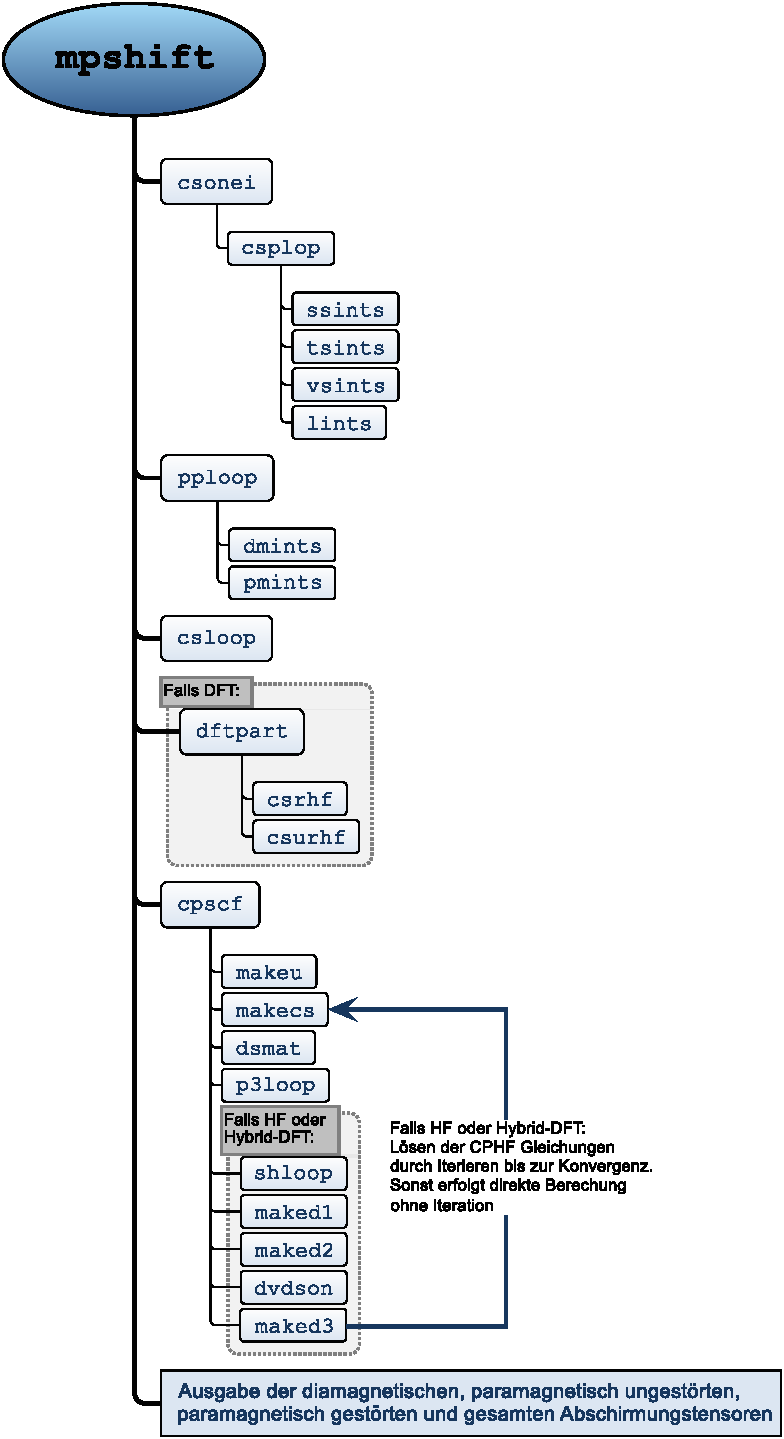
\includegraphics[width=0.75\textwidth]{programmstruktur_alt}
\captionsetup{figurewithin = chapter}
\captionsetup{font=small, labelfont=bf}\caption[Grundlegende Programmstruktur]{Schematische Darstellung der grundlegenden Programmstruktur des Moduls \texttt{mpshift} vor den Modifikationen, die im Laufe der vorliegenden Arbeit durchgeführt werden. In der Abbildung sind nur die wichtigsten Routinen enthalten.}
\label{abb:programmstrukur_alt}
\end{figure}


\chapter{Verbesserung der Effizienz}\label{effizienz}
CPU-Rechenzeit ist eine wertvolle Ressource und muss finanziert werden. Weiterhin erfreut es den (ungeduldigen) Anwender, wenn das Ergebnis einer quantenchemischen Rechnung möglichst schnell erhalten wird. Aus diesem Grund ist die Effizienzsteigerung immer ein aktuelles Forschungsgebiet. Eine Möglichkeit, Berechnungen effizienter durchzuführen, ist durch das Einführen von Näherungen gegeben. Diese Vereinfachen die zu berechnenden Größen und führen damit schneller zu Resultaten. Eine weit gebräuchliche Näherung ist mit der \ac{ri}-Näherung gegeben\supercite{vahtras1993integral}, welche im Ursprung auf Dunlap\supercite{dunlap1979some} und Whitten\supercite{whitten1973coulombic} zurückzuführen ist. Die Übertragung dieser Methode auf die Berechnung von chemischen Abschirmungskonstanten, sowie eine weitere Beschleunigung der Näherung durch eine Multipolentwicklung, sind in den folgenden Kapiteln \ref{ri} und \ref{marij} erläutert. Jedoch darf die Genauigkeit des Resultats nicht unter diesen Näherungsmethoden leiden. Aus diesem Grund wurde die Effizienz und die erhaltene Genauigkeit in Kapitel \ref{genauigkeit} untersucht. Optimierungen des Programmcodes, effizientes Abschätzen verschwindender Integralbeiträge und Parallelisierung des Programmcodes stellen weitere Möglichkeiten dar, um die Effizienz zu verbessern und sind in Kapitel \ref{paraopt} zusammengefasst. 

\bigskip
Unabhängig von der Verbesserung der Effizienz kann für die Implementierung von Integralen, welche nach den Komponenten des Magnetfeldes abgeleitet werden müssen, folgendes ausgenutzt werden. Als Beispiel sollen die abgeleiteten Kern-Elektron-Wechselwirkungsintegrale betrachtet werden. Mit der Beziehung $\vec{r}=\vec{r_\mu}+\vec{R}_\mu$ gilt für sie

\begin{equation}\label{eq:vmunudb}
\begin{aligned}
&\frac{\partial}{\partial B_\beta}\left(\left\langle\chi_{\mu}\left\vert\hat{V}_{\textrm{Ke}}\right\vert\chi_{\nu}\right\rangle\right)_{\vec{B}=0}=\frac{\iu}{2c}\left\langle\chi_{\mu}\left\vert\left(\vec{R}_{\mu\nu}\times\vec{r}\right)\hat{V}_{\textrm{Ke}}\right\vert\chi_{\nu}\right\rangle\\
&=\frac{\iu}{2c}\left\langle\chi_\mu^{\vec{B}=0}\left\vert\left(\vec{R}_{\mu\nu}\times\vec{r}_\mu\right)_\beta\hat{V}_{\textrm{Ke}}\right\vert\chi_\nu^{\vec{B}=0}\right\rangle+\frac{\iu}{2c}\left(\vec{R}_\mu\times\vec{R}_\nu\right)_\beta\left\langle\chi_{\mu}^{\vec{B}=0}\left\vert\hat{V}_{\textrm{Ke}}\right\vert\chi_{\nu}^{\vec{B}=0}\right\rangle.
\end{aligned}
\end{equation}

Bei der Verwendung von gewöhnlichen, atomzentrierten Basisfunktionen der Form

\begin{equation}
\chi_\mu^{\vec{B}=0}=x_\mu^l y_\mu^m z_\mu^n e^{-\zeta\vec{r}_\mu^2},
\end{equation}

wobei $\zeta$ der Exponent der Basisfunktion ist, können die Abgeleiteten Integrale aus den nicht abgeleiteten Integralen durch Multiplikation mit dem Faktor $\frac{\iu}{2c}\left(\vec{R}_\mu\times\vec{R}_\nu\right)$ (zweiter Term auf der rechten Seite in Gleichung (\ref{eq:vmunudb})) und aus den nicht abgeleiteten Integralen, bei denen entsprechend die l-Quantenzahl ($l$, $m$, $n$) um 1 erhöht wurde (zweiter Term auf der rechten Seite in Gleichung (\ref{eq:vmunudb})), berechnet werden. Letztere werden auch in ähnlicher Form (mit anderem Vorfaktor) bei der Berechnung des kartesischen Gradienten erhalten, sodass für ihre Berechnung vorhandene Gradientenroutinen modifiziert werden können. Alternativ lassen sie sich jedoch auch durch Modifikation der Routinen für die Berechnung der Energie erhalten. 

\section{Die RI-Methode für chemische Abschirmungskonstanten}\label{ri}
Die \ac{ri}-Näherung stellt in der \ac{scf}-Prozedur ein bewährtes Näherungsverfahren zur Berechnung der Zweielektronenintegrale dar. Diese setzen sich aus dem Coulombterm und dem Austauschterm zusammen und deren Berechnung ist der zeitaufwändigste Schritt während des Verfahrens. Insbesondere der Coulombterm lässt sich durch das Anwenden der \ac{ri}-Näherung deutlich effizienter berechnen. Dies gilt bereits für Basissätze von \textit{double}-$\zeta$ Qualität und wird für größere Basissätze noch effizienter. Prinzipiell kann die Näherung auch für den Austauschterm angewendet werden, die Rechenzeiten verkürzen sich jedoch erst deutlich bei größeren Basissätzen ab \textit{quadruple}-$\zeta$ Qualität. Wird nur der Coulombterm oder nur der Austauschbeitrag angenähert, so wird von \ac{ri}-J oder \ac{ri}-K gesprochen, bzw. \ac{ri}-JK wenn die Näherung für beide Terme angewendet wird. 

Auch bei der Berechnung chemischer Abschirmungskonstanten ist die Berechnung der abgeleiteten Zweielektronenintegrale zeitbestimmend. Dies gilt insbesondere dann, wenn reine \ac{dft}-Funktionale (d.h. keine Hybrid-Funktionale mit Hartree-Fock-Austausch) verwendet werden, da für sie im Rahmen der \textit{uncoupled}-\ac{dft} keine \ac{cphf}-Gleichungen gelöst werden müssen. Die \ac{ri}-Näherung lässt sich auch auf die abgeleiteten Zweielektronenintegrale übertragen, wobei die Näherung in dieser Arbeit lediglich auf den abgeleiteten Coulombterm übertragen wird. Das getrennte Berechnen der Coulomb- und Austauschterme hat weiterhin den Vorteil, dass für die konventionelle Berechnung des Austauschs eine effizientere Integralabschätzung angewendet werden kann. Dies ist durch den schnelleren Abfall des Austauschs im Vergleich zur Coulombwechselwirkung begründet. Folglich kann damit durch Anwenden der \ac{ri}-J-Näherung auch der Austausch effizienter berechnet werden. Weiteres dazu wird in Kapitel \ref{paraopt} erläutert. 
	\subsection{Theorie}
	An dieser Stelle sollen zunächst die grundlegende Idee der Näherung und die daraus resultierenden Formeln aus \supercite{vahtras1993integral} wiedergegeben werden. Im Anschluss daran folgt die Übertragung auf die nach den Komponenten des Magnetfeldes abgeleiteten Coulombintegrale. 
	
	Die Berechnung der Coulombintegrale skalieren formell mit der Anzahl der Baisfunktionen $N_\textrm{BF}$ wie $\mathcal{O}(N_\textrm{BF}^4)$. Durch Anwenden der \ac{ri}-Näherung lässt sich das formelle Skalierungsverhalten um eine Potenz erniedrigen. Die Vierzentrenintegrale lassen sich als Summe des Produkts von Zwei- und Dreizentrenintegralen schreiben, welche wie $\mathcal{O}(N_\textrm{BF}^2)$ und $\mathcal{O}(N_\textrm{BF}^3)$ skalieren. Um diese zu erreichen, wird das Produkt zweiter Basisfunktionen $\chi_\mu$ und $\chi_\nu$ durch die Linearkombination von sogenannten atomzentrierten Auxiliarbasisfunktionen $P$ angenähert
	
	\begin{equation}
	\gamma_{\mu\nu}=\chi_\mu\chi_\nu\approx\sum_PC^P_{\mu\nu}P=\tilde{\gamma}_{\mu\nu}.
	\end{equation}
	
	Durch die Minimierung des Fehlers
	\begin{equation}
	\delta\gamma_{\mu}\nu = \gamma_{\mu\nu}-\tilde{\gamma}_{\mu\nu}
	\end{equation}
	
	wird letztendlich ein genäherter Ausdruck für die Vierzentrenintegrale erhalten
	
	\begin{equation}\label{eq:munukalari}
	\left(\chi_\mu\chi_\nu\vert\chi_\kappa\chi_\lambda\right)\approx\sum_{PQ}^{N_{\textrm{AuxBF}}}\left(\chi_\mu\chi_\nu\vert P\right)\left(P\vert Q\right)^{-1}\left(Q\vert\chi_\kappa\chi_\lambda\right).		
	\end{equation}
	Für eine effiziente Berechnung der Matrixelemente der Coulombmatrix $J_{\mu\nu}$, wofür Gleichung (\ref{eq:munukalari}) noch mit der Dichtematrix $D_{\kappa\lambda}$ gespurt werden muss, wird zunächst die inverse $\left(P\vert Q\right)^{-1}$-Matrix gebildet und mit den Dreizentrenintegralen $\left(Q\vert\chi_\kappa\chi_\lambda\right)$ sowie der Dichtematrix zur intermediären Größe $\Gamma_P$ verarbeitet
	\begin{equation}
	\Gamma_P=\sum_Q^{N_{\textrm{AuxBF}}}\left(P\vert Q\right)^{-1}\sum_{\kappa\lambda}D_{\kappa\lambda}\left(Q\vert\chi_\kappa\chi_\lambda\right).
	\end{equation}
	Die eigentliche Berechnung von $J_{\mu\nu}$ erfolgt durch Spuren der Dreizentrenintegrale $\left(\chi_\mu\chi_\nu\vert P\right)$ mit $\Gamma_P$
	\begin{equation}
	J_{\mu\nu}=\sum_{\kappa\lambda}D_{\kappa\lambda}\left(\chi_\mu\chi_\nu\vert\chi_\kappa\chi_\lambda\right)\approx\sum_{P}^{N_{\textrm{AuxBF}}}\left(\chi_\mu\chi_\nu\vert P\right)\Gamma_P=J_{\mu\nu}^{\textrm{RI}}.
	\end{equation}
	Im Vergleich zu den Fehlern der Methoden sind die Fehler, die durch diese Näherung gemacht werden, klein und von wenig Bedeutung.\supercite{eichkorn1995auxiliary} Die \ac{ri}-Näherung lässt sich nun auch auf den nach den Komponenten des Magnetfeldes abgeleiteten Coulombterm übertragen. Wie bereits zuvor erwähnt, gilt
	
	\begin{equation}\label{eq:jmunudb}
	\begin{aligned}
	J_{\mu\nu}^{B_\beta}=&\frac{\partial}{\partial B_\beta}\left(\sum_{\kappa\lambda}D_{\kappa\lambda}\left(\chi_\mu\chi_\nu\vert\chi_\kappa\chi_\lambda\right)\right)_{\vec{B}=0}\\
	=&\sum_{\kappa\lambda}\left[D_{\kappa\lambda}^{B_\beta}\left(\chi_\mu^{\vec{B}=0}\chi_\nu^{\vec{B}=0}\vert\chi_\kappa^{\vec{B}=0}\chi_\lambda^{\vec{B}=0}\right)+D_{\kappa\lambda}\left(\overline{\chi_\mu\chi_\nu}\vert\chi_\kappa^{\vec{B}=0}\chi_\lambda^{\vec{B}=0}\right)_{\beta}\right.\\
    &+\left.D_{\kappa\lambda}\left(\chi_\mu^{\vec{B}=0}\chi_\nu^{\vec{B}=0}\vert\overline{\chi_\kappa\chi_\lambda}\right)_{\beta}\right]\\
    =&\sum_{\kappa\lambda}D_{\kappa\lambda}\left(\overline{\chi_\mu\chi_\nu}\vert\chi_\kappa^{\vec{B}=0}\chi_\lambda^{\vec{B}=0}\right)_{\beta}
	\end{aligned}
	\end{equation}
	da bei den Verschwindenden Termen in Gleichung (\ref{eq:jmunudb}) jeweils die Spur des Produkts einer symmetrischen mit einer antisymmetrischen Matrix sind. Es muss folglich nur die linke Seite des Integrals, also nur die Basisfunktionen $\chi_\mu$ und $\chi_\nu$, abgeleitet werden. Das Einsetzen der \ac{ri}-Näherung liefert daher
	
	\begin{equation}\label{eq:jmunudbri}
	\begin{aligned}
	J_{\mu\nu}^{B_\beta}\approx &\sum_{PQ}^{N_{\textrm{AuxBF}}}\left(\overline{\chi_\mu\chi_\nu}\vert P\right)_\beta\left(P\vert Q\right)^{-1}\sum_{\kappa\lambda}D_{\kappa\lambda}\left(Q\left\vert\chi_\kappa^{\vec{B}=0}\chi_\lambda^{\vec{B}=0}\right.\right)\\
	=&\sum_{P}^{N_{\textrm{AuxBF}}}\left(\overline{\chi_\mu\chi_\nu}\vert P\right)_\beta\Gamma_P=J_{\mu\nu}^{B\beta ,\textrm{RI}}.
	\end{aligned}
	\end{equation}
	\vfill
	\subsection{Implementierung}
	Die intermediäre Größe $\Gamma_P$, welche für die abgeleiteten Coulombintegrale in Gleichung (\ref{eq:jmunudbri}) benötigt wird, kann auf die ganz konventionelle Art berechnet werden, wie es beispielsweise auf für die Berechnung der Energie während des \ac{scf}-Verfahrens notwendig ist. Neben den Trivialitäten, wie dem Modifizieren des Moduls zum Einlesen der Auxiliarbasissatzinformationen, müssen zusätzlich noch die abgeleiteten Dreizentrenintegrale $\left(\overline{\chi_\mu\chi_\nu}\vert P\right)$ implementiert werden. Diese sind von der Form
	
	\begin{equation}\label{eq:3centintdb}
	\begin{aligned}
	\left(\left.\overline{\chi_\mu\chi_\nu}\right\vert P\right)_\beta=&\frac{\iu}{2c}\left(\left.\left(\vec{R}_{\mu\nu}\times\vec{r}\right)_\beta\chi_\mu^{\vec{B}=0}\chi_\nu^{\vec{B}=0}\right\vert P\right)\\
	=&\frac{\iu}{2c}\left(\left.\left(\vec{R}_{\mu\nu}\times\vec{r}_\mu\right)_\beta\chi_\mu^{\vec{B}=0}\chi_\nu^{\vec{B}=0}\right\vert P\right)\\
	&+\frac{\iu}{2c}\left(\left.\vec{R}_\mu\times\vec{R}_\nu\right)_\beta\left(\chi_\mu^{\vec{B}=0}\chi_\nu^{\vec{B}=0}\right\vert P\right)
	\end{aligned}
	\end{equation}
	und lassen sich damit aus den nicht abgeleiteten Integralen berechnen, wobei beachtet werden muss, dass die $l$-Quantenzahl für $\chi_\mu$ im ersten Term auf der rechten Seite in Gleichung (\ref{eq:3centintdb}) um 1 erhöht werden muss. Integrale dieser Form werden bereits in den Routinen zur Berechnung des kartesischen Gradienten mit \ac{ri}-Näherung benötigt. Diese Routinen wurden entsprechend modifiziert um alle nach den Komponenten des Magnetfeldes abgeleiteten Integrale zu erhalten. In der Abbildung \ref{abb:programmstrukur_ri} ist eine schematische Darstellung der wichtigsten übertragenen, modifizierten und neuen Routinen in das \texttt{mpshift} Modul gegeben. Alte Routinen sind in blau, neue Routinen in grün, modifizierte Routinen in orange und unverändert aus anderen Modulen übertragene Routinen in rot dargestellt. Die Funktion der einzelnen Routinen sei im Folgenden erläutert.
	
	\begin{itemize}[leftmargin=65pt]
	    \item[\texttt{riprep}:] Routine zur Vorbereitung der notwendigen Größen und Felder für die Berechnung von $J_{\mu\nu}^{B\beta ,\textrm{RI}}$ mit der \ac{ri}-Näherung. 
	    \item[\texttt{lp2sym}:] Berechnung der $\left(P\vert Q\right)$-Matrix.
	    \item[\texttt{sichol}:] Cholesky-Zerlegung der $\left(P\vert Q\right)$-Matrix, da für die spätere Verarbeitung nicht explizit die Inverse $\left(P\vert Q\right)^{-1}$-Matrix berechnet wird.
	    \item[\texttt{twoder}:] Treiberroutine zur Berechnung von $J_{\mu\nu}^{B_\beta ,\textrm{RI}}$. Es wird zunächst die intermediäre Größe $\Gamma_P$ aus der Cholesky-Zerlegung von $\left(P\vert Q\right)$ und aus $\Gamma_Q$ (siehe \texttt{lpdrc1}) berechnet und im Anschluss folgt die eigentliche Berechnung von $J_{\mu\nu}^{B_\beta ,\textrm{RI}}$.
	    \item[\texttt{lpdrc1}:] Berechnung der Dreizentrenintegrale. Diese werden direkt mit der Dichtematrix kontrahiert, sodass die Größe $\Gamma_Q=\sum_{\kappa\lambda}D_{\kappa\lambda}\left(Q\vert\chi_\kappa\chi_\lambda\right)$ erhalten wird.
	    \item[\texttt{cslp3\_omp}:] Übergeordnete Routine zur Unterscheidung zwischen sequentieller und paralleler Ausführung des Moduls.
	    \item[\texttt{cslp3}:] Berechnung der Abgeleiteten Dreizentrenintegrale $\left(\left.\overline{\chi_\mu\chi_\nu}\right\vert P\right)$. Schleife über alle Schalentripel $i,j,k$.
	    \item[\texttt{csasra3}:] Schleife über die primitiven Basisfunktionen $\chi_\mu^{\vec{B}=0}$ und $\chi_\nu^{\vec{B}=0}$ und primitiven Auxiliarbasisfunktionen $P$
	    \item[\texttt{csgasram}:] Berechnung der eigentlichen Dreizentrenintegrale für aktuelles Tripel primitiver Basisfunktionen $\chi_\mu^{\vec{B}=0}$ und $\chi_\nu^{\vec{B}=0}$ und primitiver Auxiliarbasisfunktion $P$ für das aktuelle Schalentripel $i,j,k$.
	    \item[\texttt{crosscs}:] Berechnung des Kreuzprodukts in Gleichung (\ref{eq:3centintdb}) für beliebige Schalenpaare $i,j$. Die Berechnung der Kreuzprodukte für die Schalenkombinationen $s,s$ und $s,p$ erfolgt explizit in \texttt{cspl3}.
	    \item[\texttt{dftfck}:] Addition der Beiträge der Schalenpaare $i,j$ auf die Fockmatrix.
	\end{itemize}
	
\begin{figure}[ht!]
\centering
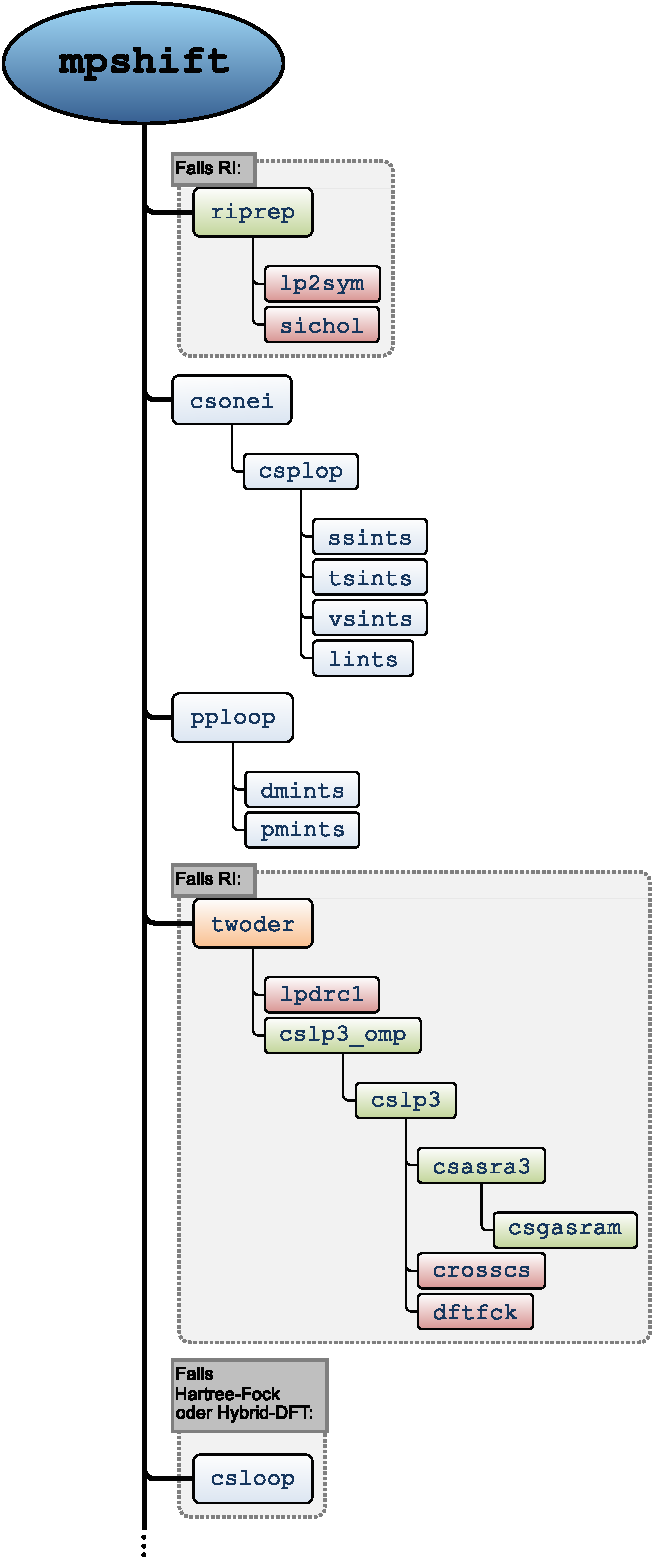
\includegraphics[width=0.6\textwidth]{programmstruktur_ri}
\captionsetup{figurewithin = chapter}
\captionsetup{font=small, labelfont=bf}\caption[\ac{ri}-J Routinen für chemische Abschirmungskonstanten]{Schematische Darstellung der wichtigsten Routinen für die \ac{ri}-Näherung zur Berechnung chemischer Abschirmungskonstanten im Modul \texttt{mpshift}. Alte Routinen sind in blau, neue Routinen in grün, modifizierte Routinen in orange und unverändert übertragene Routinen in rot dargestellt.}
\label{abb:programmstrukur_ri}
\end{figure}

\section{Die MARI-J Methode für chemische Abschirmungskonstanten}\label{marij}
Eine weitere Beschleunigung bei der Berechnung der Coulombintegrale lässt sich durch die \acf{marij} Näherung erhalten. Bei dieser Methode wird der Coulombbeitrag in einen Nahfeld und Fernfeld Beitrag aufgeteilt. Der Nahfeld Beitrag wird dabei durch die im vorherigen Kapitel beschriebene \ac{ri}-Näherung berechnet. Die Berechnung des Fernfeld Beitrages erfolgt mit Hilfe einer Multipolentwicklung und ist damit namensgebend für die Methode. Im Vergleich zu konventionellen \ac{ri}-Rechnungen konnte mit der \ac{marij} Methode eine bis zu 6,5-fache Beschleunigung, ohne einen nennenswerten Verlust an Genauigkeit, berichtet werden.\supercite{sierka2003fast}
	\subsection{Theorie}
	Dieser Abschnitt widmet sich der Berechnung des Fernfeld Beitrages für den Coulombterm und geht auf die Formulierungen von White und Head-Gordon\supercite{white1994derivation} zurück. Die folgende Darstellung folgt Referenz \supercite{sierka2003fast}, woraus die wesentlichen Formeln entnommen wurden. Zunächst kann der Abstand zweier Elektronen $\vert\vec{r}_1-\vec{r}_2\vert$ durch den Abstand zweiter Kerne $\vec{R}_{\mu\nu}=\vert\vec{R}_\mu-\vec{R}_\nu\vert$ und der entsprechenden Kern-Eelektron Abstände $\vec{r}_\mu$ und $\vec{r}_\nu$ ausdrücken
	\begin{equation}
	\frac{1}{\vert\vec{r}_1-\vec{r}_2\vert}=\frac{1}{\vert\vec{R}_{\mu\nu}-\vec{r}_\mu+\vec{r}_\nu\vert}=\sum_{l=0}^{\infty}\sum_{m=-l}^l O_{lm}(\vec{r}_\mu)\left[\sum_{j=0}^{\infty}\sum_{k=-j}^jB_{jk}^{lm}(\vec{R}_{\mu\nu})O_{jk}(\vec{r}_\nu)\right].
	\end{equation}
	Für einen gegebenen Punkt $\vec{r}=(r,\theta,\phi)$ in Kugelkoordinaten sind die Elemente $B_{jk}^{lm}(\vec{r})=M_{l+j,m+k}(\vec{r})$ und $O_{lm}(\vec{r})$ gegeben durch
	\begin{equation}
	O_{lm}(\vec{r})=\frac{r^l}{(l+\vert m\vert)!}P_{lm}(\cos \theta)e^{-\iu m\phi}
	\end{equation}
	und 
	\begin{equation}
	M_{l,m}(\vec{r})=\frac{(l-\vert m\vert)!}{r^{l+1}}P_{lm}(\cos \theta)e^{\iu m\phi}
	\end{equation}
	mit den entsprechenden Legendre-Polynomen $P_{lm}$. Auf diese Weise lässt sich die Coulombwechselwirkung zweier entfernter Ladungsverteilungen $\rho^O$ und $\rho^R$ entwickeln
	\begin{equation}\label{eq:marijexpansion}
	\begin{aligned}
	J_{OR}=&\frac{1}{2} \int\int\frac{\rho^O(\vec{r}_1)\rho^R(\vec{r}_2)}{\vert\vec{r}_1-\vec{r}_2\vert}=\frac{1}{2}\int\int\frac{\rho^O(\vec{r}_\mu)\rho^R(\vec{R}_{\mu\nu}+\vec{r}_\nu)}{\vert\vec{R}_{\mu\nu}-\vec{r}_\mu+\vec{r}_\nu\vert}\\
	=&\frac{1}{2}\sum_{l=0}^\infty\sum_{m=-l}^l\Omega_{lm}^O\left[\sum_{j=0}^\infty\sum_{k=-j}^jB_{jk}^{lm}(\vec{R}_{\mu\nu})\Omega_{jk}^P\right]=\frac{1}{2}\sum_{l=0}^\infty\sum_{m=-l}^l\Omega_{lm}^O\Xi_{lm}^P.
	\end{aligned}
	\end{equation}
	Die $\Xi_{lm}^P$ sind die Koeffizienten einer lokalen Taylor-Entwicklung des durch eine Ladungsverteilung am Punkt $P$ erzeugten Potentials um den Ursprung
	\begin{equation}
	\Xi_{lm}^P=\sum_{j=0}^\infty\sum_{k=-j}^jB_{jk}^{lm}(\vec{R}_{\mu\nu})\Omega_{jk}^P.
	\end{equation}
	Die in Gleichung (\ref{eq:marijexpansion}) auftretenden $\Omega_{lm}^O$ und $\Omega_{jk}^P$ sind die Multipolmomente mit ihrem jeweiligen Zentrum am Ort $\vec{O}$ bzw. $\vec{P}$. Im Rahmen der Basissatzentwicklung sind sie gegeben durch
	\begin{equation}\label{eq:multipole}
	\Omega^Q_{lm}=\sum_{\mu,\nu \in Q}D_{\mu\nu}\int\chi_\mu O_{lm}(\vec{r}-\vec{Q})\chi_{\nu}\diff \vec{r}.
	\end{equation}
	Der Ausdruck auf der rechten Seite von Gleichung (\ref{eq:marijexpansion}) hat den Vorteil, dass sich die Coulombwechselwirkung zweier Ladungsverteilungen nun durch die voneinander unabhängigen Multipolmomente berechnen lässt, da die Information über die gegenseitige Lage der Ladungsverteilungen nur noch in $B_{jk}^{lm}$ steckt. Sind die Multipolmomente einer Ladungsverteilung ein mal berechnet, so lässt sich mit ihnen die Coulombwechselwirkung mit allen anderen Ladungsverteilungen berechnen.\supercite{sierka2003fast} 
	\subsection{Implementierung}
Zur Gewährleistung der Eichinvarianz bei der Berechnung chemischer Abschirmungskonstanten mit der \ac{marij} Methode müssen anstelle gewöhnlicher Basisfunktionen ebenfalls \acp{giao} für Gleichung (\ref{eq:multipole}) verwendet werden. Die Ableitung von Gleichung (\ref{eq:multipole}) nach den Komponenten des Magnetfeldes beträgt dann

	\begin{equation}\label{eq:multipoledb}
	\begin{aligned}
	\left.\frac{\partial \Omega^Q_{lm}}{\partial B_\beta}\right\vert_{\vec{B}=0}=&\Omega^{Q,B_\beta}_{lm}=\frac{\iu}{2c}\sum_{\mu,\nu \in Q}D_{\mu\nu}\int\left(\vec{R}_{\mu\nu}\times\vec{r}\right)_\beta\chi_\mu^{\vec{B}=0} O_{lm}(\vec{r}-\vec{Q})\chi_{\nu}^{\vec{B}=0}\Diff3 \vec{r}\\
	=&\frac{\iu}{2c}\sum_{\mu,\nu \in Q}\left(\vec{R}_{\mu}\times\vec{R}_{\nu}\right)_\beta D_{\mu\nu}\int\chi_\mu^{\vec{B}=0}O_{lm}(\vec{r}-\vec{Q})\chi_{\nu}^{\vec{B}=0}\Diff3\vec{r}\\
	&+\frac{\iu}{2c}\sum_{\mu,\nu \in Q}D_{\mu\nu}\left(\vec{R}_{\mu\nu}\times\int\vec{r}_{\mu}\chi_\mu^{\vec{B}=0}O_{lm}(\vec{r}-\vec{Q})\chi_{\nu}^{\vec{B}=0}\Diff3\vec{r}\right)_\beta .
	\end{aligned}
	\end{equation}
	Dieser Ausdruck wird schließlich in Gleichung (\ref{eq:marijexpansion}) eingesetzt, wodurch der durch Multipolmomente genäherte Beitrag für den Coulombterm erhalten wird. Zur Berücksichtigung der \ac{marij} Beiträge wurde die Routine \texttt{twoder} um den Aufruf der Modifizierten Routine \texttt{fmmlpdrc2} erweitert. Deren Funktion sowie davon gerufener Unterroutinen sind im Folgenden erläutert. Eine schematische Darstellung der wichtigsten Routinen zur Berechnung der \ac{marij} Beiträge für chemische Abschirmungskonstanten ist in Abbildung \ref{abb:programmstrukur_marij} gezeigt.
	\begin{itemize}[leftmargin=70pt]
	\item[\texttt{initmulopt}:] Initialisierung für die Multipolnäherung. Sofern im \texttt{control}-File Optionen spezifiziert wurden, werden sie an dieser Stelle eingelesen und ersetzen die Standardwerte.
	\item[\texttt{auxmaxmom}:] Bestimmung der maximalen Drehimpulsquantenzahl in den Auxiliarbasisfunktionen.
	\item[\texttt{extdef}:] Bestimmung der Multipolmomentzentren für das Schalenpaar zweier Basisfunktionen.
	\item[\texttt{fmmlpdrc1}:] Berechnung des Fernfeld Beitrages zu $\Gamma_Q$ in der Multipolnäherung.
	\item[\texttt{fmmlpdrc2}:] Berechnung des Fernfeld Beitrages zur Coulombmatrix in der Multipolnäherung.
	\item[\texttt{auxmom2}:] Berechnung der Multipolmomente für die Auxiliarbasisfunktionen und anschließende Kontraktion mit den Elementen von $\Gamma_P$.
	\item[\texttt{mktayaux}:] Berechnung der Koeffizienten der lokalen Taylor-Entwicklung für die Auxiliarschalen.
	\item[\texttt{csmunumom}:] Für die Berechnung von chemischen Abschirmungskonstanten modifizierte Version von \texttt{munumom2}. Hier erfolgt die Berechnung des Fernfeld Beitrages zur Coulombmatrix in der Multipolnäherung durch Kontraktion der Taylor-Koeffizienten der Auxiliarbasisfunktionen mit den Multipolmomenten der Schalenpaare zweier Basisfunktionen.
	\item[\texttt{cssphmom}:] Für die Berechnung von chemischen Abschirmungskonstanten modifizierte Version von \texttt{sphmom}. Berechnung der Multipolintegrale.
	\item[\texttt{lsprim}:] Berechnung der Multipolintegrale für die primitiven Basisfunktionen $\int s O_{lm} s\Diff3\vec{r}$ bis $\int s O_{lm} l_{ij+2} \Diff3\vec{r}$ (vertikale Rekursion), wobei $l_{ij+2}$ die Summe der Drehimpulsquantenzahlen der $i$- und $j$-Schale $+2$ ist.
	\item[\texttt{cshorsph}:] Für die Berechnung von chemischen Abschirmungskonstanten modifizierte Version von \texttt{horsph}. Berechnung aller benötigten Integrale  $\int l_i O_{lm} l_j\Diff3\vec{r}$ durch horizontale Rekursion.
	\item[\texttt{cscross}:] Berechnung der Kreuzproduktterme aus den einzelnen Integralen um den vollständigen Beitrag aus der Multipolnäherung für die Coulombmatrix zu erhalten.
	\end{itemize}
	
\begin{figure}[ht!]
\centering
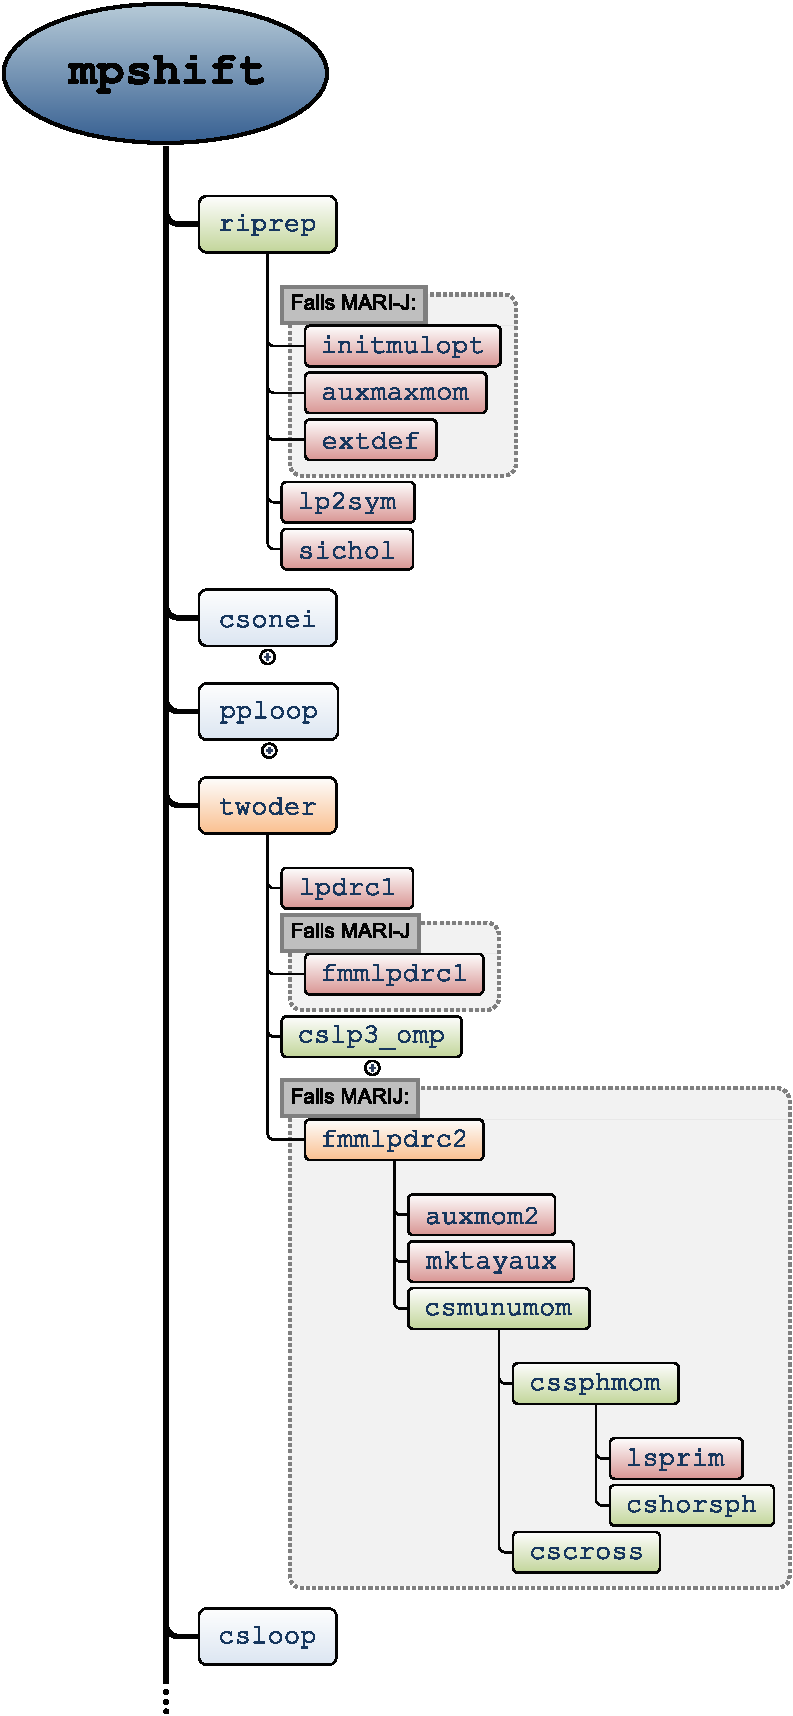
\includegraphics[width=0.7\textwidth]{programmstruktur_marij}
\captionsetup{figurewithin = chapter}
\captionsetup{font=small, labelfont=bf}\caption[\ac{marij} Routinen für chemische Abschirmungskonstanten]{Schematische Darstellung der wichtigsten Routinen für die \ac{marij}-Näherung zur Berechnung chemischer Abschirmungskonstanten im Modul \texttt{mpshift}. Alte Routinen sind in blau, neue Routinen in grün, modifizierte Routinen in orange und unverändert übertragene Routinen in rot dargestellt.}
\label{abb:programmstrukur_marij}
\end{figure}



\section{Parallelisierung und weitere Optimierungen}\label{paraopt}
Bei bestimmten Verbindungen kann es von Interesse sein, die chemischen Abschirmungskonstanten nur für eine Auswahl an Atomen zu berechnen. Beispielsweise wenn nur eine bestimmte Atomsorte von Interesse ist oder lediglich die chemische Verschiebung in einem bestimmten Bereich untersucht werden soll. In diesen Fällen kann es von Nutzen sein, nur die Beiträge für besagte Atome zu berechnen. Aus diesem Grund wurde das Modul \texttt{mpshift} um die Möglichkeit ergänzt, eine Vorauswahl der zu berechnenden Atome zu treffen. Im Programmcode selbst ist dies auf die einfache Weise realisiert, dass die Ableitungen nach den Komponenten der Kernmomente sowie der gesamte Abschirmungstensor nur für die ausgewählten Atome berechnet wird. Dies kann durch Hinzufügen des Keywords \texttt{\$nucsel} im \texttt{control}-File erreicht werden. Durch die Eingabe von \texttt{\$nucsel "N","Fe"} lassen sich beispielsweise die chemischen Abschirmungskonstanten für alle Sickstoff- und Eisenatome im Molekül berechnen. Mit \texttt{\$nucsel 1,3,5-8} erfolgt die Berechnung für die Atome Nummer 1,3,5-8 im \texttt{coord}-File. Sind in größeren organischen Molekülen, welche von Wasserstoff- und Kohlenstoffatomen dominiert sind, nur die $^1$H bzw. $^13$C Abschirmungskonstanten von Interesse, so bringt dieses vorgehen in der Regel jedoch kaum eine Zeitersparnis und es können direkt alle Atome berechnet werden. Umgekehrt lassen sich auf diese Weise auch Elemente aus der Rechnung herausnehmen, welche ohnehin nicht von Interesse sind, aber gegebenenfalls für ein schlechtes Konvergenzverhalten während der \ac{cphf}-Iterationen sorgen.

\bigskip
Das bisherige, standardmäßige Auswählen des ersten Atoms im \texttt{coord}-File für den Konvergenztest bei den \ac{cphf}-Iterationen lässt sich ebenfalls optimieren. In der Praxis hat sich herausgestellt, dass insbesondere für schwere Elemente mehr Iterationen benötigt werden, bis die Konvergenz erreicht wurde. Dies liegt auch daran, dass die Absolutwerte für die chemischen Abschirmungskonstanten dieser Elemente mit zunehmender Ordnungszahl steigen. Die Konvergenz wurde aber Standardmäßig auf eine Änderung von weniger als \unit[$1\times 10^{-2}$]{ppm} gesetzt, unabhängig von Element. Hierfür wurde ein Faktor eingeführt, welcher die Ordnungszahl des entsprechenden Elements berücksichtigt und die Konvergenz für Elemente mit hoher Ordnungszahl ein wenig lockert. Weiterhin hat sich herausgestellt, dass Atome die weit vom Koordinatenursprung entfernt sind, ebenfalls länger bis zur Konvergenz benötigen. Daher erfolgt die Atomauswahl für den Konvergenztest bei den \ac{cphf}-Iterationen dermaßen, dass zunächst das schwerste Element im Molekül gesucht wird. Sollte es davon mehrere geben, dann wird das Atom ausgewählt, welches am weitesten vom Ursprung entfernt liegt. Dieses Vorgehen hat den Vorteil, dass in der Regel nur in den letzten beiden Iterationen die chemische Verschiebung für alle Atome berechnet werden muss, um zu überprüfen, ob alle Atome bereits konvergiert sind. Da der kritischste Fall zu diesem Zeitpunkt in der Regel bereits zur Konvergenz gebracht werden konnte, ist dies in der Regel gegeben.

\bigskip
Wird die \ac{ri} bzw. \ac{marij}-Methode in einer Hartree-Fock bzw. Hybrid-\ac{dft} Rechnung verwendet, so wird der Austauschbeitrag unabhängig vom Coulombbeitrag berechnet. Für ersteren kann jedoch eine effizientere Integralabschätzung\supercite{ochsenfeld1998linear} angewendet werden, als für den Coulombbeitrag. Aus diesem Grund wurden die Integralabschätzungen aus der Routine \texttt{shloop\_k}, welche ungestörten Austauschmatrixelemente in einer \ac{scf} oder während der \ac{cphf}-Iterationen berechnet, in die Routine \texttt{csloop} übertragen. Auf diese Weise kann die Berechnung kleiner bzw. später verschwindender Matrixelemente vermieden werden. Des Weiteren wurde die Routine \texttt{shloop}, welche in der Routine \texttt{cpscf} zur Berechnung der ungestörten Zweielektronenintegrale gerufen wird, durch die Routine \texttt{hf\_k} ersetzt. Das ist darin begründet, dass die Spur des Produkts der symmetrischen Coulombmatrix und der antisymmetrischen Dichtematrix verschwindet, und daher wird der Coulombbeitrag an dieser Stelle nicht mehr benötigt. Lediglich der Austauschbeitrag muss berechnet werden, wofür die Routine \texttt{hf\_k} optimiert ist. Beim iterativen Lösen der \ac{cphf}-Gleichungen kann zusätzlich durch Bilden von Differenzdichten (aus der aktuellen und vorherigen Iteration) profitiert werden. 

\bigskip
Neben einer effizienten Programmierung und dem Einführen von Näherungen wie beispielsweise bei der \ac{ri} bzw. \ac{marij}-Methode, kann die Wartezeit des Nutzers auch durch eine Parallelisierung des Programmcodes reduziert werden. Dies ist insofern von besonderer Bedeutung, dass heutige Computer immer mehr CPUs zur Verfügung haben. Selbst in gewöhnlichen Desktop PCs oder Notebooks finden sich häufig mindestens 4 CPUs. Aus diesem Grund wurden die zeitaufwändigsten Routinen im \texttt{mpshift} Modul mit OpenMP\supercite{dagum1998openmp} in Zusammenarbeit mit Fabian Mack parallelisiert. Im Einzelnen betrifft dies die Routinen \texttt{becke}, \texttt{csloop}, \texttt{cslp3\_omp}, \texttt{csplop},\texttt{shloop\_k} \texttt{p3loop} und \texttt{pploop}. Die Routinen \texttt{csplop}, \texttt{p3loop} und \texttt{pploop} besitzen üblicherweise folgende grundlegende Schleifenstruktur.\\
\\
\texttt{do i=1,N$_{\texttt{Schal}}$}\\ 
\null\quad\texttt{do j=1,N$_{\texttt{Schal}}$}\\ 
\null\quad\quad\texttt{do $\mu$=1,N$_{\texttt{Prim BF}}$}\\ 
\null\quad\quad\quad\texttt{do $\mu$=1,N$_{\texttt{Prim BF}}$}\\
\null\quad\quad\quad\quad \texttt{Auszuführender Programmcode}\\ 
\null\quad\quad\quad\texttt{end do}\\ 
\null\quad\quad\texttt{end do}\\ 
\null\quad\texttt{end do}\\ 
\texttt{end do}\\
\\
Die äußeren beiden Schleifen laufen dabei über alle Schalen N$_{\texttt{Schal}}$ und die beiden inneren Schleifen laufen über die primitiven Basisfunktionen. Für die Routine \texttt{cslp3\_omp} kommt jeweils eine weitere Schleife für die Auxiliarschale und die primitiven Auxiliarbasisfunktionen hinzu. Bei den Vierzentrenroutinen \texttt{csplop} und \texttt{shloop\_k} sind es jeweils zwei weitere Schleifen für die Schalen und die primitiven Basisfunktionen. Bei der Parallelisierung wurde nun in der Regel so vorgegangen, dass die äußersten Schleifen über die Schalen parallelisiert wurden:\\
\\
\texttt{\$OMP PARALLEL}\\
\texttt{\$OMP DO SCHEDULE (DYNAMIC)}\\
\texttt{do i=1,N$_{\texttt{Schal}}$}\\ 
\null\quad\texttt{do j=1,N$_{\texttt{Schal}}$}\\ 
\null\quad\quad\texttt{do $\mu$=1,N$_{\texttt{Prim BF}}$}\\ 
\null\quad\quad\quad\texttt{do $\mu$=1,N$_{\texttt{Prim BF}}$}\\
\null\quad\quad\quad\quad \texttt{Auszuführender Programmcode}\\ 
\null\quad\quad\quad\texttt{end do}\\ 
\null\quad\quad\texttt{end do}\\ 
\null\quad\texttt{end do}\\ 
\texttt{end do}\\
\texttt{\$OMP END DO}\\
\texttt{\$OMP END PARALLEL}\\
\\


\chapter{Erweiterung der Funktionalität}\label{funktionalität}
Das Modul \texttt{mpshift} umfasste bisher die Möglichkeit zur Berechnung von chemischen Abschirmungskonstanten in Molekülen ohne schwere Elemente (ab etwa $Z$=36) in der Gasphase. Diese Berechnungen konnten auf Hartree-Fock, \ac{dft} (für \ac{lda}- und \ac{gga}-Funktionale) und \ac{mp2} Nievau durchgeführt werden. Des Weiteren konnte die nach den Komponenten des Magnetfeldes abgeleitete Dichtematrix dem externen Programm \ac{gimic} zur Weiterverarbeitung bereit gestellt werden. Die folgenden Kapitel beschreiben die Erweiterung der Funktionalität des Moduls die im Rahmen dieser Arbeit implementiert wurden. Im Einzelnen sind dies die Berücksichtigung relativistischer Effekte auf Nachbaratome in Molekülen mit schweren Elementen durch relativistische \acp{ecp}, die Einbeziehung von Umgebungseffekten sowie die Bereitstellung der magnetischen Response zur Berechnung von \ac{vcd}-Spektren. Weiterhin wurde das Modul um die Möglichkeit ergänzt, \ac{mgga}-Funktionale für die Berechnung der Abschirmungskonstanten auf \ac{dft}-Niveau zu verwenden. Die eigentliche Implementierung dieses letzten Punktes erfolgte jedoch nicht von mir, sondern von Fabian Mack im Rahmen seiner Masterarbeit.\supercite{mack2017} 


\section{Berücksichtigung von Umgebungseffekten}
Isotrope chemische Verschiebungen werden üblicherweise in Lösung gemessen. Je nachdem wie stark das zu untersuchende Molekül mit dem Lösungsmittel wechselwirkt, hat das Lösungsmittel einen mehr oder weniger stark ausgeprägten Einfluss auf das gemessene Spektrum. Das \ac{cosmo}\supercite{klamt1993cosmo}, ein Kontinuumsmodell, ist in der Quantenchemie ein bewährtes Verfahren zur Berücksichtigung von Umgebungseffekten. Neben den Einflüssen des Lösungsmittels lassen sich damit auch für Ionen die Ladungen kompensieren, ohne die Gegenionen explizit mitrechnen zu müssen. Insbesondere hoch geladene Anionen lassen sich ohne eine solche Ladungskompensation nur schwer oder gar nicht berechnen. 

Neben \ac{cosmo} besteht auch die die Möglichkeit, Lösungsmittelmoleküle explizit in die Berechnung mit einzubeziehen. Soll eine größere Anzahl an Lösungsmitteln explizit betrachtet werden, um beispielsweise eine vollständige Solvatationshülle um das gelöste Molekül zu erhalten, so bieten sich \ac{md}-Simulationen an. Aus diesen Simulationen für ein bestimmtes Zeitintervall, lassen sich einzelne Schnappschüsse der Molekülkoordinaten extrahieren. Für diese einzelnen Koordinaten lassen sich dann \textit{ab initio} Rechnungen durchführen. Ein Vergleich solch unterschiedlicher Ansätze ist in Kapitel \ref{lömitest} für das Acetonmolekül in Wasser zu finden. 
	\subsection{Theorie}
	In einem Kontinuum-Lösungsmittel-Model (englisch \ac{csm}), wie dem \ac{cosmo}, wird das zu betrachtende Lösungsmittel durch seine Dielektrizitätskonstante $\varepsilon$ beschrieben. Das gelöste Molekül stellt dabei einen Hohlraum im dielektrischen Kontinuum dar und polarisiert das dielektrische Medium aufgrund seiner Ladungsverteilung. Zur Beschreibung der Reaktion des dielektrischen Mediums auf diese Polarisierung, werden auf der Oberfläche des durch das gelöste Molekül entstandenen Hohlraums sogenannte \textit{screening}-Ladungen generiert. In der Praxis wird also in einem bestimmten Abstand eine Hülle um das gelöste Molekül gelegt und auf der Oberfläche dieser Hülle befinden sich diese Ladungen. Beim \ac{cosmo} wird nun die Nebenbedingung eingeführt, dass das elektrostatische Potential auf der Oberfläche dieser Hülle verschwinden soll, was einem idealen Lösungsmittel mit unendlicher Dielektrizitätskonstante $\varepsilon=\infty$ entspricht. Das gesamte elektrostatische Potential $\vec{\phi}^{\textrm{Tot}}$ setzt sich aus dem Beitrag des gelösten Moleküls $\vec{\phi}^{\textrm{Mol}}$ und dem Beitrag der \textit{screening}-Ladungen $\boldsymbol{A}\vec{q}$. $\vec{\phi}^{\textrm{Mol}}$ beinhaltet dabei sowohl die Beiträge der Elektronen, als auch die der Kerne. Der Vektor $\vec{q}$ enthält die insgesamt $N_{\textrm{SL}}$ \textit{screening}-Ladungen und die Matrix $\boldsymbol{A}$ beinhaltet die Coulombwechselwirkung der \textit{screening}-Ladungen untereinander. Mit der Bedingung des verschwindenden elektrostatischen Potentials folgt daher
	
	\begin{equation}
	\vec{\phi}^{\textrm{Tot}}=\vec{\phi}^{\textrm{Mol}}+\boldsymbol{A}\vec{q}=0,
	\end{equation}
	
wodurch sich die \textit{screening}-Ladungen definieren lassen
	\begin{equation}
	\vec{q}=\boldsymbol{A}^{-1}\vec{\phi}^{\textrm{Mol}}
	\end{equation}
Um nun Lösungsmittel mit unterschiedlichen Dielektrizitätskonstanten betrachten zu können, wird ein Skalierungsfaktor $f(\varepsilon)$ eingeführt
	\begin{equation}
	f(\varepsilon)=\frac{\varepsilon-1}{\varepsilon+\frac{1}{2}}
	\end{equation}
und damit lassen sich die entsprechenden \textit{screening}-Ladungen $\vec{q}(\varepsilon)$ erhalten
	\begin{equation}
	\vec{q}(\varepsilon)=\vec{q}(\varepsilon=\infty)f(\varepsilon).
	\end{equation}
Die Abweichungen aufgrund der hier gewählten Nebenbedingung des verschwindenden elektrostatischen Potentials im Vergleich zu den eigentlich viel komplexeren Nebenbedingungen ist sehr gering.\supercite{klamt1993cosmo} Dies gilt insbesondere für Lösungsmittel mit großen Dielektrizitätskonstanten, wie beispielsweise Wasser.

Bei der Berechnung chemischer Abschirmungskonstanten müssen die erzeugten Punktladungen auf der Oberfläche der Hülle um das gelöste Molekül ebenfalls berücksichtigt werden. Die \textit{screening}-Ladungen ergeben einen zusätzlichen Energiebeitrag $E^{\textrm{SM}}$ für den Einelektronenteil\supercite{cammi1999nuclear}

	\begin{equation}\label{eq:esm}
	E^{\textrm{SM}}=\sum_{l}^{N_{\textrm{SL}}}\int\frac{q_l\rho(\vec{r})}{\vert\vec{t}_l-\vec{r}\vert}\diff\vec{r}=\sum_{\mu\nu}D_{\mu\nu}\underbrace{\sum_l^{N_{\textrm{SL}}}\int\frac{q_l\chi_\mu\chi_\nu}{\vert\vec{t}_l-\vec{r}\vert}\diff\vec{r}}_{V_{\mu\nu}^{\textrm{SM}}}.
	\end{equation}
mit den Positionen $\vec{t}_l$ der \textit{screening}-Ladungen. Für die chemischen Abschirmungskonstanten wird daher die Ableitung von Gleichung (\ref{eq:esm}) nach den Komponenten des Magnetfeldes benötigt. Dies führt schließlich zu

	\begin{equation}\label{eq:esmdb}
	E^{\textrm{SM},B_\beta}=\sum_{\mu\nu}D_{\mu\nu}\underbrace{\frac{\iu}{2c}\sum_l^{N_{\textrm{SL}}}\int\left(\vec{R}_{\mu\nu}\times\vec{r}\right)\frac{q_l\chi_\mu^{\vec{B}=0}\chi_\nu^{\vec{B}=0}}{\vert\vec{t}_l-\vec{r}\vert}\diff\vec{r}}_{V_{\mu\nu}^{\textrm{SM},B_\beta}}.
	\end{equation}
	
	\subsection{Implementierung}
	Bei genauer Betrachtung von Gleichung (\ref{eq:esmdb}) fällt auf, dass die $V_{\mu\nu}^{\textrm{SM},B_\beta}$ die selbe Form haben wie die nach den Komponenten des Magnetfeldes abgeleitete Kern-Elektron-Wechselwirkung $V_{\textrm{Ke}\mu\nu}^{B_\beta}$. Zur Implementierung der \ac{cosmo} Beiträge bei der Berechnung chemischer Abschirmungskonstanten können daher die bereits bestehenden Routinen zur Berechnung des letztgenannten Beitrages modifiziert werden. Es ist dabei lediglich darauf zu achten, dass anstelle der Kernladungen die \textit{screening}-Ladungen und anstelle der Kernpositionen die Positionen der \textit{screening}-Ladungen an die entsprechende Routine übergeben werden. In der bei der Verwendung von \ac{cosmo} zur Berechnung von chemischen Abschirmungskonstanten wird daher die Routine \texttt{vsints} ein weiteres Mal von der Routine \texttt{csplop} mit den entsprechenden Feldern gerufen. 
	
Grundsätzlich lassen sich auf diese Weise die Beiträge von beliebige Punktladungen berechnen. Anstelle von \ac{cosmo}, was Punktladungen auf einer Hülle um das gelöste Molekül generiert, besteht daher auch die Möglichkeit die elektrostatische Wechselwirkung expliziter Lösungsmittelmoleküle durch Punktladungen zu ersetzen. Dafür können einzelne Momentaufnahmen aus \ac{md}-Simulationen verwendet werden. An die Positionen der Atome der Lösungsmittel werden Punktladungen gesetzt. Der Betrag der jeweiligen Ladung kann beispielsweise durch eine Populationsanalyse wie Mulliken\supercite{mulliken1955electronic} oder \ac{npa}\supercite{reed1985natural} bzw. durch einen \ac{esp}-Fit\supercite{singh1984approach} für das isolierte Lösungsmittelmolekül bestimmt werden. Die entsprechenden Koordinaten und Ladungen werden schließlich wieder an die Routine \texttt{vsints} übergeben. Eine Alternative zu den Punktladungen sind gaußförmig verschmierte Ladungen. Die dafür notwendigen Dreizentrenintegrale wurden bereits für die \ac{ri}-Näherung benötigt und können wiederverwendet werden. Um dies zu gewährleisten wird die Routine \texttt{csonei} um einen Aufruf der Routine \texttt{cslp3} erweitert. Im Vergleich zu punktförmigen Ladungen lässt sich dadurch eine etwas weichere Ladungsverteilung generieren. 

Die unterschiedlichen Möglichkeiten zur Einbeziehung von Lösungsmitteleffekten wurden am Beispiel des Acetonmoleküls in Wasser untersucht und ist im folgenden Kapitel erläutert.
	\subsection{Testrechnungen}\label{lömitest}
	
\section{Skalar-relativistische Effekte durch effektive Kernpotentiale}
Für schwere Atome nimmt mit steigender Kernladungszahl der Einfluss relativistischer Effekte zu. Diese relativistischen Einflüsse haben ihren Ursprung in Kernnähe schwerer Atome. Sie übertragen sich jedoch auch auf die Valenzschalen der entsprechenden Atome und haben damit auch einen Einfluss auf die chemische Verschiebung an benachbarten Atomen. Die vollrelativistische Berechnung im Rahmen vier- oder zweikomponentiger Methoden (wie beispielsweise das X2C-Verfahren) ist sehr aufwändig. Eine alternative Berücksichtigung skalarrelativistischer Effekte ist durch die Verwendung von sogenannten \acp{ecp}\supercite{cundari1996effective,frenking2007pseudopotential} gegeben. Hierbei werden die Elektronen in den Rumpforbitalen durch ein entsprechend gefittetes Potential beschrieben und nur die Valenzelektronen explizit betrachtet. Aufgrund der fehlenden kernnahen Elektronen haben chemische Abschirmungskonstanten, welche für Atome mit einem \ac{ecp} berechnet wurden, keine physikalische Bedeutung. Die Rumpfelektronen liefern den größten Beitrag zur Abschirmung und daher wird diese stark unterschätzt. Wird der durch das \ac{ecp} beschriebene Bereich nicht zu groß gewählt, d.h. sogenannte \textit{small core} \acp{ecp} verwendet, dann kann jedoch bei der Berechnung relativer chemischer Verschiebungen davon ausgegangen werden, dass sich der fehlende kernnahe Beitrag aufhebt.\supercite{van2012use} In diesem Zusammenhang untersuchten Moore und Healy\supercite{moore1995ab} die Abhängigkeit der Titan Abschirmung in Titan-Tetrahalogeniden von allelektornen Basissätzen sowie \acp{ecp} und kamen zu dem Schluss, dass die absoluten Abschirmungen stark von der gewählten Basis abhängen, die relativen chemischen Verschiebungen jedoch weitgehend unabhängig davon sind. Bagno und Bonchio konnten ebenfalls zeigen, dass sich die chemischen Verschiebungen, berechnet mit \acp{ecp}, von Wolfram\supercite{bagno2000effective} und Ruthenium\supercite{bagno2002dft} gut mit experimentell gemessenen Daten korrelieren lassen. Problematisch ist jedoch, dass die so erhaltenen chemischen Verschiebungen zunächst an experimentell gemessene Verschiebungen gefittet werden müssen, um eine Korrelation herzustellen. Erst damit lassen sich Aussagen über die chemische Verschiebung in unbekannten Verbindungen treffen. Für die Berechnung von chemischen Abschirmungskonstanten an benachbarten Atomen schwerer Atome können die \acp{ecp} jedoch problemlos verwendet werden.
	\subsection{Theorie}
	Eine eichinvariante Implementierung für \acp{ecp} wurde von van Wüllen\supercite{van2012use} vorgestellt und wichtigsten darin abgeleiteten Gleichungen sollen an dieser Stelle wiedergegeben werden. 
	
	Der Einelektronenhamiltonoperator im Magnetfeld $\vec{B}$ setzt sich aus dem ungestörten Hamiltonoperator $\hat{h}^0$ in Abwesenheit des Magnetfeldes sowie weiteren Termen linear, quadratisch usw. in $\vec{B}$ zusammen. Für die chemische Verschiebung werden jedoch nur Terme linear in $\vec{B}$ benötigt, daher ist $\hat{h}$ hier
	\begin{equation}\label{eq:heinel}
	\begin{aligned}
	\hat{h}=&\hat{h}^0+\hat{h}^{10}\\
	\hat{h}^0=&\frac{1}{2}\vec{p}^{\,2}+\hat{V}_{\textrm{Ke}}\\
	\hat{h}^{10}=&\frac{1}{2c}\left(\left(\vec{r}-\vec{R}_E\right)\times\vec{p}\right)\cdot\vec{B}.
	\end{aligned}
	\end{equation}
	Wie bereits zuvor in Kapitel \ref{theo:nmr} erwähnt, kannn der Eichursprung willkürlich gewählt werden und der Hamiltonoperator ist genau dann eichinvariant, wenn für unterschiedliche Eichursprünge die selben Werte magnetischer Eigenschaften berechnet werden. Dies ist dann erfüllt, wenn der Hamiltonoperator $\hat{\tilde{h}}$ mit dem Eichursprung $\vec{R}_{\tilde{E}}$ aus $\hat{h}$ durch eine unitäre Transformation der Form
	\begin{equation}\label{eq:trans}
	\hat{\tilde{h}}=\exp\left(\iu\Lambda_{\tilde{E}}\right)\hat{h}\exp\left(-\iu\Lambda_{\tilde{E}}\right),
	\end{equation}
	mit 
	\begin{equation}
	\begin{aligned}
	\Lambda_{\tilde{E}}=&\frac{1}{2c}\left(\left(\vec{R}_{\tilde{E}}-\vec{R}_E\right)\times\vec{r}\right)\cdot\vec{B}\\
	=&\frac{1}{2c}\left(\vec{B}\times\left(\vec{R}_{\tilde{E}}-\vec{R}_E\right)\right)\cdot\vec{r}
	\end{aligned}
	\end{equation}
	erhalten werden kann. Zur Bestimmung von $\hat{\tilde{h}}$ wird dessen Wirkung auf eine Funktion $f(\vec{r})$ betrachtet. Aus der unitären Transformation folgt
	
	\begin{equation}\label{eq:transh}
	\begin{aligned}
	\hat{\tilde{h}}f(\vec{r})=&\exp\left(\iu\Lambda_{\tilde{E}}\right)\hat{h}\exp\left(-\iu\Lambda_{\tilde{E}}\right)f(\vec{r})\\
	=&\exp\left(\iu\Lambda_{\tilde{E}}\right)\hat{h}^0\exp\left(-\iu\Lambda_{\tilde{E}}\right)f(\vec{r})+\exp\left(\iu\Lambda_{\tilde{E}}\right)\hat{h}^{10}\exp\left(-\iu\Lambda_{\tilde{E}}\right)f(\vec{r})
	\end{aligned}
	\end{equation}
	Für den ersten Term auf der rechten Seite von Gleichung (\ref{eq:transh}) ergibt sich
	\begin{equation}\label{eq:transh1}
	\begin{aligned}
	&\exp\left(\iu\Lambda_{\tilde{E}}\right)\hat{h}^0\exp\left(-\iu\Lambda_{\tilde{E}}\right)f(\vec{r})\\
	=&\exp\left(\iu\Lambda_{\tilde{E}}\right)\frac{-\iu}{2}\vec{p}\left[\frac{-\iu}{2c}\left(\vec{B}\times\left(\vec{R}_{\tilde{E}}-\vec{R}_E\right)\right)\exp\left(-\iu\Lambda_{\tilde{E}}\right)f(\vec{r})\right]\\
	&+\exp\left(\iu\Lambda_{\tilde{E}}\right)\frac{1}{2}\vec{p}\left[\exp\left(-\iu\Lambda_{\tilde{E}}\right)\vec{p}\left(f(\vec{r})\right)\right]+\hat{V}_{\textrm{Ke}}f(\vec{r})\\
	=&-\frac{1}{4c}\left(\vec{B}\times\left(\vec{R}_{\tilde{E}}-\vec{R}_E\right)\right)\vec{p}\left(f(\vec{r})\right)
	-\frac{1}{4c}\left(\vec{B}\times\left(\vec{R}_{\tilde{E}}-\vec{R}_E\right)\right)\vec{p}\left(f(\vec{r})\right)\\
	&+\frac{1}{2}\vec{p}^{\,2}f(\vec{r})+\hat{V}_{\textrm{Ke}}f(\vec{r})\\
	=&\frac{-1}{2c}\left(\vec{B}\times\left(\vec{R}_{\tilde{E}}-\vec{R}_E\right)\right)\vec{p}\left(f(\vec{r})\right)+\hat{h}^0f(\vec{r}),
	\end{aligned}
	\end{equation}
	und für den zweiten Term
	\begin{equation}\label{eq:transh2}
	\begin{aligned}
	\exp\left(\iu\Lambda_{\tilde{E}}\right)\hat{h}^{10}\exp\left(-\iu\Lambda_{\tilde{E}}\right)f(\vec{r})=&\frac{1}{2c}\left(\vec{B}\times\left(\vec{r}-\vec{R}_E\right)\right)\cdot\vec{p}\left(f(\vec{r})\right)\\
	&+\frac{1}{2c}\left(\vec{B}\times\left(\vec{r}-\vec{R}_E\right)\right)\cdot\frac{-1}{2c}\left(\vec{B}\times\left(\vec{R}_{\tilde{E}}-\vec{R}_E\right)\right)f(\vec{r})\\
	=&\hat{h}^{10}f(\vec{r})+\mathcal{O}(\vec{B}^{\,2}).
	\end{aligned}
	\end{equation}
	Für den Hamiltonoperator $\hat{\tilde{h}}$ folgt aus den Gleichungen (\ref{eq:transh1}) und (\ref{eq:transh2})
	\begin{equation}
	\begin{aligned}
	\hat{\tilde{h}}=&\hat{h}^0+\hat{h}^{10}-\frac{1}{2c}\left(\vec{B}\times\left(\vec{R}_{\tilde{E}}-\vec{R}_E\right)\right)\vec{p}\\
	=&\hat{h}^0+\frac{1}{2c}\left(\left(\vec{r}-\vec{R}_{\tilde{E}}\right)\times\vec{p}\right)\cdot\vec{B}
	\end{aligned}
	\end{equation}
	
	wobei die in $\vec{B}$ quadratischen Terme hier erneut weggelassen wurden. Der Eichursprung wurde durch die Transformation also von $\vec{R}_E$ auf $\vec{R}_{\tilde{E}}$ verschoben. Für diese Herleitung wurde davon ausgegangen, dass die Kern-Elektron-Wechselwirkung ein lokales Potential ist und daher nicht mit $\vec{r}$ kommutiert. Dies ist nur gültig, solange keine \acp{ecp} verwendet werden. Im letzteren Fall ist der Einelektronenhamiltonoperator aus Gleichung (\ref{eq:heinel}) durch
	
	\begin{equation}
	\hat{h}^0=\frac{1}{2}\vec{p}^{\,2}-\sum_K \left(\frac{Z_K^{\textrm{eff}}}{\vec{r}_K}+\hat{V}^{\textrm{ECP},K}\right)
	\end{equation}
	gegeben. Die Valenzelektronen, die nicht durch das \ac{ecp} beschrieben werden, erfahren dann nur noch eine verminderte effektive Kernladung $Z_K^{\textrm{eff}}$. Für die \acp{ecp} ist das Potential durch eine Summe atomarer Beiträge geben und diese haben die Form\supercite{mcmurchie1981calculation,cao2010relativistic}
	\begin{equation}\label{eq:ecpotential}
	\hat{V}^{\textrm{ECP},K}=\sum_{l=0}^{\infty}\hat{V}^{\textrm{ECP},K}_l\hat{P}_l^K,
	\end{equation}
	mit dem Projektionsoperator
	\begin{equation}
	\hat{P}_l^K=\sum_{m=-l}^l\vert lm\rangle\langle lm\vert
	\end{equation}
	und den Kugelflächenfunktionen $\vert lm\rangle$. Für $l\geq L$ unterscheiden sich die $\hat{V}^{\textrm{ECP},K}_l$ kaum mehr, wobei $L-1$ die größte, in den Kernorbitalen auftretende Drehimpulsquantenzahl ist. Mit der Annahme $\hat{V}^{\textrm{ECP},K}_l=\hat{V}^{\textrm{ECP},K}_L$ für $l\geq L$ folgt schließlich\supercite{kahn1972ab}
	\begin{equation}
	\hat{V}^{\textrm{ECP},K}=\hat{V}^{\textrm{ECP},K}_{L}+\sum_{l=0}^{L-1}\sum_{m=-l}^l lm\rangle\left[\hat{V}^{\textrm{ECP},K}_{l}-\hat{V}^{\textrm{ECP},K}_{L}\right]\langle lm\vert .
	\end{equation}
	Die $\hat{V}^{\textrm{ECP},K}_{m}$ lassen sich nun durch eine Linearkombination von Gaußfunktionen multipliziert mit Potenzen von $\vec{r}$ ausdrücken\supercite{kahn1972ab}
	\begin{equation}
	\hat{V}^{\textrm{ECP},K}_{m}=\sum_jd_{jm}\vec{r}_K^{\,nj}e^{-\zeta_j\vec{r}_K^{\,2}}, \qquad \textrm{für } m=l,L,
	\end{equation}
	wobei die Exponenten $\zeta_j$ und die Koeffizienten $d_{jm}$ an sehr genaue Rechnungen gefittet werden. Der Drehimpuls-Projektionsoperator $\hat{P}_l^K$ in $\hat{V}^{\textrm{ECP},K}$ führt dazu, dass die \acp{ecp} nicht mehr mit $\vec{r}$ und damit mit $\Lambda$ kommutieren. 
	
	Aus dem magnetfeldabhängigen Hamiltonoperator für ein Einzelnes Atom $K$ mit dem Eichursprung $\vec{R}_K$ und der Transformation aus Gleichung (\ref{eq:trans}) lässt sich nun der magnetfeldabhängige \ac{ecp} Hamiltonoperator für eine beliebige Wahl des Eichursprungs ableiten. Es folgt
	
	\begin{equation}
	\begin{aligned}
	\hat{h}_{\textrm{ECP}}=&\exp\left(\iu\Lambda_K\right)\hat{h}_K\exp\left(-\iu\Lambda_K\right)\\
	=&\hat{h}^0+\left(\hat{h}^{10}+\iu\left[\hat{V}^{\textrm{ECP},K},\Lambda_K\right]\right)+\mathcal{O}(\vec{B}^{\,2})+\dotsc,
	\end{aligned}
	\end{equation}
	mit
	\begin{equation}
	\Lambda_K=\frac{1}{2c}\left(\left(\vec{R}_K-\vec{R}_E\right)\times\vec{r}\right)\cdot\vec{B}.
	\end{equation}
	Für Moleküle muss zusätzlich über die Beiträge aller Atome summiert werden
	\begin{equation}\label{eq:hecp}
	\begin{aligned}
	&\hat{h}_{\textrm{ECP}}=\hat{h}^0+\hat{h}_{\textrm{ECP}}^{10}\\
	&\hat{h}_{\textrm{ECP}}^{10}=\hat{h}^{10}+\iu\sum_K\left[\hat{V}^{\textrm{ECP},K},\Lambda_K\right].
	\end{aligned}
	\end{equation}	 
	Die zusätzlichen Integrale, die durch den Kommutator in Gleichung (\ref{eq:hecp}) auftreten lassen sich durch Entwicklung des Integrals $\langle\chi_\mu\vert\hat{h}_{\textrm{ECP}}\vert\chi_\nu\rangle$ und Angabe der Terme linear in $\vec{B}$ erhalten. Da sowohl die Basisfunktionen als auch der Hamiltonoperator vom Magnetfeld abhängen, ergeben sich für die Terme linear in $\vec{B}$
	
	\begin{equation}\label{eq:linearinb}
	\begin{aligned}
	\langle &\chi_\mu^{\vec{B}=0}\vert\hat{h}_{\textrm{ECP}}^{10}+\iu\Lambda_\mu\hat{h}^0-\iu\hat{h}^0\Lambda_\nu\vert\chi_\nu^{\vec{B}=0}\rangle\\
	&=\langle \chi_\mu^{\vec{B}=0}\vert\hat{h}_{\textrm{ECP}}^{10}\vert\chi_\nu^{\vec{B}=0}\rangle+\iu\langle\chi_\mu^{\vec{B}=0}\vert\left(\Lambda_\mu -\Lambda_\nu\right)\hat{h}^0\vert\chi_\nu^{\vec{B}=0}\rangle-\iu\langle\chi_\mu^{\vec{B}=0}\vert\left[\hat{h}^0 ,\Lambda_\nu\right]\vert\chi_\nu^{\vec{B}=0}\rangle\\
    &=\langle \chi_\mu^{\vec{B}=0}\vert\frac{1}{2c}\left(\left(\vec{r}-\vec{R}_\nu\right)\times\vec{p}\right)\cdot\vec{B}\vert\chi_\nu^{\vec{B}=0}\rangle
    +\iu\langle\chi_\mu^{\vec{B}=0}\vert\left(\Lambda_\mu -\Lambda_\nu\right)\hat{h}^0\vert\chi_\nu^{\vec{B}=0}\rangle\\
    &\quad+\iu\sum_K\langle \chi_\mu^{\vec{B}=0}\vert\left[\hat{V}^{\textrm{ECP},K},\Lambda_K-\Lambda_\nu\right]\vert\chi_\nu^{\vec{B}=0}\rangle,
	\end{aligned}
	\end{equation}
	
	wobei der Kommutator
	
	\begin{equation}
	\iu\left[\hat{h}^0 ,\Lambda_\nu\right]=\frac{1}{2c}\left(\left(\vec{R}_\nu-\vec{R}_E\right)\times\vec{p}\right)\cdot\vec{B}+\iu\left[\hat{V}^{\textrm{ECP},K} ,\Lambda_\nu\right]
	\end{equation}
	ausgenutzt wurde. Der letzte Term in Gleichung (\ref{eq:linearinb}) ist ein zusätzlicher Term, der im Rahmen des von van Wüllen vorgeschlagenen \ac{ecp} \ac{giao} Formalismus auftritt, alle anderen Terme sind bereits bekannt. Anhand der Terme ist zu erkennen, dass all diese Ausdrücke nun nicht mehr von dem Eichursprung abhängen, da dieser nur noch in den Differenzen von $\Lambda_K$ und $\Lambda_\nu$ vorkommt. Werden nun alle Terme die aufgrund der \acp{ecp} entstehen kombiniert, dann wird der letztendlich zu implementierende Ausdruck erhalten
	
	\begin{equation}\label{eq:vecpmunu}
	\begin{aligned}
	V_{\mu\nu}^{\textrm{ECP}}=&\iu\sum_K\langle\chi_\mu^{\vec{B}=0}\vert\left(\Lambda_\mu -\Lambda_\nu\right)\hat{V}^{\textrm{ECP},K}\vert\chi_\nu^{\vec{B}=0}\rangle\\
	&+\iu\sum_K\langle \chi_\mu^{\vec{B}=0}\vert\left[\hat{V}^{\textrm{ECP},K},\Lambda_K-\Lambda_\nu\right]\vert\chi_\nu^{\vec{B}=0}\rangle\\
	=&\iu\sum_K\langle\chi_\mu^{\vec{B}=0}\vert\left(\Lambda_\mu -\Lambda_K\right)\hat{V}^{\textrm{ECP},K}-\hat{V}^{\textrm{ECP},K}\left(\Lambda_\nu -\Lambda_K\right)\vert\chi_\nu^{\vec{B}=0}\rangle .
	\end{aligned}
	\end{equation}
	
	\subsection{Implementierung}
	Zur Implementierung der \ac{ecp} Beiträge für die Berechnung chemischer Abschirmungskonstanten muss Gleichung (\ref{eq:vecpmunu}) nach den Komponenten des Magnetfeldes abgeleitet werden. Die Ableitung von Gleichung (\ref{eq:vecpmunu}) nach der $x$-Komponente ergibt
	\begin{equation}\label{eq:vecpdbx}
	\begin{aligned}
	V_{\mu\nu}^{\textrm{ECP},B_x}=&\left.\frac{\partial V_{\mu\nu}^{\textrm{ECP}}}{\partial B_x}\right\vert_{\vec{B}=0}\\
	=&\frac{\iu}{2c}\sum_K\left[\left\langle\chi_\mu^{\vec{B}=0}\left\vert\left(\left(R_{\mu y}-R_{Ky}\right)z-(\left(R_{\mu z}-R_{Kz}\right)y\right)\hat{V}^{\textrm{ECP},K}\right.\right.\right.\\
	&\left.\left.\left.-\hat{V}^{\textrm{ECP},K}\left(\left(R_{\nu y}-R_{Ky}\right)z-(\left(R_{\nu z}-R_{Kz}\right)y\right)\right\vert\chi_\nu^{\vec{B}=0}\right\rangle\right]\\
	=&\frac{\iu}{2c}\sum_K\left[\left(R_{\mu y}-R_{Ky}\right)\left\langle\chi_\mu^{\vec{B}=0}\left\vert z\hat{V}^{\textrm{ECP},K}\right\vert\chi_\nu^{\vec{B}=0}\right\rangle\right.\\
	&-\left(R_{\mu z}-R_{Kz}\right)\left\langle\chi_\mu^{\vec{B}=0}\left\vert y\hat{V}^{\textrm{ECP},K}\right\vert\chi_\nu^{\vec{B}=0}\right\rangle\\
	&-\left(R_{\nu y}-R_{Ky}\right)\left\langle\chi_\mu^{\vec{B}=0}\left\vert \hat{V}^{\textrm{ECP},K} z\right\vert\chi_\nu^{\vec{B}=0}\right\rangle\\
	&\left.+\left(R_{\nu z}-R_{Kz}\right)\left\langle\chi_\mu^{\vec{B}=0}\left\vert \hat{V}^{\textrm{ECP},K} y\right\vert\chi_\nu^{\vec{B}=0}\right\rangle\right]
	\end{aligned}
	\end{equation}
	und die analogen Ausdrücke für die Ableitungen nach den $y$- und $z$- Komponenten des Magnetfeldes sind 
	\begin{equation}\label{eq:vecpdby}
	\begin{aligned}
	V_{\mu\nu}^{\textrm{ECP},B_y}=&\frac{\iu}{2c}\sum_K\left[\left(R_{\mu z}-R_{Kz}\right)\left\langle\chi_\mu^{\vec{B}=0}\left\vert x\hat{V}^{\textrm{ECP},K}\right\vert\chi_\nu^{\vec{B}=0}\right\rangle\right.\\
	&-\left(R_{\mu x}-R_{Kx}\right)\left\langle\chi_\mu^{\vec{B}=0}\left\vert z\hat{V}^{\textrm{ECP},K}\right\vert\chi_\nu^{\vec{B}=0}\right\rangle\\
	&-\left(R_{\nu z}-R_{Kz}\right)\left\langle\chi_\mu^{\vec{B}=0}\left\vert \hat{V}^{\textrm{ECP},K}x\right\vert\chi_\nu^{\vec{B}=0}\right\rangle\\
	&\left.+\left(R_{\nu x}-R_{Kx}\right)\left\langle\chi_\mu^{\vec{B}=0}\left\vert \hat{V}^{\textrm{ECP},K} z\right\vert\chi_\nu^{\vec{B}=0}\right\rangle\right]
	\end{aligned}
	\end{equation}
	
	\begin{equation}\label{eq:vecpdbz}
	\begin{aligned}
	V_{\mu\nu}^{\textrm{ECP},B_z}=&\frac{\iu}{2c}\sum_K\left[\left(R_{\mu x}-R_{Kx}\right)\left\langle\chi_\mu^{\vec{B}=0}\left\vert y\hat{V}^{\textrm{ECP},K}\right\vert\chi_\nu^{\vec{B}=0}\right\rangle\right.\\
	&-\left(R_{\mu y}-R_{Ky}\right)\left\langle\chi_\mu^{\vec{B}=0}\left\vert x\hat{V}^{\textrm{ECP},K}\right\vert\chi_\nu^{\vec{B}=0}\right\rangle\\
	&-\left(R_{\nu x}-R_{Kx}\right)\left\langle\chi_\mu^{\vec{B}=0}\left\vert \hat{V}^{\textrm{ECP},K}y\right\vert\chi_\nu^{\vec{B}=0}\right\rangle\\
	&\left.+\left(R_{\nu y}-R_{Ky}\right)\left\langle\chi_\mu^{\vec{B}=0}\left\vert \hat{V}^{\textrm{ECP},K} x\right\vert\chi_\nu^{\vec{B}=0}\right\rangle\right].
	\end{aligned}
	\end{equation} 
	Erneut wird an dieser Stelle die Beziehung $\vec{r}=\vec{R}_\mu+\vec{r}_\mu$ ausgenutzt um die Integrale in den Gleichungen (\ref{eq:vecpdbx})-(\ref{eq:vecpdbz}) umzuschreiben. Beispielsweise ist 
	\begin{equation}\label{eq:ecpintegral}
	\left\langle\chi_\mu^{\vec{B}=0}\left\vert z\hat{V}^K\right\vert\chi_\nu^{\vec{B}=0}\right\rangle=R_{\mu z}\left\langle\chi_\mu^{\vec{B}=0}\left\vert \hat{V}^K\right\vert\chi_\nu^{\vec{B}=0}\right\rangle+\left\langle\chi_\mu^{\vec{B}=0}\left\vert z_\mu\hat{V}^K\right\vert\chi_\nu^{\vec{B}=0}\right\rangle.
	\end{equation}
	Das erste Integral auf der rechten Seite von Gleichung (\ref{eq:ecpintegral}) ist ein Standard \ac{ecp} Integral. Beim zweiten Integral wurde die $z$-Komponente der Drehimpulsquantenzahl für die Basisfunktion $\chi_mu^{\vec{B}=0}$ um eins erhöht, da
	\begin{equation}
	\chi_\mu^{\vec{B}=0}z_\mu=x_\mu^ly_\mu^mx_\mu^{n+1}e^{-\zeta\vec{r}^{\, 2}_\mu}.
	\end{equation}
	Diese Art von Integralen werden mit einem anderen Vorfaktor auch für die Berechnung von kartesischen \ac{ecp} Gradienten benötigt. Für die \ac{ecp} Beiträge zu den chemischen Abschirmungskonstanten können also die Standard \ac{ecp} Integral- und \ac{ecp} Gradientenroutinen modifiziert werden. 
	
	\subsection{Testrechnungen}
	
\section{Berechnung von Vibrational Circular Dichroism Spektren}
	\subsection{Theorie}
	Die im Experiment gemessenen Intensitäten der \ac{vcd}-Spektroskopie $I_n$ sind proportional zu den in quantenchemischen Rechnungen zugänglichen Rotationsstärken $R_n$. Letztere werden aus dem Skalaprodukt vom \textcolor{myred}{elektrischen/\-elektronischen} und vom magnetischen Übergangsdipolmoment, $\vec{\mu}_n^{\,\text{el}}$ und $\vec{\mu}_n^{\,\text{mag}}$,  erhalten. Somit ergibt sich die \ac{vcd}-Intensität
	\begin{equation}
	  I_n\approx R_n = Im(\vec{\mu}_n^{\,\text{el}}\cdot\vec{\mu}_n^{\text{\,mag}})
	\end{equation}
	für einen Übergang aus dem Schwingungsgrundzustand in den angeregten Schwingungszustand $n$.\supercite{stephens1985theory,stephens1985vibrational} Im Rahmen der harmonishen Näherung sind das \textcolor{myred}{elektrische/\-elektronische} und das magnetische Übergangsdipolmoment gegeben durch \textcolor{myred}{(Zitat?)}
	
	\begin{equation}
	  (\mu_n^{\text{el}})_\beta=\sqrt{\frac{\hbar}{\omega_n}}\sum_{K\alpha}P_{\alpha\beta}^K S_{K\alpha,n}
	\end{equation}
	\begin{equation}
	  (\mu_n^{\text{mag}})_\beta=-\sqrt{2\hbar^3\omega_n}\sum_{K\alpha}M_{\alpha\beta}^KS_{K\alpha,n}.
	\end{equation}
	Hierbei ist $I$ die Zählvariable für die Atomkerne, $\alpha$ und $\beta$ beschreiben kartesische Koordinaten, $\omega_n$ ist die Schwingungsfrequenz der $n$-ten Schwingung und $S_{I\alpha,n}$ ist die Transformationsmatrix von kartesichen zu Normalkoordinaten. Sowohl der sogenannte \ac{apt} (Gleichung (\ref{eq:apt}) als auch der sogenannte \ac{aat} (Gleichung (\ref{eq:aat})) lassen sich in einen elektronischen und einen Kernbeitrag aufteilen
	\begin{equation}\label{eq:apt}
	  P^K_{\alpha\beta}=E^K_{\alpha\beta}+N^K_{\alpha\beta}
	\end{equation}
	\begin{equation}\label{eq:aat}
   	  M^K_{\alpha\beta}=I^K_{\alpha\beta}+J^K_{\alpha\beta}.
	\end{equation}
	Die Berechnung der Kernbeiträge 
	\begin{equation}
	  N^K_{\alpha\beta}=eZ_K\delta_{\alpha\beta}
	\end{equation}
	\begin{equation}
	  J^K_{\alpha\beta}=\iu\frac{eZ_K}{4\hbar c}\sum_K^{N_K}\varepsilon_{\alpha\beta\gamma}R^0_{K\gamma}
	\end{equation}
	ist trivial. $e$ ist die Elementarladung, $Z_K$ ist die Ladung des Kerns $K$ und $\delta_{\alpha\beta}$ ist das Kroneckerdelta. $c$ ist die Lichtgeschwindigkeit und $\varepsilon_{\alpha\beta\gamma}$ ist der Levi-Civita-Permutationstensor. Die Position des Kerns $K$ ist durch $R^0_{K\gamma}$ gegeben, wobei $\gamma$ für eine der drei kartesischen Raumkoordinaten steht und die hochgestellte $0$ symbolisiert die Auswertung in der Gleichgewichtsgeometrie.   
	
    Zur Berechnung der elektronischen Beiträge 
    \begin{equation}
      E^K_{\alpha\beta}=\left(\sum_{i=1}^{N_{\text{occ}}}\frac{\partial \langle\phi_i\vert r_\beta\vert\phi_i\rangle}{\partial R_{K\alpha}}\right)_{\vec{R}^0}
    \end{equation}
    \begin{equation}\label{eq:vcdaatel}
      I^K_{\alpha\beta}=\sum_{i=1}^{N_{\text{occ}}}=\left\langle\left.\left(\frac{\partial \phi_i}{\partial R_{K\alpha}}\right)_{\vec{R}^0}\right|\left(\frac{\partial \phi_i}{\partial B_\beta}\right)_{\vec{B}=0}\right\rangle
    \end{equation}
    
    ist ein deutlich größerer Aufwand erforderlich. Die $\phi_i$ sind die besetzten \acp{mo}. Wie bereits in Kapitel \ref{theo:nmr} beschrieben, lasst sich die \ac{mo}-Ableitung nach einer Komponente des externen magnetischen Feldes im Rahmen des \ac{cphf}-Formalismus als 
    \begin{equation}\label{eq:vcdcphf}
    \left(\frac{\partial \phi_i}{\partial B_\beta}\right)_{\vec{B}=0}=\phi_i^{B_\beta}=\sum_{\mu=1}^{N_{\text{BF}}}\left[c_{\mu i}\chi_\mu^{B_\beta}+\sum_{p=1}^{N_{\text{MO}}}c_{\mu p}U_{ip}^{B_\beta}\chi_\mu\right]
	\end{equation}
	ausdrücken. Die Koeffizientenmatrix $U_{ip}^{B_\beta}$ beschreibt die Änderung der Molekülorbitale durch die Störung des äußeren Magnetischen Feldes $\vec{B}$. Sie wird durch Lösen der entsprechenden \ac{cphf}-Gleichungen erhalten, ganz analog zur Vorgehensweise bei der Berechnung von \ac{nmr}-Abschirmkonstanten. Durch die Kombination der Gleichungen (\ref{eq:vcdaatel}) und  (\ref{eq:vcdcphf}) wird der zu implementierende Ausdruck für den elektronischen Anteil des \ac{aat} erhalten
	\begin{equation}\label{eq:vcdaatelfinal}
	\begin{aligned}
	I^K_{\alpha\beta}=&\sum_{i=1}^{N_{\text{occ}}}\sum_{\mu,\nu=1}^{N_{\text{BF}}}\left[c_{\mu i}c_{\nu i}\left\langle\chi_\mu^{R_{K\alpha}}\vert\chi_\nu^{B_\beta}\right\rangle+\sum_{p=1}^{N_{\text{MO}}}c_{\mu i}c_{\nu p}U_{ip}^{B_\beta}\left\langle\chi_\mu^{R_{K\alpha}}\vert\chi_\nu\right\rangle\right.\\
	&\left.+\sum_{p=1}^{N_{\text{MO}}}c_{\mu i}c_{\nu p}U_{ip}^{R_{K_\alpha}}\left\langle\chi_\mu\vert\chi_\nu^{B_{\beta}}\right\rangle+\sum_{p,q=1}^{N_{\text{MO}}}c_{\mu p}c_{\nu q}U_{ip}^{R_{K_\alpha}}U_{iq}^{B_\beta}\left\langle\chi_\mu\vert\chi_\nu\right\rangle\right].
	\end{aligned}
	\end{equation}
	Durch die Koeffizientenmatrix $U_{ip}^{R_{K_\alpha}}$ wird die Response der Wellenfunktion auf die Verrückung des Kerns $K$ beschrieben. Analog zu $U_{ip}^{B_\beta}$ werden auch sie durch Lösen der entsprechenden \ac{cphf}-Gleichungen erhalten. Gebraucht werden sie ebenfalls zur Berechnung von Kraftkonstanten, wie sie im \textsc{Turbomole} Modul \texttt{aoforce}\supercite{deglmann2002efficient} berechnet werden.
	\subsection{Implementierung}
	Die in Gleichung (\ref{eq:vcdaatelfinal}) auftretenden Integrale, welche die Ableitung nach dem externen magnetischen Feld enthalten, lassen sich für die $x$-Komponente des $B$-Feldes wie folgt umschreiben
	
	\begin{equation}
	\begin{aligned}
	  \left\langle\chi_\mu\vert\chi_\nu^{B_x}\right\rangle&=\left.\left\langle\chi_\mu\left|\frac{\partial}{\partial B_x}\right.\chi_\nu\right\rangle\right|_{\vec{B}=0}=\left\langle\chi_\mu^{\vec{B}=0}\left|\frac{-\iu}{2c}\left(R_{\nu y}z-R_{\nu z}y\right)\right|\chi_\nu^{\vec{B}=0}\right\rangle\\
	  &=\frac{\iu}{2c}\left(R_{\nu z}\left\langle\chi_\mu^{\vec{B}=0}\left|y\right|\chi_\nu^{\vec{B}=0}\right\rangle-R_{\nu y}\left\langle\chi_\mu^{\vec{B}=0}\left|z\right|\chi_\nu^{\vec{B}=0}\right\rangle\right).
	\end{aligned}
	\end{equation}
	
	Analog ergeben sich die Ableitungen nach der $y$- 
	
		\begin{equation}
	  \left\langle\chi_\mu\vert\chi_\nu^{B_y}\right\rangle=\frac{\iu}{2c}\left(R_{\nu x}\left\langle\chi_\mu^{\vec{B}=0}\left|z\right|\chi_\nu^{\vec{B}=0}\right\rangle-R_{\nu z}\left\langle\chi_\mu^{\vec{B}=0}\left|x\right|\chi_\nu^{\vec{B}=0}\right\rangle\right)
	\end{equation}
	
	und $z$-Komponente
	
		\begin{equation}
	  \left\langle\chi_\mu\vert\chi_\nu^{B_z}\right\rangle=\frac{\iu}{2c}\left(R_{\nu y}\left\langle\chi_\mu^{\vec{B}=0}\left|x\right|\chi_\nu^{\vec{B}=0}\right\rangle-R_{\nu x}\left\langle\chi_\mu^{\vec{B}=0}\left|y\right|\chi_\nu^{\vec{B}=0}\right\rangle\right).
	\end{equation}
	\subsubsection{Symmetrieausnutzung}
	Nur wenige chirale Moleküle besitzen eine Symmetrie. Sie gehören alle zu den Punktgruppen $C_{\textrm{n}}$, $D_{\textrm{n}}$, $T$, $O$ oder $I$ und besitzen damit nur Drehachsen als Symmetrieelemente. Die bereits bestehende Implementierung der Symmetrieausnutzung\supercite{haser1991molecular} für die Module \texttt{mpshift} und \texttt{aoforce} kann auch für die Berechnung von \ac{vcd} Spektren verwendet werden. Dabei ist jedoch zu beachten, dass die Symmetrieausnutzugn im Modul \texttt{mpshift} keine Punktgruppen mit reduziblen $e$-Darstellungen unterstützt, was die Punktgruppen $C_{\textrm{n>2}}$ und $T$ unter den chiralen Punktgruppen betrifft. In diesen Fällen werden die \ac{mo}-Koeffizienten nach $C_1$ transformiert und \texttt{mpshift} wird ohne Symmetrieausnutzung verwendet. Die $U_{pi}^{B_\beta}$ Koeffizienten werden in die \ac{cao}-Basis transformiert, bevor sie für die Weiterverarbeitung im Modul \texttt{aoforce} auf der Festplatte gespeichert werden. Letzteres unterstützt die volle Symmetrieausnuztung, was wichtig ist, in Anbetracht der Tatsache, dass dies den zeitbestimmenden Schritt darstellt. In \texttt{aoforce} erfolgt die Berechnung der $U_{pi}^{R_{K_\alpha}}$, die $U_{pi}^{B_\beta}$ werden von der Festplatte eingelesen und für die volle Symmetrieausnutzung in die \ac{sao}-Basis transformiert. Abschließend erfolgt die Berechnung der \ac{vcd}-Intensitäten. 
	\subsection{GALLIER: Visualisierung von VCD Spektren}
	Zur Visualisierung der berechneten \ac{vcd}-Intensitäten und um einen schnellen, ersten Eindruck vom \ac{vcd}-Spektrum zu verschaffen, wurde das Pythonskript \ac{gallier} erstellt. Die berechneten \ac{vcd}-Intensitäten und die korrespondierenden Frequenzen werden von dem Skript eingelesen und können im Anschluss daran mit Gauß- oder Lorentzförmigen Kurven verbreitert werden, wodurch ein simuliertes Spektrum erhalten wird. Der Benutzer hat dabei die Wahl ob nur die Intensitäten, nur das simulierte Spektrum oder beides visualisiert werden soll. Standardmäßig wird dafür die von \texttt{aoforce} ausgegebene Datei \texttt{vibspectrum} eingelesen, wodurch auch simultan (oder ausschließlich) das Infrarotspektrum des untersuchten Moleküls visualisiert werden kann. Außerdem besteht zusätzlich die Möglichkeit eine beliebige $x,y$-Datei einzulesen um ein beliebiges Spektrum zu simulieren. \ac{gallier} erzeugt dafür ein Eingabeskript für das Visualisierungsprogramm gnuplot\supercite{gnuplot}, sowie eine Datei mit den Rohdaten für jedes beliebige Visualisierungsprogramm. Die Halbwertsbreite sowie der zu zeichnende Bereich des Spektrums können direkt in \ac{gallier} ausgewählt werden.
\section{meta-GGA Funktionale}
	\subsection{Theorie}
	\subsection{Implementierung}
	
	

\chapter{Effizienz und Genauigkeit}\label{genauigkeit}
In diesem Kapitel soll die Genauigkeit bei der Berechnung von chemischen Abschirmungskonstanten mit unterschiedlichen Funktionaltypen überprüft und die Effizienz der in dieser Arbeit implementierten Verfahren demonstriert werden. Ein besonderes Augenmerk liegt dabei auch auf möglichen Genauigkeitseinbußen aufgrund der verwendeten Näherungsverfahren. Im Detail wurden dafür die $^1$H-, $^{13}$C-, $^{19}$F- und $^{31}$P-chemische Verschiebungen in einem Testsatz von Molekülen untersucht.\supercite{reiter2017calculation} Zur Überprüfung der Genauigkeit der neu implementierten \ac{mgga}-Funktionale wurden zunächst die Berechnungen mit den Funktionalen TPSS\supercite{tao2003climbing} und TPSSh\supercite{staroverov2003comparative} mit den Ergebnissen einer CCSD(T)/cc-pVQZ\supercite{dunning1989gaussian,woon1993gaussian}-Rechnung verglichen. Das grundsätzliche Vorgehen entspricht dem aus Referenz \cite{flaig2014benchmarking}, d.\,h. es wurden dieselben Verbindungen mit den gleichen Strukturparametern verwendet. Diese wurden der Homepage der Arbeitsgruppe Ochsenfeld\supercite{ochsenfeld:structures} entnommen. Alle Berechnungen wurden mit den Basissätzen def2-SVP und def2-TZVP\supercite{weigend2005balanced} und grid 3\supercite{treutler1995efficient,treutlerphdthesis} von \textsc{Turbomole} für die numerische Integration durchgeführt. Analog zu Referenz \cite{ochsenfeld2004ab} wurde bei diesen Berechnungen auf die \ac{ri}-Näherung verzichtet. Als wichtigste Größe für den Vergleich kann die Standardabweichung angesehen werden.\supercite{flaig2014benchmarking} Diese Größe wird im weiteren Verlauf dieses Kapitels daher als \glqq Fehler\grqq{} bezeichnet.
%und sind in Tabelle \ref{tab:strucutres} im Anhang zu finden. 

Unter Verwendung der flexibleren Basis def2-TZVP ergeben sich Fehler in den Abschirmungskonstanten des Wasserstoffs von \unit[0.23]{ppm} bzw. \unit[0.20]{ppm} für das TPSS- bzw. TPSSh-Funktional. Diese liegen sehr nahe am Fehler, welcher für das PBE0-Funktional\supercite{adamo1999toward} (\unit[0.23]{ppm}) erhalten wurde und sind etwas geringer als der Fehler des PBE-Funktionals\supercite{perdew1996generalized} von \unit[0.32]{ppm}. Die Fehler für die Abschirmungskonstanten des Kohlenstoffs liegen bei \unit[4.1]{ppm} bzw. \unit[3.2]{ppm} für TPSS bzw. TPSSh. Diese Funktionale sind damit etwas besser als PBE (\unit[4.8]{ppm}) bzw. PBE0 (\unit[4.2]{ppm}). Bei der Verwendung der kleineren Basis def2-SVP steigen die Fehler für die \ac{mgga}-Funktionale. Unerwarteterweise verringern sich die Fehler dabei insbesondere für das PBE Funktional, was auf eine Fehlerkompensation zurückzuführen sein muss. Die \ac{maa}, die \ac{sa} und die \ac{maxa} sind zusammen mit den einzelnen Ergebnissen in den Tabellen \ref{tab:1hshifts} für Wasserstoff und \ref{tab:13cshifts} für Kohlenstoff aufgelistet.

\bigskip
In der Praxis relevanter ist der Vergleich mit experimentell gemessenen Daten. Dies beinhaltet damit, neben der eigentlichen Berechnung der chemischen Abschirmungskonstanten, auch ein vorhergehendes Optimieren der Strukturparameter mit derselben Kombination von Basissatz und Funktional. Bei dieser Untersuchung wurden $^{13}$C-, $^{19}$F- und $^{31}$P-chemische Verschiebungen berücksichtigt. Für die chemischen Verschiebungen der Kohlenstoffatome kann dabei auf einen Testsatz von Gauss\supercite{gauss1993effects} zurückgegriffen werden. Dafür stehen experimentelle Gasphasen-Messungen zur Verfügung.\supercite{jameson1987gas} Für Fluor und Phosphor wurden 7 bzw. 14 repräsentative Verbindungen ausgewählt, welche die Atome in ihrer üblichen Bindungssituation beschreiben und den Bereich ihrer chemischen Verschiebung abdecken. Im Gegensatz zu den experimentellen $^{13}$C-chemischen Verschiebungen wurden die $^{19}$F- und $^{31}$P-chemischen Verschiebungen in Lösungsmitteln gemessen. Zusätzlich zu den Funktionalen PBE, PBE0, TPSS und TPSSh wurde das KT3\supercite{keal2004semiempirical} Funktional bei den Berechnungen berücksichtigt. Letzteres wurde für die Berechnung chemischer Verschiebungen optimiert. Abbildung \ref{abb:cfpshifts} zeigt eine graphische Darstellung der Standardabweichungen für die einzelnen Funktionale unter Verwendung der beiden Basissätze def2-SVP (oben) und def2-TZVP (unten). Alle Werte sind im Einzelnen in den Tabellen \ref{tab:cshifts} bis \ref{tab:pshifts} im Anhang aufgeführt. Insgesamt liegen die Standardabweichung für die unterschiedlichen Kombinationen von Funktionalen und Basissätzen bei \unit[3--8]{ppm} für Kohlenstoff, \unit[5--20]{ppm} für Fluor und \unit[17--34]{ppm} für Phosphor. Bei Letzterem ist anzumerken, dass die eher ungewöhnliche Verbindung P$_4$ nicht in die Statistik aufgenommen wurde. Erwartungsgemäß sind die Standardabweichungen bei der Verwendung der größeren Basis def2-TZVP etwas kleiner im Vergleich zur kleineren Basis. Weiterhin müssen die absoluten Fehler auch auf den typischen Bereich der chemischen Verschiebung der einzelnen Elemente bezogen werden. Dieser liegt bei ca. \unit[200]{ppm} für Kohlenstoff, bei ca. \unit[300]{ppm} für Fluor und bei ca. \unit[500]{ppm} für Phosphor, wodurch sich ähnliche relative Fehler ergeben. Alles in allem liegen die betrachteten \ac{gga}- und \ac{mgga}-Funktionale in einem ähnlichen Bereich. Die Hybridfunktionale führen zu leicht besseren Resultaten als die entsprechenden reinen \ac{dft}-Funktionale. Für $^{13}$C- und $^{19}$F-chemische Verschiebungen schneidet das KT3 Funktional ähnlich gut wie die beiden anderen \ac{gga}-Funktionale ab. Bei den $^{31}$P-chemischen Verschiebungen liefert es jedoch deutlich bessere Resultate, welche im Fehlerbereich der entsprechenden Hybridfunktionale liegen. 

\begin{figure}[ht!]
	\centering
	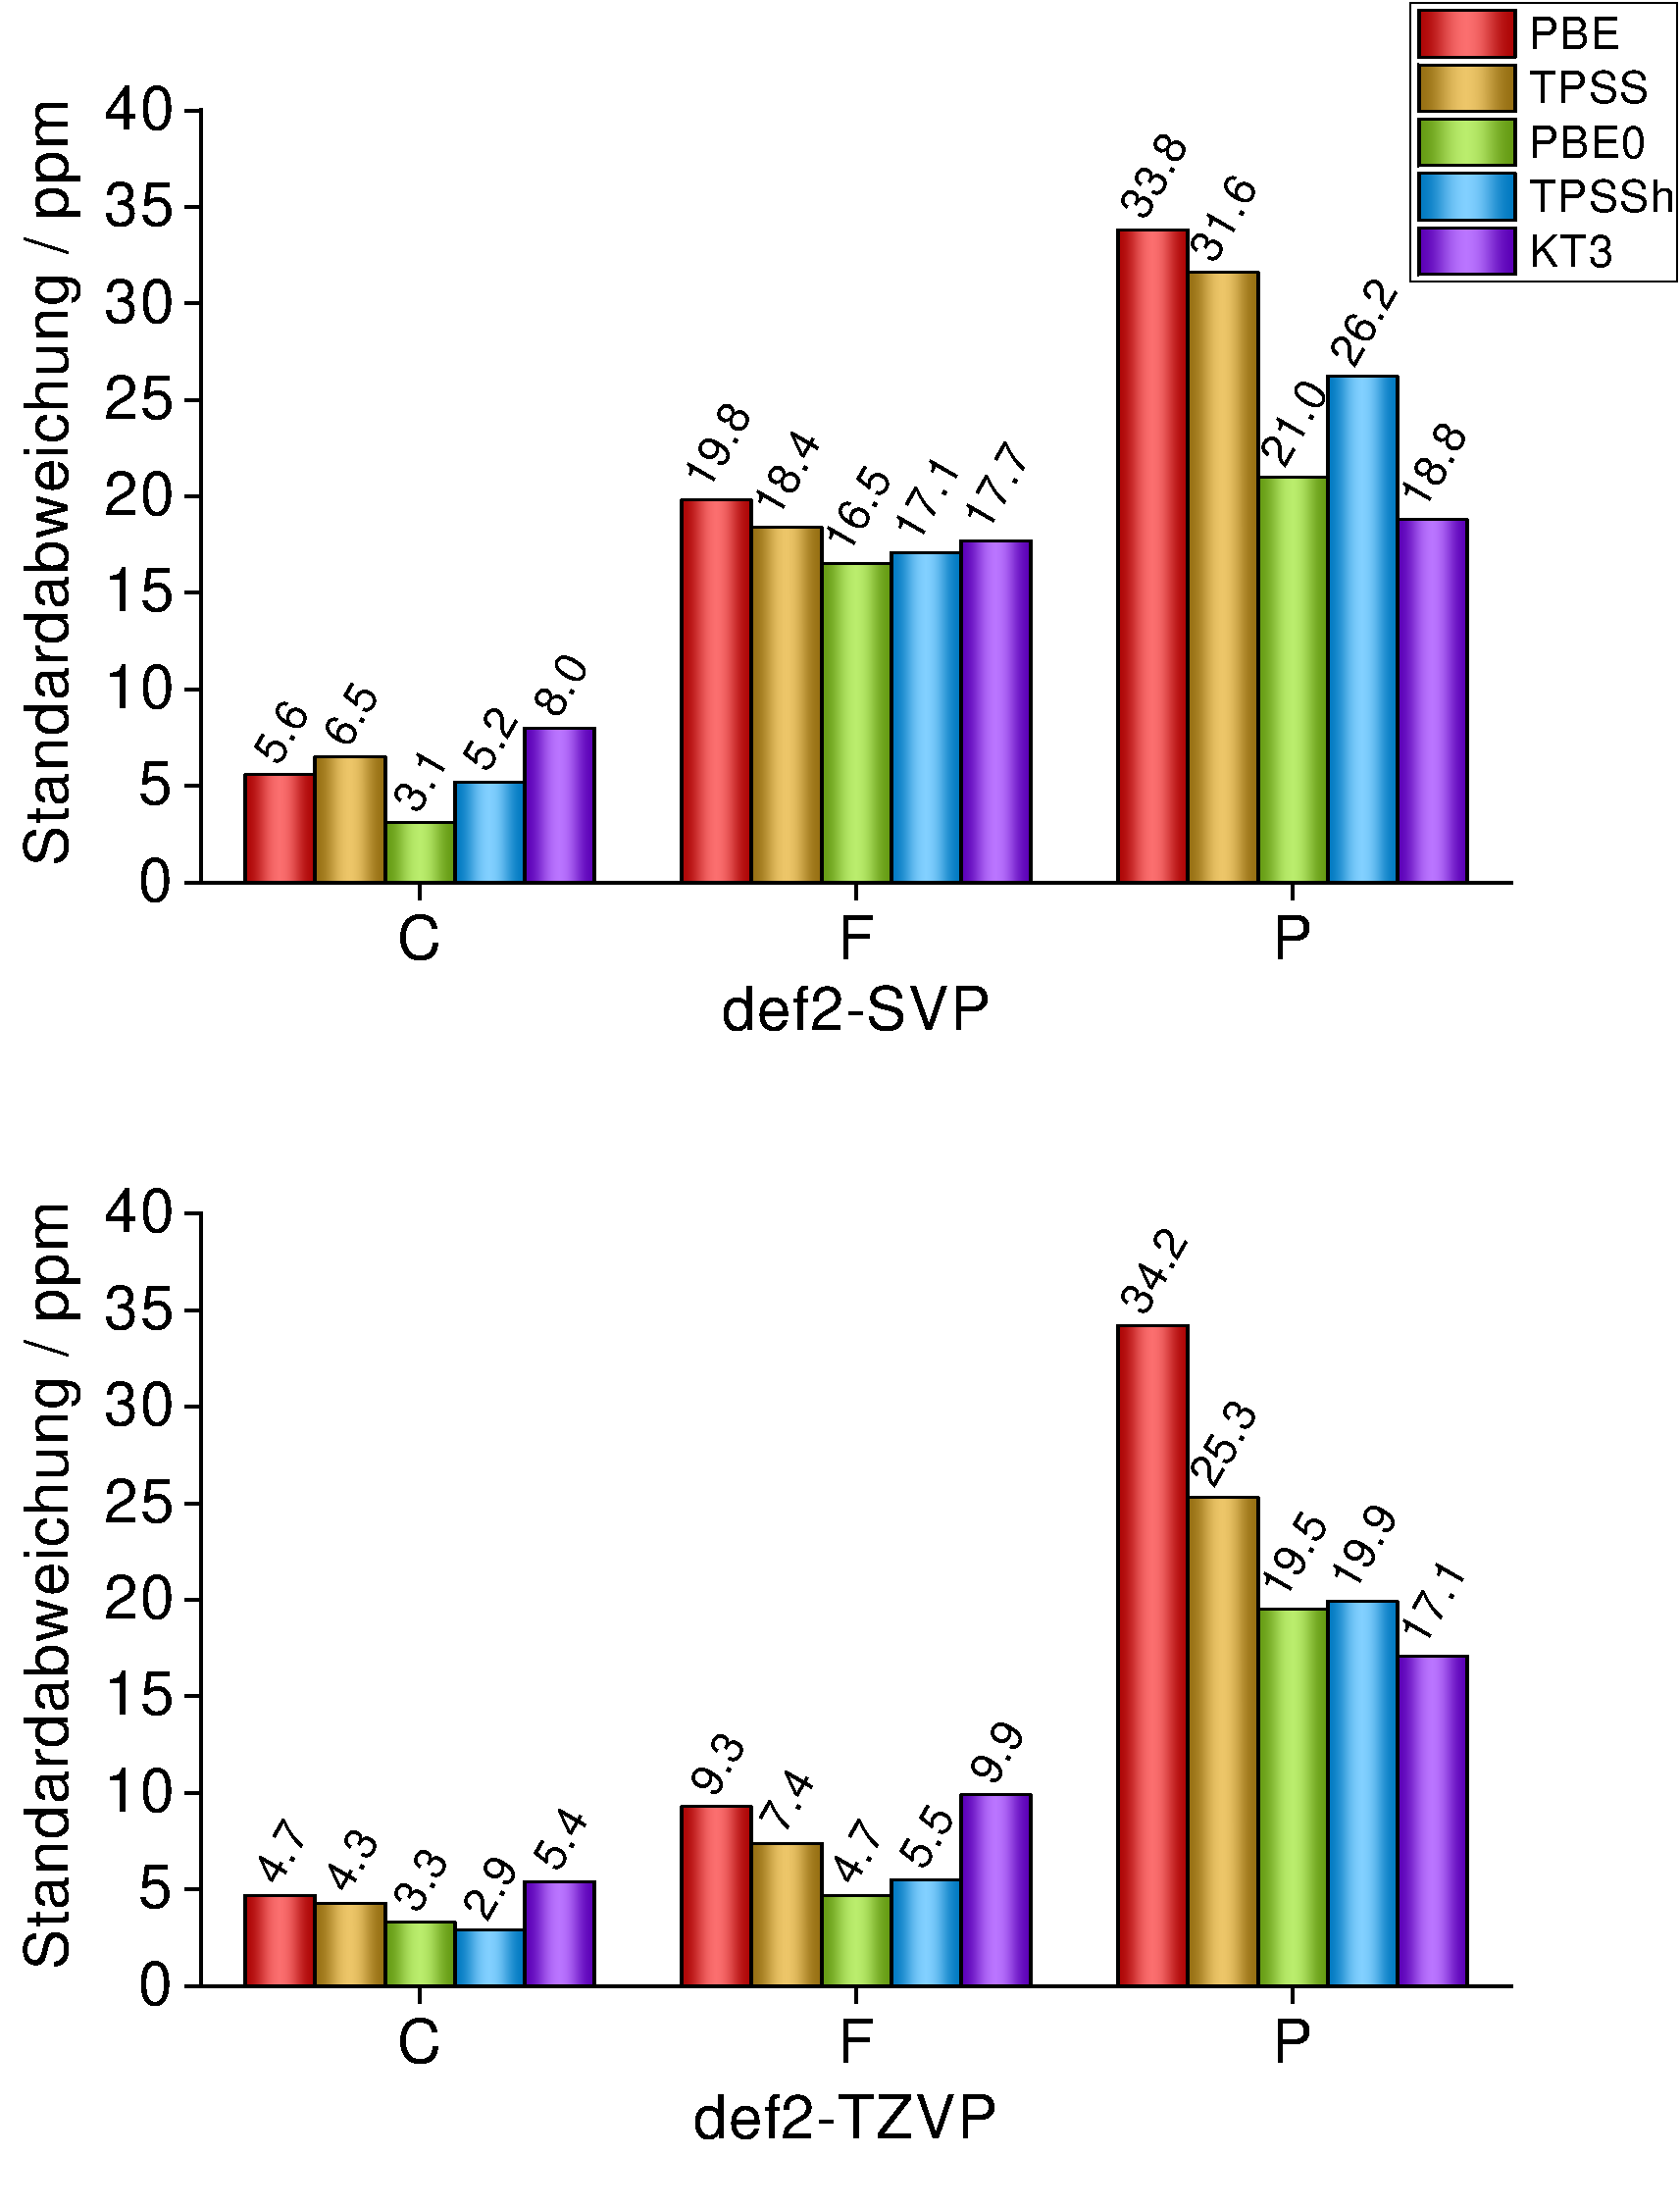
\includegraphics[width=0.72\textwidth]{cfpstd}
	\captionsetup{figurewithin = chapter}
	\captionsetup{font=small, labelfont=bf}\caption[Standardabweichungen für unterschiedliche Funktionale und Basissätze]{Standardabweichungen für C, F und P zwischen gemessenen und berechneten chemischen Verschiebungen in ppm für den Basissatz def2-SVP (oben) und den Basissatz def2-TZVP (unten). Die Verbindungen für die $^{13}$C-chemischen Verschiebungen wurden aus dem Testsatz von Referenz \cite{gauss1993effects} entnommen.} 
\label{abb:cfpshifts}
\end{figure}

\FloatBarrier
Neben den gerade beschriebenen allgemeinen Fehlern, die durch die \ac{dft} gemacht werden, wurden außerdem die zusätzlichen Fehler der in dieser Arbeit implementierten \ac{ri}- und \ac{marij}-Methoden untersucht. Für das \ac{ri}-Verfahren wurden erneut die weiter oben definierten Testsätze für die $^{13}$C-, $^{19}$F- und $^{31}$P-chemischen Verschiebung verwendet und mit den Werten ohne Verwendung der \ac{ri}-Näherung verglichen. Alle Rechnungen wurden unter Verwendung des TPSS-Funktionals und des Basissatzes def2-TZVP durchgeführt. Das \ac{ri}-Verfahren wurde dabei sowohl für die Optimierung der Strukturparameter als auch für die eigentliche Berechnung der chemischen Abschirmungskonstanten angewendet. Im Einzelnen sind die berechneten chemischen Verschiebungen in Tabelle \ref{tab:rierror} aufgelistet. Die Standardabweichung der Differenzen zu den Nicht-\ac{ri}-Rechnungen betragen \unit[0.04]{ppm} für $^{13}$C-chemische Verschiebungen, \unit[0.20]{ppm} für $^{19}$F-chemische Verschiebungen und \unit[0.41]{ppm} für $^{31}$P-chemische Verschiebungen und liegen damit etwa zwei bis drei Größenordnungen unterhalb des Fehlers der \ac{dft}-Rechnung an sich. Für die zusätzliche Beschleunigung durch das \ac{marij}-Verfahren sind die bisher betrachteten Moleküle zu klein, da nur wenige Integrale in den Fernfeld-Bereich fallen und damit durch die Multipolnäherung beschrieben werden würden. Aus diesem Grund wurden mithilfe des SWEET-Programms\supercite{bohne1999sweet} vier Einheiten der $\alpha$-\textsc{d}-Glucose erzeugt. Die kartesischen Koordinaten sowie die entsprechenden chemischen Abschirmungskonstanten sind in Tabelle \ref{tab:marijerror} aufgelistet. Beim Vergleich zischen \ac{ri} und \ac{marij} liegen die statistischen Größen \ac{maa}/\ac{sa}/\ac{maxa} für die $^{13}$C-Abschirmungskonstanten bei \unit[0.004/0.008/0.031]{ppm}, für die $^{1}$H-Abschirmungskonstanten dahingegen nur bei \unit[0.0003/0.0007/0.0038]{ppm}. Die zusätzlichen Fehler, die durch die Multipolnäherung eingeführt werden, sind damit vollkommen vernachlässigbar. Die entsprechenden Größen für den Vergleich zwischen der \ac{ri}- und Nicht-\ac{ri}-Rechnung betragen \unit[0.07/0.26/1.11]{ppm} für $^{13}$C und \unit[0.014/0.019/0.053]{ppm} für $^{1}$H. Auf einem einzelnen Intel\textsuperscript{\textregistered} Xeon\textsuperscript{\textregistered} Prozessor des Typs E5-2687W v2, 3.4 GHz betragen die Rechenzeiten für den Coulombteil \unit[4099]{s} ohne Näherung, \unit[220]{s} mit der \ac{ri}-Näherung und \unit[117]{s} mit der \ac{marij}-Näherung. Die Gesamtrechenzeit für die chemischen Abschirmungskonstanten betragen \unit[4610]{s}, \unit[741]{s} und \unit[633]{s}. Unter Verwendung der \ac{marij}-Methode entspricht dies im vorliegenden Fall einer Beschleunigung um einen Faktor 35 für den Coulombteil bzw. 7 für die gesamte Rechnung ohne einen signifikanten Verlust an Genauigkeit. 

Als weiteres Beispiel wurden die chemischen Abschirmungskonstanten mit dem PBE-Funktional und der Basis def2-SV(P) für ein \aclu*{rns-}\mbox{(\acs{rns}-)}\acused{rns}Segment (2kyd\supercite{2kydstructure}: [C$_{304}$H$_{346}$O$_{220}$N$_{118}$P$_{30}$]$^{30-}$, 10220 Basisfunktionen) berechnet. Die kartesischen Koordinaten wurden der Proteindatenbank entnommen und das System ist in Abbildung \ref{abb:2kyd} gezeigt. Aufgrund der großen negativen Ladung ist die Berechnung nur mithilfe des \ac{cosmo} möglich. Die Rechenzeiten für den Coulombteil betragen \unit[36.2]{h} ohne Näherung, \unit[3.4]{h} mit der \ac{ri}-Näherung und \unit[0.3]{h} mit der \ac{marij}-Näherung. Dies entspricht einer Beschleunigung der Berechnung des Coulombteils um einen Faktor größer als 100. Die Gesamtrechenzeiten betragen \unit[43.2]{h}, \unit[10.7]{h} und \unit[7.6]{h} Stunden, was einem Faktor von etwa 6 auf die Gesamtrechenzeit ergibt. Ein Großteil der verbleibenden Rechenzeit wird für die Berechnung der zahlreichen \ac{cosmo}-Integrale benötigt, wodurch die Beschleunigung der Gesamtrechenzeit hier etwas moderater ausfällt. Jedoch wurde insgesamt, wie auch in den anderen Beispielen, die Zeit für die Berechnung der Wellenfunktion unterboten. Mit der \ac{marij}-Näherung liegt diese bei \unit[9.9]{h}.

\begin{figure}[ht!]
	\centering
	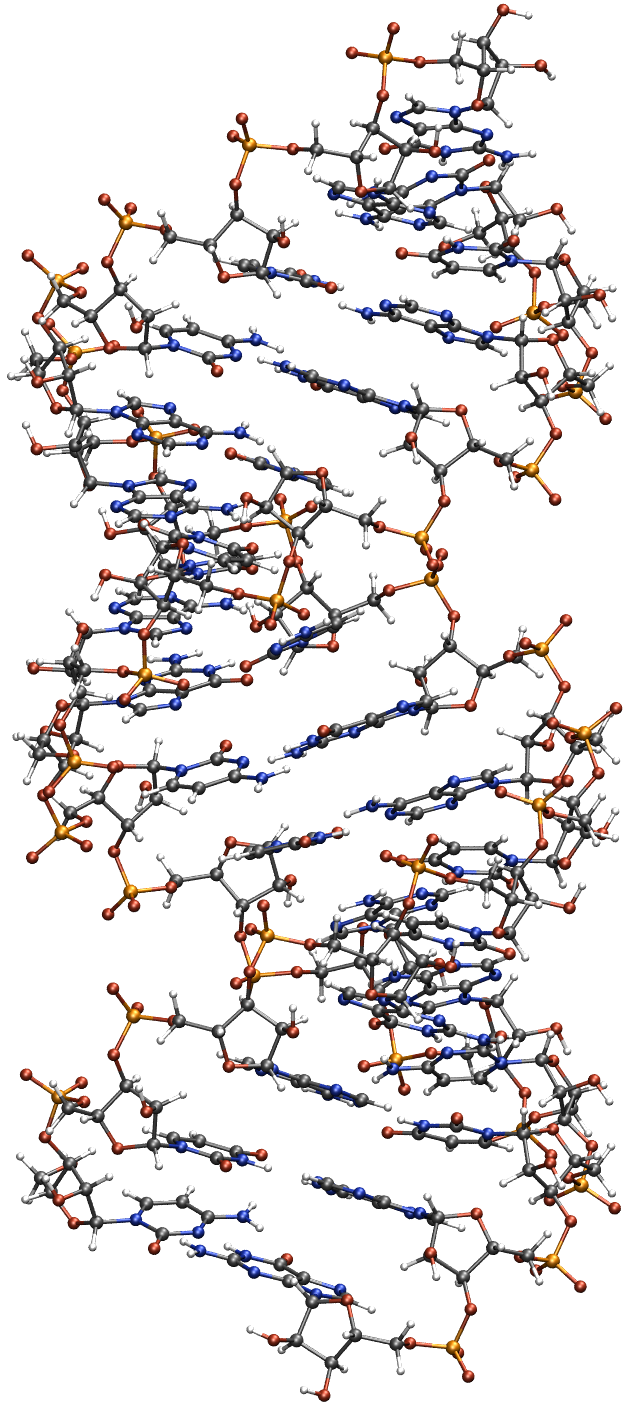
\includegraphics[width=0.6\textwidth]{2kyd}
	\captionsetup{figurewithin = chapter}
	\captionsetup{font=small, labelfont=bf}\caption[{Abbildung eines \ac{rns}-Segmentes}]{Abbildung des \ac{rns}-Segmentes 2kyd\supercite{2kydstructure}: [C$_{304}$H$_{346}$O$_{220}$N$_{118}$P$_{30}$]$^{30-}$ (Kohlenstoff=grau, Wasserstoff=weiß, Sauerstoff=rot, Stickstoff=blau und Phosphor=orange).}
\label{abb:2kyd}
\end{figure}

\bigskip
Neben der Genauigkeit wurde des Weiteren auch die Effizienz der neu implementierten Methoden untersucht. Zunächst wurde dafür das Skalierungsverhalten mit der Molekülgröße für eine gegebene (kleine) Basis betrachtet. Analog zu bisher bestehenden Implementierungen\supercite{beer2011nuclei,kumar2016nuclei} wurden dafür $n$ verknüpfte $\alpha$-\textsc{d}-Glucose-Einheiten mit $n=1,2,4,8,16,32,48,64,128$ betrachtet. Die Strukturen wurden erneut mit dem SWEET-Programm erzeugt. Für die Berechnungen wurde dasselbe Funktional B3LYP\supercite{becke1993density,lee1988development,stephens1994ab} sowie dieselbe Basis/Auxiliarbasis 6-31G$^*$\supercite{hariharan1973influence}/def2-SV(P)\supercite{eichkorn1995auxiliary} verwendet. Zusätzlich wurden noch Berechnungen für die Funktionale PBE, TPSS und TPSSh durchgeführt. Bei allen Berechnungen wurde die Beschleunigung durch die \ac{marij}-Näherung ausgenutzt. Die einzelnen Rechenzeiten auf einem einzelnen Intel\textsuperscript{\textregistered} Xeon\textsuperscript{\textregistered} Prozessor des Typs E5-2687W v2, 3.4 GHz sind in Tabelle \ref{tab:sizeskaling} aufgelistet. 

\begin{table}[ht!]
\centering
\small
\captionsetup{tablewithin = chapter}
\captionsetup{font=small, labelfont=bf}
\captionabove[Rechenzeiten der Abschirmungskonstanten für $n$ verknüpfte $\alpha$-D-Glucose Einheiten]{Rechenzeiten der Abschirmungskonstanten für $n$ verknüpfte $\alpha$-\textsc{d}-Glucose-Einheiten mit unterschiedlichen Funktionalen und dem 6-31G$^*$/def2-SV(P) Basis-/Auxiliarbasissatz. Die Berechnungen wurden auf einem einzelnen Intel\textsuperscript{\textregistered} Xeon\textsuperscript{\textregistered} Prozessor E5-2687W v2, 3.4 GHz durchgeführt. Die Spalten \glqq abs\grqq{} beinhalten absolute Rechenzeiten in Stunden. Für die Hybridfunktionale ist in Klammern die Anzahl der \ac{cphf}-Iterationen angegeben. Die Spalten \glqq rel\grqq{} geben das Verhältnis der Rechenzeit zur vorausgehenden \ac{scf}-Rechnung an. Diese wurden jeweils beginnend mit Hückelorbitalen durchgeführt und konvergierten in 10--17 Iterationen.}
%\resizebox{\textwidth}{!}{%
    \begin{tabular}{S[table-format = 3.0]S[table-format = 2.3]S[table-format = 1.2]S[table-format = 2.3]S[table-format = 1.2]S[table-format = 2.3]@{\hspace{2pt}}rS[table-format = 1.2]S[table-format = 2.3]@{\hspace{5pt}}rS[table-format = 1.2]}
    \hline \hline
          & \multicolumn{2}{c}{PBE} & \multicolumn{2}{c}{TPSS} & \multicolumn{3}{c}{B3LYP} & \multicolumn{3}{c}{TPSSh} \\
    \hline
    $n$     & \text{abs}   & \text{rel}   & \text{abs}   & \text{rel}   & \multicolumn{2}{c}{\text{abs}}   & \text{rel}   & \multicolumn{2}{c}{\text{abs}}   & \text{rel} \\
    1     & 0.003 & 0.75  & 0.005 & 0.83  & 0.009 &(5) & 0.75  & 0.010 &(5) & 0.71 \\
    2     & 0.010 & 0.77  & 0.014 & 0.70  & 0.036 &(7) & 0.76  & 0.035 &(6) & 0.70 \\
    4     & 0.028 & 0.60  & 0.039 & 0.61  & 0.120 &(8) & 0.76  & 0.116 &(6) & 0.71 \\
    8     & 0.079 & 0.60  & 0.103 & 0.65  & 0.389 &(8) & 0.93  & 0.342 &(6) & 0.82 \\
    16    & 0.246 & 0.68  & 0.288 & 0.69  & 1.00 &(9) & 1.00  & 0.914 &(7) & 0.87 \\
    32    & 0.887 & 0.67  & 0.964 & 0.59  & 2.91 &(10) & 1.02  & 2.64 &(7) & 0.92 \\
    48    & 2.00  & 0.55  & 2.15  & 0.49  & 5.75 &(10) & 0.93  & 5.42 &(8) & 0.83 \\
    64    & 3.59  & 0.45  & 3.76  & 0.41  & 10.02 &(10) & 0.83  & 9.48 &(8) & 0.79 \\
    128   & 17.31 & 0.35  & 18.10 & 0.31  & 51.01 &(11) & 0.77  & 42.99 &(8) & 0.66 \\
    \end{tabular}%}%
  \label{tab:sizeskaling}%
\end{table}%

\FloatBarrier

Für das größte System mit $n=128$ (2691 Atome, 23699 Basisfunktionen) kann die Berechnung der chemischen Abschirmungskonstanten auf einer CPU innerhalb eines Tages bzw. zweier Tage bei der Verwendung von reinen bzw. Hybridfunktionalen durchgeführt werden. Für Letztere benötigten die vorausgehenden Berechnungen der Wellenfunktion, welche innerhalb von 10 bis 17 Iterationen konvergierten, etwa genau so viel Zeit wie die eigentlichen Berechnungen der chemischen Abschirmungskonstanten. Tendenziell verbessert sich dieses Verhältnis zugunsten der \ac{nmr}-Rechnung bei großen Systemen. Bei reinen Dichtefunktionalen ohne Hartree-Fock-Austausch ist die Berechnung der Abschirmungskonstanten deutlich schneller als die vorausgehende \ac{scf}-Rechnung. Insgesamt wird für reine Dichteunktionale ein Skalierungsverhalten von $\mathcal{O}(n^{1.8})$ und für Hybridfunktionale ein Skalierungsverhalten von $\mathcal{O}(n^{1.7})$ mit der Systemgröße erhalten. Für die kleineren Systeme bis $n=16$ ist dieses Skalierungsverhalten noch besser. Bei den größeren Systemen beginnen dann $n^3$-Schritte dominant zu werden, was zu einem Skalierungsverhalten von mehr als $\mathcal{O}(n^{2})$ mit der Systemgröße führt. Im Wesentlichen sind das die Diagonalisierung bei der \ac{scf}-Rechnung sowie die Berechnung der Ableitungen nach den Komponenten der Kernmomente für jedes Atom. Die Berechnung für $n=48$ mit dem B3LYP-Funktional, was das größte berechnete System in der bisher aktuellsten Implementierung aus Referenz \cite{kumar2016nuclei} darstellt, benötigt dort \unit[19.8]{h} auf 16 CPUs. Im Vergleich dazu liegt die Rechenzeit mit der in dieser Arbeit vorliegenden Implementierung, wohlgemerkt auf einer CPU, bei weniger als einem Drittel (\unit[5.75]{h}). 

\bigskip
Abgesehen von der bisherigen Betrachtung des Skalierungsverhaltens beim Vergrößern der Systemgröße, wurde auch der Einfluss einer größeren Basis bei gleicher Systemgröße untersucht. Für das System mit $n=16$ wurde daher die Basis def2-TZVP verwendet, welche etwa 2.5 mal so groß wie die bisher betrachtete Basis 6-31G$^*$ ist. Bei der Verwendung des TPSS-Funktionals führt dies zu einer Verlängerung der Rechenzeit für die Abschirmungskonstanten um einen Faktor von ca. 4.6 und damit zu einem Skalierungsverhalten von $\mathcal{O}(n^{1.7})$ ($\frac{\log(4.6)}{\log(2.5)}$). Die Berechnung mit dem Hybridfunktional TPSSh führt zu einer Verlängerung um einen Faktor von ca. 19 und damit zu einem deutlich weniger guten Skalierungsverhalten von etwa $\mathcal{O}(n^{3.2})$. Dies kann dadurch begründet werden, dass durch die größere Basis im Wesentlichen Funktionen mit größerer $l$-Quantenzahl hinzugefügt werden. Deren Beiträge können zum großen Teil nicht bei der Integralabschätzung vernachlässigt werden, wodurch das eigentliche Skalierungsverhalten nicht weit vom formalen Skalierungsverhalten mit $\mathcal{O}(n^{4})$ entfernt liegt. Abhilfe lässt sich möglicherweise durch die Implementierung der \ac{ri}-Methode für den Austausch, \ac{ri}-\textit{K}\supercite{weigend2002fully}, oder durch seminumerische Berechnung\supercite{neese2009efficient,plessow2012seminumerical} des Letzteren schaffen. Die parallele Ausführung des Programms auf 4 CPUs führt für das System mit $n=32$ und der Basis 6-31G$^*$ zu einer Beschleunigung der Berechnung um einen Faktor von ca. 3.1, für das System mit $n=16$ und der Basis def2-TZVP zu einer Beschleunigung um einen Faktor von ca. 3.6. Dies trifft sowohl auf die Verwendung reiner \ac{dft}-Funktionale als auch auf Hybridfunktionale zu.


\chapter{Anwendungen}\label{anwendungen}
Die in dieser Arbeit vorgestellten Methoden wurden auf reale chemische Fragestellungen angewendet um die experimentellen Befunde zu unterstützen bzw. besser deuten zu können.
Im ersten Abschnitt dieses Kapitels wird die Anwendung auf eine Reihe anorganischer Verbindungen beschrieben. Der zweite Abschnitt widmet sich der Untersuchung von Ringströmen in großen Kohlenstoff Nanoröhren wofür die gestörte Elektronendichte benötigt wird. Durch die in dieser Arbeit implementierten Methoden zur Verbesserung der Effizienz wurde die Berechnung dieser gestörten Dichtematrix in einem akzeptablen Zeitrahmen ermöglicht. 

\section{Anwendungen in der anorganischen Chemie}
\FloatBarrier
\subsection{\texorpdfstring{$^{31}$P}{31P} chemische Verschiebungen in Phospor NHCs}
Um ein besseres Verständnis der chemischen Verschiebung in einer Reihe von Phosphor-N-Heterocyclischen-Carben-(\acs{nhc}) Verbindungen \supercite{lemp2017nhc} zu erhalten, wurden die chemischen Abschirmungskonstanten für die in den Abbildung \ref{abb:cvh1} bis \ref{abb:cvh7} gezeigten Verbindungen auf \ac{dft} Niveau berechnet. Die in Tabelle \ref{tab:cvhtab1} gelisteten Werte wurden unter Verwendung des PBE Funktionals\supercite{perdew1996generalized} und des def2-TZVP Basissatzes\supercite{weigend2005balanced} erhalten. Zuvor wurden die Strukturparameter der entsprechenden Verbindungen auf dem selben Niveau optimiert, wobei zusätzlich Grimmes Dispersionskorrektur D3\supercite{grimme2010consistent} verwendet wurde. Weiterhin wurde das \ac{cosmo}\supercite{klamt1993cosmo} mit einer Dielektrizitätskonstante von 2.28 verwendet um das experimentelle Lösungsmittel Benzol zu simulieren. Zusätzlich zu den berechneten absoluten Abschirmungskonstanten sind in Tabelle \ref{tab:cvhtab1} sowohl die experimentellen $^{31}$P und $^{13}C$ (Carbenkohlenstoff) Verschiebungen als auch simulierte chemische Verschiebungen aus den berechneten Werten angegeben: $\delta=\sigma_0-\sigma$. $\sigma_0$ wurde durch Minimieren der Abweichung zwischen den experimentellen Verschiebungen und berechneten Abschirmungen bestimmt. Für die $^{13}C$ Verschiebungen wird damit eine Übereinstimmung zwischen Experiment und Rechnung bis auf etwa \unit[2]{ppm} erhalten und die Reihenfolge korrekt wiedergegeben. Die $^{31}$P Verschiebungen sind aufgrund ihres größeren Bereichs der chemischen Verschiebung deutlich problematischer. Fehler von \unit[30]{ppm} sind keine Seltenheit, wie bereits gezeigt wurde.\supercite{latypov2015quantum,reiter2017calculation} Abgesehen von der Verbindung $[$SIMesPGa\textit{t}Bu$_2]_2$ liegen die anderen Verbindungen damit also in einem akzeptablen Bereich. Die Trends in der $^{31}$P Verschiebung werden korrekt wiedergegeben und auch die vergleichsweise niedrige Abschirmung in K(SIMesP)$_3$Al\textit{t}Bu wird durch die Berechnung bestätigt. Diese Befunde sind vom verwendeten Funktional unabhängig wie Tabelle \ref{tab:cvhtab2} zeigt. Neben den berechneten Werten mit dem PBE Funktional, sind dort auch die Ergebnisse mit den Funktionalen PBE0\supercite{adamo1999toward}, BP86\supercite{perdew1986density,becke1988density} und B3LYP\supercite{becke1993density,lee1988development,stephens1994ab} sowie einer Hartree-Fock-Rechnung aufgelistet. Grundlage für diese Berechnungen waren jedoch die experimentellen Strukturen.

\begin{table}[ht!]
\captionsetup{tablewithin = chapter}
\captionsetup{font=small, labelfont=bf}
\captionabove[Vergleich spektroskopischer und struktureller Daten für Phosphor \acp{nhc}]{Vergleich spektroskopischer und struktureller Daten für SIMesPH, IMesPH, $[$SIMesPGa\textit{t}Bu$_2]_2$, SIMesP(Ga\textit{t}Bu$_2$)$_2$Cl, K(SIMesP)$_3$Al\textit{t}Bu, SIMesPH\textit{t}Bu$_2$GaCl und SIMesPH\textit{t}Bu$_2$AlCl.}
\resizebox{\textwidth}{!}{%
\begin{tabular}{ccccccccc}
\hline \hline
Verbindung & \multicolumn{3}{c}{$^{31}$P / ppm} & \multicolumn{3}{c}{$^{13}$C (Carbenkohlenstoff) / ppm} & \multicolumn{2}{c}{P-C Abstand/ pm}\\
 & gemessen & \multicolumn{2}{c}{berechnet} & gemessen & \multicolumn{2}{c}{berechnet} &Röntgenstruktur & berechnet\\
 & & sim. $\delta ^{31}$P & $\sigma ^{31}$P & & sim. $\delta ^{13}$C & $\sigma ^{13}$C & & \\
 \hline
 SIMesPH & -127.2 & -157 & 433 & 191.0 & 192 & -3 & 174.6(2) & 175.3\\
 IMesPH & -147.3 & -178 & 454 & 180.0 & 178 & 11 & 174.7(2) & 176.1\\
 $[$SIMesPGa\textit{t}Bu$_2]_2$ & -113.2 & -57 & 333 & & 182 & 7 & 174.4(2) & 175.6\\
 SIMesP(Ga\textit{t}Bu$_2$)$_2$Cl & -122.6 & -104 & 380 & 183.3 & 181 & 8 & 175.4(1) & 175.3\\
 K(SIMesP)$_3$Al\textit{t}Bu & -61.2 & -54 & 330 & & 185 & 4 & 175.3(2) & 175.8\\
 SIMesPH\textit{t}Bu$_2$GaCl & -148.8 & -163 & 439 & 188.5 & 191 & -2 & 179.8(2) & 179.4\\
 SIMesPH\textit{t}Bu$_2$AlCl & -151.0 & -157 & 433 & 187.9 & 190 & -1 & 180.1(2) & 179.5
\end{tabular}}
\label{tab:cvhtab1}
\end{table}

\begin{table}[ht!]
\captionsetup{tablewithin = chapter}
\captionsetup{font=small, labelfont=bf}
\captionabove[$^{31}$P Verschiebungen/Abschirmungen für Phosphor \acp{nhc} mit unterschiedlichen Funktionalen]{$^{31}$P Verschiebungen/Abschirmungen für SIMesPH, IMesPH, $[$SIMesPGa\textit{t}Bu$_2]_2$, SIMesP(Ga\textit{t}Bu$_2$)$_2$Cl, K(SIMesP)$_3$Al\textit{t}Bu, SIMesPH\textit{t}Bu$_2$GaCl und SIMesPH\textit{t}Bu$_2$AlCl mit unterschiedlichen Funktionalen. Die Spalte \glqq PBE, opt\grqq{} enthält die berechneten Werte für optimierte Strukturparameter. Alle Werte in den darauf folgenden Spalten wurden auf Grundlage der experimentellen Strukturparametern berechnet. Alle Werte sind in ppm angegeben.}
\resizebox{\textwidth}{!}{%
\begin{tabular}{cccccccccccccc}
\hline \hline
Verbindung &gemessen &\multicolumn{2}{c}{PBE, opt} &\multicolumn{2}{c}{PBE} &\multicolumn{2}{c}{BP86} &\multicolumn{2}{c}{B3-LYP} &\multicolumn{2}{c}{PBE0} &\multicolumn{2}{c}{HF}\\
& & $\delta ^{31}$P & $\sigma ^{31}$P & $\delta ^{31}$P & $\sigma ^{31}$P & $\delta ^{31}$P & $\sigma ^{31}$P & $\delta ^{31}$P & $\sigma ^{31}$P & $\delta ^{31}$P & $\sigma ^{31}$P & $\delta ^{31}$P & $\sigma ^{31}$P\\
\hline
SIMesPH &-127,2 &-157 &433 &-164 &455 &-165 &450 &-163 &443 &-155 &465 &-140 &491\\
IMesPH &-147,3 &-178 &454 &-137 &428 &-138 &423 &-136 &416 &-133 &443 &-121 &472\\
$[$SIMesPGa\textit{t}Bu$_2]_2$ &-113,2 &-57  &333 &-59  &350 &-58  &343 &-61  &341 &-68  &378 &-94  &445\\
SIMesP(Ga\textit{t}Bu$_2$)$_2$Cl &-122,6 &-104 &380 &-109 &400 &-107 &392 &-111 &391 &-117 &427 &-137 &488\\
K(SIMesP)$_3$Al\textit{t}Bu &-61,2  &-54  &330 &-77  &368 &-77  &362 &-79  &359 &-83  &393 &-99  &450\\
SIMesPH\textit{t}Bu$_2$GaCl &-148,8 &-163 &439 &-162 &453 &-162 &447 &-162 &442 &-160 &470 &-144 &495\\
SIMesPH\textit{t}Bu$_2$AlCl &-151   &-157 &433 &-163 &454 &-164 &449 &-161 &441 &-158 &468 &-137 &488\\
\end{tabular}}
\label{tab:cvhtab2}
\end{table}

\FloatBarrier

Bei genauerer Betrachtung der Berechnungen hat sich herausgestellt, dass die Unterschiede in den chemischen Abschirmungskonstanten der einzelnen Verbindungen im Wesentlichen aufgrund des paramagnetischen Beitrages zustande kommen. In diesem Beitrag ist die Response der Elektronendichte auf das äußere Magnetfeld enthalten, im diamagnetischen Beitrag hingegen die Elektronendichte selbst. Erwartungsgemäß ist der diamagnetische Beitrag in allen untersuchten Verbindungen sehr ähnlich und liegt zwischen \unit[960]{ppm} und \unit[967]{ppm}. Dieser Befund führt zu der Schlussfolgerung, dass alle weiteren Untersuchungen, welche auf der Elektronendichte basieren (wie beispielsweise Populationsanalysen), nicht dafür geeignet sind die Unterschiede in den einzelnen Abschirmungskonstanten zu erklären. Eine erhöhte Elektronendichte und eine damit einhergehende stärker negative Partialladung am Phosphoratom führt also nicht zwangsläufig zu einer stärkeren Abschirmung. Der paramagnetische Beitrag hingegen ist anfällig auf Änderungen in der Geometrie und der elektronischen Struktur der jeweiligen Verbindung. Dies wird beispielsweise beim Vergleich von SIMesPH und IMesPH deutlich, welche eine chemische Verschiebung von etwa \unit[20]{ppm} zueinander aufweisen. Die beiden Strukturen unterscheiden sich lediglich durch die Anzahl der Wasserstoffatome an den Kohlenstoffatomen im fünfgliedrigen Ring. Die große Änderung der elektronischen Struktur wird auch bei der Rotation der C-P Bindung offensichtlich. Die $^{31}$P Abschirmungskonstante in den jeweiligen Übergangszuständen liegt um ca. \unit[60]{ppm} höher als die des zugehörigen Grundzustandes. Um den rein elektronischen Einfluss auf die Abschirmungskonstanten der Grundzustände von SIMesPH und IMesPH weiter zu untersuchen, wurde in der Verbindung SIMesPH jeweils ein Wasserstoffatom an den Kohlenstoffatomen entfernt und die Positionen aller anderen Atome beibehalten. Die erhaltene Abschirmungskonstante liegt bei etwa \unit[444]{ppm} und damit genau in der Mitte der beiden Verbindungen. All diese Unterschiede basieren allein auf dem paramagnetischen Beitrag. Der diamagnetische Beitrag liegt in allen Fällen bei \unit[962]{ppm}.
Diese hohe Sensibilität mag der ausschlaggebende Grund für den Unterschied zwischen der experimentellen und berechneten chemischen Verschiebung in $[$SIMesPGa\textit{t}Bu$_2]_2$ sein. Diese Verbindung unterscheidet sich von SIMesP(Ga\textit{t}Bu$_2$)$_2$Cl nur durch das Ersetzen eines SIMesP-Restes durch ein Chloratom. Wird erneut die Geometrie von $[$SIMesPGa\textit{t}Bu$_2]_2$ genommen und dieser Austausch durchgeführt, so wird bei der Nachoptimierung der Position des Chloratoms unter Beibehaltung der restlichen Strukturparameter eine 
$^{31}$P Abschirmungskonstante von \unit[336]{ppm} erhalten. Dieser Wert ist fast identisch mit dem aus der Verbindung $[$SIMesPGa\textit{t}Bu$_2]_2$ und unterscheidet sich daher deutlich vom Wert der Verbindung mit optimierten Strukturparametern (SIMesP(Ga\textit{t}Bu$_2$)$_2$Cl, \unit[380]{ppm}). Die Änderung der Strukturparameter hat daher eindeutig einen großen Einfluss auf den paramagnetischen Beitrag. Die Ähnlichkeit in der gemessenen Abschirmung von $[$SIMesPGa\textit{t}Bu$_2]_2$ und SIMesP(Ga\textit{t}Bu$_2$)$_2$Cl ist daher überraschender als die vergleichsweise kleine gemessene und berechnete Verschiebung in der Verbindung K(SIMesP)$_3$Al\textit{t}Bu.
Zur weiteren Untersuchung dieser Erkenntnisse wurde eine Zerlegung des diamagnetischen und paramagnetischen Teils der chemischen Abschirmungskonstante in einzelne Orbitalbeiträge exemplarisch für SIMesP(Ga\textit{t}Bu$_2$)$_2$Cl unternommen wie es beispielsweise von Wiberg \textit{et al.}\supercite{wiberg1998nmr} vorgeschlagen wurde. Im Detail sind die Werte in Tabelle \ref{tab:cvhzerlegung} im Anhang zu finden. Zusätzlich sind dort in Abbildung \ref{abb:modec} die \acp{mo} gezeigt, welche den größten Beitrag liefern. Erwartungsgemäß dominieren die inneren Orbitale des Phosphoratoms den diamagnetischen Beitrag. Hauptsächlich sind dies das 1s mit ca. \unit[500]{ppm} aber auch die 2s und 2p Orbitale, welche jeweils einen Beitrag von ca. \unit[100]{ppm} liefern. Der größte Beitrag für den paramagnetischen Anteil kommt mit ca. \unit[-180]{ppm} von der c-P $\pi$-Bindung. Allerdings gibt es viele Orbitale welche ebenfalls einen Beitrag von mehr als \unit[10]{ppm} liefern. Die vergleichsweise kleinen Unterschiede in der chemischen Abschirmung der untersuchten Verbindungen lassen sich damit daher nicht weiter auflösen.

\begin{figure}[ht!]
	\centering
	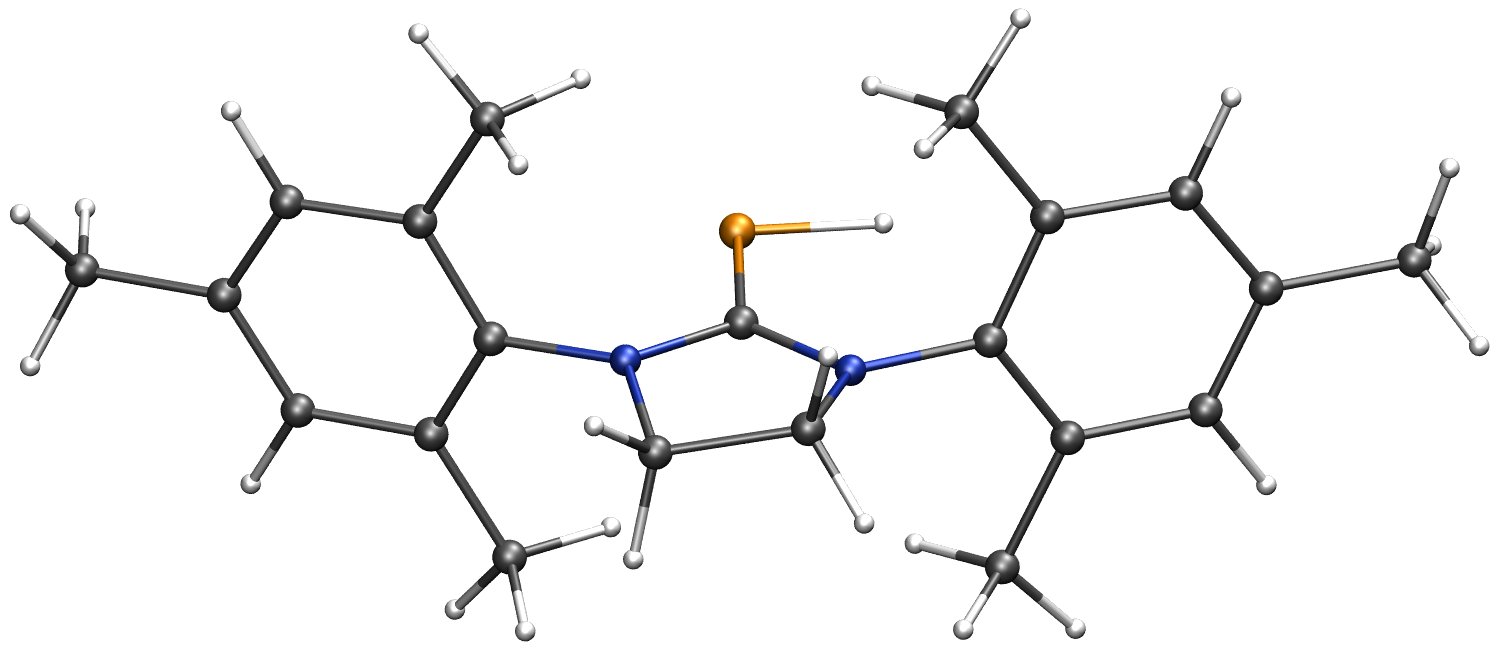
\includegraphics[width=0.6\textwidth]{1}
	\captionsetup{figurewithin = chapter}
	\captionsetup{font=small, labelfont=bf}\caption[Abbildung von SIMesPH]{Abbildung von SIMesPH, SIMes=1,3-bis(2,4,6-tri\-me\-thyl\-phe\-nyl)imi\-da\-zo\-lin-2-yli\-den (Kohlenstoff=grau, Wasserstoff=weiß, Stickstoff=blau und Phosphor=orange).}
\label{abb:cvh1}
\end{figure}

\begin{figure}[ht!]
	\centering
	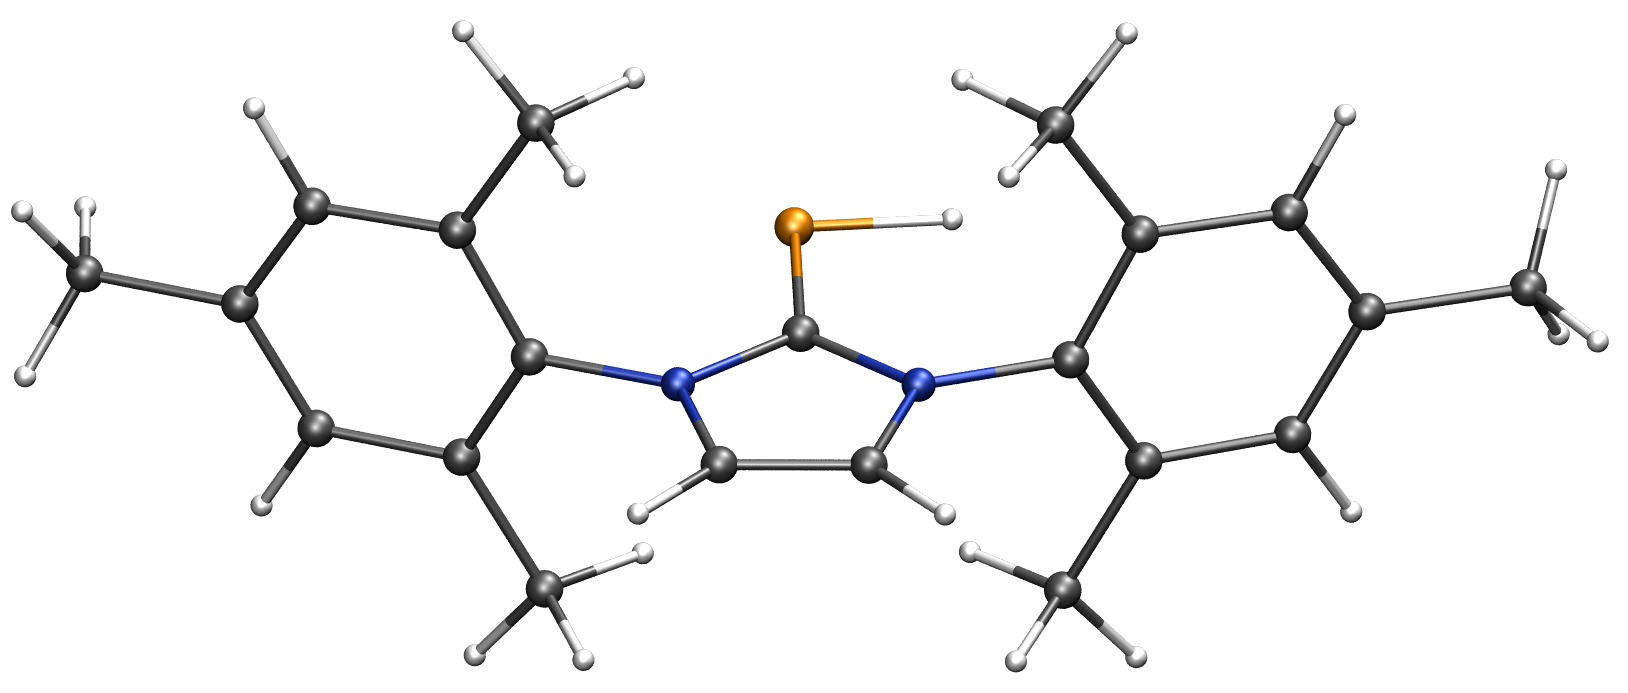
\includegraphics[width=0.6\textwidth]{2}
	\captionsetup{figurewithin = chapter}
	\captionsetup{font=small, labelfont=bf}\caption[Abbildung von IMesPH]{Abbildung von IMesPH, IMes=1,3-bis(2,4,6-tri\-me\-thyl\-phe\-nyl)imi\-da\-zol-2-yli\-den (Kohlenstoff=grau, Wasserstoff=weiß, Stickstoff=blau und Phosphor=orange).}
\label{abb:cvh2}
\end{figure}

\begin{figure}[ht!]
	\centering
	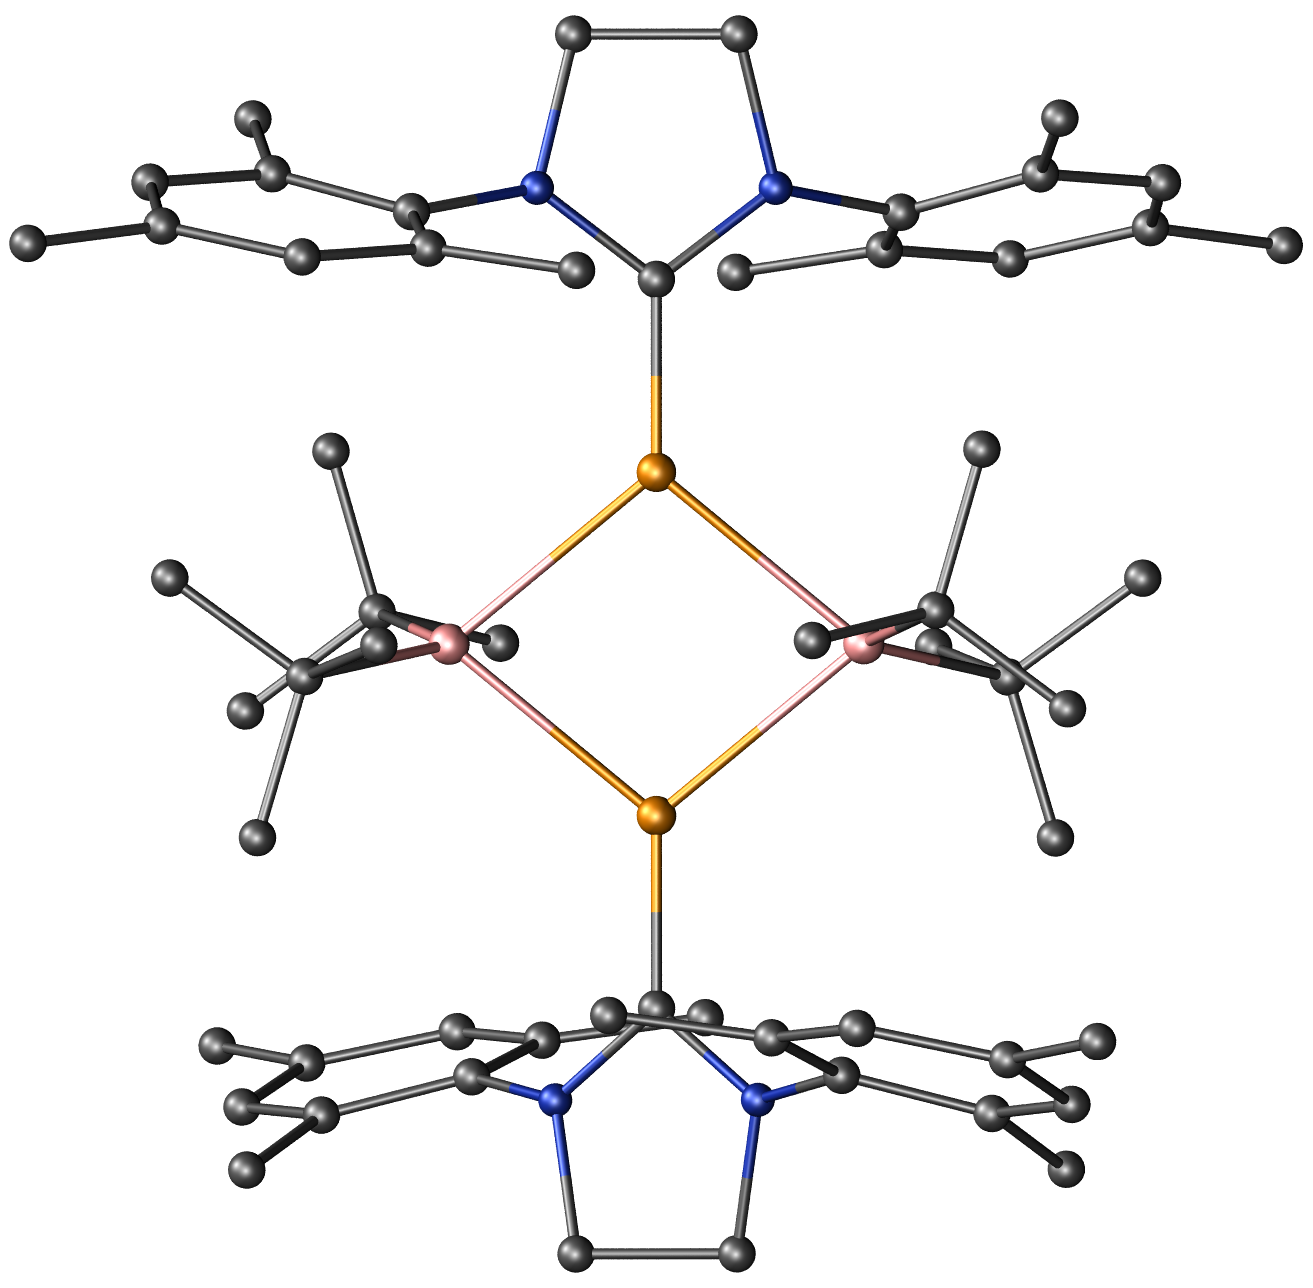
\includegraphics[width=0.6\textwidth]{3}
	\captionsetup{figurewithin = chapter}
	\captionsetup{font=small, labelfont=bf}\caption[{Abbildung von $[$SIMesPGa\textit{t}Bu$_2]_2$}]{Abbildung von $[$SIMesPGa\textit{t}Bu$_2]_2$, SIMes=1,3-bis(2,4,6-tri\-me\-thyl\-phe\-nyl)imi\-da\-zo\-lin-2-yli\-den (Kohlenstoff=grau, Stickstoff=blau, Phosphor=orange und Gallium=rosa). Die Wasserstoffatome wurden zur besseren Veranschaulichung bei der Abbildung weg gelassen.}
\label{abb:cvh3}
\end{figure}

\begin{figure}[ht!]
	\centering
	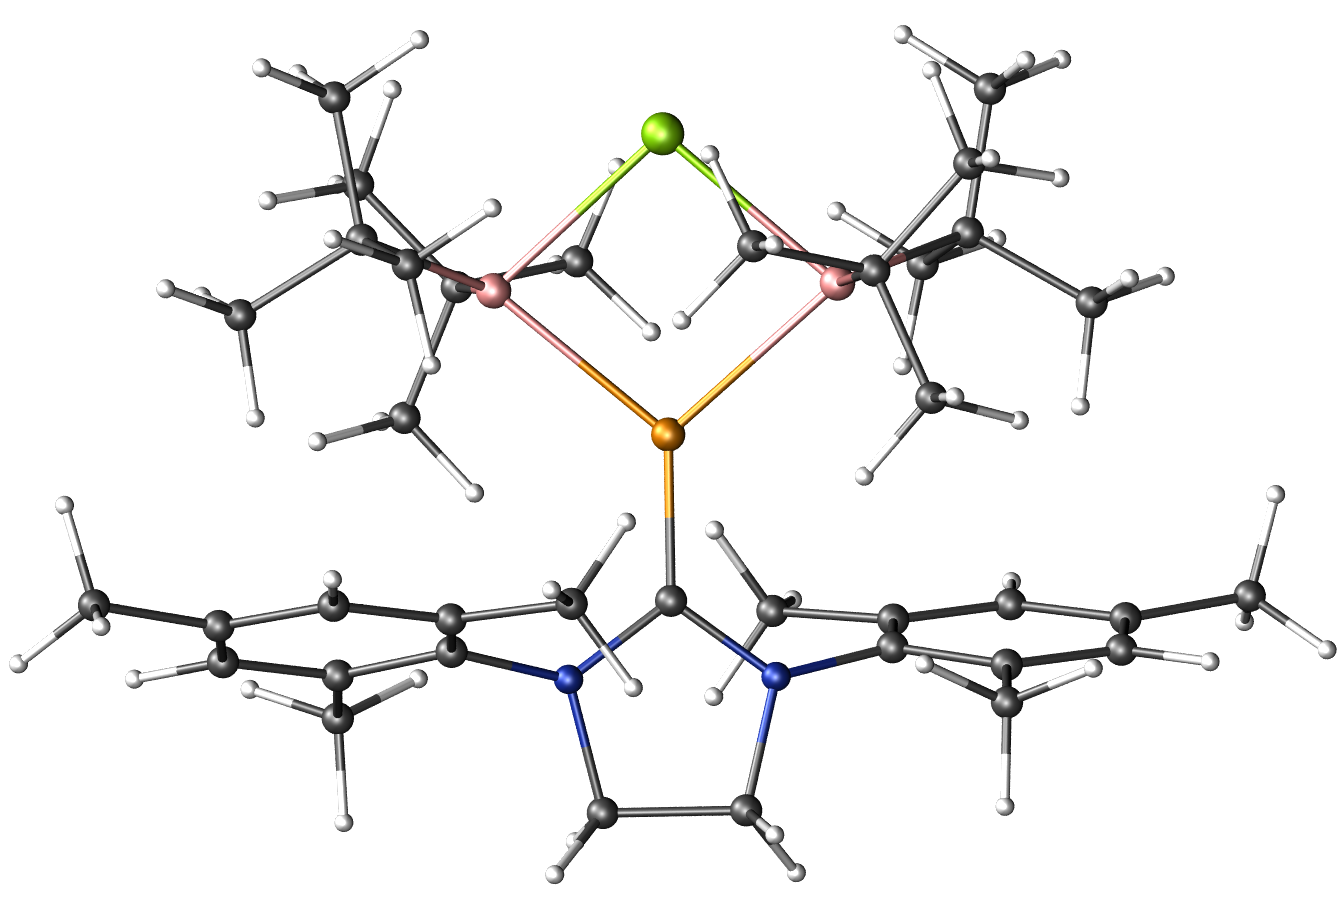
\includegraphics[width=0.6\textwidth]{4}
	\captionsetup{figurewithin = chapter}
	\captionsetup{font=small, labelfont=bf}\caption[Abbildung von SIMesP(Ga\textit{t}Bu$_2$)$_2$Cl]{Abbildung von SIMesP(Ga\textit{t}Bu$_2$)$_2$Cl, SIMes=1,3-bis(2,4,6-tri\-me\-thyl\-phe\-nyl)imi\-da\-zo\-lin-2-yli\-den (Kohlenstoff=grau, Wasserstoff=weiß, Stickstoff=blau, Phosphor=orange, Gallium=rosa und Chlor=grün).}
\label{abb:cvh4}
\end{figure}

\begin{figure}[ht!]
	\centering
	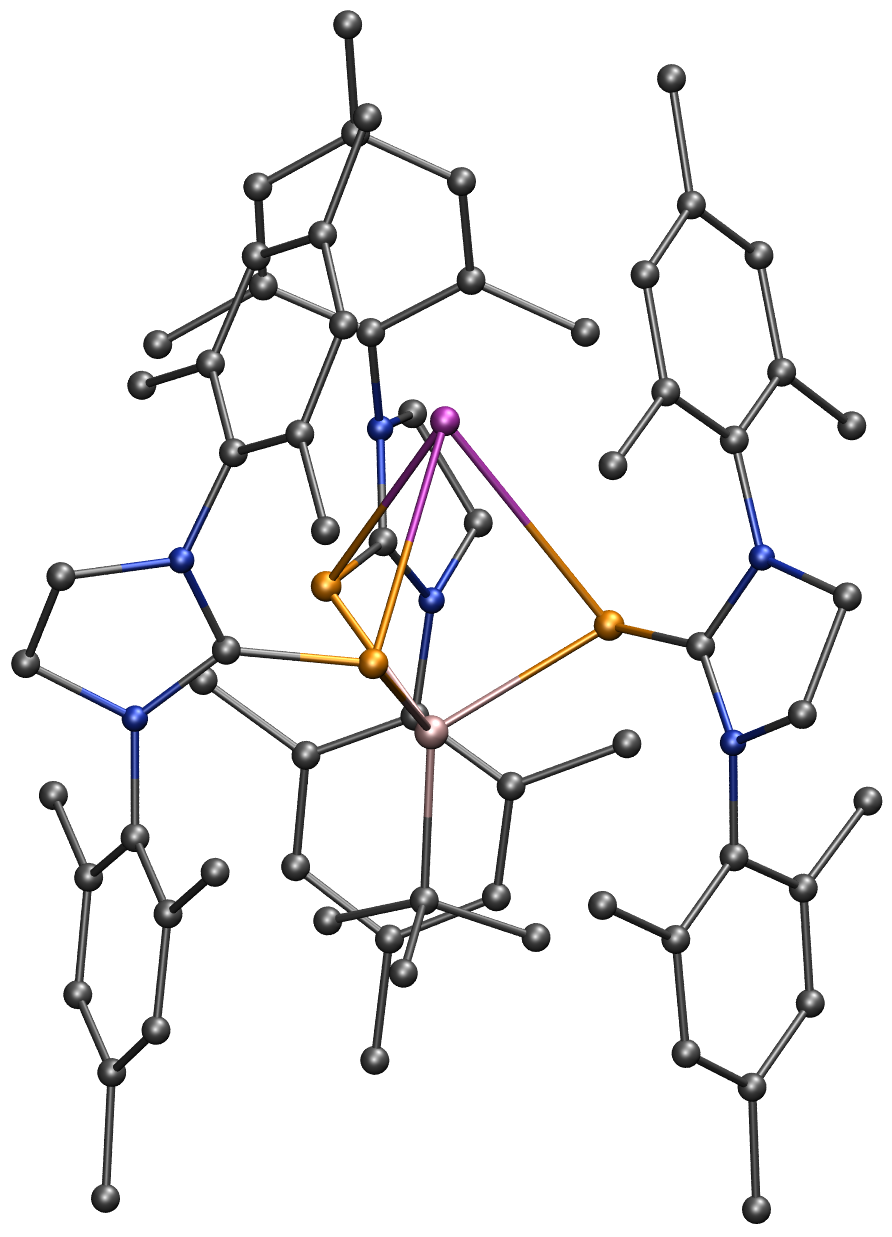
\includegraphics[width=0.5\textwidth]{5}
	\captionsetup{figurewithin = chapter}
	\captionsetup{font=small, labelfont=bf}\caption[Abbildung von K(SIMesP)$_3$Al\textit{t}Bu]{Abbildung von K(SIMesP)$_3$Al\textit{t}Bu, SIMes=1,3-bis(2,4,6-tri\-me\-thyl\-phe\-nyl)imi\-da\-zo\-lin-2-yli\-den (Kohlenstoff=grau, Stickstoff=blau, Phosphor=orange, Kalium=lila und Aluminium=hellrosa). Die Wasserstoffatome wurden zur besseren Veranschaulichung bei der Abbildung weg gelassen.}
\label{abb:cvh5}
\end{figure}

\begin{figure}[ht!]
	\centering
	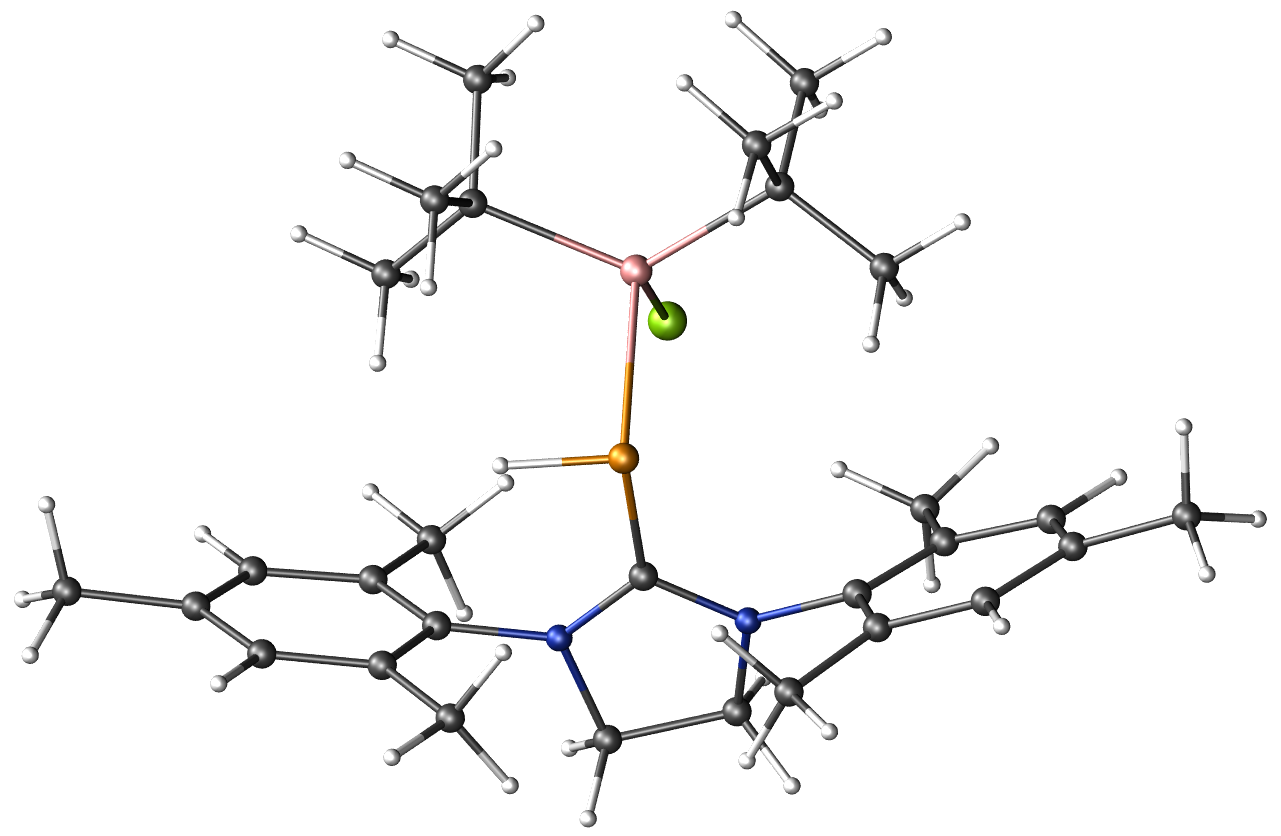
\includegraphics[width=0.6\textwidth]{6}
	\captionsetup{figurewithin = chapter}
	\captionsetup{font=small, labelfont=bf}\caption[Abbildung von SIMesPH\textit{t}Bu$_2$GaCl]{Abbildung von SIMesPH\textit{t}Bu$_2$GaCl, SIMes=1,3-bis(2,4,6-tri\-me\-thyl\-phe\-nyl)imi\-da\-zo\-lin-2-yli\-den (Kohlenstoff=grau, Wasserstoff=weiß, Stickstoff=blau, Phosphor=orange, Gallium=rosa und Chlor=grün).}
\label{abb:cvh6}
\end{figure}

\begin{figure}[ht!]
	\centering
	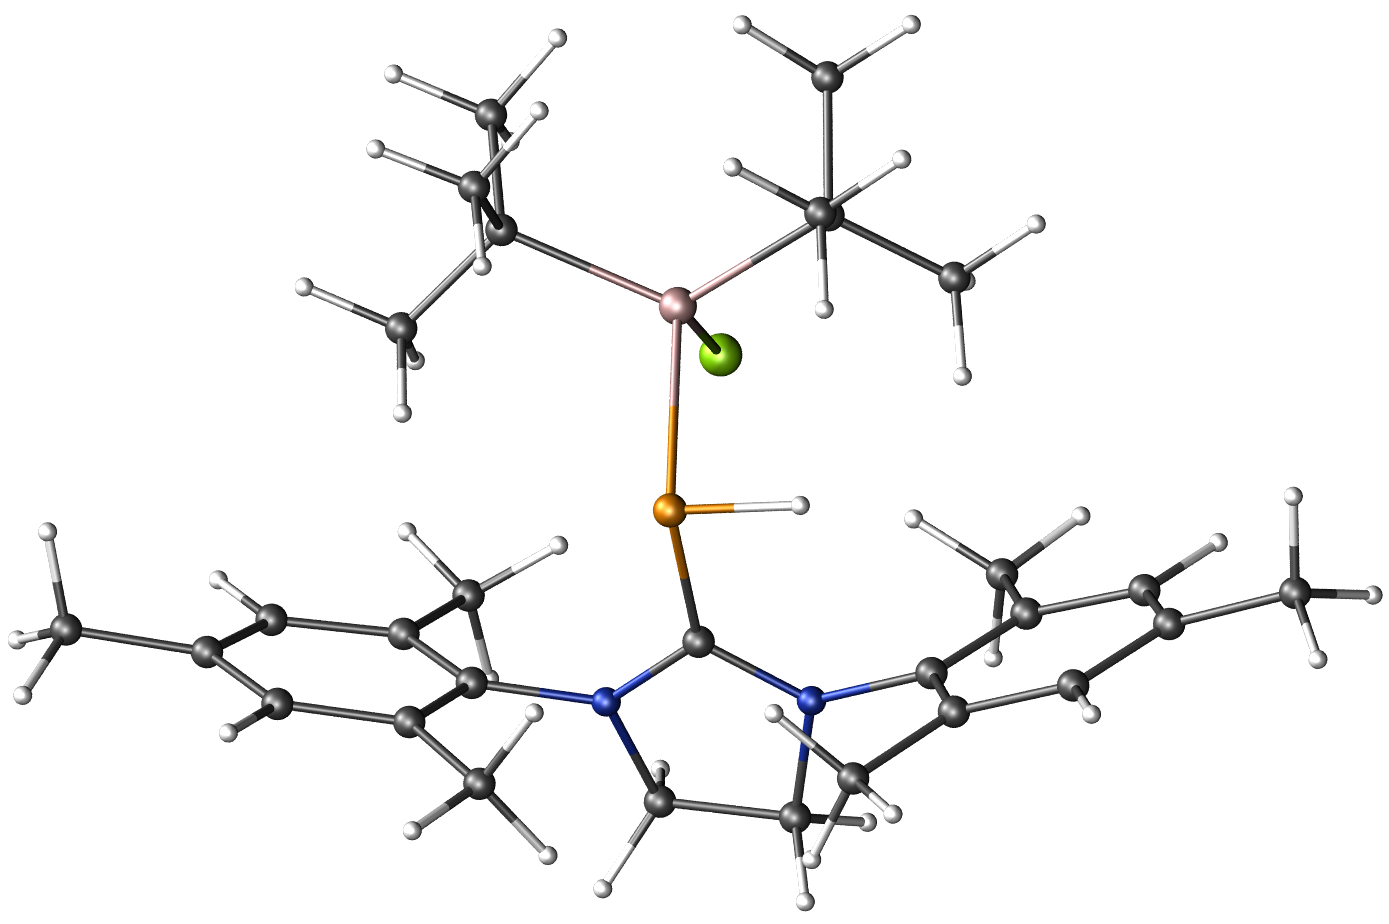
\includegraphics[width=0.6\textwidth]{7}
	\captionsetup{figurewithin = chapter}
	\captionsetup{font=small, labelfont=bf}\caption[Abbildung von SIMesPH\textit{t}Bu$_2$AlCl]{Abbildung von SIMesPH\textit{t}Bu$_2$AlCl, SIMes=1,3-bis(2,4,6-tri\-me\-thyl\-phe\-nyl)imi\-da\-zo\-lin-2-yli\-den (Kohlenstoff=grau, Wasserstoff=weiß, Stickstoff=blau, Phosphor=orange, Aluminium=hellrosa und Chlor=grün).}
\label{abb:cvh7}
\end{figure}


\FloatBarrier
\newpage

\subsection{\texorpdfstring{$[$Hg$_8$Te$_8$(Te$_2$)$_4$]$^{8-}$}{[Hg\_8Te\_8(Te\_2)\_4]8-}: Ein anorganisches Porphyrin?}\label{anorgporh}
Die Implementierung des \ac{cosmo}\supercite{klamt1993cosmo} und der \acp{ecp} in das \texttt{mpshift} Modul lieferte die notwendigen Voraussetzungen, um einen tieferen Einblick über magnetische Eigenschaften in anionischen Verbindungen, welche schwere Elemente beinhalten, zu erhalten. Ein Beispiel dafür ist das in der Gruppe von Stephanie Dehnen synthetisierte $[$Hg$_8$Te$_8$(Te$_2$)$_4$]$^{8-}$\supercite{dehnenhg4te8}, welches auf der linken Seite in Abbildung \ref{abb:hg8te16undb8s16} gezeigt ist. Die Seitenansicht zeigt das Molekül mit TPSSh\supercite{tao2003climbing}/def2-TZVP\supercite{weigend2005balanced} optimierten Strukturparametern. Zusätzlich wurden die entsprechenden Auxiliarbasisfunktionen\supercite{weigend2006accurate} und \acp{ecp}\supercite{peterson2003systematically} verwendet. Die Kompensation der Ladung erfolgte durch das \ac{cosmo}. In der Abbildung ist zu erkennen, dass das Anion nicht vollständig planar ist und damit auch leicht von der idealen $D_{4\textrm{h}}$ symmetrischen Struktur abweicht. 
\begin{figure}[ht!]
	\centering
	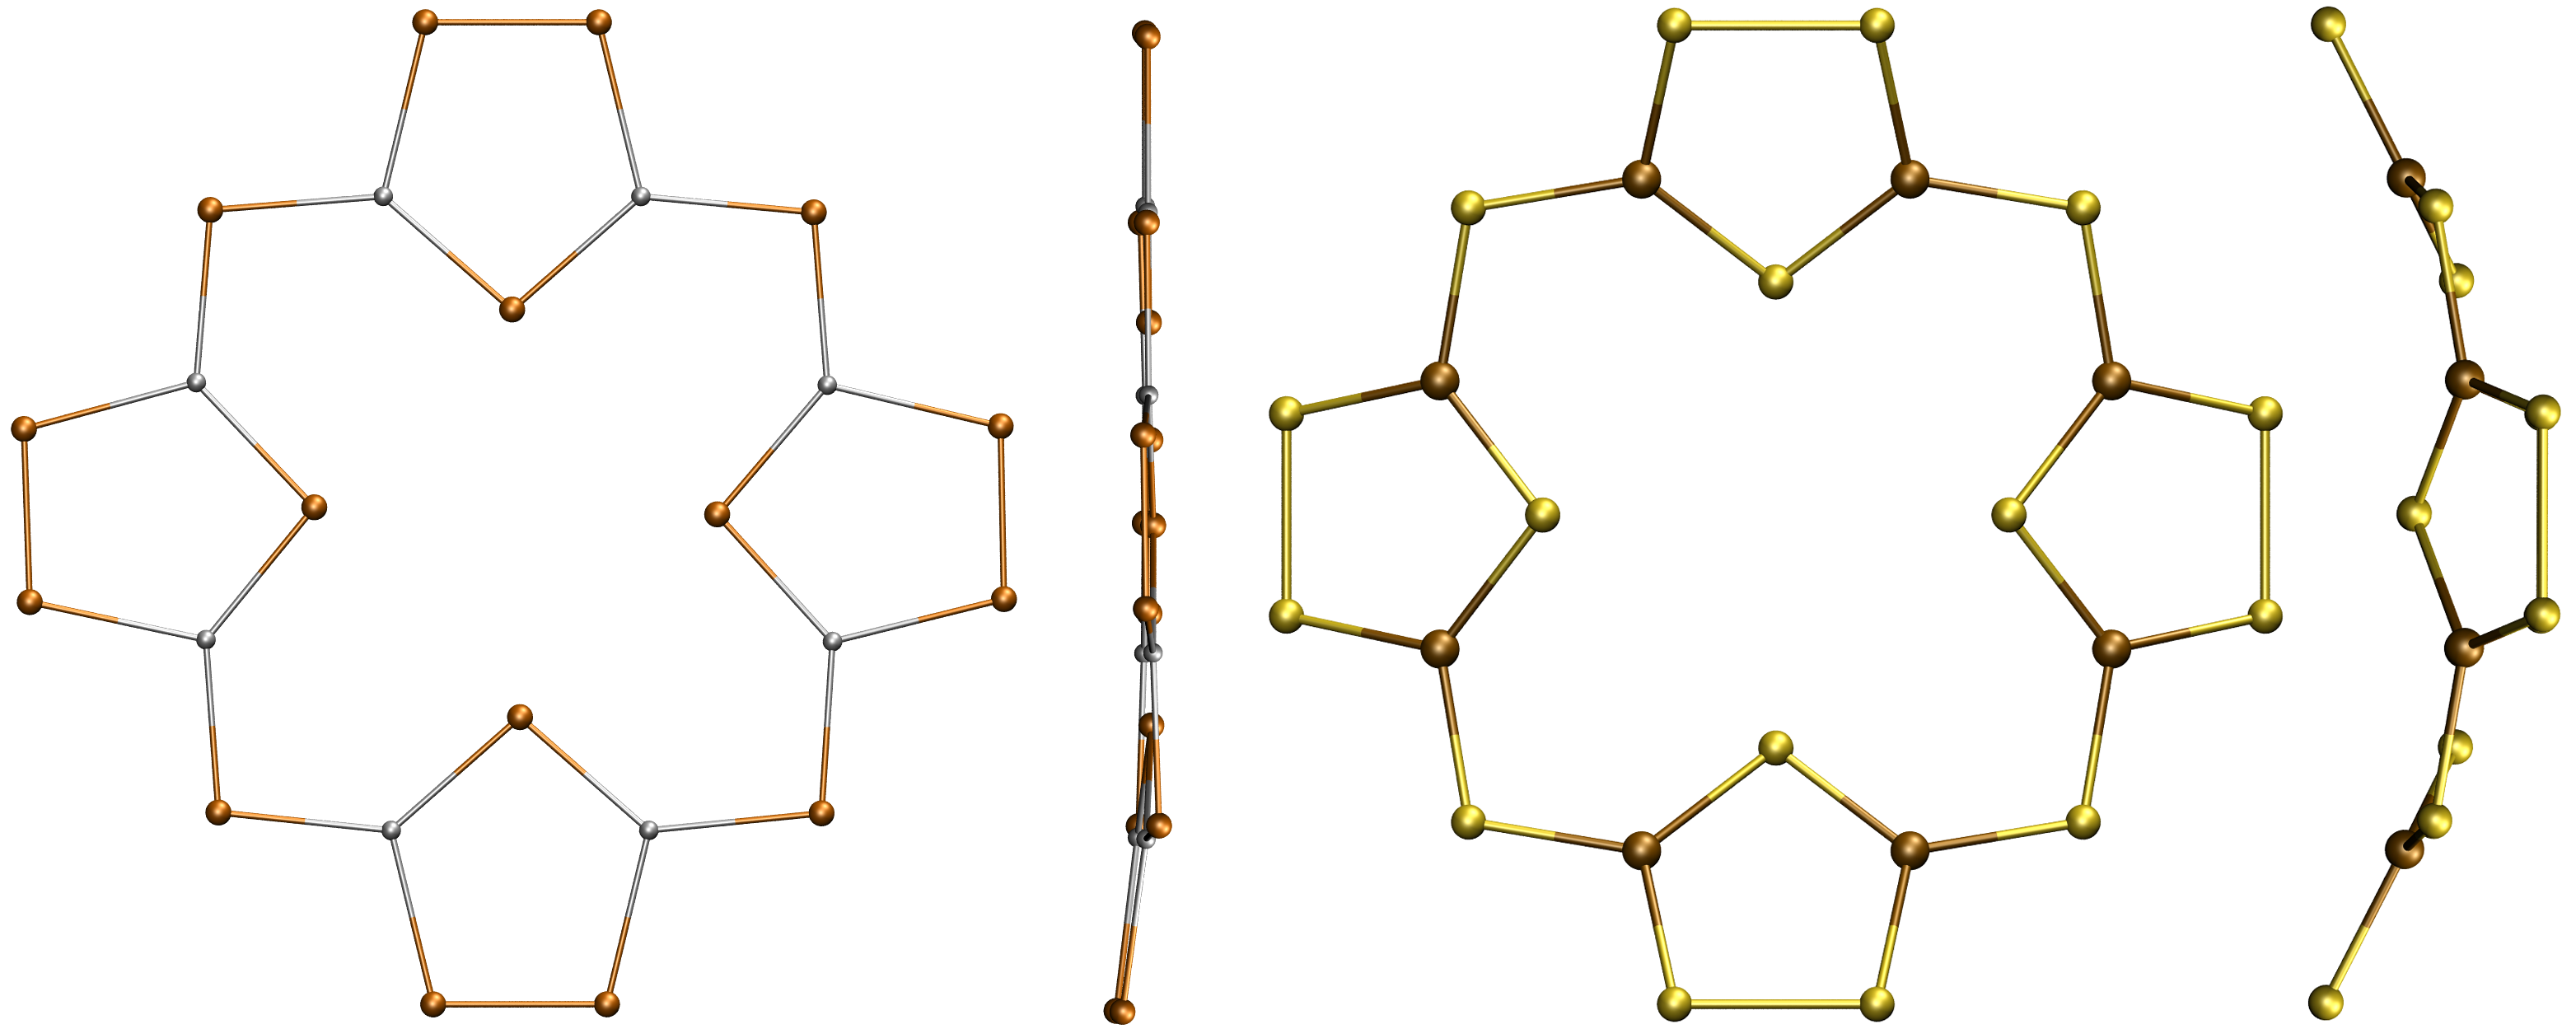
\includegraphics[width=1.0\textwidth]{hg8te16undb8s16}
	\captionsetup{figurewithin = chapter}
	\captionsetup{font=small, labelfont=bf}\caption[{Abbildung von $[$Hg$_8$Te$_{16}]^{8-}$ und B$_8$S$_{16}$}]{{Draufsicht und Seitenansicht von $[$Hg$_8$Te$_{16}]^{8-}$} (links) und B$_8$S$_{16}$ (rechts)(Quecksilber=silber, Tellur=orangebraun, Bohr=braun und Schwefel=gelb).}
\label{abb:hg8te16undb8s16}
\end{figure}
%\begin{figure}[ht!]
%	\centering
%	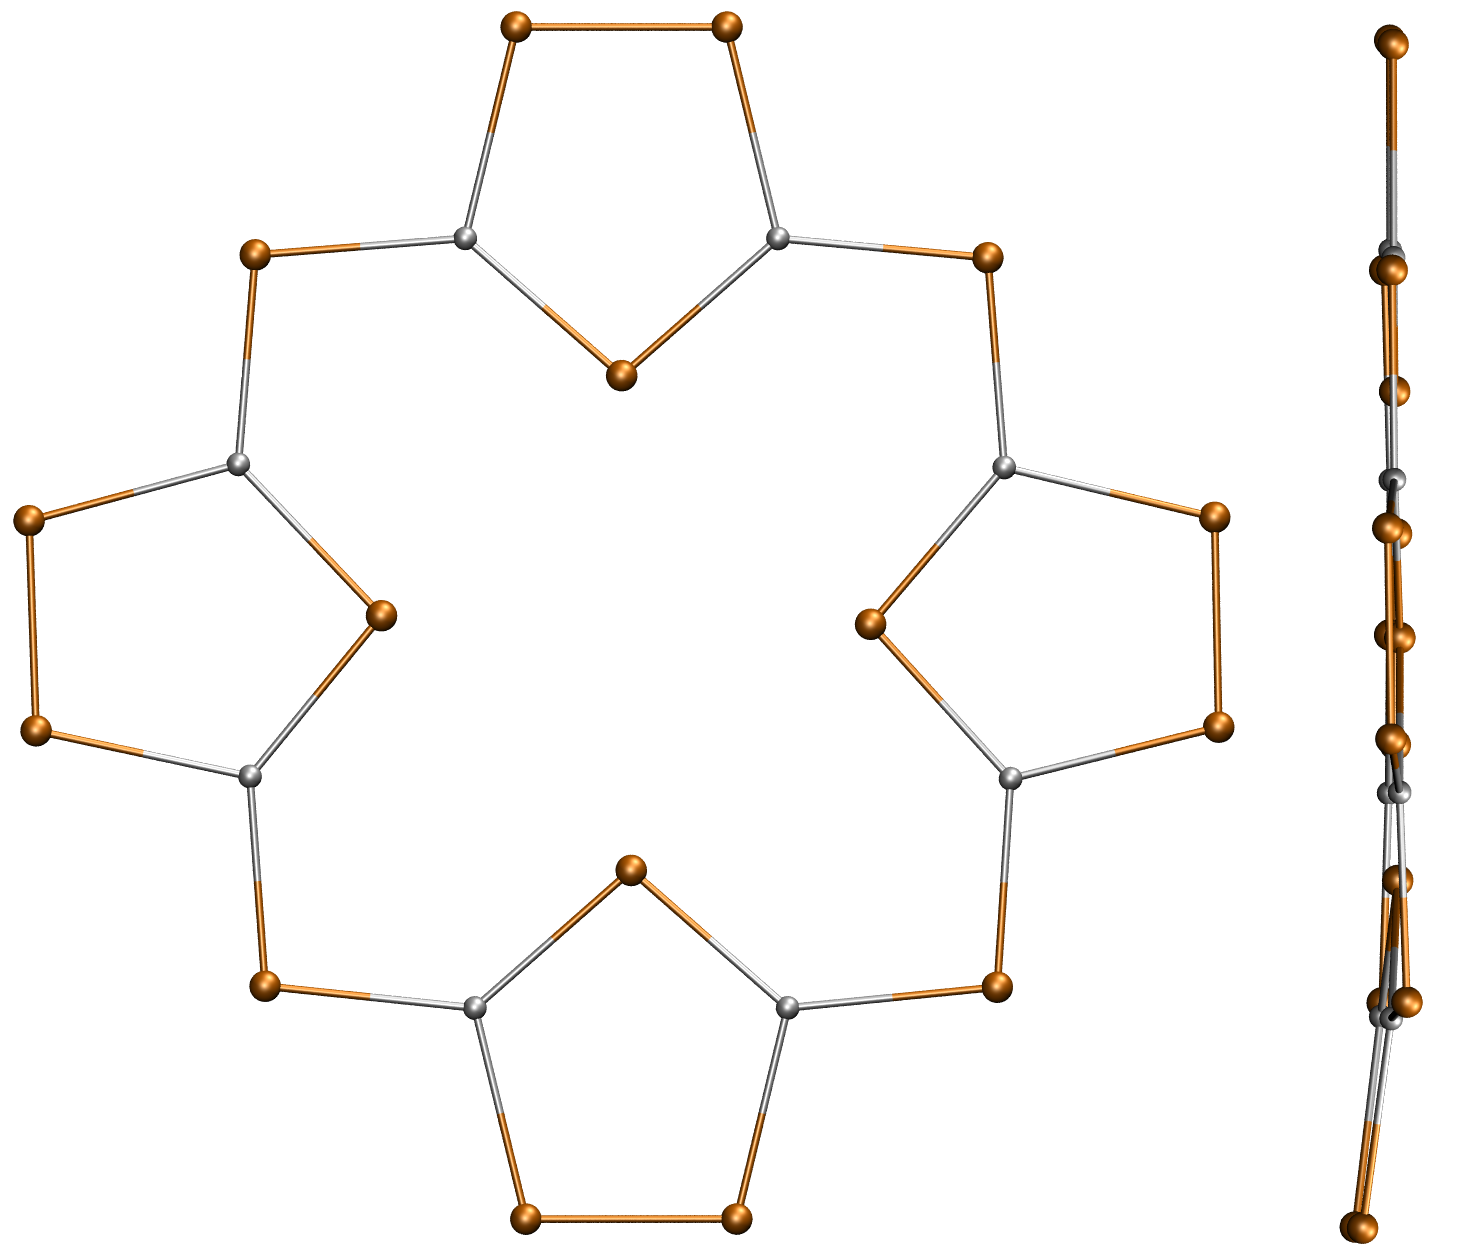
\includegraphics[width=0.6\textwidth]{hg8te16}
%	\captionsetup{figurewithin = chapter}
%	\captionsetup{font=small, labelfont=bf}\caption[{Abbildung von $[$Hg$_8$Te$_{16}]^{8-}$}]{{Abbildung von $[$Hg$_8$Te$_{16}]^{8-}$}(Quecksilber=silber, Tellur=orangebraun). Draufsicht links und Seitenansicht rechts.}
%\label{abb:hg8te16}
%\end{figure}

Zusätzlich wurde ebenfalls das bereits bekannte B$_8$S$_{16}$\supercite{krebs1980b8s16} (Abbildung \ref{abb:hg8te16undb8s16} rechts) untersucht. Hier ist die Abweichung des Moleküls mit optimierten Strukturparametern von der planaren Struktur noch deutlich größer, wie die Seitenansicht deutlich zeigt. Die $D_{4\textrm{h}}$ symmetrische Struktur weißt eine schwache imaginäre Mode von etwa -10 Wellenzahlen auf welche genau der Gerüstschwingung entspricht, welche das Durchschwingen des Moleküls beschreibt. Ebenfalls bekannt ist das schwerere Homolog B$_8$Se$_{16}$.
%\begin{figure}[ht!]
%	\centering
%	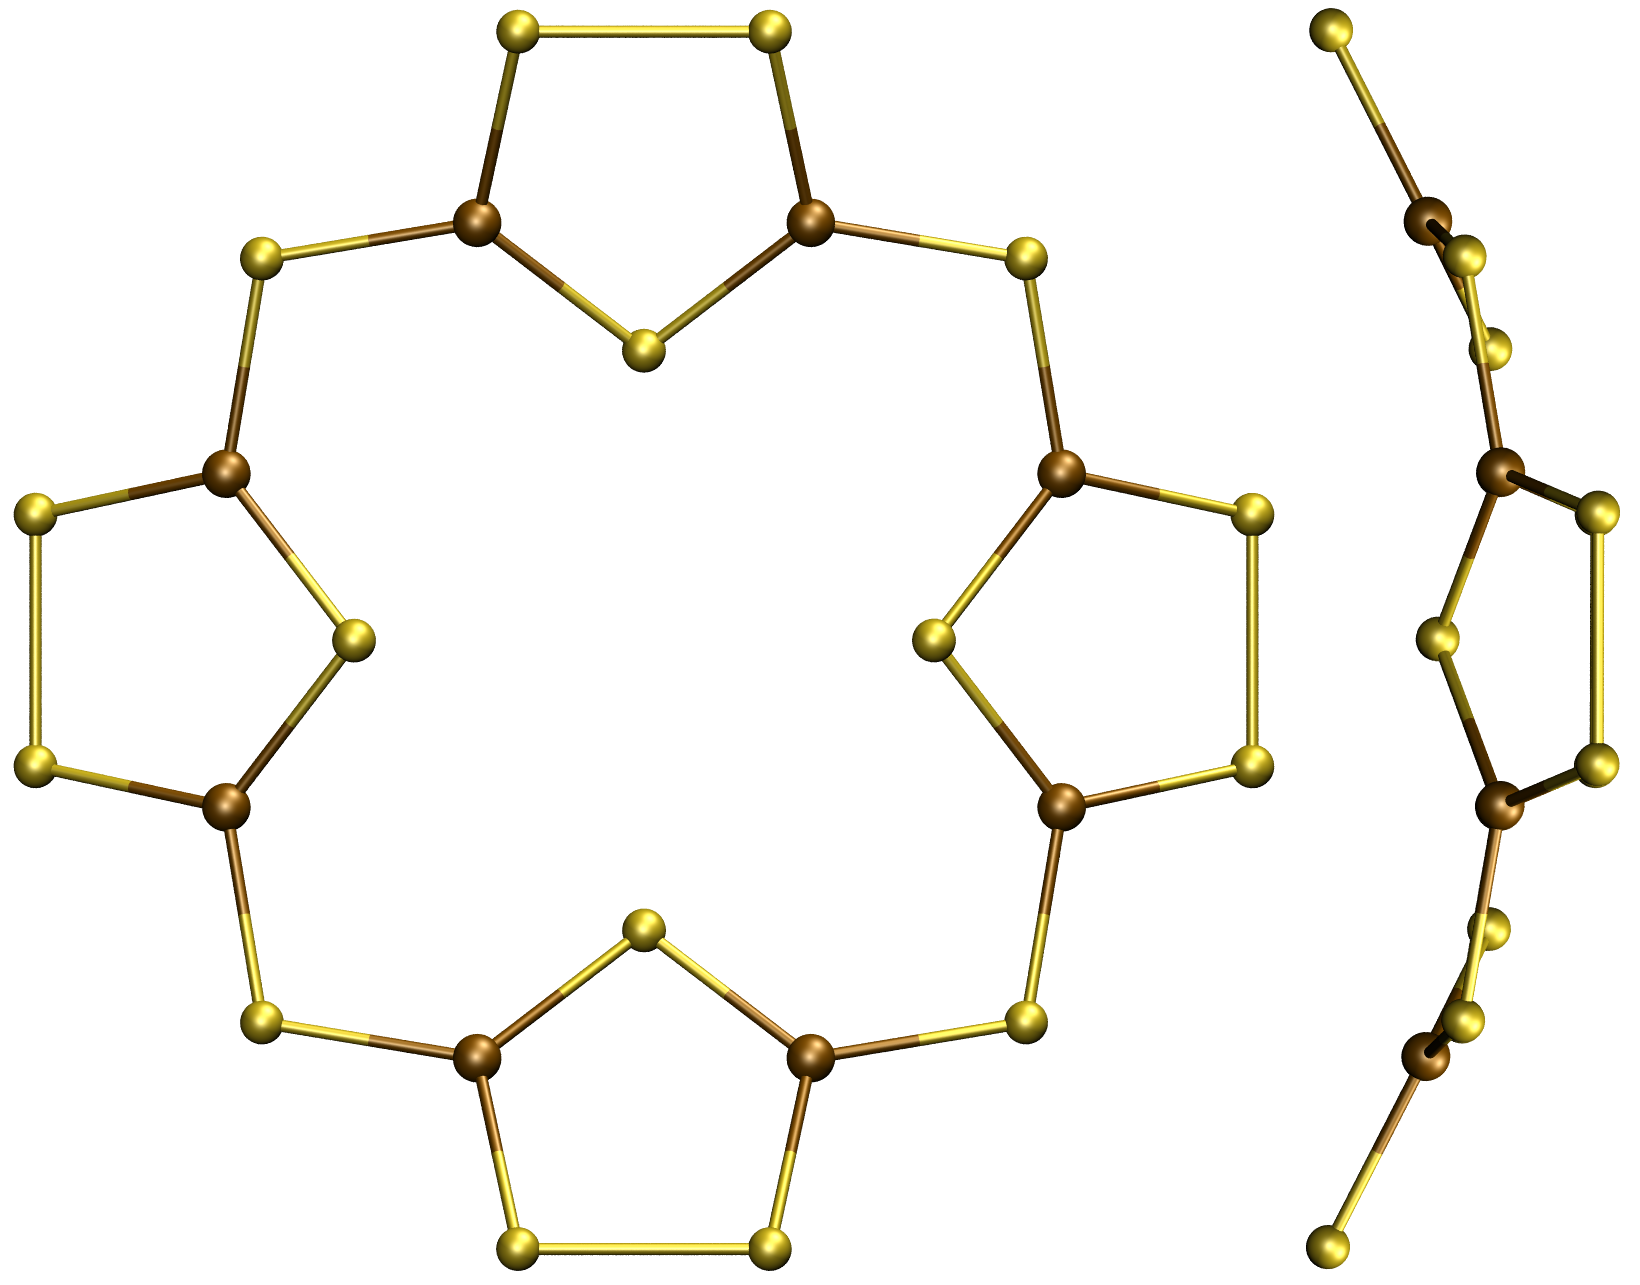
\includegraphics[width=0.6\textwidth]{b8s16}
%	\captionsetup{figurewithin = chapter}
%	\captionsetup{font=small, labelfont=bf}\caption[Abbildung von B$_8$S$_{16}$]{Abbildung von B$_8$S$_{16}$(Bohr=braun, Schwefel=gelb). Draufsicht links und Seitenansicht rechts.}
%\label{abb:b8s16}
%\end{figure}

Aufgrund ihrer strukturellen Ähnlichkeit mit dem organischen Porphyrin liegt es nahe, den aromatischen Charakter der Verbindungen zu untersuchen. Als Maß für die Aromatizität einer Verbindung kann der durch einen definierten Ring fließende Elektronenstrom - kurz Ringstrom - angesehen werden. Je diatropischer der Gesamtstrom (d.h. der Strom fließt im Uhrzeigersinn), desto aromatischer ist die Verbindung. Ein stark paratropischer Strom (Strom entgegen des Uhrzeigersinns) deutet dabei auf eine antiaromatische Verbindung hin. Sind die diatropischen und paratropischen Beiträge in etwa von der selben Größe, dann verschwindet der Gesamtstrom - die Verbindung ist nichtaromatisch. Bei der Berechnung der Ringströme mit \ac{gimic} wird dabei so vorgegangen, dass der Strom der durch eine senkrecht zur Bindungsachse stehenden Ebene fließt, integriert wird. In den oben erwähnten Beispielen kann weiterhin zwischen einem lokalen Ringstrom in den vier Fünfringen und einem globalen Ringstrom um das gesamte Molekül unterschieden werden. Bei den Berechnungen stellte sich heraus, dass alle drei Verbindungen, $[$Hg$_8$Te$_{16}]^{8-}$, B$_8$S$_{16}$ und B$_8$Se$_{16}$ einen schwachen lokalen Ringstrom in den pyrrolartigen fünfgliedrigen Ringen aufweisen. Diese betragen \unit[5.8]{nA/T} in $[$Hg$_8$Te$_{16}]^{8-}$ \unit[3.25]{nA/T} in B$_8$S$_{16}$ und \unit[3.28]{nA/T} in B$_8$Se$_{16}$. Im Vergleich dazu beträgt der Ringstrom in einem Benzolmolekül etwa \unit[12]{nA/T}\supercite{fliegl2012aromatic}. Die globalen Ringströme in den drei Verbindungen sind mit \unit[0.24]{nA/T}, \unit[0.81]{nA/T} und \unit[0.79]{nA/T} verschwindend gering. Im Vergleich dazu liegt der globale Ringstrom des organischen Porphyrins bei etwa \unit[27]{nA/T}. Dieser spaltet sich in den fünfgliedrigen Ringen in einen äußeren und inneren Pfad auf, welche jeweils einen Ringstrom von etwa \unit[13]{nA/T} aufweisen. Der lokale Ringstrom in den fünfgliedrigen Ringen ist schwächer als \unit[1]{nA/T}.\supercite{fliegl2012aromatic} In sogenannten \ac{lic} Plots lassen sich die Ringströme in einer gewählten Ebene visualisieren. Dies wurde für das organische Porphyrin und die drei Verbindungen $[$Hg$_8$Te$_{16}]^{8-}$, B$_8$S$_{16}$ und B$_8$Se$_{16}$ gemacht und die entsprechenden Plots sind in der Abbildung \ref{abb:lic} zu sehen. Beim Porphyrin ist eindeutig der globale Ringstrom zu erkennen, welcher sich in den fünfgliedrigen Ringen in zwei Pfade aufspaltet. im Vergleich dazu weisen die anderen Verbindungen lediglich schwache lokale Ströme in den fünfgliedrigen Ringen auf.
Diese Befunde lassen sich dadurch erklären, dass im Porphyrin eine völlig andere elektronische Situation vorliegt. Die Aromatizität und die damit verbundenen Ringströme basieren auf einem delokalisierten $\pi$-System. Beispielsweise lassen sich im $[$Hg$_8$Te$_{16}]^{8-}$ alle \acp{mo} durch Anwenden einer Lokalisierungsprozedur\supercite{boys1960sf} zu Zweizentren-Zweielektronen-Bindungen und freien Elektronenpaaren lokalisieren. Dabei werden s-artige Einfachbindungen zwischen den benachbarten Atomen und zwei freie Elektronenpaare pro Telluratom erhalten. 

 

\begin{figure}[ht!]
	\centering
	\includegraphics[width=1.0\textwidth]{1bohr}
	\captionsetup{figurewithin = chapter}
	\captionsetup{font=small, labelfont=bf}\caption[{Ringströme in Porphyrin, $[$Hg$_8$Te$_{16}]^{8-}$, B$_8$S$_{16}$ und B$_8$Se$_{16}$}]{Ringströme in Porphyrin (oben links), $[$Hg$_8$Te$_{16}]^{8-}$ (oben rechts), B$_8$S$_{16}$ (unten links) und B$_8$Se$_{16}$ (unten rechts) \unit[1]{bohr} oberhalb der Molekülebene, dargestellt zwischen \unit[0]{a.u.} (blau) und \unit[0.07]{a.u.}.}
\label{abb:lic}
\end{figure}

\FloatBarrier
Das fehlende $\pi$-System im $[$Hg$_8$Te$_{16}]^{8-}$ sorgt für eine gewisse strukturelle Flexibilität des Makrozyklus. Dadurch können unterschiedliche Koordinationspolyeder und Koordinationszahlen realisiert werden. Die Strukturparameter wurden exemplarisch für der Komplexierung der Metallkationen Zn$^{2+}$, Cu$^+$ , Ce$^{4+}$ und Ti$^{4+}$ optimiert und die erhaltenen Strukturen sind in Abbildung \ref{abb:komplexierung} gezeigt. Für Zn$^{2+}$ und Cu$^+$ ist zu erkennen, dass es dabei im Wesentlichen zu einer Verzerrung des Makrozyklus kommt um eine tetraedrische Koordination zu ermöglichen. Im Falle der Ce$^{4+}$ und Ti$^{4+}$ Kationen führt die Komplexierung zu einer deutlich ausgeprägteren Umordnung der Atome. Damit lässt sich sowohl die bevorzugt größere Koordinationszahl des Ce$^{4+}$ als auch die Anpassung an den deutlich geringeren Ionenradius des Ti$^{4+}$ realisieren.

\begin{figure}[ht!]
	\centering
	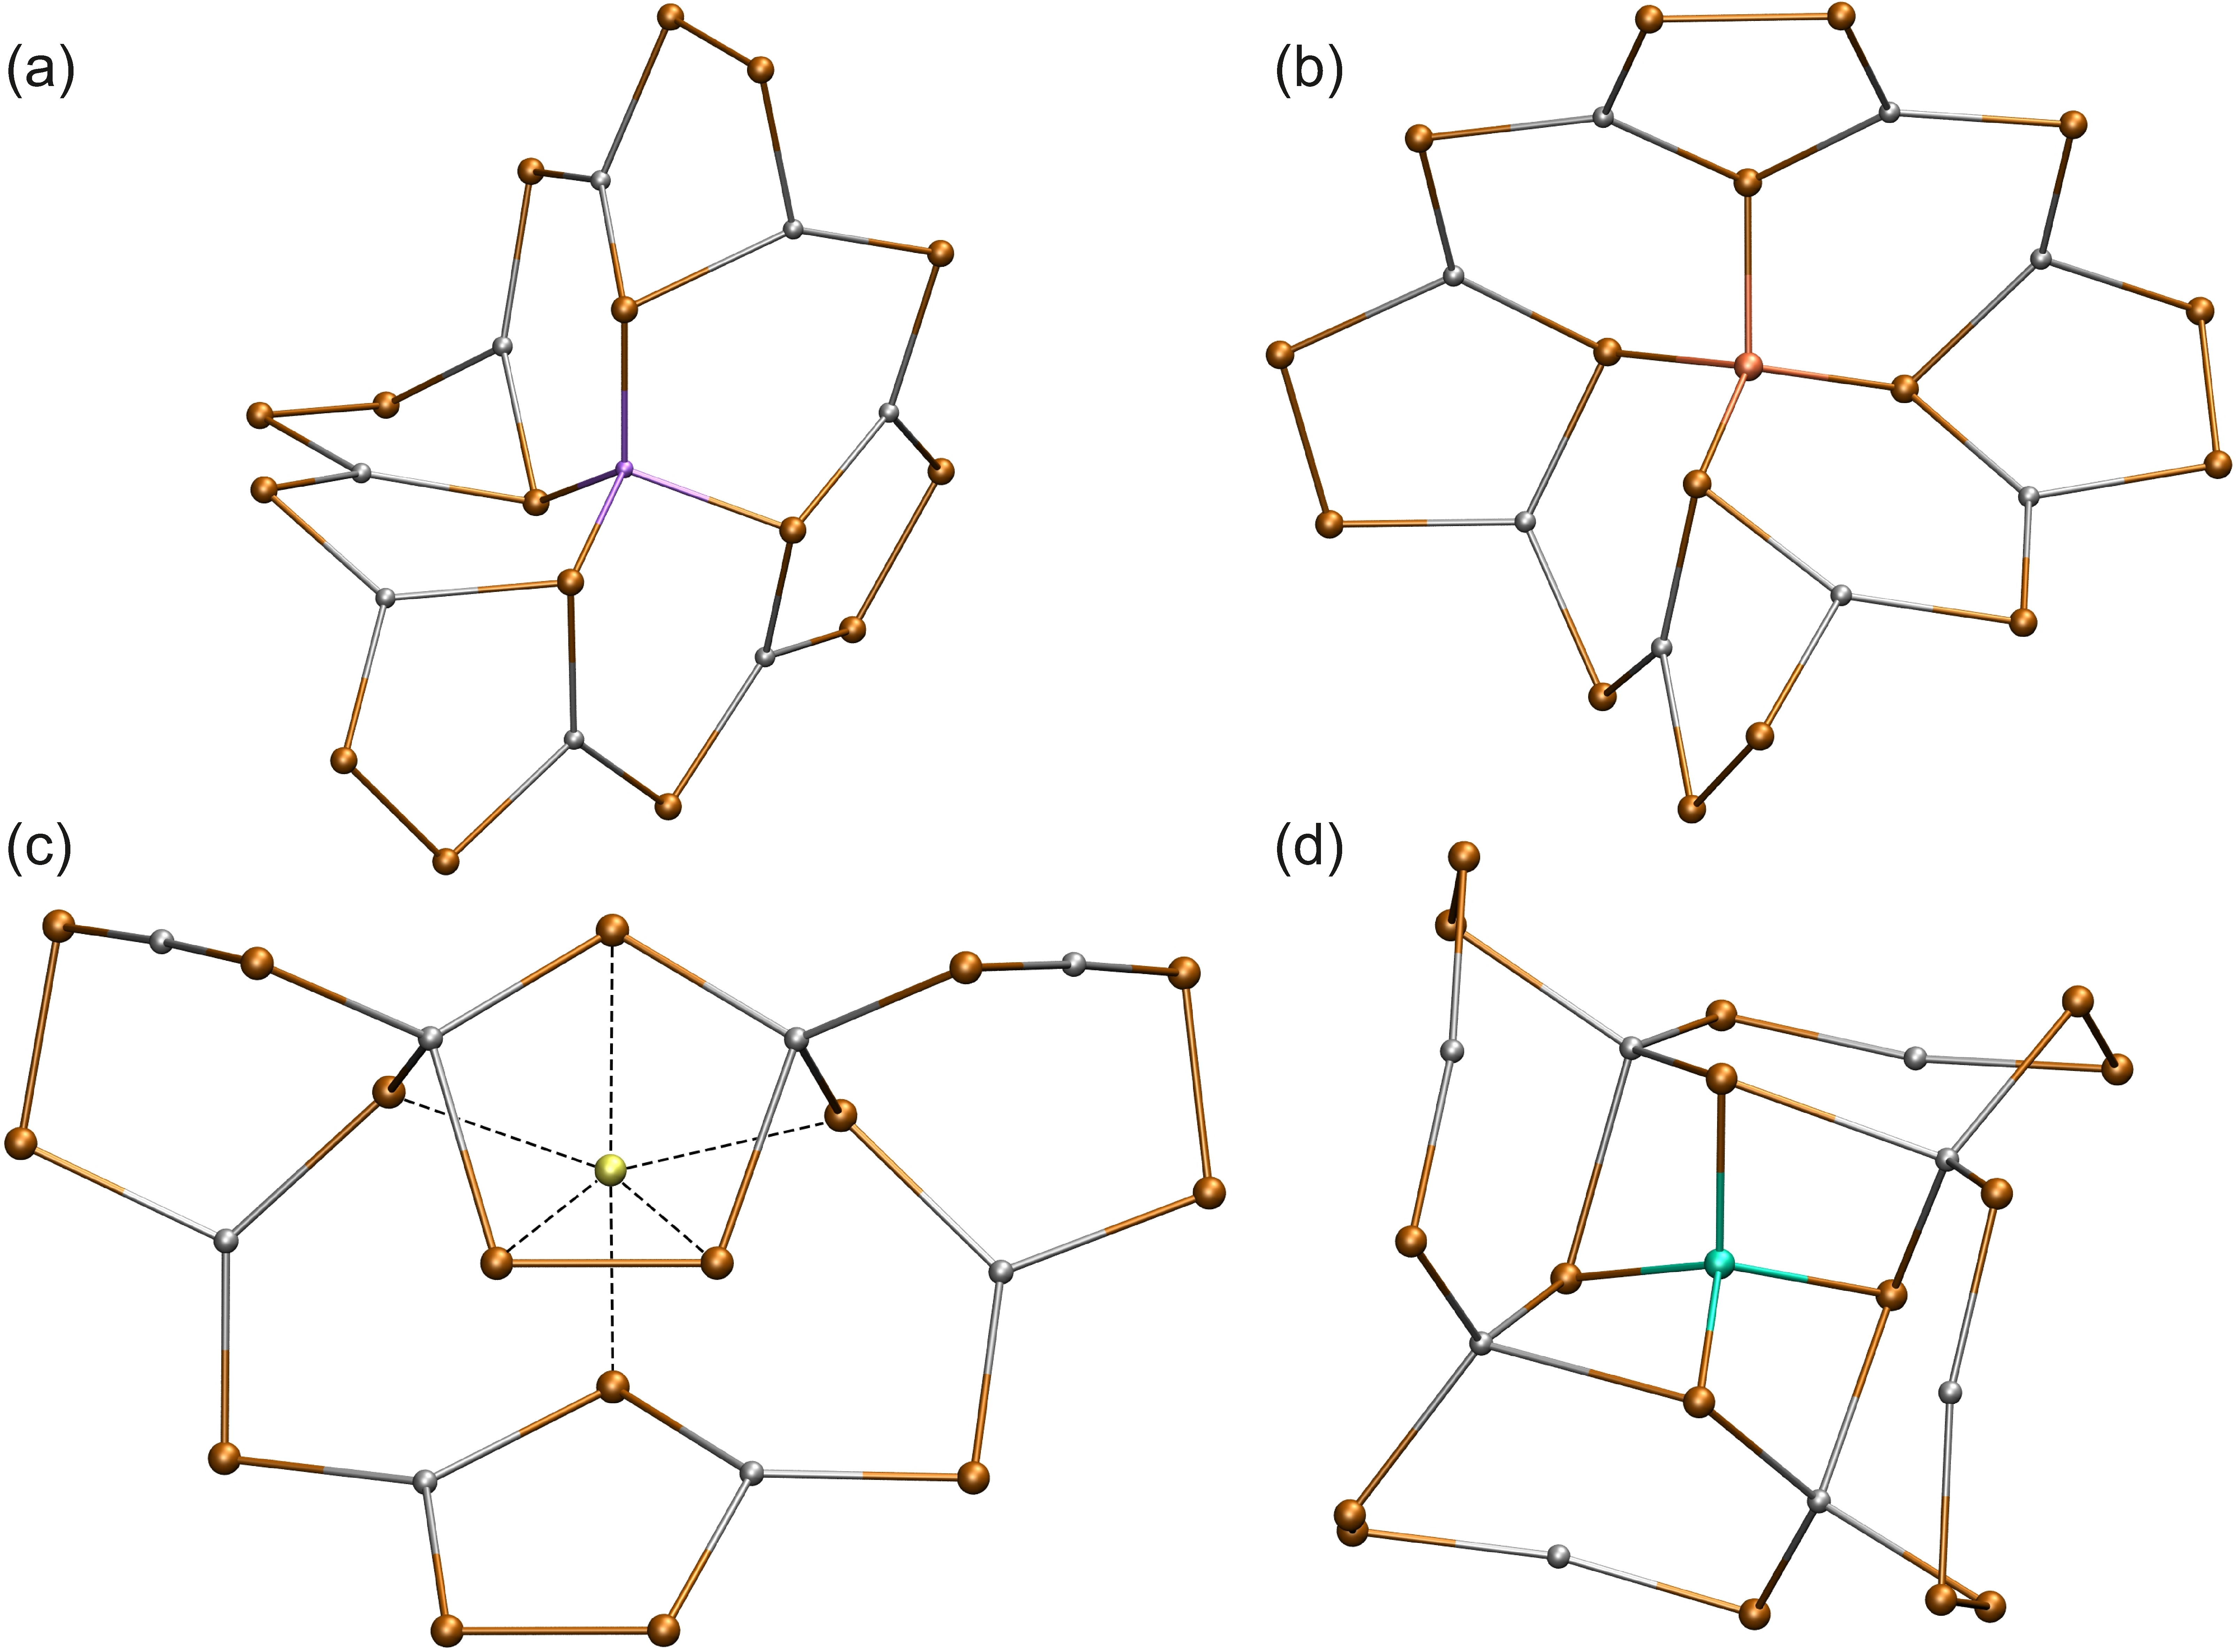
\includegraphics[width=1.0\textwidth]{komplexierung}
	\captionsetup{figurewithin = chapter}
	\captionsetup{font=small, labelfont=bf}\caption[{Abbildungen der hypothetischen Komplexe [M@Hg$_8$Te$_{16}]^{(8-q)-}$ (M$^{q+}$ = Zn$^{2+}$, Cu$^+$ , Ce$^{4+}$ und Ti$^{4+}$)}]{{Abbildung der hypothetischen Komplexe [M@Hg$_8$Te$_{16}]^{(8-q)-}$ (M$^{q+}$ = Zn$^{2+}$ (oben links), Cu$^+$ (oben rechts), Ce$^{4+}$ (unten links) und Ti$^{4+}$ (unten rechts))} zur Veranschaulichung der strukturellen Flexibilität von $[$Hg$_8$Te$_{16}]^{8-}$ (Quecksilber=silber, Tellur=orangebraun, Zink=lilablau, Kupfer=kupfer, Cer=hellgelb, Titan=türkis). }
\label{abb:komplexierung}
\end{figure}

%\begin{figure}[ht!]
%	\centering
%	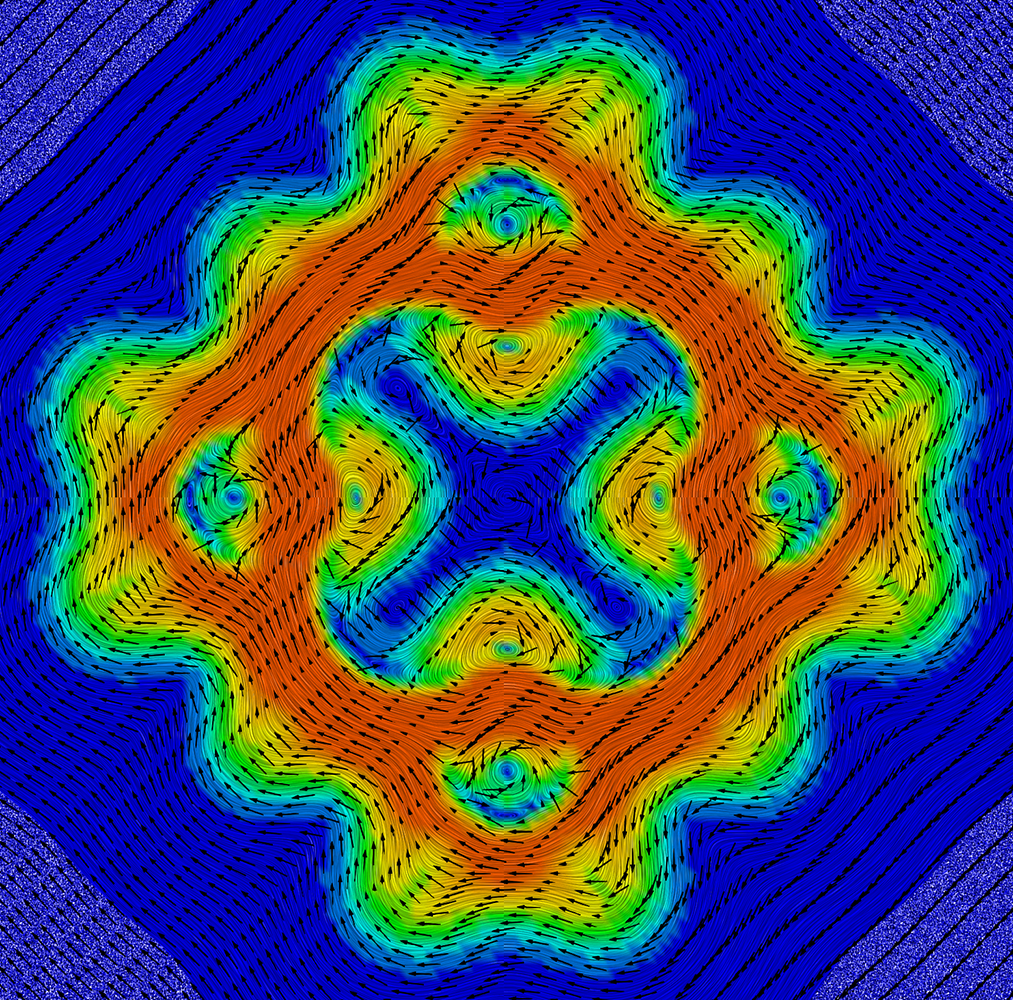
\includegraphics[width=0.6\textwidth]{porph_1bohr}
%	\captionsetup{figurewithin = chapter}
%	\captionsetup{font=small, labelfont=bf}\caption[Ringströme in Porphyrin]{Ringströme in Porphyrin \unit[1]{bohr} oberhalb der Molekülebene, dargestellt zwischen \unit[0]{a.u.} (blau) und \unit[0.07]{a.u.}.}
%\label{abb:porphlic}
%\end{figure}
%
%\begin{figure}[ht!]
%	\centering
%	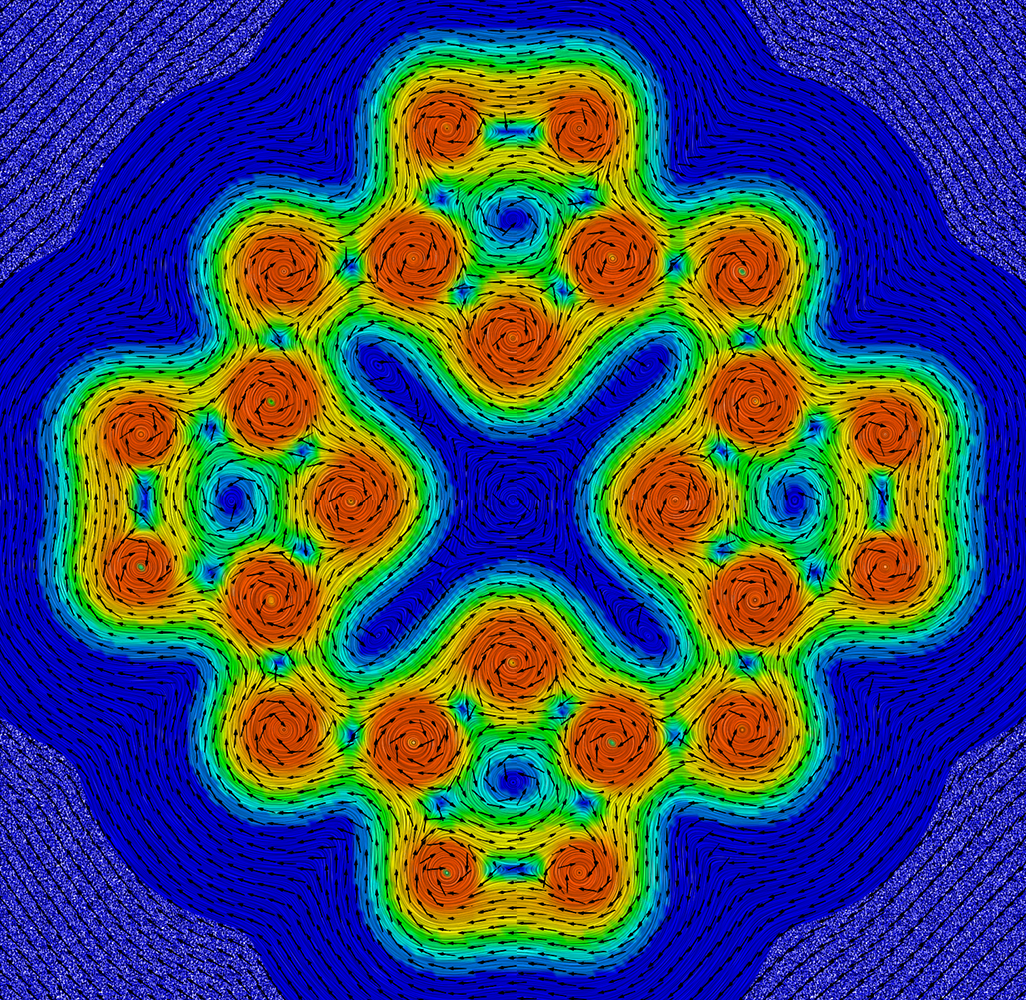
\includegraphics[width=0.6\textwidth]{hgte_1bohr}
%	\captionsetup{figurewithin = chapter}
%	\captionsetup{font=small, labelfont=bf}\caption[{Ringströme in $[$Hg$_8$Te$_8$(Te$_2$)$_4]^{8-}$}]{Ringströme in $[$Hg$_8$Te$_8$(Te$_2$)$_4]^{8-}$ \unit[1]{bohr} oberhalb der Molekülebene, dargestellt zwischen \unit[0]{a.u.} (blau) und \unit[0.07]{a.u.}.}
%\label{abb:hgtelic}
%\end{figure}
%
%\begin{figure}[ht!]
%	\centering
%	\includegraphics[width=0.6\textwidth]{b8s16_1bohr}
%	\captionsetup{figurewithin = chapter}
%	\captionsetup{font=small, labelfont=bf}\caption[Ringströme in B$_8$S$_{16}$]{Ringströme in B$_8$S$_{16}$ \unit[1]{bohr} oberhalb der Molekülebene, dargestellt zwischen \unit[0]{a.u.} (blau) und \unit[0.07]{a.u.}.}
%\label{abb:b8s16hlic}
%\end{figure}
%
%\begin{figure}[ht!]
%	\centering
%	\includegraphics[width=0.6\textwidth]{b8se16_1bohr}
%	\captionsetup{figurewithin = chapter}
%	\captionsetup{font=small, labelfont=bf}\caption[Ringströme in B$_8$Se$_{16}$]{Ringströme in B$_8$Se$_{16}$ \unit[1]{bohr} oberhalb der Molekülebene, dargestellt zwischen \unit[0]{a.u.} (blau) und \unit[0.07]{a.u.}.}
%\label{abb:b8se16hlic}
%\end{figure}

\FloatBarrier
\subsection{\texorpdfstring{[Co@Sn$_6$Sb$_6$]$^{3-}$ und [Co$_2$@Sn$_5$Sb$_7$]$^{3-}$}{[Co at Sn\_6Sb\_6]3- und [Co\_2 at Sn\_5Sb\_7]3-}}
Wie bereits in der Einleitung dieser Arbeit erwähnt wurde, kann die Zuordnung einzelner Signale in experimentell gemessenen \ac{nmr} Spektren in machen Fällen eine große Herausforderung darstellen. Zwei exemplarische Beispiele dafür sind die $^{119}$Sn \ac{nmr} Spektren der in der Arbeitsgruppe von Stefanie Dehnen synthetisierten Clustersanionen [Co@Sn$_6$Sb$_6$]$^{3-}$ und [Co$_2$@Sn$_5$Sb$_7$]$^{3-}$.\supercite{wilson2018structure} Die grundlegende Struktur dieser endohedralen Komplexe besteht aus zwei verbundenen quadratischen Antiprismen und ist in Abbildung \ref{abb:coatsnsb} dargestellt. Interessanterweise befindet sich das Cobaltatom im Falle des [Co@Sn$_6$Sb$_6$]$^{3-}$ nicht im Zentrum des gesamten Clusteranions, sondern im Zentrum eines der quadratischen Antiprismen. Mit Hilfe des genetischen Algorithmus\supercite{weigend2014extending} konnten diese ungewöhnlichen Strukturen auf \ac{dft}-Niveau bestätigt werden. Die Zuordnung der Atomsorten erfolgt darin über einen störungstheoretischen Ansatz. Für den genetischen Algorithmus wurde das BP86 Funktional\supercite{perdew1986density,becke1988density} und der def-SV(P) Basissatz\supercite{eichkorn1997auxiliary} verwendet. Die Anzahl der Generationen wurde auf 30 und die Anzahl der Strukturen je Generationen auf 25 festgelegt. In jeder Generation wurden die 13 energetisch ungünstigsten Strukturen durch neu generierte ersetzt. Alle 25 Strukturen der letzten Generation weisen das Grundgerüst von zwei verknüpften quadratischen Antiprismen auf, welches für die energetisch höher liegenden Isomere jedoch stärker verzerrt ist. Die Strukturparameter der Strukturen aus der letzten Generation wurden  mit dem TPSS Funktional\supercite{tao2003climbing} und der dhf-TZVP Basis\supercite{weigend2010segmented} sowie den zugehörigen \acp{ecp}\supercite{metz2000small} für Zinn und Antimon nach optimiert. Die negative Ladung wurde mit Hilfe des \acp{cosmo}\supercite{klamt1993cosmo} unter Verwendung der Standardeinstellungen kompensiert. Insgesamt unterscheiden sich die Strukturen im Wesentlichen durch die Verteilung der Atomsorten und liegen in einem Energiebereich von \unit[37]{kJ/mol} ([Co@Sn$_6$Sb$_6$]$^{3-}$) und \unit[22]{kJ/mol} ([Co$_2$@Sn$_5$Sb$_7$]$^{3-}$). Für die erste Verbindung wurden zwei nahezu isoenergetische Isomere gefunden (linke Seite und Mitte von Abbildung \ref{abb:coatsnsb}). Die energetisch günstigste Struktur des zweiten Clusteranions ist auf der rechten Seite der Abbildung gezeigt.

\begin{figure}[ht!]
	\centering
	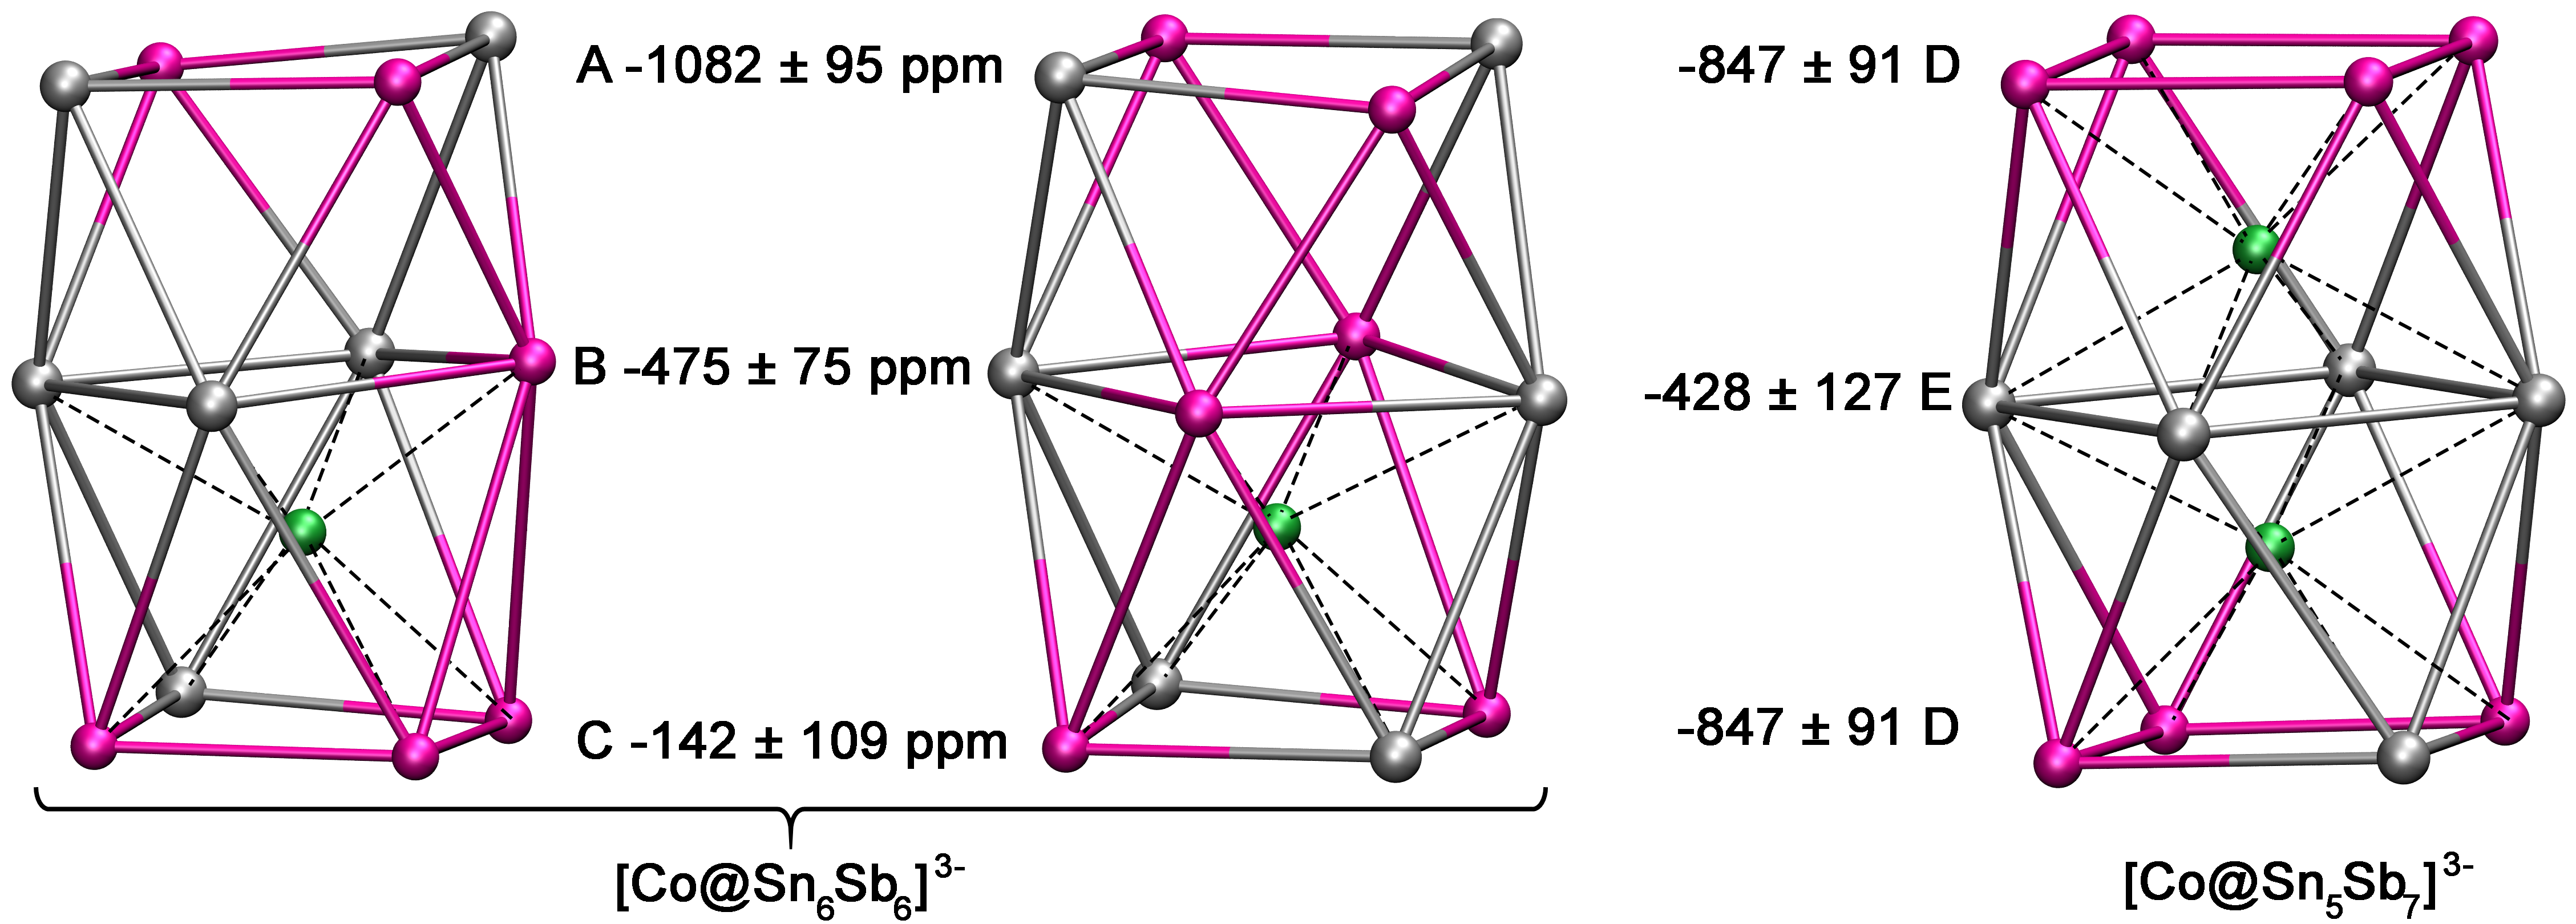
\includegraphics[width=1.0\textwidth]{coatsnsb}
	\captionsetup{figurewithin = chapter}
	\captionsetup{font=small, labelfont=bf}\caption[Strukturen von {[Co@Sn$_6$Sb$_6$]$^{3-}$ und [Co$_2$@Sn$_5$Sb$_7$]$^{3-}$}]{Strukturen der energetisch am tiefsten liegenden Isomere von [Co@Sn$_6$Sb$_6$]$^{3-}$ (links und Mitte) und [Co$_2$@Sn$_5$Sb$_7$]$^{3-}$ (rechts). Zusätzlich sind die gemittelten $^{119}$Sn chemischen Verschiebungen sowie die zugehörigen Standardabweichungen für die viergliedrigen Ringe A-E in ppm angegeben. Dabei wurden alle Isomere in einem Energiebereich von \unit[10]{kJ/mol} relativ zum energetisch günstigsten Isomer (siehe auch Tabelle \ref{tab:snnmrtab1} bis Tabelle \ref{tab:snnmrtab3}) einbezogen. (Zinn=hellgrau, Antimon=magenta, Cobalt=grün).}
\label{abb:coatsnsb}
\end{figure}
\FloatBarrier
Aufgrund der vergleichsweise langen Zeitskala bei \ac{nmr} Experimenten kann die Zuordnung der gemessenen Peaks auf die einzelnen Positionen durch intramolekularen Austausch zusätzlich erschwert werden. Das experimentelle $^{119}$Sn \ac{nmr} Spektrum des in DMF-d$_7$ gelösten Einkristalls [K(crypt-222)]$_3$\{[Co@Sn$_6$Sb$_6$]$^{3-}$\}$_{0.83}$\{[Co$_2$@Sn$_5$Sb$_7$]$^{3-}$\}$_{0.17}\cdot$2dmf$\cdot$2tol ist oben und das Spektrum von [K(crypt-222)]$_3$[Co$_2$@Sn$_5$Sb$_7$]$^{3-}$ ist unten in Abbildung \ref{abb:expsnnmr} gezeigt. Beide Spektren weisen mehrere scharfe Linien auf, wodurch hier von einem wenig dynamischen Verhalten in Lösung ausgegangen werden kann. Das obere Spektrum, welches beide Verbindungen beinhaltet, besitzt in den Bereichen D und E Singnale, welche im Spektrum des reinen [K(crypt-222)]$_3$[Co$_2$@Sn$_5$Sb$_7$]$^{3-}$ deutlich an Intensität gewinnen und sich somit dieser Verbindung zuordnen lassen. Zusätzlich verschwinden dort die Signale aus den Bereichen A-C, wodurch diese Peaks der anderen Struktur zugeordnet werden können. 
\begin{figure}[ht!]
	\centering
	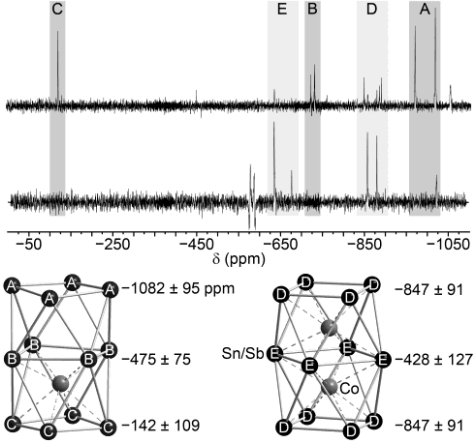
\includegraphics[width=1.0\textwidth]{snnmrspectra}
	\captionsetup{figurewithin = chapter}
	\captionsetup{font=small, labelfont=bf}\caption[{$^{119}$Sn \ac{nmr} Spektren von [Co@Sn$_6$Sb$_6$]$^{3-}$ und [Co$_2$@Sn$_5$Sb$_7$]$^{3-}$}]{Experimentelle $^{119}$Sn \ac{nmr} Spektren von [K(crypt-222)]$_3$\{[Co@Sn$_6$Sb$_6$]$^{3-}$\}$_{0.83}$\{[Co$_2$@Sn$_5$Sb$_7$]$^{3-}$\}$_{0.17}\cdot$2dmf$\cdot$2tol (oben) und [K(crypt-222)]$_3$[Co$_2$@Sn$_5$Sb$_7$]$^{3-}$ (unten) in DMF-d$_7$.}
\label{abb:expsnnmr}
\end{figure}
\FloatBarrier

Für die Zuordnung der Peaks auf die atomaren Positionen wurden die Sn Verschiebungen für die Isomere beider Clusteranionen mit einer relativen Energie von bis zu \unit[10]{kJ/mol} berechnet (siehe Tabelle \ref{tab:snnmrtab1} und \ref{tab:snnmrtab2}). Die Berechnungen wurden mit den selben Einstellungen wie bei der Optimierung der Strukturparameter durchgeführt, mit der Ausnahme, dass für Zinn die TZVPPall Basis\supercite{ahlrichs2000contracted} verwendet wurde. Zur Vereinfachung wurden die chemischen Verschiebungen in den jeweiligen viergliedrigen Ringen A-E (siehe Abbildung \ref{abb:coatsnsb}) gemittelt. Da die einzelnen chemischen Verschiebungen sowohl innerhalb eines dieser Ringe in einem Isomer als auch zwischen den einzelnen Isomeren variieren kann, können mehrere Signale aus dem Spektrum einem Ring zugehörig sein. Wie deutlich zu erkennen ist, wird durch die \ac{dft}-Rechnung eine deutliche Aufspaltung zwischen den äußeren Ringen A (\unit[-1082 $\pm$ 95]{ppm}) und C (\unit[-142 $\pm$ 109]{ppm}) erhalten. Der am höchsten gelegene Peak bei \unit[-119]{ppm} korreliert daher am besten mit Ring C, die beiden Peaks bei \unit[-970]{ppm} und \unit[-1018]{ppm} mit Ring A. Der verbleibende Peak bei \unit[-731]{ppm} kann folglich dem zentralen Ring B zugeordnet werden. Aus der Berechnung der chemischen Verschiebungen für [Co$_2$@Sn$_5$Sb$_7$]$^{3-}$ ergibt sich eine stärkere Abschirmung der Zinnatome in den äußeren Ringen D (\unit[-847 $\pm$ 91]{ppm}) als für die Zinnatome im zentralen Ring E (\unit[-428 $\pm$ 127]{ppm}). Dadurch erfolgt die Zuordnung der Peaks bei \unit[-634]{ppm} und \unit[-676]{ppm} zu Ring E und die der Peaks zwischen \unit[-849]{ppm} und \unit[-890]{ppm} zu den äußeren Ringen D. 

\begin{table}[ht!]
\captionsetup{tablewithin = chapter}
\captionsetup{font=small, labelfont=bf}
\captionabove[{$^{119}$Sn chemische Verschiebungen von [Co@Sn$_6$Sb$_6$]$^{3-}$}]{Relative Energien $E$ und $^{119}$Sn chemische Verschiebungen in Bezug auf SnMe$_4$ in ppm für die 10 stabilsten Isomere \textbf{A}-\textbf{J} von [Co@Sn$_6$Sb$_6$]$^{3-}$. Alle Berechnungen wurden mit TPSS/COSMO (mit Standardeinstellungen), der dhf-TZVP Basis für Co und Sb und der all-Elektronen Basis TZVPPall für Sn durchgeführt.}
\resizebox{\textwidth}{!}{%
\begin{tabular}{cccccccccccccc}
\hline \hline
  & $E$ & \textbf{1} & \textbf{2} & \textbf{3} & \textbf{4} & \textbf{5} & \textbf{6} & \textbf{7} & \textbf{8} & \textbf{9} & \textbf{10} & \textbf{11} & \textbf{12} \\
  & kJ/mol  & & & & & & & & & & & &\\
  \hline
  \textbf{A} & 0 & & -1089 & & -1088 & & -538 & -522 & -404 & & & -335 &\\
  \textbf{B} & 2.6 & & -1122 & & -1125 & -542 & & -539 & & -137 & & -132 &\\
  \textbf{C} & 3.2 & & -1087 & -1153 & & -337 & -578 & & -462 & & & -117 &\\
  \textbf{D} & 3.9 & -1194 & & -960 & & -413 & -453 & -463 & & & & -147 &\\
  \textbf{E} & 4.2 & -1185 & & -943 & & & -436 & -466 & -426 & & & -165 &\\
  \textbf{F} & 8.1 & -1131 & & -904 & & -447 & -567 & & -349 & & & 40 &\\
  \textbf{G} & 11.2 & -1046 & & -1044 & & & -517 & & -519 & 99 & & 105 &\\
  \textbf{H} & 14.1 & & -1020 & & -1289 & -456 & -456 & & & -184 & & -184 &\\
  \textbf{I} & 16.6 & & & -1229 & -1476 & -241 & -591 & & -523 & & & 148 &\\
  \textbf{J} & 17.4 & -996 & & -999 & & -407 & -404 & & & 23 & & 35 &\\
\end{tabular}}
\label{tab:snnmrtab1}
\end{table}

\begin{table}[ht!]
\captionsetup{tablewithin = chapter}
\captionsetup{font=small, labelfont=bf}
\captionabove[{$^{119}$Sn chemische Verschiebungen von [Co$_2$@Sn$_5$Sb$_7$]$^{3-}$}]{Relative Energien $E$ und $^{119}$Sn chemische Verschiebungen in Bezug auf SnMe$_4$ in ppm für die 15 stabilsten Isomere \textbf{A}-\textbf{O} von [Co$_2$@Sn$_5$Sb$_7$]$^{3-}$. Alle Berechnungen wurden mit TPSS/COSMO (mit Standardeinstellungen), der dhf-TZVP Basis für Co und Sb und der all-Elektronen Basis TZVPPall für Sn durchgeführt.}
\resizebox{\textwidth}{!}{%
\begin{tabular}{cccccccccccccc}
\hline \hline
  & $E$ & \textbf{1} & \textbf{2} & \textbf{3} & \textbf{4} & \textbf{5} & \textbf{6} & \textbf{7} & \textbf{8} & \textbf{9} & \textbf{10} & \textbf{11} & \textbf{12} \\
  & kJ/mol  & & & & & & & & & & & &\\
  \hline
  \textbf{A} & 0 & & & & & -387 & -527 & -523 & -383 & & & -993 &\\
  \textbf{B} & 3.7 & & & -715 & & -238 & -628 & & -302 & & & -715 &\\
  \textbf{C} & 6.5 & & -930 & & & -373 & -615 & & -305 & & & -807 &\\
  \textbf{D} & 7.0 & & -853 & & & -483 & & -482 & -219 & & & -852 &\\
  \textbf{E} & 8.9 & & & -875 & & & -567 & -463 & -347 & & & -875 &\\
  \textbf{F} & 10.3 & & & & & -467 & -367 & -455 & & -727 & & -777 &\\
  \textbf{G} & 10.6 & & & & -945 & & -475 & -498 & -481 & & & -938 &\\
  \textbf{H} & 11.8 & & -619 & & -693 & & -635 & & -416 & & & -764&\\
  \textbf{I} & 12.0 & -968 & & & & -493 & -365 & -422 & & & & -1026 &\\
  \textbf{J} & 15.1 & -857 & & -537 & & & -589 & & -439 & & & -890 &\\
  \textbf{K} & 15.4 & & -670 & & -676 & & -488 & -486 & & & & -837 &\\
  \textbf{L} & 15.7 & & -648 & & -648 & -341 & & & -341 & & & -689 &\\
  \textbf{M} & 16.2 & -850 & & -508 & & -342 & -486 & & & & & -902 &\\
  \textbf{N} & 17.7 & & -654 & & -723 & -335 & -527 & & & & & -816 &\\
  \textbf{O} & 21.6 & & -616 & & -552 & & & & -497 & -545 & & -624 &\\
\end{tabular}}
\label{tab:snnmrtab2}
\end{table}

\begin{table}[ht!]
\captionsetup{tablewithin = chapter}
\captionsetup{font=small, labelfont=bf}
\captionabove[{Statistische Werte der chemischen Verschiebungen von [Co@Sn$_6$Sb$_6$]$^{3-}$ und [Co$_2$@Sn$_5$Sb$_7$]$^{3-}$}]{Statistische Werte (Minimum, Maximum, Mittelwert (MW) und Standardabweichung(SA)) der chemischen Verschiebungen für die Isomere von [Co@Sn$_6$Sb$_6$]$^{3-}$ und [Co$_2$@Sn$_5$Sb$_7$]$^{3-}$. Mit einbezogen wurden alle Isomere mit relativen Energien kleiner als \unit[10]{kJ/mol}.}
\resizebox{\textwidth}{!}{%
\begin{tabular}{cc|cccc|cccc|cccc}
\hline \hline
  & & \multicolumn{4}{c|}{\textbf{1-4}} & \multicolumn{4}{c|}{\textbf{5-8}} & \multicolumn{4}{c}{\textbf{9-12}} \\
  & Strukturen  & Min & Max & MW & SA & Min & Max & MW & SA & Min & Max & MW & SA\\
  \hline
  [Co@Sn$_6$Sb$_6$]$^{3-}$ & A-F & -1194 & -904 & -1082 & 95 & -578 & -357 & -475 & 75 & -335 & 40 & -142 & 109\\
  & & & & & & & & & & & & & \\
  & & & & & & \multicolumn{4}{c|}{\textbf{5-8}} & \multicolumn{4}{c}{\textbf{1-4, 9-12}}\\
  \hline
  [Co$_2$@Sn$_5$Sb$_7$]$^{3-}$ & A-E & & & & & -628 & -219 & -428 & 127 & -993 & -715 & -847 & 91\\
\end{tabular}}
\label{tab:snnmrtab3}
\end{table}

\section{Ringströme in großen ringförmigen Kohlenstoffnanoröhren}

%Einleitung
1991 beschreibt Iijima\supercite{iijima1991helical} die Herstellung eines neuen Kohlenstoff Strukturtyps bestehend aus Graphenschichten, die Kohlenstoff Nanoröhren (englisch \acp{cnt}). Im geometrischen Sinne können ideale \acp{cnt} durch Aufrollen perfekter Graphenschichten konstruiert werden und bestehen demzufolge aus verknüpften, sechsgliedrigen Kohlenstoffringen. \acp{cnt} lassen sich im Allgemeinen in chirale und achirale Strukturen aufteilen, wobei letztere entweder dem \textit{armchair} oder \textit{zigzag} Typ angehören. Der Chiralitätsvektor $\vec{\text{C}}_\text{h}$ wird dabei durch einen Satz von zwei Parametern (n,m) beschrieben und zeigt die Richtung an, in welcher die Graphenschicht aufgerollt wird. Seine Länge beschreibt demnach den Umfang und $\frac{\vert\vec{\text{C}}_\text{h}\vert}{2\pi}$ den Radius der resultierenden Nanoröhre. \acp{cnt} mit einer finiten Länge lassen sich durch einen weiteren Vektor $\vec{\text{T}}$, definiert durch die beiden zusätzlichen Parameter p und q, eindeutig beschreiben. Dieser zeigt in Richtung der Röhrenachse und gibt deren Länge an. Das Grundlegende Konstruktionsschema ist in Abbildung \ref{abb:chiralvector} gezeigt. Aufgerollt ergibt die darin eingezeichnete graue Fläche die chirale Kohlenstoff Nanoröhre mit den Parametern (n=3,m=1)(p=3,q=-4).
\begin{figure}[ht!]
	\centering
	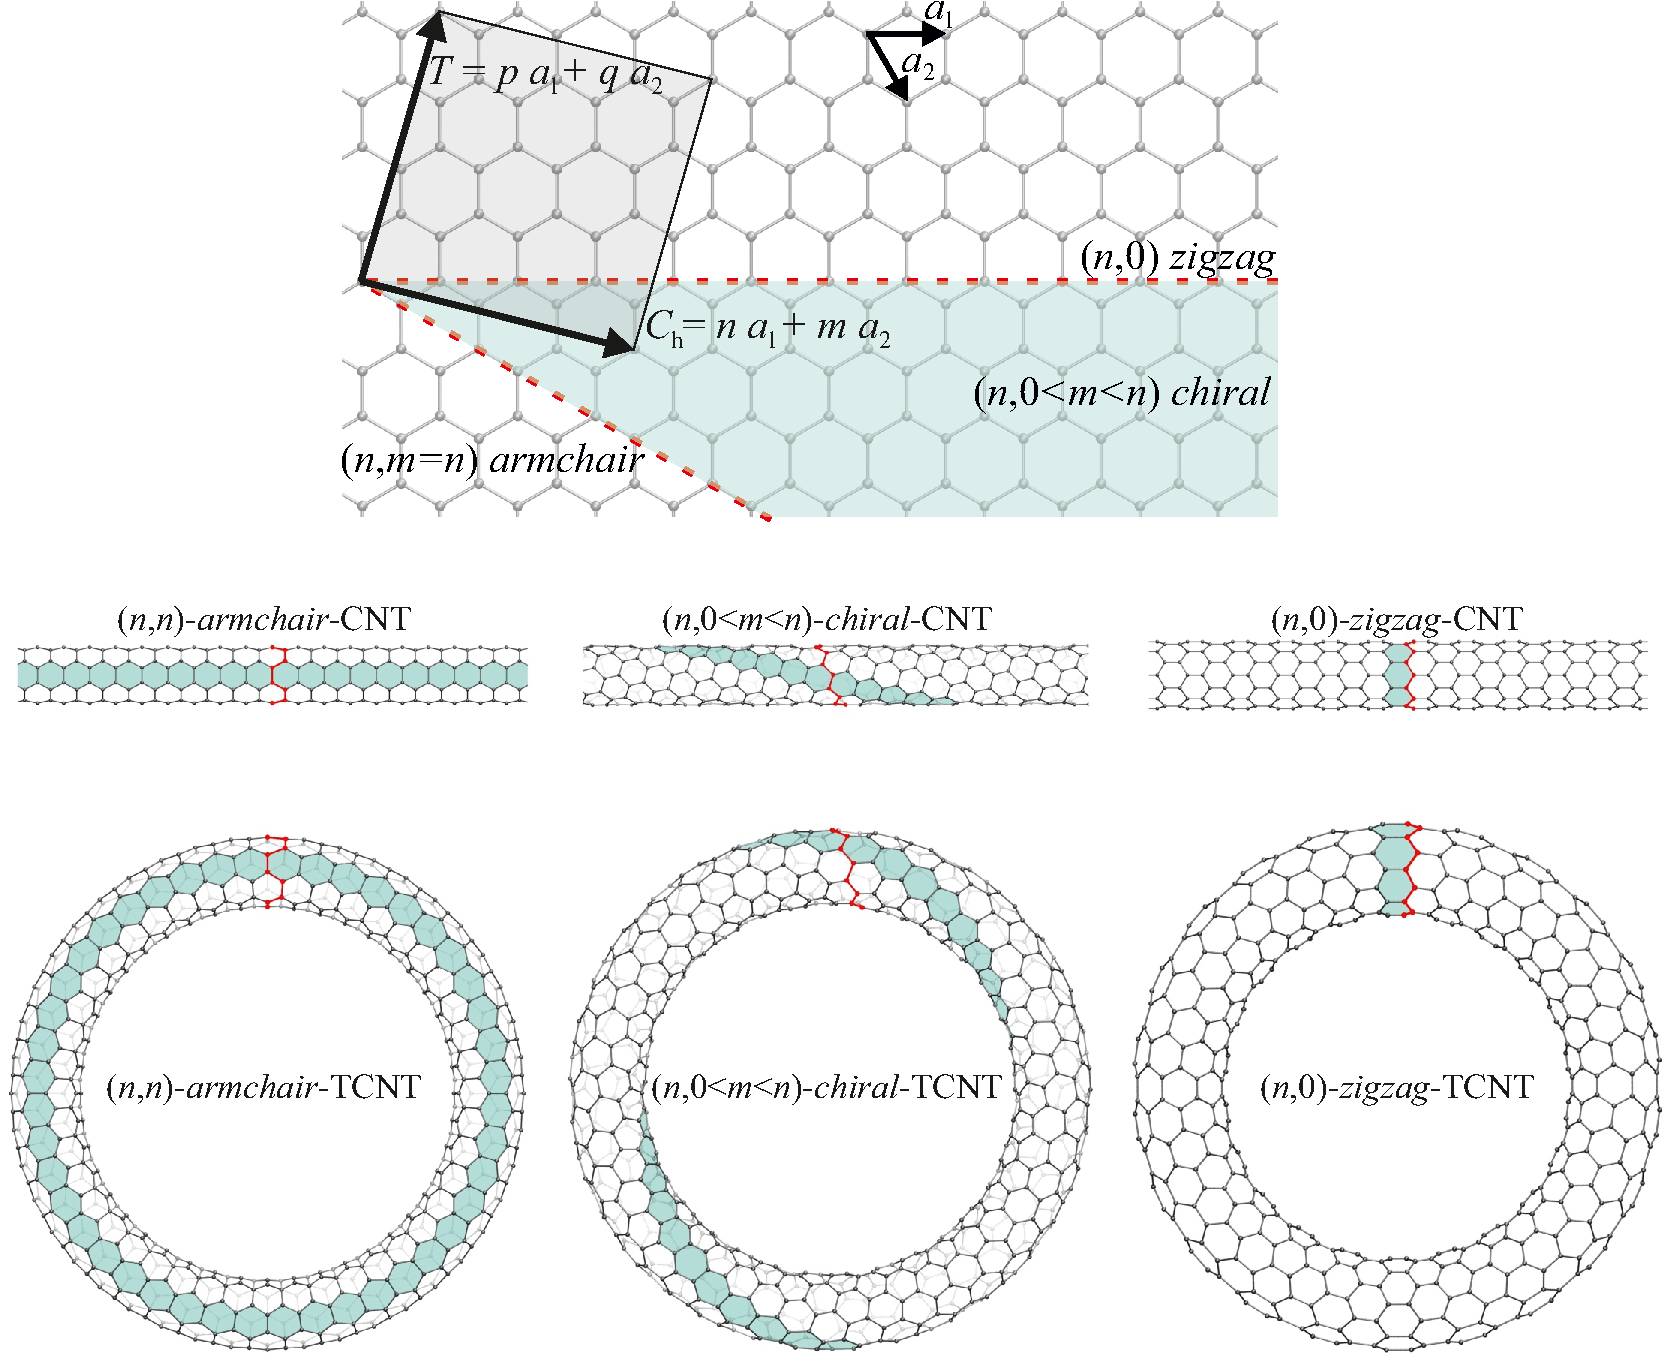
\includegraphics[width=1.0\textwidth]{vector}
	\captionsetup{figurewithin = chapter}
	\captionsetup{font=small, labelfont=bf}\caption[Konstruktionsschema von (toroidalen) Kohlenstoff Nanoröhren]{Allgemeines Konstruktionsschema für Kohlenstoff Nanoröhren (oben). $a_1$ und $a_2$ sind die Basisvektoren der Elementarzelle von Graphen. Der Chiralitätsvektor $\vec{\text{C}}_\text{h}$ liegt in dem türkis eingefärbten Bereich und die gestrichelten roten Linien geben die achiralen Grenzfälle (\textit{armchair} und \textit{zigzag}) an. Der Vektor $\vec{\text{T}}$ beschreibt die Länge von finiten Röhren und $n,m,p,q$ sind ganze Zahlen. Die grau eingefärbte Fläche definiert damit eine (n=3,m=1)(p=3,q=-4) \ac{cnt}. Struktur von \acp{cnt} (Mitte) und zu Ringen gebogene \acp{tcnt} (unten) mit unterschiedlichen Chiralitätsvektoren.}
\label{abb:chiralvector}
\end{figure}

Bereits kurz nach Entdeckung der Kohlenstoff Nanoröhren rückten auch gebogene Strukturen immer mehr in den Fokus der Forschung. Experimentell beobachtete \acp{cnt} beinhalten  beispielsweise auch fünf- und siebengliedrigen Kohlenstoffringen.\supercite{ichihashi1992pentagons} Diese Defekte führen zu positiven bzw. negativen Krümmungen wodurch verbogene und verdrillte Strukturen entstehen. Eine besonderer Strukturtyp sind die ringförmigen oder toroidalen \acp{cnt} (englisch \ac{tcnt}), erstmals beobachtet von Liu.\supercite{liu1997c} Seitdem wurden mehrere Methoden zur Erstellung solcher \acp{tcnt} vorgestellt, darunter \textit{Laser-growth} Methoden,\supercite{liu1997c} Ultraschallbehandlungen,\supercite{martel1999rings,martel1999ring} organische Reaktionen,\supercite{sano2001ring,geng2008synthesis} thermische Zersetzung von Kohlenwasserstoffgas\supercite{ahlskog1999ring} und \ac{cvd}\supercite{song2006large,zhou2006ring}. Diese \acp{tcnt} haben einen Torusdurchmesser von einigen hundert nm und einen Röhrendurchmesser von etwa \unit[5-20]{nm} und können aus einwandigen \ac{cnt} (englisch \ac{swnt}),\supercite{martel1999rings,martel1999ring,sano2001ring,geng2008synthesis,komatsu2006ultrasonic,guo2007spontaneously} zweiwandigen,\supercite{colomer2003rings} dreiwandigen\supercite{yu2006rings} oder mehrwandigen\supercite{ahlskog1999ring} \ac{cnt} bestehen. Weitere Strukturtypen sind auch in einem kürzlich erschienen Review\supercite{liu2014curved} zusammengefasst.
Aufgrund ihrer Ringförmigen Geometrie ist es denkbar, dass \acp{tcnt} andere mechanische, magnetische oder elektronische Eigenschaften als die geraden \acp{cnt} aufweisen und damit potentiell anderweitig Anwendung finden können.\supercite{liu2014curved}.
Bereits vor der experimentellen Generierung der\ac{tcnt} wurden auch auf theoretische Ebene unterschiedliche Strukturtypen vorgeschlagen. Diese lassen sich zum einen in perfekt toroidale Strukturen, welche nur aus sechsgliedrigen Ringen und damit aus gebogenen perfekten \acp{cnt} bestehen, und zum anderen in Strukturen welche fünf- und siebengliedrige Kohlenstoffringe enthalten aufteilen. Dunlab\supercite{dunlap1992connecting} schlug 1992 die Verknüpfung von (n,n) und (2n,0) \ac{cnt} vor, was zur Einführung von fünf- und siebengliedrigen Kohlenstoffringen und damit zur Bildung eines Torus führt. Zur Überprüfung einer möglichen Existenz wurden zahlreiche theoretische Studien über die thermodynamische Stabilität der \ac{tcnt} durchgeführt. Diese Studien zeigen, dass \ac{tcnt} stabiler als das C$_{60}$ Fulleren\supercite{dunlap1992connecting,itoh1993toroidal,ihara1993toroidal,itoh1993toroidal2} sein können und \ac{md} Simmulationen\supercite{itoh1993toroidal,hod2003carbon,tacsci2005stability,chen2011thermal} sagen eine Beständigkeit der Struktur bis ca \unit[2000]{K} voraus. Im Bezug auf die Rotationssymmetrie der \ac{tcnt} haben sich $D_{\text{6h}}$-symmetrische Strukturen als besonders Vorteilhaft herausgestellt\supercite{liu2011structure,ihara1995helically}, da die darin auftretenden Winkel den natürlichen Winkeln im Graphen am nächsten kommen und die geringste Verzerrung entsteht. 

Theoretisches limit für den Durchmesser \unit[200]{nm}\supercite{meunier1998atomic}

%Experimentell
Ring Bildung von experimentell erzeugten CNT \unit[0.5]{$\mu$m} Durchmesser, \unit[20]{nm} Dicke\supercite{ahlskog1999ring} durch thermische Zersetzung von Kohlenwasserstoff Gas. Hauptsächlich mehrwandig vermutlich keine perfekten Toren

%Eigenschaften
Je nach Ausrichtung des Chiralitätsvektors sind die \ac{cnt} entweder metallisch oder halbleitend. Für die \supercite{saito1998physical} \ac{tcnt} welche durch biegen von (n,m) \ac{cnt} entstehen, kann die elektronische Struktur im Bezug aufdie Vektoren $\vec{C}_h$ (n,m) und $\vec{T}$ (p,q) bestimmt werden.\supercite{ceulemans2000electronic} Für n-m=3i und p-q=3i (wobei i eine ganze Zahl sein muss) sind die \ac{tcnt} metallisch, für n-m=3i und p-q$\neq$3i sind sie Halbleiter und für n-m$\neq$3i und p-q=3i sind sie Isolatoren; n-m$\neq$3i und p-q$\neq$3i \ac{tcnt} existieren nicht.\supercite{zhang2005electronic} Für \ac{tcnt} mit fünf- und siebengliedrigen Kohlenstoffringen werden aufgrund der Ladungslokalisation an diesen Defektstellen üblicherweise HOMO-LUMO Lücken erhalten.\supercite{meunier1998atomic,oh2000structures,yazgan2004electronic,wu2011density} Aufgrund ihrer einzigartigen ringförmigen Geometrie sind auch die magnetischen Eigenschaften von \ac{tcnt} von großem Interesse. Haddon fand in dem von Dunlap vorgeschlagenen C$_{576}$ eine besonders große und anisotropische diamagnetische Ringstrom Suszeptibilität.\supercite{haddon1997electronic} Extrem große paramagnetische Momente wurden später von Liu \textit{et al.}\supercite{liu2002colossal} in metallischen \ac{tcnt} vorhergesagt. Grundsätzlich hängen die magnetischen Eigenschaften von \ac{tcnt} von Strukturellen Parametern wie dem Ringdurchmesser, der Krümmung, der Chiralität und auch von der Anordnung der fünf- und siebengliedrigen Kohlenstoffringe im Torus ab.\supercite{tsai2004magnetization,liu2007magnetic,liu2008magnetic}

Zwei unterschiedliche Flussrichtungen, latitudinal um das zentrale Loch und longitudinal, die aussen- und innenseite des Torus verbindend. Letztes hat die Symmetrie eines Dipolmoments und führt zu einem Anapol\supercite{ceulemans1998molecular} (Theorie) 

%Anwendungen
Auf theoretischer Ebene wurden ebenfalls unterschiedliche Einsatzgebiete für \ac{tcnt} untersucht. Darunter findet sich beispielsweise die Verwendung als Wasserstoffspeicher\supercite{castillo2010hydrogen,cruz2010hydrogen}. Aufgrund ihrer reversiblen elastischen Eigenschaften sind die \ac{tcnt} auch potentielle Kandidaten für ultrasensitive Kraftsensoren und flexible, dehnbare Nanogeräte. Ihre magnetischen Eigenschaften machen einen Einsatz als elektromagnetische Oszillatoren denkbar.\supercite{liu2014curved}

Mit Hilfe berechneter Ringströme lassen sich Aussagen über die Aromatizität eines Systems bzw. über die Delokalisierung der Elektronen darin treffen. Wie weiter oben erwähnt wurde,  sind die elektronischen und magnetischen Eigenschaften von \ac{tcnt} von besonderem Interesse, auch im Hinblick auf zukünftige Anwendungsmöglichkeiten dieser Systeme. Die in dieser Arbeit implementierten Methoden zur Reduzierung der Rechenzeit machen eine effiziente Berechnung der magnetischen Response möglich. Damit besteht nun die Möglichkeit Ringströme für aus mehreren hundert Kohlenstoffatomen bestehende \ac{tcnt} auf \ac{dft}-Niveau zu berechnen.

 Im Folgenden wird die Elektronendelokalisierung in einer Reihe unterschiedlicher \ac{tcnt} untersucht. Dabei werden sowohl nur aus sechsgliedrigen Kohlenstoffringen bestehende \ac{tcnt} berücksichtigt die aus gebogenen \ac{cnt} gebildet werden als auch \ac{tcnt} mit fünf- und siebengliedrigen Kohlenstoffringen. Letztere stellen bei den betrachteten Systemen die energetisch günstigeren Strukturen dar, da aufgrund der fünf- und siebengliedrigen Kohlenstoffringe Spannung aus dem System genommen wird. Die Untersuchungen beschränken sich dabei auf achirale \ac{tcnt} (\textit{armchair} und \textit{zigzag}) Strukturtypen. 


\chapter{Zusammenfassung}\label{zusammenfassung}
Im Rahmen der vorliegenden Arbeit konnte die Funktionalität des Moduls \texttt{mpshift} deutlich erweitert und die Effizienz bei den Berechnungen maßgeblich gesteigert werden. Durch die Implementierung des \acf{cosmo} besteht nun die Möglichkeit, Umgebungseffekte bei der Berechnung von Abschirmungskonstanten einzubeziehen. Zusätzlich ermöglicht dieses Modell die Kompensation von Gegenionen, was insbesondere für hoch geladene anionische Verbindungen wichtig ist. Darüber hinaus wurde das \acf{dcosmors} implementiert und in einer ausführlichen Studie mit dem \ac{cosmo} verglichen. Es konnte jedoch kein klarer Favorit innerhalb der beiden Methoden ausgemacht werden.

\bigskip
Die Implementierung von \acfp{ecp} ermöglicht nun die Berechnung von Abschirmungskonstanten in Molekülen, welche schwere Elemente beinhalten, ohne große All-Elektronen-Basissätze verwenden zu müssen. Auf diese Weise wird zusätzlich die Auswirkung relativistischer Effekte auf die Abschirmungskonstanten der Nachbaratome schwerer Elemente berücksichtigt. Die Eichinvarianz der Implementierung wurde anhand der Abschirmungskonstanten in Co(ppy)$_3$ (ppy=2-Phenylpyridin) demonstriert. 

\bigskip
Das Modul \texttt{mpshift} kann nun ebenfalls die Response der Wellenfunktion auf ein äußeres Magnetfeld, welche zur Berechnung von \ac{vcd}-Spektren benötigt wird, bereitstellen. Die eigentliche Berechnung der \ac{vcd}-Spektren wurde in das im Modul \texttt{aoforce} implementiert. Der Vergleich zwischen dem experimentellen \ac{vcd}-Spektrum und den simulierten \ac{vcd}-Spektren von \acl{cpa} zeigt, dass die effiziente Basissatz/Funktional-Kombination def2-SV(P)/BP86 qualitativ gleichwertige Spektren liefert wie die deutlich aufwändigere Kombination def2-TZVP/B3LYP. Die effiziente Implementierung aus der vorliegenden Arbeit erlaubt beispielsweise die Berechnung der \ac{vcd}-Spektren von großen $I$-symmetrischen Fullerenen. Darunter ist das C$_{620}^{2+}$ mit 8680 Basisfunktionen das bislang größte System, für welches ein \ac{vcd}-Spektrum berechnet wurde.

Des Weiteren wurde das Modul \texttt{mpshift} in Zusammenarbeit mit Fabian Mack im Rahmen seiner Masterarbeit um die Möglichkeit erweitert, Abschirmungskonstanten mithilfe von \ac{mgga}-Funktionalen zu berechnen. 
\vfill
\newpage
Durch die Implementierung der \ac{ri}- und \ac{marij}-Näherungen konnte eine hoch effiziente Berechnung des Coulombbeitrages erreicht werden. Dies führt beispielsweise bei der Berechnung der Abschirmungskonstanten eines \ac{rns}-Segments mit 1018 Atomen und 10220 Basisfunktionen zu einer Rechenzeitbeschleunigung des Coulombbeitrages um einen Faktor größer als 100, ohne einen nennenswerten Verlust an Genauigkeit. Die Gesamtrechenzeit reduziert sich damit von \unit[43.2]{h} auf \unit[7.6]{h}. Neben weiteren Optimierungen des Programmcodes konnte die Anzahl der benötigten Iterationen beim Lösen der \ac{cphf}-Gleichungen leicht verringert werden. Für Hartree-Fock- bzw. Hybrid-\ac{dft}-Rechnungen wurde zudem eine effizientere Integralabschätzung auf die Berechnung der nach den Komponenten des Magnetfeldes abgeleiteten Austauschmatrixelemente übertragen. Die Berechnung der Abschirmungskonstanten für eine Kette von 48 $\alpha$-\textsc{d}-Glucose-Einheiten mit dem B3LYP-Funktional benötigt mit der vorliegenden Implementierung \unit[5.75]{h} auf einer einzelnen CPU. Dies ist ein Bruchteil der für andere Implementierungen (Referenzen \cite{beer2011nuclei} und \cite{kumar2016nuclei}) publizierten Zeiten für die identischen Rechnungen. Mit der vorliegenden Implementierung lassen sich die Abschirmungskonstanten von Systemen mit mehreren tausend Atomen innerhalb weniger Tage auf (Hybrid-)\ac{dft}-Niveau unter Verwendung einer \textit{double}-$\zeta$-Basis berechnen. Der Aufwand für die Berechnung der chemischen Verschiebungen liegt nun oft unter dem für die vorangehende Berechnung der Wellenfunktion. Zusätzlich wurden alle zeitbestimmenden Routinen im Modul \texttt{mpshift} parallelisiert, um die Rechnungen auf mehreren Prozessoren zu ermöglichen.

\bigskip
Die im Rahmen der vorliegenden Arbeit erreichte Effizienzsteigerung ermöglicht zudem die Berechnung von Ringströmen zur Untersuchung magnetischer Eigenschaften in großen toroidalen Kohlenstoff-Nanoröhren (englisch \acfp{tcnt}) mit bis zu ca. 1000 Kohlenstoffatomen. Das sind nach meinem Kenntnisstand die bislang größten Systeme, für welche Ringströme berechnet wurden. 

Es zeigte sich, dass ein möglichst kleines HOMO-LUMO-Gap eine notwendige -- aber nicht hinreichende -- Bedingung für das Vorhandensein eines Gesamtringstromes  ist. Dadurch werden insbesondere metallische \acp{tcnt} zu vielversprechenden Kandidaten. In der Tat wurden für letztere große (vorwiegend diatropische) Ringströme berechnet, aber auch für die von Dunlap vorgeschlagenen $D_{\text{6h}}$-symmetrischen \acp{tcnt}. Grundsätzlich hängen Ringströme stark von den strukturellen und elektronischen Eigenschaften der Systeme ab, beispielsweise von der Orientierung und Lage der fünf- und siebengliedrigen Ringe. Bei den Untersuchungen konnte außerdem gezeigt werden, dass der Ringstrom mit zunehmendem Torusdurchmesser an Stärke gewinnt. 
\vfill
\newpage
Ringströme wurden ebenfalls für das Anion [Hg$_8$Te$_8$(Te$_2$)$_4$]$^{8-}$ berechnet, welches in der Arbeitsgruppe Dehnen (Universität Marburg) synthetisiert wurde und dessen Struktur an das Porphyrin erinnert. Es zeigte sich, dass bei diesem Molekül, anders als bei Porphyrin, kein globaler Ringstrom auftritt, sondern nur schwache lokale Ringströme in den fünfgliedrigen Ringen. Dies bedeutet, dass die Elektronen nicht über das gesamte Molekül delokalisiert sind und damit keine globale Aromatizität vorliegt. 

Zwei weitere Anwendungen des Programms auf anorganische Systeme beschäftigten sich mit der Erklärung von $^{31}$P-chemischen Verschiebungen sowie der Zuordnung von $^{119}$Sn-chemischen Verschiebungen in den endohedralen Clusteranionen [Co@Sn$_6$Sb$_6$]$^{3-}$ und [Co$_2$@Sn$_5$Sb$_7$]$^{3-}$.

\bigskip
Diese Beispiele zeigen, dass die in der vorliegenden Arbeit implementierten Methoden erfolgreich auf chemische Fragestellungen angewendet werden können. Näherungsverfahren sowie Programmoptimierungen und -parallelisierung erlauben die Berechnung von \ac{nmr}-Abschirmungstensoren für sehr große System mit vergleichsweise geringem Zeitaufwand. Die Erweiterungen der Funktionalität ermöglichen die Berechnung chemischer Verschiebungen von Atomen in Molekülen, welche schwere Elemente beinhalten oder hoch geladen sind. Umgebungseffekte können auf unterschiedliche Weise berücksichtigt werden und simulierte \ac{vcd}-Spektren ermöglichen die Bestimmung absoluter Konfigurationen in chiralen Molekülen.
\vfill
\newpage
\thispagestyle{empty}
\cleardoublepage


% Schlussteil - Römische Seitennummerierung
\backmatter
%\pagenumbering{Roman}
%\setcounter{page}{9}

\begingroup
	\renewcommand*{\addvspace}[1]{}
	\phantomsection
	\listoffigures
\endgroup

\begingroup
	\renewcommand*{\addvspace}[1]{}
	\phantomsection
	\listoftables
\endgroup
\newpage
\phantomsection \addcontentsline{toc}{chapter}{Abkürzungsverzeichnis}
\renewcommand\refname{Abkürzungsverzeichnis} \chapter*{Abkürzungsverzeichnis}
\begin{acronym}[SEPSEP] % längste Abkürzung steht in eckigen Klammern
    \setlength{\itemsep}{0.2cm} % geringerer Zeilenabstand
    
    \acro{aat}[AAT]{\textit{atomic axial tensor}}
    
    \acro{apt}[APT]{\textit{atomic polar tensor}}
    
    \acro{ao}[AO]{Atomorbital}
	\acro{caac}[CAAC]{cyclisches Alkylaminocarben}   
		\acrodefplural{caac}[CAACs]{cyclischen Alkylaminocarbenen}
	\acro{carac}[CArAC]{cyclisches Arylaminocarben}
		\acrodefplural{carac}[CArACs]{cyclische Arylaminocarbene}
		
    \acro{cc}[CC]{Coupled Cluster}		
		
 	\acro{cosmo}[COSMO]{\textit{Conductor-like Screening Model}}
 	
	\acro{cphf}[CPHF]{\textit{coupled perturbed Hartree-Fock}}
 	
    \acro{dft}[DFT]{Dichtefunktionaltheorie}
    
    \acro{dipp}[dipp]{2,6-Diisopropylphenyl}
    
    \acro{ecp}[ECP]{\textit{Effective-Core-Potential}}
    
    \acro{esp}[ESP]{elektrostatisches Potential}
	    \acrodefplural{esp}[ESP]{elektrostatischen Potentials}
	
	\acro{giao}[GIAO]{\textit{Gauge Including Atomic Orbital}}   
	
	\acro{gimic}[GIMIC]{\textit{Gauge Including Magnetically Induced Currents}} 

	\acro{gga}[GGA]{\textit{Generalized-Gradient-Approximation}}   
		\acrodefplural{gga}[GGA]{\textit{Generalized-Gradient-Approximation}}
		
	\acro{lcao}[LCAO]{\textit{Linear Combination of Atomic Orbitals}}
	\acro{lda}[LDA]{\textit{Local-Density-Approximation}}
     
    \acro{marij}[MARI-J]{\textit{Multipole Accelerated Resolution of the Identity for $J$}} 	
 	
	\acro{mgga}[MGGA]{\textit{Meta}-GGA}   
		\acrodefplural{mgga}[MGGA]{\textit{Meta}-GGA}	
	\acro{mo}[MO]{Molekülorbital}   
		\acrodefplural{mo}[MOs]{Molekülorbitale}
		
	\acro{mp2}[MP2]{M\o ller-Plesset Störungstheorie zweiter Ordnung}
		
    \acro{nao}[NAO]{\textit{Natural-Atomic-Orbital}}

    \acro{nbo}[NBO]{\textit{Natural-Bond-Orbital}}
    
    \acro{nmr}[NMR]{\textit{Nuclear Magnetic Resonace}}
        
    \acro{npa}[NPA]{\textit{Natural-Population-Analysis}}
    
    \acro{oswo}[OWSO]{\textit{Occupancy-Weighted-Symmetric-Orthogonalization}}
    
    \acro{ri}[RI]{\textit{Resolution of the Identity}}
    
	\acro{scf}[SCF]{\textit{Self Consistent Field}}   

	\acro{tep}[TEP]{Tolmans elektronischer Parameter}   
		\acrodefplural{tep}[TEPs]{Tolmans elektronische Parameter}
		
	\acro{vcd}[VCD]{\textit{Vibrational Circular Dichroism}}

    

        
    \acro{vmd}[VMD]{Visual Molecular Dynamics}
\end{acronym}

\printbibliography[title=Literaturverzeichnis]

\chapter*{Veröffentlichungen}
\markboth{Veröffentlichungen}{} %chapterheader trotz * anzeigen lassen
\begin{enumerate}
%\item \textit{•}\\ \textit{•} \textbf{•}

\item \textit{Controlling the Dimensionality in Au(I)-Tl(I) Metallopolymers}\\
T. Seifert, N. Knoefel, T. Feuerstein, K. Reiter, S. Lebedkin, A. Boukis, F. Weigend, M. Kappes, P. Roesky, \textit{•} \textbf{•}, in Vorbereitung (2018).
[Co@Sn$_6$Sb$_6$]$^{3-}$:
\item \textit{[Co@Sn$_6$Sb$_6$]$^{3-}$: Structure and $^{119}$Sn NMR Spectrum of an Off-Center Endohedral 12-Vertex Cluster}\\
R. J. Wilson, F. Hastreiter, K. Reiter, P. Büschelberger, R. Wolf, R. Gschwind, F. Weigend, S. Dehnen, \textit{•} \textbf{•}, eingereicht (2018).

\item \textit{[Hg$_4$Te$_8$(Te$_2$)$_4$]$^{8-}$: A Heavy Metal Porphyrinoid Embedded in a Lamellar Structure}\\
C. Donsbach, K. Reiter, D. Sundholm, F. Weigend, S. Dehnen, \textit{Angew. Chem. Int. Ed.} \textbf{57}, 8770–8774, (2018).

\item \textit{Multicomponent Reactions Provide Key Molecules for Secret Communication}\\ 
A. Boukis, K. Reiter, M. Frölich, D. Hofheinz, M. Meier, \textit{Nat. Commun.} \textbf{9}, 1439 (2018).

\item \textit{(Ge$_2$P$_2$)$^{2-}$: A Binary Analogue of P$_4$ as a Precursor to the Ternary Cluster Anion [Cd$_3$(Ge$_3$P)$_3$]$^{3-}$}\\
S. Mitzinger, J. Bandemehr, K. Reiter, J. McIndoe, X. Xie, F. Weigend, J. Corrigan, S. Dehnen, \textit{Chem. Commun.} \textbf{54}, 1421-1424 (2018).

\item \textit{Calculation of Magnetic Shielding Constants with meta-GGA Functionals Employing the Multipole-Accelerated Resolution of the Identity: Implementation and Assessment of Accuracy and Efficiency}\\ 
K. Reiter, F. Mack, F. Weigend, \textit{J. Chem. Theory Comput.} \textbf{14}, 191-197 (2018).

\item \textit{An NHC-Phosphinidenyl as a Synthon for New Group 13/15 Compounds}\\
O. Lemp, M. Balmer, K. Reiter, F. Weigend, C. von Hänisch, \textit{Chem. Commun.} \textbf{53}, 7620-7623 (2017).

\item \textit{Vibrational Circular Dichroism Spectra for Large Molecules and Molecules with Heavy Elements}\\
K. Reiter, M. Kühn, F. Weigend, \textit{J. Chem. Phys.} \textbf{146}, 054102 (2017).

\item \textit{A Dinuclear Gold(I) Bis(Carbene) Complex Based on a Ditopic Cyclic (Aryl)\\(Amino)Carbene Framework}\\
E. Deck, K. Reiter, W. Klopper, F. Breher, \textit{Z. Anorg. Allg. Chem.} \textbf{642}, 1320-1328 (2016).

\item \textit{A Boron-Fluorinated Tris(pyrazolyl)borate Ligand ($^FTp^*$) and Its Mono- and Dinuclear Copper Complexes [Cu($^FTp^*$)$_2$] and [Cu$_2$($^FTp^*$)$_2$]: Synthesis, Structures, and DFT Calculations}\\
T. Augenstein, F. Dorner, K. Reiter, H. Wagner, D. Garnier, W. Klopper, F. Breher, \textit{Chem. Eur. J.} \textbf{22}, 7935-7943 (2016).

\item \textit{[(Pb$_6$I$_8$)\{Mn(CO)$_5$\}$_6$]$^{2-}$: An Octahedral (M$_6$X$_8$)-like Cluster with Inverted Bonding}\\
S. Wolf, K. Reiter, F. Weigend, W. Klopper, C. Feldmann, \textit{Inorg. Chem.} \textbf{54}, 3989-3994 (2015).
\end{enumerate}

\chapter*{Lebenslauf}
\markboth{Lebenslaug}{} %chapterheader trotz * anzeigen lassen
\renewcommand{\arraystretch}{1.7}
\begin{singlespace}
\begin{tabular}{lp{7.6cm}}
Name: & Kevin Reiter \\ 

Geburtsdatum: & 29. November 1989 \\ 

Geburtsort: & Neuenbürg \\ 

\quad & \quad \\

1996 - 2000 & Wilhelm-Ganzhorn-Grundschule Straubenhardt \\ 

2000 - 2009 & Gymnasium Neuenbürg \\ 

Juni 2009 & allgemeine Hochschulreife \\ 

2010 - 2013 & Bachelor Studium Chemie am Karlsruher Institut für Technologie  \\ 
Juni 2013 - August 2013  & Bachelorarbeit am Institut für Physikalische Chemie, Abteilung für Theoretische Chemie am Karlsruher Institut für Technologie unter Anleitung von Prof. Dr. Willem Klopper \\

Oktober 2013 & Abschlus als Bachelor of Science \\ 
 
2013 - 2015 & Master Studium Chemie am Karlsruher Institut für Technologie \\ 

März 2015 - September 2015  & Masterarbeit am Institut für Physikalische Chemie, Abteilung für Theoretische Chemie am Karlsruher Institut für Technologie unter Anleitung von Prof. Dr. Willem Klopper \\

September 2015 & Abschlus als Master of Science \\ 

2015 & Beginn der Promotion am Institut für Physikalische Chemie, Abteilung für Theoretische Chemie am Karlsruher Institut für Technologie unter Anleitung von PD Dr. Florian Weigend \\ 

November 2017 - Dezember 2017 & 6-wöchiger Forschungsaufenthalt an der Universität Helsinki bei Prof. Dr. Dage Sundholm \\ 
\end{tabular}  
\end{singlespace}
\enlargethispage{13.5pt}
\vfill
\newpage
\thispagestyle{empty}
\quad
\chapter*{Danksagung}
\markboth{Danksagung}{} %chapterheader trotz * anzeigen lassen
%\thispagestyle{empty}
Zu Beginn möchte ich mich bei meinen Mathematik-, Physik- und Chemielehrern Michael Frey, Matthias Sickmüller und Michael Burkard bedanken, die zur rechten Zeit mein Interesse an den Naturwissenschaften gefördert und gefordert haben. Ich danke ihnen für ihren lehrreichen und vorbildlichen Unterricht, auch wenn das einige meiner ehemaligen Mitschüler sicher anders sehen würden.

\bigskip
Mein größter Dank gilt PD Dr. Florian Weigend für eine Betreuung, wie sie nicht hätte besser sein können. Insbesondere für seine unermüdliche Unterstützung bei noch so kleinen Fragen und Problemen, all die anregenden Gespräche und auch für die Freiheiten, die er mir gelassen hat. Die Momente abseits der Wissenschaft und die Vermittlung der wirklich wichtigen Kompetenzen -- am Kickertisch -- werden mir immer in bester Erinnerung bleiben. Eine wahrhaft vorbildliche Zusammenarbeit zwischen einem Schwaben und einem Badener.

\bigskip
Prof. Dr. Burkhard Luy danke ich vielmals für die Übernahme des Koreferats.

\bigskip
Bei Prof. Dr. Willem Klopper möchte ich mich für die Finanzierung zu Beginn meiner Promotion bedanken. Weiterhin danke ich ihm für die Nutzung der am Lehrstuhl für Theoretische Chemie zur Verfügung stehenden Ressourcen. Nicht zuletzt bin ich dankbar für die Zeit und die Betreuung während meiner Bachelor-, Vertiefungs- und Masterarbeit, was mein Interesse an der Theoretischen Chemie vertieft und letztlich zu dieser Arbeit geführt hat.

\bigskip
Besonderer Dank gilt meinem langjährigen Bürokollegen Christof Holzer mit dem ich nun seit einiger Zeit das \glqq vormals Badisch Birro\grqq{} besetze. Es war und ist eine tolle Zeit zusammen mit ihm, sowohl im Büro als auch auf diversen Konferenzen oder Wanderungen, egal ob in Mariapfarr, Bochum, München oder Helsinki.

\bigskip
Dr. Markus Armbruster danke ich für die gemeinsame Zeit im damals noch \glqq Badische Birro\grqq{} und seine Hilfsbereitschaft meine Fragen zu beantworten. 

Dr. Michael Kühn und Fabian Mack danke ich für die Zusammenarbeit am VCD- und meta-GGA-Projekt.  

\bigskip
Prof. Dr. Dage Sundholm danke ich für seine Gastfreundschaft während meiner beiden Aufenthalte in Helsinki sowie für die Betreuung während meines Forschungsaufenthalts. In diesem Zusammenhang sollen auch Maria Dimitrova und Dr. Lukas Wirz nicht unerwähnt bleiben.
%\newpage
%\thispagestyle{empty}

Dr. Michael Harding, Frank Imhoff und Sebastian Kleinhans gilt mein Dank für alle technischen Angelegenheiten sowie für die Lösung von Problemen bei Soft- und Hardwarefragen. 

Weiter danke ich allen zeitweiligen oder noch aktiven Mitgliedern in der Abteilung für Theoretische Chemie, die ich während meiner Zeit dort -- seit meiner Bachelorarbeit -- kennenlernen durfte, für die tolle Zeit und auch für die nicht immer fachlichen Gespräche. Dazu gehören insbesondere Dr. Angela Bihlmeier, Dr. Katharina Krause, Dr. Jiří Chemla, Dr. Johannes Heuser, Dr. Nils  Middendorf, Nils Schieschke, Dr. Patrik Pollak, Dr. Peter Limacher und Yannick Franzke.

Unserer Sekretärin Manuela Kühn danke ich für ihre Hilfe bei allen organisatorischen und bürokratischen Angelegenheiten, die sie immer gerne übernommen hat, obwohl ich eigentlich am INT im Norden angestellt bin.

\bigskip
Für die kritische und äußerst aufmerksame Durchsicht der Arbeit bedanke ich mich bei Fabian Mack, Dr. Johannes Heuser und Yannick Franzke.

\bigskip
Außerdem gilt mein Dank dem SFB 1176 \glqq Strukturierung weicher Materie\grqq{} der Deutschen Forschungsgemeinschaft (DFG) für die finanzielle Unterstützung.

\bigskip
Meinen Eltern und meiner Familie danke ich für das grenzenlose Vertrauen und die Unterstützung meiner Vorhaben seit jeher. 

\bigskip
Meiner Freundin Martina Hadamjetz danke ich für ihre bedingungslose Liebe und die wundervolle gemeinsame Zeit. 
%Schliesslich danke ich s`Madame fuer ihre Liebe :)

\newpage
\thispagestyle{empty}
\quad

%Abkürzungen ausgeben
\deftranslation[to=German]{Acronyms}{Abkürzungsverzeichnis}
\printglossary[type=\acronymtype,style=long]
% ---------------------------------------------------------------
% Anhang
\appendix
%\includepdf[pages=-,fitpaper=true,addtotoc={1,section,0,Diagramm: Vergabe,fig:Vergabedia}]{Pfad-zu-einem-pdf-dokument.pdf}
\end{document}